\documentclass[12pt]{scrbook}
\usepackage{amsmath}
\usepackage{bm}
\usepackage{colortbl}
\usepackage{graphicx}
\usepackage{caption}
\usepackage{fullpage}
\usepackage{afterpage}
\usepackage{float}
\usepackage{multirow}
\usepackage[nodisplayskipstretch]{setspace}
\usepackage{booktabs}
\usepackage{textcomp}
\usepackage{gensymb}
\usepackage[utf8]{inputenc} 
%\usepackage{parskip}
\usepackage{xr}
\usepackage{pdflscape}
\usepackage[labelfont=bf,tableposition=top]{caption}
\usepackage[inline]{enumitem}
\usepackage{wrapfig}
\usepackage{longtable}
\usepackage{subfig}
\usepackage[hidelinks]{hyperref}
\usepackage{geometry}
\usepackage{fancyhdr}
\usepackage[acronym,nomain,toc,makeindex ]{glossaries}
\usepackage{graphicx}
\usepackage[section]{placeins}
\usepackage{eufrak}
\usepackage[table]{xcolor} 
\usepackage{cmap}
\usepackage{cleveref} %This need to be the last package for it to work properly 
\usepackage[hyperref=true,maxcitenames=3,maxbibnames=3,url=false,doi=false,isbn=false,backref=true,natbib=true,backend=biber,sorting=nyvt,defernumbers=false, style=authoryear]{biblatex}
\setcounter{secnumdepth}{3}
%
%
%	TITLE PAGE DEFINITION
%
%
\renewcommand*\contentsname{Contents}
\setlength{\parindent}{4ex}
\newcommand{\rom}[1]{\uppercase\expandafter{\romannumeral #1\relax}}
\newcommand*{\glng}{\glsentrylong}
\newcommand*{\scz}{schizophrenia}
\newcommand*{\Scz}{Schizophrenia}
\newcommand*{\Glng}{\Glsentrylong}
\newcommand{\beginsupplement}{%
	\setcounter{table}{0}
	\renewcommand{\thetable}{S\arabic{table}}%
	\setcounter{figure}{0}
	\renewcommand{\thefigure}{S\arabic{figure}}%
}
\newcommand{\specialcell}[2][c]{\begin{tabular}[#1]{@{}c@{}}#2\end{tabular}}

%
%	GLOSSARY SECTION
%
\addbibresource[datatype=bibtex]{citation/citation.bib}
\makeglossary
\newacronym[longplural={Genome Wide Association Studies}]{GWAS}{GWAS}{Genome-Wide Association Study}
\newacronym{wgs}{WGS}{Whole Genome Sequencing}
\newacronym{SNP}{SNP}{Single Nucleotide Polymorphism}
\newacronym{LD}{LD}{Linkage Disequilibrium}
\newacronym{PGS}{PGS}{Polygenic Risk Score}
\newacronym{tSVD}{tSVD}{Truncated Singular Value Decomposition}
\newacronym{SVD}{SVD}{Singular Value Decomposition}
\newacronym{shrek}{SHREK}{SNP HeRitability Estimation Kit}
\newacronym{gcta}{GCTA}{Genome-wide Complex Trait Analysis}
\newacronym{ldsc}{LDSC}{LD SCore regression}
\newacronym{CEU}{CEU}{Northern Europeans from Utah}
\newacronym{se}{SE}{standard error}
\newacronym{maf}{MAF}{Minor Allele Frequency}
\newacronym{isc}{ISC}{International Schizophrenia Consortium}
\newacronym{mgs}{MGS}{Molecular Genetic of Schizophrenia}
\newacronym{sgene}{SGENE}{Schizophrenia Genetics Consortium}
\newacronym{pgc}{PGC}{Psychiatric Genomics Consortium}
\newacronym{rin}{RIN}{RNA integrity number}
\newacronym{gd}{GD}{Gestation Day}
\newacronym{rpkm}{RPKM}{Reads Per Kilobase per Million mapped reads}
\newacronym{wgcna}{WGCNA}{Weighted Gene Co-expression Network Analysis}
\newacronym{pc}{PC}{Principle Component}
\newacronym{GO}{GO}{Gene Ontology}
\newacronym{MAGMA}{MAGMA}{Multi-marker Analysis of GenoMic Annotation}
\newacronym{ngs}{NGS}{next generation sequencing}
\newacronym{dsm}{DSM}{Diagnostic and Statistical Manual of Mental Disorders}
\newacronym{mse}{MSE}{mean squared error}
\newacronym{who}{WHO}{World Health Organization}
\newacronym{yld}{YLD}{years lost due to disability}
\newacronym{ci}{CI}{confidence interval}
\newacronym{iq}{IQ}{Intelligence Quotient}
\newacronym{polyic}{PolyI:C}{polyriboinosinic-polyribocytidilic acid}
\newacronym{lps}{LPS}{lipopolysaccharide}
\newacronym{il6}{IL-6}{Interleukin-6}
\newacronym{mz}{MZ}{monozygotic}
\newacronym{dz}{DZ}{dizygotic}
\newacronym{mia}{MIA}{maternal immune activation}
\newacronym{ncp}{NCP}{non-centrality parameter}
\newacronym{cnv}{CNV}{copy number variation}
\newacronym{grm}{GRM}{Genetic Relationship Matrix}
\newacronym{gc}{GC}{Genomic Control}
\newacronym{mhc}{MHC}{major histocompatibility complex}
\newacronym{cns}{CNS}{central nervous system}
\newacronym{nmda}{NMDA}{N-methyl-D-aspartate}
\newacronym{eps}{EPS}{extrapyramidal motor symptoms}
\newacronym{pca}{PCA}{principle component analysis}
\newacronym{fdr}{FDR}{false discovery rate}
\newacronym{pcgc}{PCGC}{Phenotype correlation - genotype correlation regression}
\newacronym{ibd}{IBD}{identity by descent}
\newacronym{bp}{bp}{base pair}
\newacronym{mb}{mb}{megabase}
\newacronym{kb}{kb}{kilobase}
\newacronym{deg}{DEG}{differentially expressed gene}
\newacronym{qc}{QC}{quality control}
\newacronym{hku}{HKU}{the University of Hong Kong}
\newacronym{pcr}{PCR}{polymerase chain reaction}
\newacronym{ercc}{ERCC}{External RNA Controls Consortium}
\newacronym{go}{GO}{Gene Ontology}
\newacronym{rtpcr}{RT-PCR}{real time PCR}
\newacronym{ct}{CT}{cycle threshold}
\newacronym{geo}{GEO}{Gene Expression Omnibus}
\newacronym{mlm}{MLM}{mixed linear model}
\newacronym{reml}{REML}{restricted maximum likelihood}
\newacronym{pufa}{PUFA}{polyunsaturated fatty acid}
\newacronym{msigdb}{MSigDB}{Molecular Signatures Database}
\newacronym{fgf}{FGF}{fibroblast growth factor}
\newacronym{egf}{EGF}{epidermal growth factor}
\newacronym{pi3k}{PI3K}{phosphatidylinositol 3-kinase}
\newacronym{mapk}{MAPK}{mitogen-activated protein kinase}
\newacronym{gaba}{GABA}{$\gamma$-aminobutyric acid}
\newacronym{ecm}{ECM}{extracellular matrix}
\newacronym{mmp}{MMP}{matrix metalloproteinase}
\newacronym{qqplot}{QQ-plot}{quantile-quantile Plot}
\newacronym{cm}{cM}{centiMorgan}
\newacronym{pet}{PET}{positron emission tomography}
\newacronym{mrna}{mRNA}{messenger RNA}
\newacronym{psd}{PSD}{postsynaptic density}
\newacronym{kegg}{KEGG}{Kyoto Encyclopedia of Genes and Genomes}
\newacronym{arc}{ARC}{neuronal activity-regulated cytoskeleton-associated protein}
\newacronym{cb1}{CB1}{cannabinoid receptor type 1}
\newacronym{nih}{NIH}{National Institutes of Health}
%
%
%	FORMATING SECTION
%
%
\pagestyle{fancy}
\fancyhf{}
\fancyfoot[LE,RO]{\thepage}
\renewcommand{\footrulewidth}{1pt}
\fancyhead[LE]{\leftmark}
\fancyhead[RO]{\rightmark}

\geometry{
	top=1in,            % <-- you want to adjust this
	inner=1in,
	outer=3.5cm,
	bottom=3.5cm,
	headheight=3ex,       % <-- and this
	headsep=2ex,          % <-- and this
}

\raggedbottom %Remove it before printing as this is something to do with global settings. Can make each page look uneven but more dense. 
%\onehalfspacing
\doublespacing
\makeindex
\begin{document}\thispagestyle{empty}
\pagestyle{empty}
\begin{singlespace}
	\begin{titlepage}
		\begin{center}
			\vspace*{1cm}
			
			\Huge
			\textbf{The Genetics of Schizophrenia - The Contribution of Common Variants and Genes Implicated in a Maternal Immune Activation Model}
			
			\vspace{0.5cm}
			\LARGE
			
			\vspace{1.5cm}
			
			\textbf{\href{mailto:choishingwan@gmail.com}{Choi Shing Wan}}
			
			\vfill
			
			A thesis submitted in partial fulfillment of the requirements for \\
			the Degree of Doctor of Philosophy
			
			\vspace{0.8cm}
			
			
\includegraphics[width=0.4\textwidth]{figure/hkuLogo.jpg}
			
			\Large
			Department of Psychiatry\\
			University of Hong Kong\\
			Hong Kong\\
			\today
		\end{center}
	\end{titlepage}
\end{singlespace}

\frontmatter 
\cleardoublepage
\phantomsection
\addcontentsline{toc}{chapter}{Abstract}
\chapter*{\centerline{Abstract}}
\vspace{0.1cm}
Schizophrenia is a disabling disorder affecting approximately 1\% of the population worldwide.
Twins studies and family studies estimated that genetic factors contributes to 64\%-80\% of the liability of \scz.
With the development of \gls{GWAS}, a total of 108 common genetic loci associated with \scz\ has been identified through the meta-analysis conducted by the \Scz\ Working Group of \gls{pgc}. 
Using the summary statistic from the \gls{pgc} \scz\ \gls{GWAS}, \citet{Bulik-Sullivan2015} estimated that the common variant contributes to around 55.5\% of the liability of \scz\ using \gls{ldsc}.
However, studies suggest that rare mutations, structural variance, \gls{cnv} and also genetic-environment interaction are all contributing to the risk of \scz.
This suggest that the estimate from \citet{Bulik-Sullivan2015} might be too high.
An independent estimation of the \gls{SNP}-heritability of \scz\ might provide insight as to whether if estimates from \citet{Bulik-Sullivan2015} are inflated.

In this thesis, we developed \gls{shrek}, an alternative algorithm for the estimation of \gls{SNP}-heritability.
Our simulation results suggest that, \gls{shrek} provided a more robust estimate for oligogenic traits and for binary traits when no confounding variables was present when compared to \gls{ldsc}. 
Most importantly, using the summary statistics from the \scz\ \gls{GWAS}, the \gls{SNP}-heritability of \scz\ is estimated to be 0.185 (SD=0.00450) by \gls{shrek} and 0.198 (SD=0.0057) by \gls{ldsc}, suggesting that the estimates from \citet{Bulik-Sullivan2015} are inflated.
Thus, the common variants contributes to less than 20\% of the liability of \scz\ and it is likely for other genetic variants such as rare mutations and epigenetic factors to contribute to the heritability of \scz.

In addition, previous studies have reported the interaction between genetic variation and prenatal infection in the etiology of \scz.
There are evidences that the effect of prenatal infection is mediated by maternal immune response, thus it is likely for the perturbation induced by \gls{mia} to interact with genetic variations in the development of \scz.

We therefore performed a RNA-sequencing study to investigate whether there are any genetic overlaps between differential genes induced by \gls{mia} and genetic variations detected by \scz\ \gls{GWAS} using the \gls{polyic} mouse model.
We found that the functional gene sets associated with \scz\ are also enriched in \gls{mia}.
In addition, when investigating the treatment effect of n-3 \gls{pufa} rich diet in \gls{mia}, we found that the gene expression of \textit{Sgk1}, a gene that regulates the glutamatergic system, is affected by the n-3 \gls{pufa} rich diet in the \gls{polyic} exposed mice. 
\textit{Sgk1} is therefore a potential mediator of treatment effect of n-3 \gls{pufa} rich diet in the \gls{mia} model. 
In conclusion, our results suggested that genes related to neural function and calcium ion signaling, as well as glutamate-related genes such as \textit{Sgk1}, are the potential targets for future \scz\ research.

\begin{flushright}
	(488 words)
\end{flushright}
\glsresetall
\cleardoublepage
\phantomsection
\addcontentsline{toc}{chapter}{Declaration}
\newgeometry{inner=2in, outer=2in}
\chapter*{\centerline{Declaration}}
\vspace{1cm}
I declare that this thesis represents my own work, except where due acknowledgments	is made, and that it has not been previously included in a thesis, dissertation or report submitted to this University or to any other institution for a degree, diploma or other qualification.
\vspace{1.5cm}

\centerline{Signed....................................................................}
\centerline{Choi Shing Wan}
\restoregeometry
\cleardoublepage
\phantomsection
\addcontentsline{toc}{chapter}{Acknowledgments}
\chapter*{\centerline{Acknowledgements}}
\vspace{1cm}
I would like to express my deepest gratitude to Professor Pak Sham.
I am eternally grateful for his trust, supervision, patience and support in the course of my study.
I would also like to thanks Dr Stacey Cherny and Dr Wanling Yeung for giving me valuable advice for my projects.
My special thanks go to Dr Johnny Kwan.
He has provided critical advices on my projects and has taught me a great deal in the field of statistic.

The past 4 years has been a blast and I really enjoy my time in this department.
This is only possible because of all the great people here.
Thank you Beatrice Wu, Dr Li Qi, Tomy Hui, Vicki Lin, Nick Lin, John Wong, Dr Clara Tang, Dr Amy Butler, Dr Emily Wong, Dr Allen Gui, Dr Sylvia Lam, Yung Tse Choi, Oi Chi Chan, Pui King Wong and Dr Miaoxin Li, without you everything will be much different.
I will forever cherish the time I spent with you. 

Words alone cannot express my gratitude to Beatrice Wu and my family.
Their support and encouragement have been my greatest source of energy and have helped me to continue on with my study. 

\begin{center}
	\large THANK YOU!
\end{center}
\cleardoublepage
\phantomsection
\begin{singlespace}
	\printglossary[title=Abbreviations,toctitle=Abbreviations,style=long,nonumberlist]
	\cleardoublepage
	\phantomsection
	%To generate the correct abbreviations, use alt+shift+F1 twice before using F1
	
	\cleardoublepage
	\phantomsection
	\addcontentsline{toc}{chapter}{Contents}
	
	\setcounter{tocdepth}{3}
	\tableofcontents
	\listoffigures
	\listoftables
\end{singlespace}
\mainmatter
\pagestyle{fancy}

\setlength{\parindent}{4em}
\setlength{\parskip}{0.75em}
\chapter{Introduction}
\section{\Scz}
\Scz is a devastating psychiatric disorder affecting approximately 0.3--0.7\% of the population worldwide \citep{AmericanPsychiatricAssociation2013}.
According to the \gls{dsm}-\rom{5}, one of the standard diagnostic tools in psychiatry, a diagnosis of \scz\ (F20.9) can only be reached if the patient has suffered from 2 or more of the following symptoms for a significant portion of time during a 1-month period: 
\begin{enumerate*}[label=\arabic*\upshape)]
	\item delusion; \label{ls:delusion}
	\item hallucination;\label{ls:hallucinations}
	\item disorganized speech;\label{ls:disorganizedSpeech}
	\item grossly disorganized or catatonic behaviour; and\label{ls:catatonicBehavior}
	\item negative symptoms such as diminished emotional expression,\label{ls:negativeSymptoms}
\end{enumerate*}  where one of the symptom must be either (\ref{ls:delusion}, (\ref{ls:hallucinations} or (\ref{ls:disorganizedSpeech}, which are known as positive symptoms.
Signs of disturbance need to persist for at least 6-month before the patient can be diagnosed with \scz.
Current medical treatment of \scz, based on dopamine D2 receptor blockage, is effective only for the amelioration of positive symptoms in approximately 2/3 of patients.

Because of its disabling symptoms and the lack of entirely effective treatments, \scz\ imposes a serious and long lasting health, social and financial burden to patients and their families \citep{Knapp2004}, where an increased tendency to commit suicide is often observe in \scz\ patients \citep{Saha2007}.
Based on the \gls{who} report, \scz\ was one of the top 20 leading cause of \gls{yld} in 2012, ranking 16 among all possible causes (\cref{tab:whoYLD}).
\begin{table}[ht]
	\centering
	\caption[Top 20 leading causes of \glng{yld}]{Top 20 leading causes of \gls{yld} calculated by \gls{who} in year 2012.
		\Scz was considered as one of the top 20 leading causes of \gls{yld} \citep{Geneva2013}.}
	\begin{tabular}{rp{5cm}rrr}
		\toprule
		Rank  & Cause & \gls{yld} (000s) & \% \gls{yld} & \specialcell[b]{\gls{yld} per \\100k population}\\
		\midrule
		0     & All Causes & 740,545 & 100   & 10466 \\
		1     & Unipolar depressive disorders & 76,419 & 10.3  & 1080 \\
		2     & Back and neck pain & 53,855 & 7.3   & 761 \\
		3     & Iron-deficiency anaemia & 43,615 & 5.9   & 616 \\
		4     & Chronic obstructive pulmonary disease & 30,749 & 4.2   & 435 \\
		5     & Alcohol use disorders & 27,905 & 3.8   & 394 \\
		6     & Anxiety disorders & 27,549 & 3.7   & 389 \\
		7     & Diabetes mellitus & 22,492 & 3     & 318 \\
		8     & Other hearing loss & 22,076 & 3     & 312 \\
		9     & Falls & 20,409 & 2.8   & 288 \\
		10    & Migraine & 18,538 & 2.5   & 262 \\
		11    & Osteoarthritis & 18,096 & 2.4   & 256 \\
		12    & Skin diseases & 15,744 & 2.1   & 223 \\
		13    & Asthma & 14,134 & 1.9   & 200 \\
		14    & Road injury & 13,902 & 1.9   & 196 \\
		15    & Refractive errors & 13,498 & 1.8   & 191 \\
		16    & Schizophrenia & 13,408 & 1.8   & 189 \\
		17    & Bipolar disorder & 13,271 & 1.8   & 188 \\
		18    & Drug use disorders & 10,620 & 1.4   & 150 \\
		19    & Endocrine, blood, immune disorders & 10,495 & 1.4   & 148 \\
		20    & Gynecological diseases & 10,227 & 1.4   & 145 \\
		\bottomrule
	\end{tabular}%
	\label{tab:whoYLD}%
\end{table}%
In view of its severity, \scz\ has drawn much attention from the research community to delineate disease etiology and mechanisms, and to identify risk factors associated with \scz.

\section{Understanding Disease Mechanism}
The information of relative contribution of genetic and environmental variation to \scz\ is vital for efficient study designs.
Thus it is essential to estimate the \emph{heritability} of \scz, which is a measurement of the relative contribution of genetic and environmental influence to individual differences in the liability.

Heritability is divided into the broad sense heritability and the narrow sense heritability.
Broad sense heritability is defined as the \emph{proportion} of total variance of a trait in a population explained by the \emph{total} variation of genetic factors in the population, whereas the narrow sense heritability only takes into account of the variation of \emph{additive} genetic factors in the population instead of the total variation of genetic factors.

\subsection{Broad Sense Heritability}
For any phenotype, one can partition it into a combination of genetic and environmental components \citep{Falconer1996}
$$
\text{Phenotype (P)}=\text{Genotype (G)}+\text{Environment (E)}
$$
In the absence of gene-environmental correlation or interaction, the variance of the observed phenotype ($\sigma_P^2$) can be expressed as the sum of the variance of genotype ($\sigma_G^2$) and variance of environment ($\sigma_E^2$)
$$
\sigma_P^2=\sigma_G^2+\sigma_E^2
$$
The ratio between the variance of the observed phenotype and the variance of the genetic effects is then defined as the broad sense heritability ($H^2$):
$$
H^2=\frac{\sigma_G^2}{\sigma_P^2}
$$

One key feature of heritability is that it is a \emph{ratio} of \emph{population} measurements at a specific time point.
As a result, the heritability of a trait can differ in different strata of the same population (because of differences in the environment), and in different populations (because of differences in both genes and environment).
A classic example is \gls{iq}, which increases in heritability with increasing age \citep{Bouchard2013}.
It was hypothesized that the shared environment has a relatively larger effect on individuals when they were young, and gradually diminishes when they grow older and become more independent.
The reduction in shared environmental influences results in an \emph{increased portion} of variance in \gls{iq} explained by genetic differences \citep{Bouchard2013}. 

However, as there are multiple forms of genetic effects, the definition of heritability can be more complicated. 
This leads to the concept of the narrow sense heritability.

\subsection{Narrow Sense Heritability}
There are multiple forms of genetic effects other than the additive effect. 
The effects of the genes can differ depending on the other gene at the same locus (dominance) or genes at different loci (epistasis).
As a result, the total genetic variance can be partitioned into variance due to additive genetic effects ($\sigma_A^2$), variance due to dominant genetic effects ($\sigma_D^2$), and variance due to other epistatic genetic effects ($\sigma_I^2$):
$$
\sigma_G^2=\sigma_A^2+\sigma_D^2+\sigma_I^2
$$
In reality, individuals can only transmit one copy of each gene at a single genetic locus to their offspring. 
As a result, relatives other than full siblings and monozygotic twins can only share a maximum of one gene for each locus. 
Dominance and epistatic genetic effects are interactive effects which involve more than one genes and thus are unlikely to contribute substantially to the resemblance between relatives other than monozygotic twins and full siblings \citep{Visscher2008}.
On the contrary, the additive genetic effects are more transmittable from parents to offspring, and are therefore an important factor to consider in the prediction of parent-offspring resemblance. 
The narrow sense heritability ($h^2$) is therefore defined as the proportion of total variance of a trait in a population explained by the variance of the additive genetic effects in the population:
\begin{align}
h^2&=\frac{\sigma_A^2}{\sigma_P^2}
\label{eq:narrowHeritability}
\end{align}
To obtain the additive genetic effect, the genetic effect of a parent is first defined as $G_p=A+D$ where $A$ is the additive genetic effect and $D$ is the non-additive genetic effects.
As only half of the additive effect are transmitted to their offspring, the child will have a genetic effect of $G_c=\frac{1}{2}A+\frac{1}{2}A'+D'$ where $A'$ is the additive genetic effect obtained from another parent at random and $D'$ is the non-additive genetic effect in the offspring.
The parent offspring covariance $\mathrm{Cov}(O,P)$ can therefore be defined as
\begin{align}
\mathrm{Cov}(O,P)&= \mathrm{Cov}(\frac{1}{2}A+\frac{1}{2}A'+D', A+D)  \notag\\
&= \mathrm{Cov}(\frac{1}{2}A, A)+\mathrm{Cov}(\frac{1}{2}A, D)+\mathrm{Cov}(\frac{1}{2}A', A)+\mathrm{Cov}(\frac{1}{2}A', D)+\mathrm{Cov}(D', A)+\mathrm{Cov}(D', D)\notag\\
&=\frac{1}{2}\mathrm{Cov}(A, A)+\frac{1}{2}\mathrm{Cov}(A, D)+\frac{1}{2}\mathrm{Cov}(A', A)+\frac{1}{2}\mathrm{Cov}(A', D)+\mathrm{Cov}(D', A)+\mathrm{Cov}(D', D)\notag\\
&=\frac{1}{2}\sigma_A^2+\frac{1}{2}\mathrm{Cov}(A, D)+\frac{1}{2}\mathrm{Cov}(A', A)+\frac{1}{2}\mathrm{Cov}(A', D)+\mathrm{Cov}(D', A)+\mathrm{Cov}(D', D) 
\label{eq:halfCompletedCovOP}
\end{align} 
Under the assumption of random mating,  $A'$ should be independent from $A$ and $D$ and $D'$ should be independent from $A$ and $D$, with the covariance between the additive genetics and non-additive genetics being zero \citep{Falconer1996}.
Therefore
\begin{align}
\mathrm{Cov}(O,P) &= \frac{1}{2}\sigma_A^2
\label{eq:covOP}
\end{align}

Now in a simple linear regression of $y=X\beta+\epsilon$, the regression slope can be calculated as
\begin{equation}
\beta_{Xy}=\frac{\mathrm{Cov}(X,y)}{\mathrm{Var}(X)}
\end{equation}
Therefore, by performing a regression of offspring on one of the parent, the regression slope is:
\begin{align}
\beta_{OP} &= \frac{\mathrm{Cov}(O,P)}{\mathrm{Var}(P)}\notag\\
&=\frac{1}{2}\frac{\sigma_A^2}{\sigma_P^2}
\label{eq:narrowHerit}
\end{align}
which is half of the narrow sense heritability ($h^2$).
\cref{eq:narrowHerit} can be further generalized to all possible relativeness ($r$):
\begin{equation}
h^2=\frac{\beta_{XY}}{r}
\label{eq:finalNarrow}
\end{equation}
where $r$ is the proportion of genome shared by descent by relatives $X$ and $Y$.

%TODO correct the equations above here
A key assumption in this calculation is that only additive genetic factors are shared among relatives.
However, this is unlikely to be entirely true as relatives tend to be in the same cultural group and might have similar socio-economic status.
These might all contribute to the variance of the trait, thus lead to bias in \cref{eq:finalNarrow}.
This will be discussed in more details in the later sections.
	
Nonetheless, \cref{eq:finalNarrow} provides a simple example for the calculation of the narrow sense heritability.
However, for discontinuous traits (e.g. disease status), the calculation becomes more complicated because the variance of the phenotype is dependent on the population prevalence.
As \cref{eq:finalNarrow} does not account for the trait prevalence, it cannot be directly applied to discontinuous traits.
To perform heritability estimation on discontinuous traits, the concept of liability threshold model proposed by \cite{Falconer1965} is necessary with the calculation.

\subsection{Liability Threshold}
\label{sec:liability}
According to the central limit theorem, if a phenotype is determined by a multitude of genetics and environmental factors with relatively small effect, then its distribution will likely be normal \citep{Visscher2008}.
Indeed, many human traits (e.g. height and weight) do have a normal distribution in the population, or can be mathematically transformed to have a normal distribution. 
However, it is not possible for diseases like \scz, where only a dichotomous disease status (``affected'' and ``normal'') is observed. 

To address this issue, \citet{Falconer1965} proposed the liability-threshold model, which suggests that these discontinuous traits are determined by an underlying ``liability'' that follows a continuous distribution.
Under the liability-threshold model, a discontinuous traits is assumed to be affected by a combination of numerous genetic and environmental factors, each with small effect.
The dichotomous phenotype of an individual is determined by whether the combined effect of these factors (``liability'') is above a particular threshold (``liability threshold'') (\cref{fig:liability}), i.e. only when an individual has a liability above the liability threshold will he/she be affected.
\begin{figure}
	\centering
	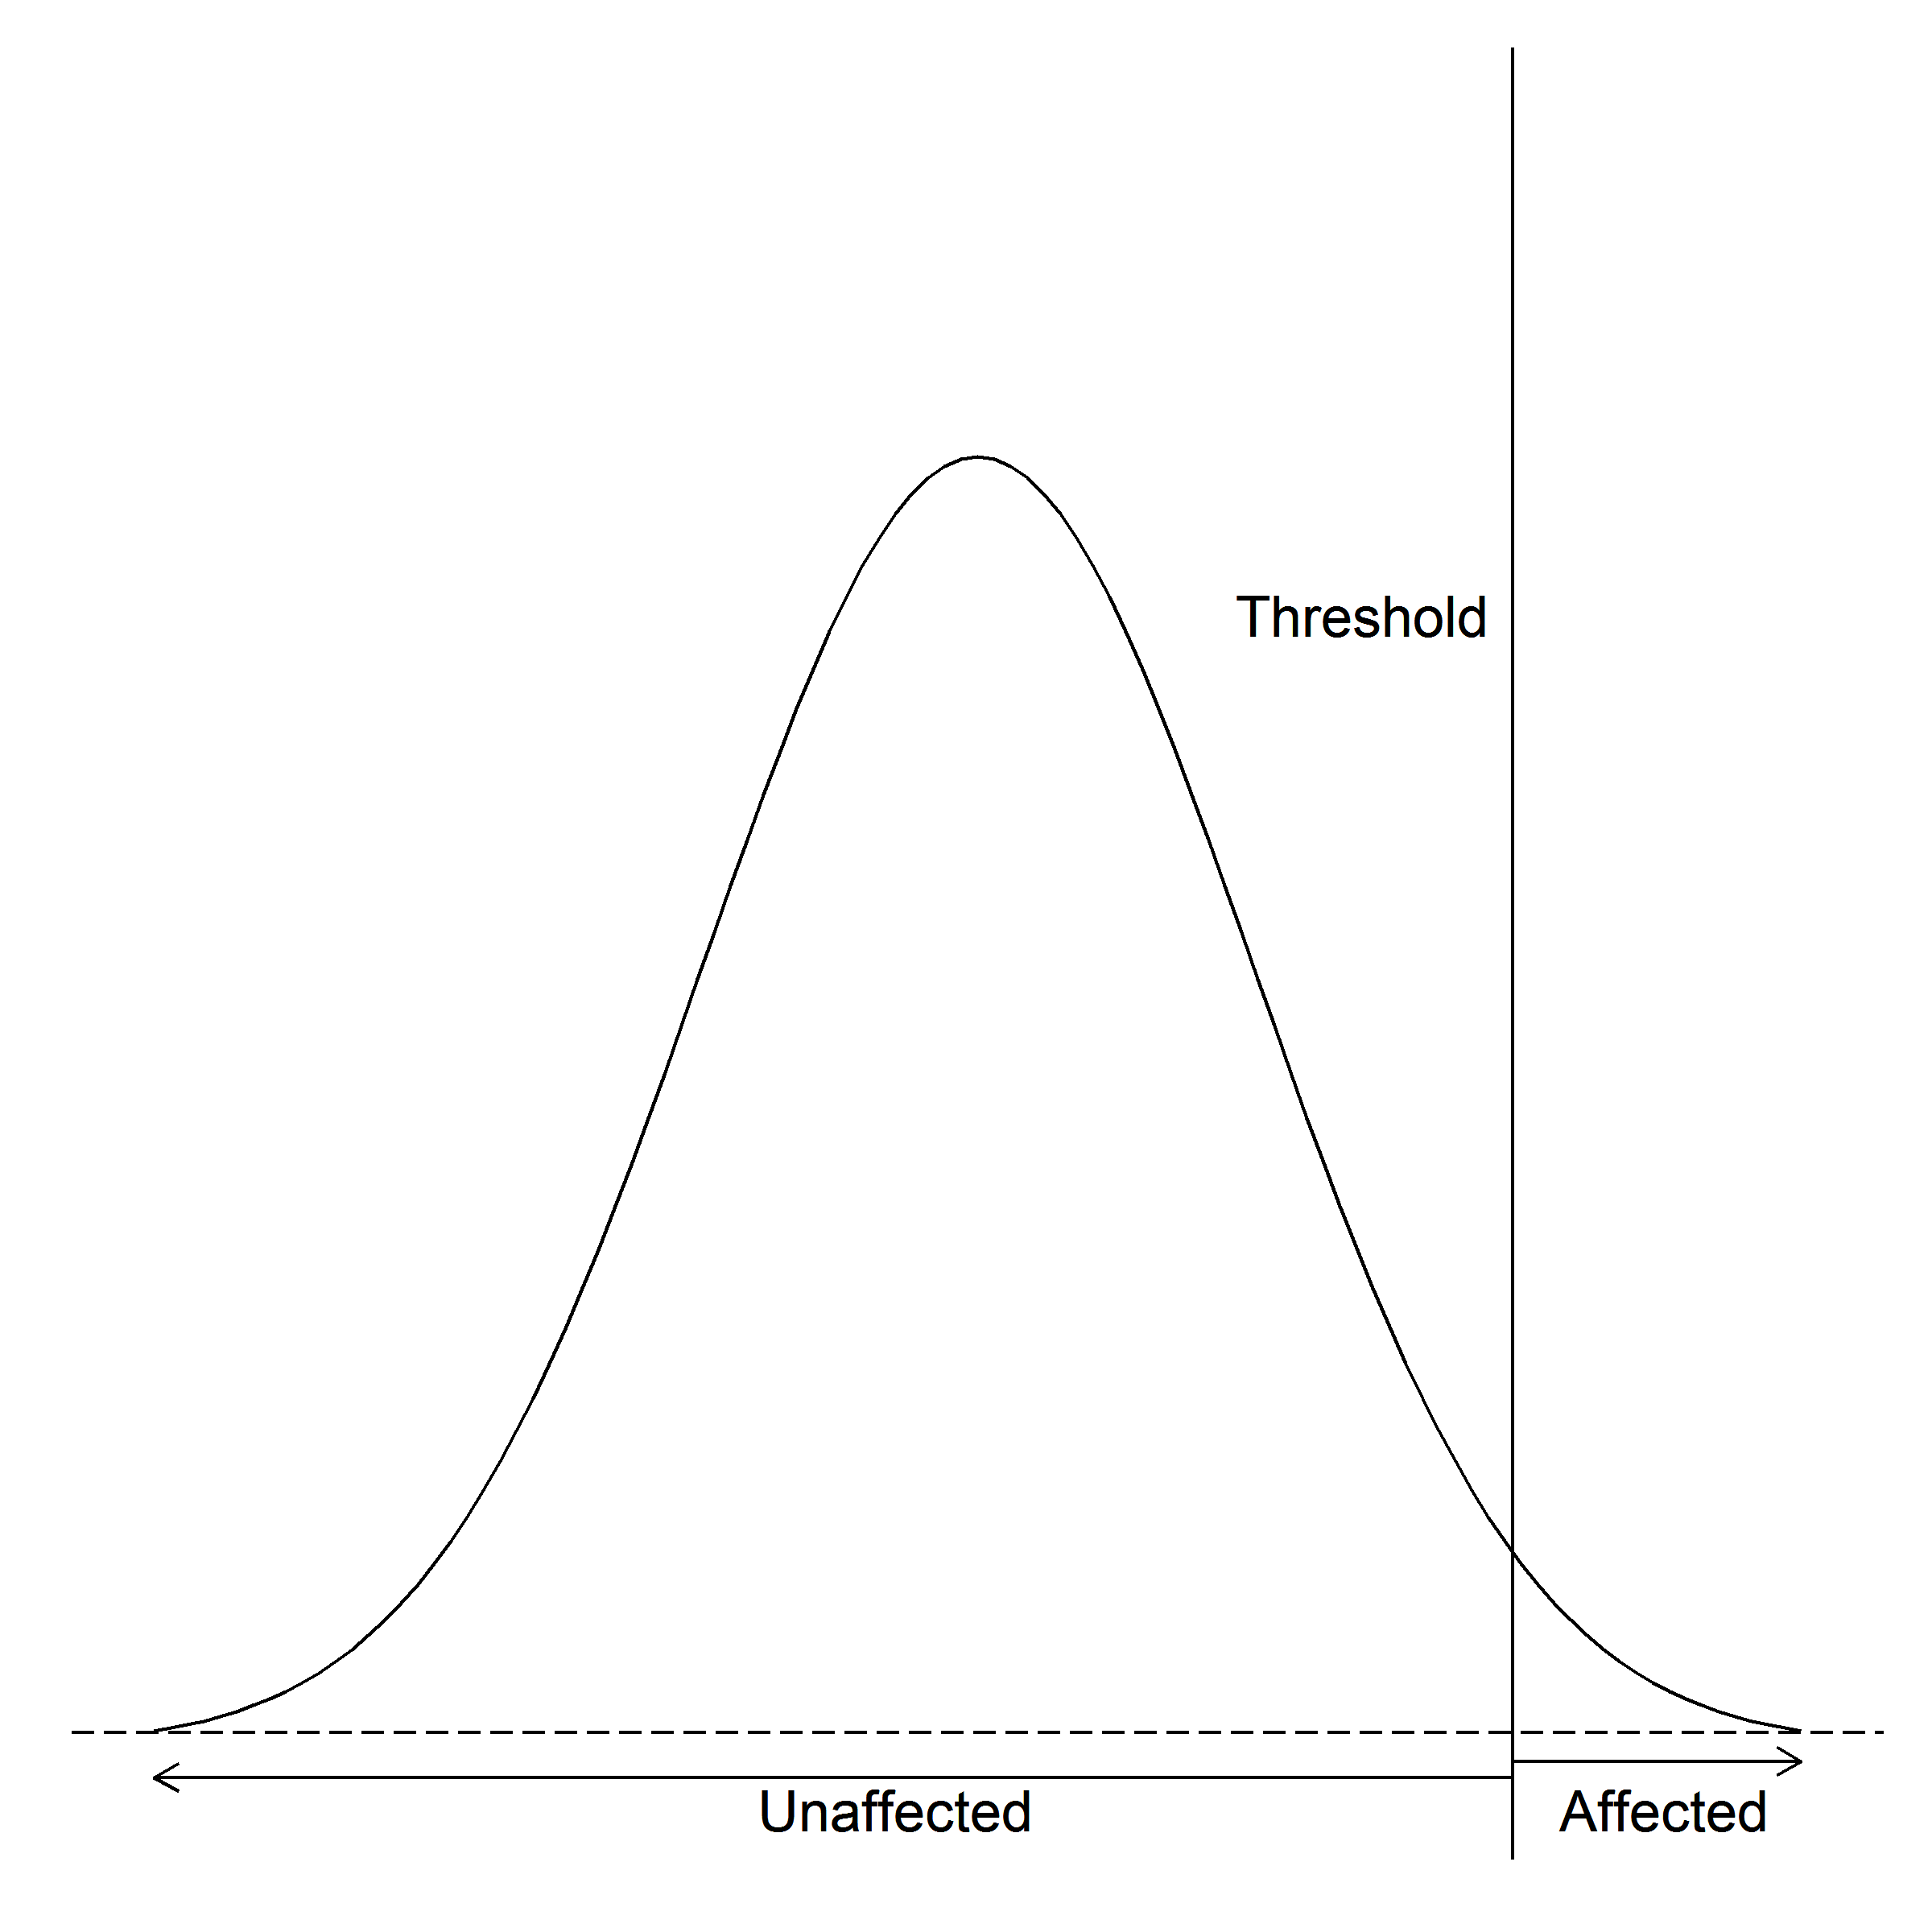
\includegraphics[width=0.5\textwidth]{figure/liability.png}
	\caption[Liability Threshold Model]{
		The liability threshold model.
		Only when an individual has a liability above the liability threshold will he/she be affected.
	}
	\label{fig:liability}
\end{figure}
One can then estimate the heritability of the discontinuous traits by comparing the mean liability of the general population to that of the relatives of the affected individuals.	
For example, considering a single threshold model of a dichotomous trait, where 
\begin{align}
T_G &= \text{Liability threshold of the general population}\notag\\
T_R &= \text{Liability threshold of relatives of the index case} \notag\\
q_G &= \text{Prevalence in the general population}\notag\\
q_R &= \text{Prevalence in relatives of the index case}\notag\\
L_a &= \text{Mean Liability of the index case} \notag
\end{align}
by assuming both the liability distribution of the general population and the relative of the index case follow the standard normal distribution, the two distributions can be aligned with respect to $T_G$ and $T_R$. 
The mean liability of the index case $L_a$ can then be calculated as $L_a=\frac{z_G}{q_G}$ where $z_G$ is the value of the density function of the standard normal distribution at the liability threshold $T_G$.
The regression of relatives' liability on the liability of the index case can be expressed as
\begin{align}
\beta &= \frac{T_G-T_R}{L_a}
\label{eq:liability}
\end{align}

Thus, by applying \cref{eq:liability} to \cref{eq:finalNarrow},
\begin{align}
h^2 =\frac{T_G-T_R}{rL_a}
\end{align}

\subsection{Adoption Study}
One key limitation of \cref{eq:finalNarrow} is its inability to discriminate the genetic factors from the shared environmental factors.
Relatives can share not only the additive genetic effect of alleles, but also some of the environmental factors such as diet and socio-economic status. 

Adoption studies are one of the classic tools for discriminating the effect of additive genetic factors from the effects of environmental factors. 
In adoption studies, the child is separated from their family soon after birth, thus minimized the effect of shared environmental factors.
Any resemblance between the parent and offspring should be driven primarily by the shared genetic factors.

In the classical adoption study carried out by \citet{HESTON1966} in 1966, 47 individuals who were born to schizophrenic mothers during the period from 1915 to 1947 were collected. 
The child were separated from their mother within three days of birth and sent to a foster family. 
50 matched controls were also recruited in this study.
An increased risk of \scz\ was observed in individuals born to schizophrenic mothers when compared to the controls, even-though they were separated from their mother early on.
This provide strong support for \scz\ as a genetic disorder. 

\subsection{Twin Studies}
Despite the usefulness of adoption studies, collection of adoption data are extremely difficult. 
Moreover, adoption studies cannot control the prenatal environment such as alcohol abuse and malnutrition during pregnancy.
For example, a high comorbidity of alcohol use disorders and \scz\ was observed \citep{boyd1984,drake1990}. 
High consumption level of alcohol during pregnancy may bring about long-term alterations in nervous system functioning of the offspring \citep{garrett2014brain}.
This increased risk of \scz\ in the offspring might therefore be an artifact of the alcohol abuse of the mother. 

Alternatively, twin studies, which utilize the genetic relationship between \gls{mz} and \gls{dz} twins, can be performed to estimate the heritability of the target trait.

By definition, the common environmental factors ($C$) is the same for the twins whereas the non-shared environmental factors ($E$) is unique to each individual.
For \gls{mz} twins, both the additive ($A$) and non-additive ($D$) genetic factors are shared between the siblings. 
On the other hand, only $\frac{1}{2}$ of the additive genetic factors and $\frac{1}{4}$ of the non-additive genetic factors are shared among the \gls{dz} twins \citep{rijsdijk2002analytic}.

In view of this, \citet{falconer1996introduction} derived the heritability as
\begin{equation}
h^2 = 2(\rho_{MZ}-\rho_{DZ})
\end{equation}
where $\rho_{MZ}$ and $\rho_{DZ}$ are the phenotype correlation between the \gls{mz} twins and \gls{dz} twins respectively.
However, if assortative mating occurs in the population, the additive genetic factors shared between the \gls{dz} twins might be higher than $\frac{1}{2}$, thus leading to a underestimation of the heritability.
Nonetheless, twin studies can be served as the first step in the study of genetic architecture and provide vital understanding of the trait.

By combining Falconer's formula and the concept of liability threshold model, \citet{Gottesman1967} estimated that the heritability of \scz\ to be $>60\%$ based on previously collected twin data.
This provides strong evidence that the genetic variation contributes more to the variance of \scz.

The result was further supported by one of the landmark meta-analysis study conducted by \citet{Sullivan2003}.
Based on data obtained from 12 published \scz\ twin studies, \citet{Sullivan2003} found much contribution from genetics on the liability of \scz\ ($81\%$, \gls{ci}=$73\%-90\%$).
Furthermore, in the large scale population based studies performed by \citet{Lichtenstein2009}, the genetic contribution to \scz\ was found to be $64\%$.
Together, these results provide strong support for \scz\ as a genetic disorder. 

\section{Schizophrenia Genetics}
Although \scz\ is highly heritable, little is known about the disease mechanism of \scz\ and the genetic complexity of the disorder. 
It was observed that the lifetime morbid risk of \gls{mz} twins were only $48\%$ (\cref{fig:lifeMRscz}), suggesting that it is unlikely for \scz\ to follow the Mendelian framework \citep{Gottesman1967,Gottesman1982,gottesman1991schizophrenia}.	
\begin{figure}[t]
	\centering
	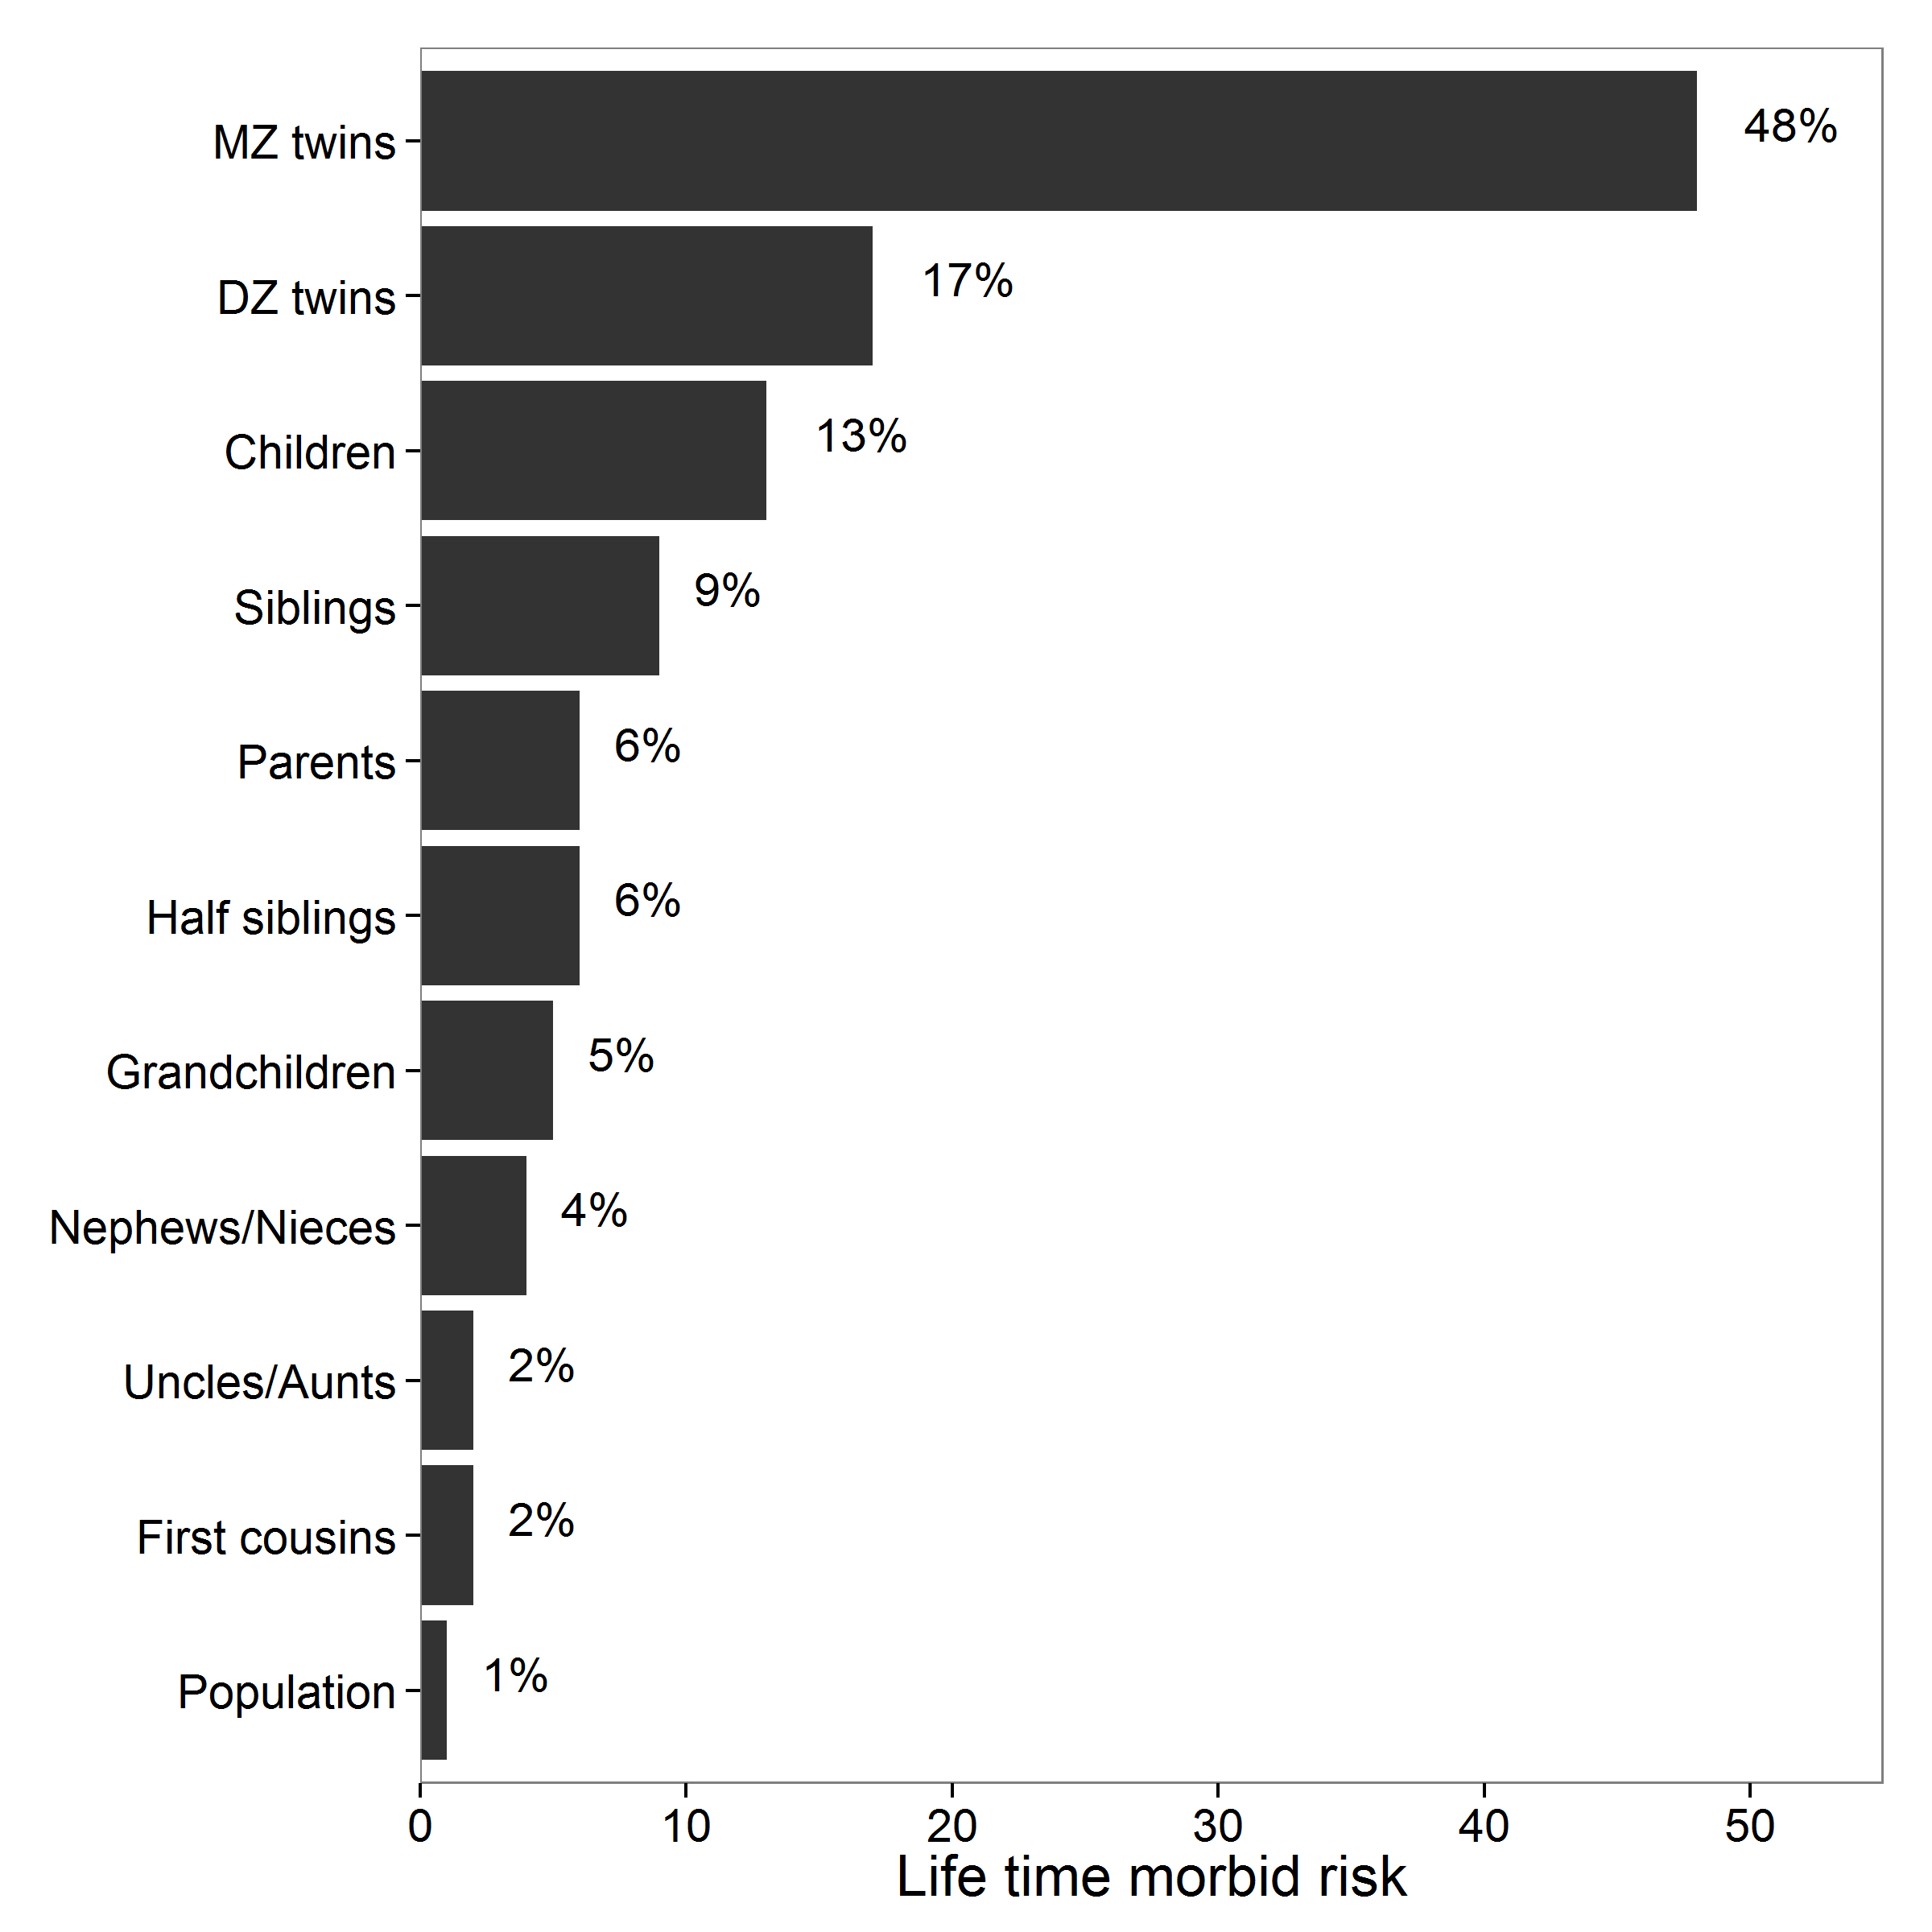
\includegraphics[width=0.6\textwidth]{figure/lifeTimeMorbidRisk.png}
	\caption[Lifetime morbid risks of \scz\ in various classes of relatives of a proband]{Lifetime morbid risks of \scz\ in various classes of relatives of a proband.
It was noted that the morbid risk of \gls{mz} twins was only $48\%$, much lower than one would expect if \scz\ follows a Mendelian pattern.
	Reproduced with permission from journal \citep{Riley2006}. \label{fig:lifeMRscz}}
\end{figure}
	
In view of this, \citet{Gottesman1967} proposed that \scz\ might follow a polygenic model, where the disease phenotype were determined by the additive effects from multiple genes.
	
By comparing the observed lifetime morbid risk and the expected risk from different models, \citet{Risch1990} proposed that the causal variants of \scz\ are more likely to have a risk less than 2 with no loci with risk larger than 3, suggesting a relatively small effect size.
Large sample size are therefore required to detect these susceptibility loci through linkage studies \citep{Risch1990}.

As genetic data from large, multi-generational pedigrees with both affected and unaffected individuals are difficult to recruit, it is challenging for linkage studies to collect adequate samples. 
Thus early linkage studies of \scz\ results in inconsistent findings \citep{Harrison2005}.
Other methods are therefore required to identify the susceptibility loci of \scz.

\subsection{The Human Genome Project and HapMap Project}
\glsreset{SNP}
\glsreset{LD}
In 1990, the Human genome project was initiated, aiming at constructing the first physical map of the human genome at per nucleotide resolution \citep{Lander2001}.
The completion of the human genome project has opened up a new era of genetic research, allowing researchers to identify \glspl{SNP}, which is one of the major source of genetic variation in the human genome.

Soon after the completion of the human genome project, the HapMap Project was initiated \citep{Consortium2005}, aiming to provide a genome-wide database of common human sequence variation such as \glspl{SNP} with \gls{maf} $\ge0.05$.

More importantly, the HapMap Project provided a detailed \gls{LD} map of the human genome.
\gls{LD} is the non-random correlation of genotypes between 2 genetic loci. 
\glspl{SNP} in high \gls{LD} are usually observed together in the human genome.
When a large amount of \glspl{SNP} are in high \gls{LD}, a \gls{LD} block is formed.
By performing association testing on \glspl{SNP} representing majority of the information within the \gls{LD} block (``tagging''), genome-wide association can be performed.
This is the fundamental concept of \gls{GWAS}, which is now extensively used in genetic researches.

\subsection{Genome Wide Association Study}
In \gls{GWAS}, genome-wide genotyping array are commonly used to systematically detect genetic variants such as \gls{SNP} and \gls{cnv} in genome-wide scale.
For quantitative traits, the association between the trait and frequency of the variants are calculated using methods such as linear regression.
On the other hand, for dichotomous traits such as \scz, the frequency of the variants are compared between the case and control samples using chi-square test or logistic regression.

However, when a large number of \glspl{SNP} were tested, the frequency of type I error increases \citep{Peters2010}.
Most importantly, even in the scenario where only one \gls{SNP} was tested, the number of potential comparison can still be high \citep{gelman2016statistical}.
Again, this may result in large type I error.   
Thus, multiple testing correction is vital in the analysis of \gls{SNP} association.

The simplest method for the correction of \gls{GWAS} is to use the genome wide threshold (p-value $\le5\times10^{-8}$), where only \glspl{SNP} with p-value less then the genome wide threshold are considered to be significant in \gls{GWAS}.
Another possible method to decide the significant threshold is to consider the ``effective number'' of tests \citep{Li2011}, which reduced the genome-wide threshold according to the \gls{LD} structure.

Finally, when designing a \gls{GWAS}, the magnitude of effect, sample size, and required level of statistical significance (the false-positive, or type I, error rate) are all important factors determining the detection power of the \gls{GWAS} \citep{Purcell2003}.
Similar to linkage studies, a larger sample size are required to identify susceptible loci with a smaller effect. 

\subsubsection{The Success of Psychiatric Genomic Consortium} 
Due to the relatively small sample size, early \gls{GWAS} in \scz\ were largely disappointing, where no robust genetic markers associated with \scz\ were identified. 

To overcome the problem of sample size, large consortium were formed such that genetic data from different research groups can be combined and analyzed.
Finally, in 2014, the \Scz\ Working group of the \gls{pgc} has conducted a multi-stage \scz Genome-Wide Meta Analysis of up to 36,989 \scz\ samples and 113,075 controls \citep{Ripke2014}.
A total of 128 linkage-disequilibrium-independent \glspl{SNP} were found to exceeded the genome-wide significance (p-value $\le 5\times10^{-8}$), correspond to 108 independent genetic loci.
75\% of these loci contain protein coding genes and a further 8\% of these loci were within 20 \gls{kb} of a gene. 
It was found that genes involved in glutamatergic neurotransmission (e.g. \textit{GRM3}, \textit{GRIN2A} and \textit{GRIA1}), synaptic plasticity and genes encoding the voltage-gated calcium channel subunits (e.g. \textit{CACNA1C}, \textit{CACNB2} and \textit{CACNA1I}) were among the genes associated within these loci.
Moreover, associations were significantly enriched at enhancers active in brain and in tissues with important immune functions (\cref{fig:pgcEnrich}) \citep{Ripke2014}.

\begin{figure}
	\centering
	\caption[Enrichment of enhancers of SNPs associated with Schizophrenia]{Enrichment of enhancers of SNPs associated with \scz. 
		It was observed that the largest enrichment were in cell lines related to the brain and in tissues with important immune functions. 
		Graphs reproduced with permission from the journal \citep{Ripke2014}.}
	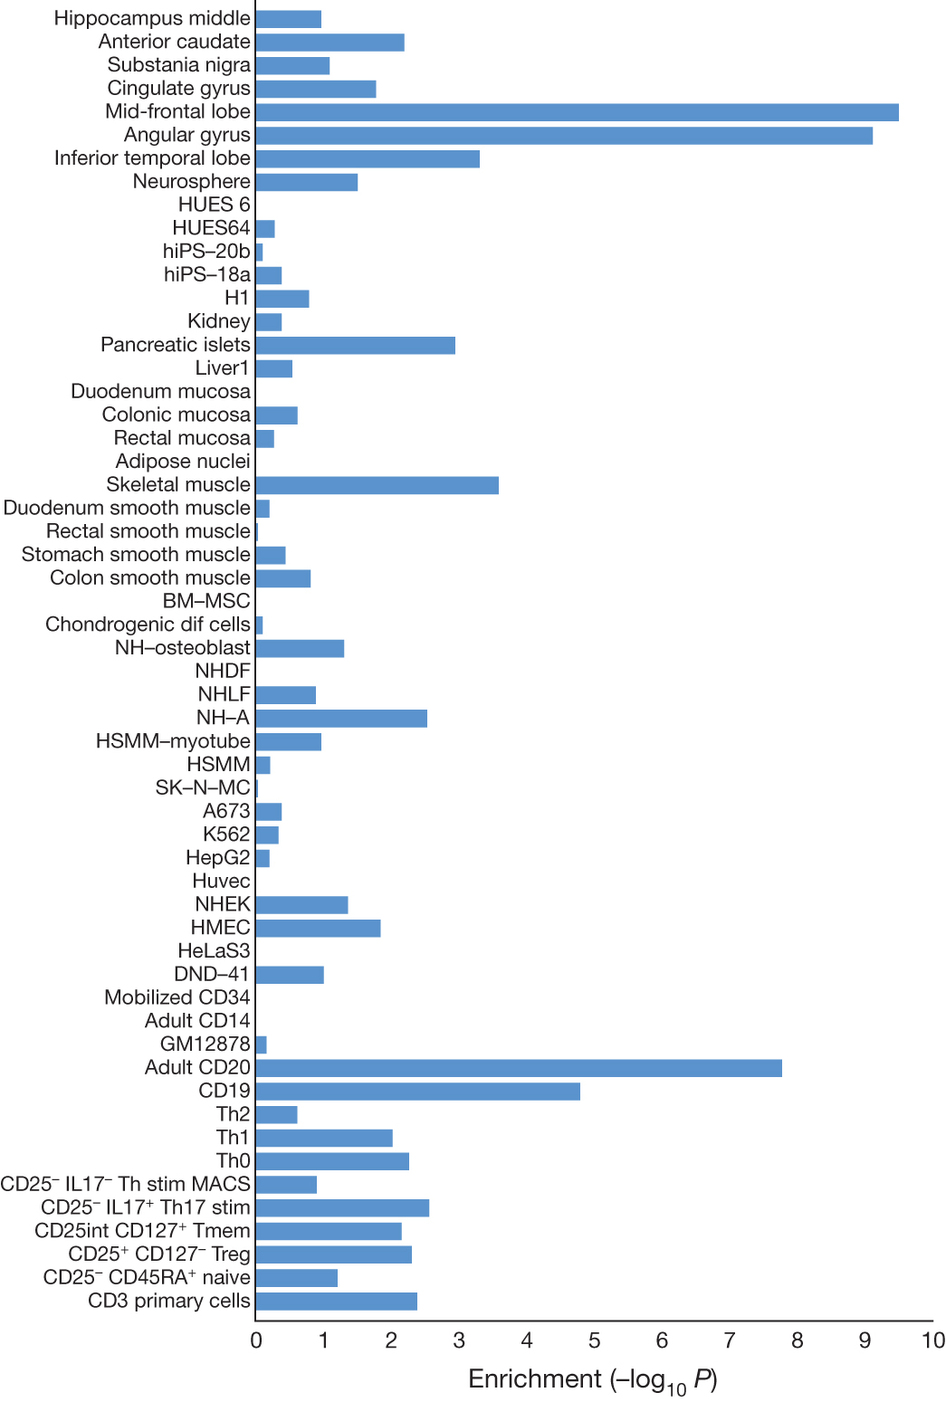
\includegraphics[height=\textwidth]{figure/pgc_enrichment_tissue.jpg}
	\label{fig:pgcEnrich}
\end{figure}

The enrichment of immune related enhancers remains significant even after the removal of \gls{mhc} region from the analysis, suggesting that the significance association of the immune system with \scz\ is not driven only by the \gls{mhc} region.
Considering the role of immune system in neural development \citep{Zhao1998,Deverman2009}, perturbation in the immune system is likely to disrupt the brain development.
Therefore, the immune system might have an important role in the etiology of \scz.

Given the success of \gls{pgc} \scz\ \gls{GWAS}, it is interesting to investigate the relative contribution of common variants, which are captured in the \gls{GWAS}, to the genetic predisposition of \scz.
This will provide vital information as to whether other genetic variations such as rare mutations and methylation are also important. 

\subsection{Contribution of Common SNPs}
By imposing a stringent genome-wide significant threshold to the results of \gls{GWAS}, the Type I error can be reduced. 
However, real associations with a small effect size might be filtered out through multiple testing correction.
Therefore, to estimate the true contribution of common \glspl{SNP} to a trait (\gls{SNP}-heritability), it is necessary to consider all the \glspl{SNP} in the estimation.

\subsubsection{Genome-wide Complex Trait Analysis}
Currently, the most popular algorithm for the estimation of \gls{SNP}-heritability is \gls{gcta}, which utilize information from the \gls{grm} \citep{Yang2011}.
The \gls{grm} represents the genetic relationship between all individuals within the \gls{GWAS}.
The genetic relationship between individual $j$ and $k$ can be estimated as 
\begin{equation}
A_{jk} = \frac{1}{N}\sum^N_{i=1}\frac{(x_{ij}-2p_i)(x_{ik}-2p_i)}{2p_i(1-p_i)}
\end{equation}
where $x_{ij}$ is the number of copies of the reference allele for the $i^{th}$ \gls{SNP} of the $j^{th}$ individual and $p_i$ is the frequency of the reference allele.
Because genotypes are usually code as 0, 1 or 2 (homozygous reference, heterozygous and homozygous alternative respectively), one can model the distribution of genotype using the binomial distribution.
Therefore, the expected mean and variance of genotype $i$ is $2p_i$ and $2p_i(1-p_i)$ respectively, and the \gls{grm} can be represented as $A_{jk} = \frac{1}{N}\sum^N_{i=1}z_{ij}z_{ik}$, where $z_{ij}$ is the standardized genotype for the $i^{th}$ \gls{SNP} of the $j^{th}$ individual.

Using the information from the \gls{grm}, \citet{Yang2011} fitted the effects of all the \glspl{SNP} as random effects in a \gls{mlm}
\begin{align}
\boldsymbol{y} &= \boldsymbol{X\beta}+\boldsymbol{g}+\epsilon\\
\mathrm{Var}(\boldsymbol{y}) &= \boldsymbol{A}\sigma_g^2+\boldsymbol{I}\sigma_\epsilon^2
\label{eq:gctaEq}
\end{align}
where $\boldsymbol{y}$ is an $n\times 1$ vector of phenotypes with $n$ samples, $\boldsymbol{\beta}$ is a vector of fixed effects such as sex and age, $\boldsymbol{g}$ is an $n\times 1$ vector of the total genetic effects of the individuals, $\sigma_g^2$ is the variance explained by all the \glspl{SNP} and finally, $\sigma_\epsilon^2$ is the variance explained by residual effects.

By fitting the effects of \emph{all} \glspl{SNP} as random effects in a \gls{mlm}, a single parameter can be estimated, i.e. the variance explained by all \glspl{SNP} or \gls{SNP}-heritability.
Based on \cref{eq:gctaEq}, \citet{Yang2011} implemented the \gls{reml} using the average information algorithm to provide an unbiased estimates of $\sigma_g^2$ and $\sigma_\epsilon^2$.
The \gls{SNP}-heritability of the trait can then be defined as $\frac{\sigma_g^2}{\sigma_g^2+\sigma_e^2}$.
	
\citet{Yang2010a} were able to estimate the variance in height explained by \gls{GWAS} \glspl{SNP}  to be around 45\%, much larger than previously reported 5\%.
However, the estimate was still less than 80\%, which is the expected heritability of height.
\citet{Yang2010a} hypothesized that one possible source of ``missing heritability'' might be due to incomplete \gls{LD} of the \gls{GWAS} chip.
Taken into consideration of incomplete \gls{LD}, \citet{Yang2010a} estimated that the proportion of variance explained by causal variants to be as high as 0.84 with \gls{se} of 0.16, within the range of the expected heritability of height, providing support to their hypothesis.

By far, the biggest limitation of \gls{gcta} is the requirement of individual genotype data to calculate the \gls{grm}.
For studies where only summary statistics are available, e.g. the meta-analysis of \scz, \gls{gcta} analysis cannot be performed.
Therefore, other methods are required. 
	
\subsubsection{\glng{ldsc}}
In large scale \gls{GWAS} studies, a general inflation of summary statistics can sometimes be observed.
The inflation was usually considered to be contributed by the presence of confounding factors such as population stratification, under the assumption that most of the \glspl{SNP} were not associated with the disease.
Therefore, \gls{gc} inflation factor were usually used to control for the inflation in \gls{GWAS} results \citep{Zheng2006}.
	
However, for complex diseases such as \scz, there might be a large number of causal \glspl{SNP}, therefore violating the underlying assumption of \gls{gc}. 
Through careful simulation, \citet{Yang2011b} demonstrated that in the absence of population stratification and other form of technical artifacts, the presence of polygenic inheritance can inflate the summary statistic.
It was observed that the magnitude of inflation was determined by the \emph{heritability}, the \gls{LD} structure, sample size and the number of causal \glspl{SNP} of the trait.

\citet{Bulik-Sullivan2015} noted that the variants in \gls{LD} with a causal variant show an elevation in summary statistic proportional to their \gls{LD} with the causal variant. 
Therefore, the more \glspl{SNP} that are in \gls{LD} with the index \gls{SNP}, the higher the likelihood for the index \gls{SNP} to tag the causal variant. 
However, inflation in summary statistic resulting form cryptic relatedness and population stratification will not correlate with \gls{LD}.
Therefore, \citet{Bulik-Sullivan2015} developed the \gls{LD} score, where the \gls{LD} score of a \gls{SNP} $j$ is defined as the sum of $r^2$ of $k$ neighboring \glspl{SNP} within a 1 \gls{cm} window:
\begin{equation}
l_j = \sum_kr^2_{jk}
\label{eq:ldScore}
\end{equation}

The expected $\chi^2$s association of \gls{SNP}$_j$ with the trait can then be defined as a function of the \gls{LD} score ($l_j$), the number of samples ($N$), the number of \glspl{SNP} in the analysis ($M$) and most importantly, the \gls{SNP} heritability ($h^2$):
\begin{equation}
\mathrm{E}[\chi^2_j | l_j] = \frac{Nh^2}{M}l_j+1
\label{eq:fixedLDSC}
\end{equation}

Alternatively, if confounding factors are present in the study (e.g. population stratification), \cref{eq:fixedLDSC} can be defined as
\begin{equation}
\mathrm{E}[\chi^2_j | l_j] = \frac{Nh^2}{M}l_j+Na+1
\label{eq:fullLDSC}
\end{equation}
where $a$ is the contribution of the confounding bias.

By considering \cref{eq:fullLDSC} as a regression model, \citet{Bulik-Sullivan2015} observed that the contribution of common variants (the \gls{SNP} heritability $h^2$) is the slope of the regression, whereas the intercept minus one will represent the mean contribution of the confounding bias, such as population stratification. 
Using \cref{eq:fullLDSC}, \citet{Bulik-Sullivan2015} implemented the \gls{ldsc} to delineate the contribution from confounding factors and common genetic variants.

To assess the performance of \gls{ldsc}, \citet{Bulik-Sullivan2015} performed a number of controlled simulation.
First, they simulated polygenic traits without any confounding factors. 
The result shows that the average intercept estimated by \gls{ldsc} was closed to one, correctly suggest the absence of confounding factors.
Moreover, the heritability estimates provided by \gls{ldsc} were unbiased for all simulated conditions. 
Only when the number of causal variants was small did the standard error of the \gls{ldsc} estimates become very large.
Similarly, when non-genetic trait was simulated with only confounding factors such as population stratification, the intercepts estimated by \gls{ldsc} were approximately equal to the \gls{gc} inflation factor, with only a small positive bias in the regression slope.
Most importantly, when polygenic traits with confounding factors were simulated, the intercepts estimated by \gls{ldsc} were approximately equal to the mean $\chi^2$ statistics among the null \glspl{SNP}.
This provide strong evidence that the \gls{LD} score regression can partition the inflation in test statistics even in the presence of both bias and polygenicity.

Following the success of their simulation, \citet{Bulik-Sullivan2015} utilized \gls{ldsc} to estimate the \gls{SNP} heritability of \scz\ using the summary statistics from the \gls{pgc} \scz\ \gls{GWAS} \citep{Ripke2014}.
The estimated \gls{SNP} heritability of \scz\ is around 0.555 with standard error of 0.008 after adjusting for ascertainment bias. 
Comparing the \gls{SNP} heritability estimated with the heritability estimated from the population study (64\% \citep{Lichtenstein2009}) and the twin studies (81\% \citep{Sullivan2003}), it seems as if the common variants have accounted for most if not all of the heritability of \scz.

\subsubsection{Partitioning of Heritability}
Other than the estimation of \gls{SNP} heritability, \gls{ldsc} also allows for the partitioning of heritability into different pathways, which can be used for functional enrichment analysis. 

Traditionally, functional enrichment analysis in \gls{GWAS} only consider significant \glspl{SNP}. 
However, \glspl{SNP} with small effect size that do not reach genome-wide significance threshold might be filtered out.
For example, in 2013, only 13 risk loci were detected using 13,833 \scz\ samples and 18,310 controls \citep{Ripke2013}. 
Yet when the sample size increased to 34,241 \scz\ samples and 45,604 controls in 2014, 108 risk loci were identified \citep{Ripke2014}.
Thus, only when sample size are larger can those risk loci with a smaller effect size to be able to reach the genome-wide significance threshold.
By filtering the insignificant loci, the functional enrichment analysis might loses power. 

On the other hand, \gls{ldsc} utilize the summary statistic of all the \glspl{SNP} included in the \gls{GWAS} when estimating the association of a functional category with the trait.
Specifically, \cref{eq:fullLDSC} modified into
\begin{equation}
\mathrm{E}[\chi^2_j] = N\sum_C\tau_Cl(j,C)+Na+1
\label{eq:partitionH}
\end{equation}
with $\frac{h^2}{M}l_j$ substituted by $\sum_C\tau_Cl(j,C)$ where $l(j,C)$ is the \gls{LD} Score of \gls{SNP} $j$ with respect to category $C$ and $\tau C$ is the per-\gls{SNP} heritability in category $C$.

By applying \cref{eq:partitionH} to the summary statistics from the \gls{pgc} \scz\ \gls{GWAS}, \citet{Finucane2015} found that brain cell types and immune related cell types were most enriched in \scz.
Of all the functional categories, H3K4me3 mark in the fetal brain (\cref{tab:cellTypeScz}) was the most enriched in \scz.
As H3K4me3 is mostly linked to active promoters, genes activated in fetal brain (e.g. genes related to brain development) are therefore likely to be associated with \scz, supporting the idea of \scz as a neuro-developmental disorder. 

	\begin{singlespace}
		\begin{longtable}{p{6cm}rrr}
			%\begin{tabular}{rrrr}
			\toprule
			Cell type & cell-type group & Mark  & P-value \\
			\midrule
			Fetal brain** & CNS   & H3K4me3 & $3.09\times 10^{-19}$ \\
			Mid frontal lobe** & CNS   & H3K4me3 & $3.63\times 10^{-15}$ \\
			Germinal matrix** & CNS   & H3K4me3 & $2.09\times 10^{-13}$ \\
			Mid frontal lobe** & CNS   & H3K9ac & $5.37\times 10^{-12}$ \\
			Angular gyrus** & CNS   & H3K4me3 & $1.29\times 10^{-11}$ \\
			Inferior temporal lobe** & CNS   & H3K4me3 & $1.70\times 10^{-11}$ \\
			Cingulate gyrus** & CNS   & H3K9ac & $5.37\times 10^{-11}$ \\
			Fetal brain** & CNS   & H3K9ac & $5.75\times 10^{-11}$ \\
			Anterior caudate** & CNS   & H3K4me3 & $2.19\times 10^{-10}$ \\
			Cingulate gyrus** & CNS   & H3K4me3 & $4.57\times 10^{-10}$ \\
			Pancreatic islets** & Adrenal/Pancreas & H3K4me3 & $2.24\times 10^{-09}$ \\
			Anterior caudate** & CNS   & H3K9ac & $3.16\times 10^{-9}$ \\
			Angular gyrus** & CNS   & H3K9ac & $4.68\times 10^{-9}$ \\
			Mid frontal lobe** & CNS   & H3K27ac & $7.94\times 10^{-9}$ \\
			Anterior caudate** & CNS   & H3K4me1 & $1.20\times 10^{-8}$ \\
			Inferior temporal lobe** & CNS   & H3K4me1 & $3.72\times 10^{-8}$ \\
			Psoas muscle** & Skeletal Muscle & H3K4me3 & $4.17\times 10^{-8}$ \\
			Fetal brain** & CNS   & H3K4me1 & $6.17\times 10^{-8}$ \\
			Inferior temporal lobe** & CNS   & H3K9ac & $9.33\times 10^{-8}$ \\
			Hippocampus middle** & CNS   & H3K9ac & $9.33\times 10^{-7}$ \\
			Pancreatic islets** & Adrenal/Pancreas & H3K9ac & $1.62\times 10^{-6}$ \\
			Penis foreskin melanocyte primary** & Other & H3K4me3 & $2.09\times 10^{-6}$ \\
			Angular gyrus** & CNS   & H3K27ac & $2.34\times 10^{-6}$ \\
			Cingulate gyrus** & CNS   & H3K4me1 & $2.82\times 10^{-6}$ \\
			Hippocampus middle** & CNS   & H3K4me3 & $2.82\times 10^{-6}$ \\
			CD34 primary** & Immune & H3K4me3 & $4.68\times 10^{-6}$ \\
			Sigmoid colon** & GI    & H3K4me3 & $5.01\times 10^{-6}$ \\
			Fetal adrenal** & Adrenal/Pancreas & H3K4me3 & $6.31\times 10^{-6}$ \\
			Inferior temporal lobe** & CNS   & H3K27ac & $8.32\times 10^{-6}$ \\
			Peripheralblood mononuclear primary** & Immune & H3K4me3 & $9.33\times 10^{-6}$ \\
			Gastric** & GI    & H3K4me3 & $1.17\times 10^{-5}$ \\
			Substantia nigra* & CNS   & H3K4me3 & $1.95\times 10^{-5}$ \\
			Fetal brain* & CNS   & H3K4me3 & $2.63\times 10^{-5}$ \\
			Hippocampus middle* & CNS   & H3K4me1 & $3.31\times 10^{-5}$ \\
			Ovary* & Other & H3K4me3 & $6.46\times 10^{-5}$ \\
			CD19 primary (UW)* & Immune & H3K4me3 & $7.08\times 10^{-5}$ \\
			Small intestine* & GI    & H3K4me3 & $8.51\times 10^{-5}$ \\
			Lung* & Cardiovascular & H3K4me3 & $1.17\times 10^{-4}$ \\
			Fetal stomach* & GI    & H3K4me3 & $1.29\times 10^{-4}$ \\
			Fetal leg muscle* & Skeletal Muscle & H3K4me3 & $1.51\times 10^{-4}$ \\
			Spleen* & Immune & H3K4me3 & $1.70\times 10^{-4}$ \\
			Breast fibroblast primary* & Connective/Bone & H3K4me3 & $2.04\times 10^{-4}$ \\
			Right ventricle* & Cardiovascular & H3K4me3 & $2.14\times 10^{-4}$ \\
			CD4+ CD25- Th primary* & Immune & H3K4me3 & $2.19\times 10^{-4}$ \\
			CD4+ CD25- IL17- PMA Ionomycin stim MACS Th sprimary* & Immune & H3K4me1 & $2.19\times 10^{-4}$ \\
			CD8 naive primary (UCSF-UBC)* & Immune & H3K4me3 & $2.24\times 10^{-4}$ \\
			Pancreas* & Adrenal/Pancreas & H3K4me3 & $2.34\times 10^{-4}$ \\
			CD4+ CD25- Th primary* & Immune & H3K4me1 & $2.75\times 10^{-4}$ \\
			CD4+ CD25- CD45RA+ naive primary* & Immune & H3K4me1 & $2.75\times 10^{-4}$\\
			Colonic mucosa* & GI    & H3K4me3 & $3.24\times 10^{-4}$ \\
			Right atrium* & Cardiovascular & H3K4me3 & $3.31\times 10^{-4}$ \\
			Fetal trunk muscle* & Skeletal Muscle & H3K4me3 & $3.39\times 10^{-4}$ \\
			CD4+ CD25int CD127+ Tmem primary* & Immune & H3K4me3 & $3.47\times 10^{-4}$ \\
			Substantia nigra* & CNS   & H3K9ac & $3.63\times 10^{-4}$ \\
			Placenta amnion* & Other & H3K4me3 & $4.17\times 10^{-4}$ \\
			Breast myoepithelial* & Other & H3K9ac & $5.50\times 10^{-4}$ \\
			CD8 naive primary (BI)* & Immune & H3K4me1 & $5.75\times 10^{-4}$ \\
			Substantia nigra* & CNS   & H3K4me1 & $6.61\times 10^{-4}$ \\
			Cingulate gyrus* & CNS   & H3K27ac & $7.94\times 10^{-4}$ \\
			CD4+ CD25- CD45RA+ naive primary* & Immune & H3K4me3 & $8.71\times 10^{-4}$ \\
			\bottomrule
			%\end{tabular}%
			\caption[Enrichment of Top Cell Type of Schizophrenia]{Enrichment of Top Cell type of Schizophrenia.
				* = significant at False Discovery Rate $<$ 0.05.
				** = significant at p $<$ 0.05 after correcting for multiple hypothesis. 
				Reproduce with permission from Journal.\citep{Finucane2015}}
			\label{tab:cellTypeScz}%
		\end{longtable}%
	\end{singlespace}	

\subsection{Contribution of Other Genetic Variants}
\glsreset{cnv}
Although the estimated \gls{SNP} heritability of \scz\ by \citet{Bulik-Sullivan2015} suggest common \glspl{SNP} to be the major contributor to the heritability of \scz, other variants, such as \gls{cnv} have been found to be associated with \scz.

\subsubsection{Copy Number Variation}
\gls{cnv} are classified as segment of DNA that is 1 \gls{kb} or larger, and is present at a different copy number when compared to the reference genome, usually in the form of insertion, deletion or duplication \citep{Feuk2006}.
Due to the length of \gls{cnv}, these variants might contain the entire genes and their regulatory regions, which might contribute to significant phenotypic differences \citep{Feuk2006}.
	
Recently, \citet{Szatkiewicz2014} conducted a \gls{GWAS} for \gls{cnv} association with \scz\ using the Swedish national sample (4,719 \scz\ samples and 5,917 controls).
A number of risk \glspl{cnv} such as 16p11.2 duplications, 22q11.2 deletions, 3q29 deletions and 17q12 duplications were identified.
In general, \glspl{cnv} associated with \scz\ are rare ($\le12$ in 4,719 samples \citep{Szatkiewicz2014}) and have a relative large effect (e.g. odd ratio $>2$ \citep{Szatkiewicz2014,Walsh2008}).

\citet{Szatkiewicz2014} also performed the gene set enrichment analysis and they found that calcium ion channel signaling and binding partners of the fragile X mental retardation protein are enriched by \gls{cnv} observed in the schizophrenic samples \citep{Szatkiewicz2014}.

Similar pathways were also found to be enriched with structure variants in schizophrenic samples in a separate study conducted by \citet{Walsh2008}.
Pathways important for brain development, including neuregulin signaling, extracellular signal-regulated kinase/\gls{mapk} signaling, synaptic long-term potentiation, axonal guidance signaling, integrin signaling, and glutamate receptor signaling were all found to be significantly overrepresented with structural variants found in schizophrenic samples.

\subsubsection{Rare Single Nucleotide Mutation}
In addition to \gls{cnv}, there are also evidence of an increased burden of rare variants in \scz\  \citep{purcell2014polygenic}. 
By sequencing the exome of 2,536 \scz\ cases and 2,543 normal controls,  \citet{purcell2014polygenic} identified a common missense allele on \textit{CCHCR1} in the \gls{mhc} region to be associated with \scz.
Although none of the genes showed a significant burden of rare mutation in \scz\ cases, a significant increased burden of rare nonsense and disruptive variants was observed in gene sets such as voltage-gated calcium ion channel, genes affected by \textit{de novo} mutations in \scz\ \citep{Fromer2014} and the postsynaptic density, all of which have been reported to be associated with \scz\ in previous genetic studies \citep{Ripke2014}.

Despite the complexity of \scz, evidence of gene sets enriched by common variants, structural variations, \gls{cnv} and rare variants all converge to the same set of functional pathways, suggesting a common functional pathway is disrupted in \scz\ patients. 
Together, the evidences support for the involvements of genetic variations other than common \glspl{SNP} in the risk of \scz.

\section{Environmental Risk Factors}
In the estimation of heritability of \scz, only the additive genetic factors are considered. 
However, \citet{zuk2012mystery} suggested that failure in accounting for gene-environment interaction might result in ``phantom heritability'' \citep{zuk2012mystery}.
Specifically, presence of the gene-environment interaction can increase the total heritability of a trait.

In 2004, \citet{Tienari2004} conducted an adoption study where they found that individuals with higher genetic risk were significantly more sensitive to ``adverse'' vs ``healthy'' rearing patterns in adoptive families than are adoptees at low genetic risk \citep{Tienari2004}.
Moreover, using the national registers in Finland, \citet{Clarke2009} found that the effect of prenatal infection was five times greater in those who had a family history of psychosis when compared to those who did not. 
These evidences provide support of the presence of gene-environment interaction in \scz, which might suggest the total heritability of \scz\ was overestimated \citep{zuk2012mystery}.

With the possible overestimation of heritability for \scz, the environmental contribution to the disease etiology might be higher than expected. 
It might then be important to also study the environmental effect in \scz.

Environmental factors such as prenatal infection \citep{Brown2010}, winter birth \citep{o1991season}, tobacco consumption \citep{Kelly1999} and socio economic status \citep{McGrath2008a} have been found to be associated with \scz.

\subsection{Prenatal Infection}
\begin{figure}
	\centering
	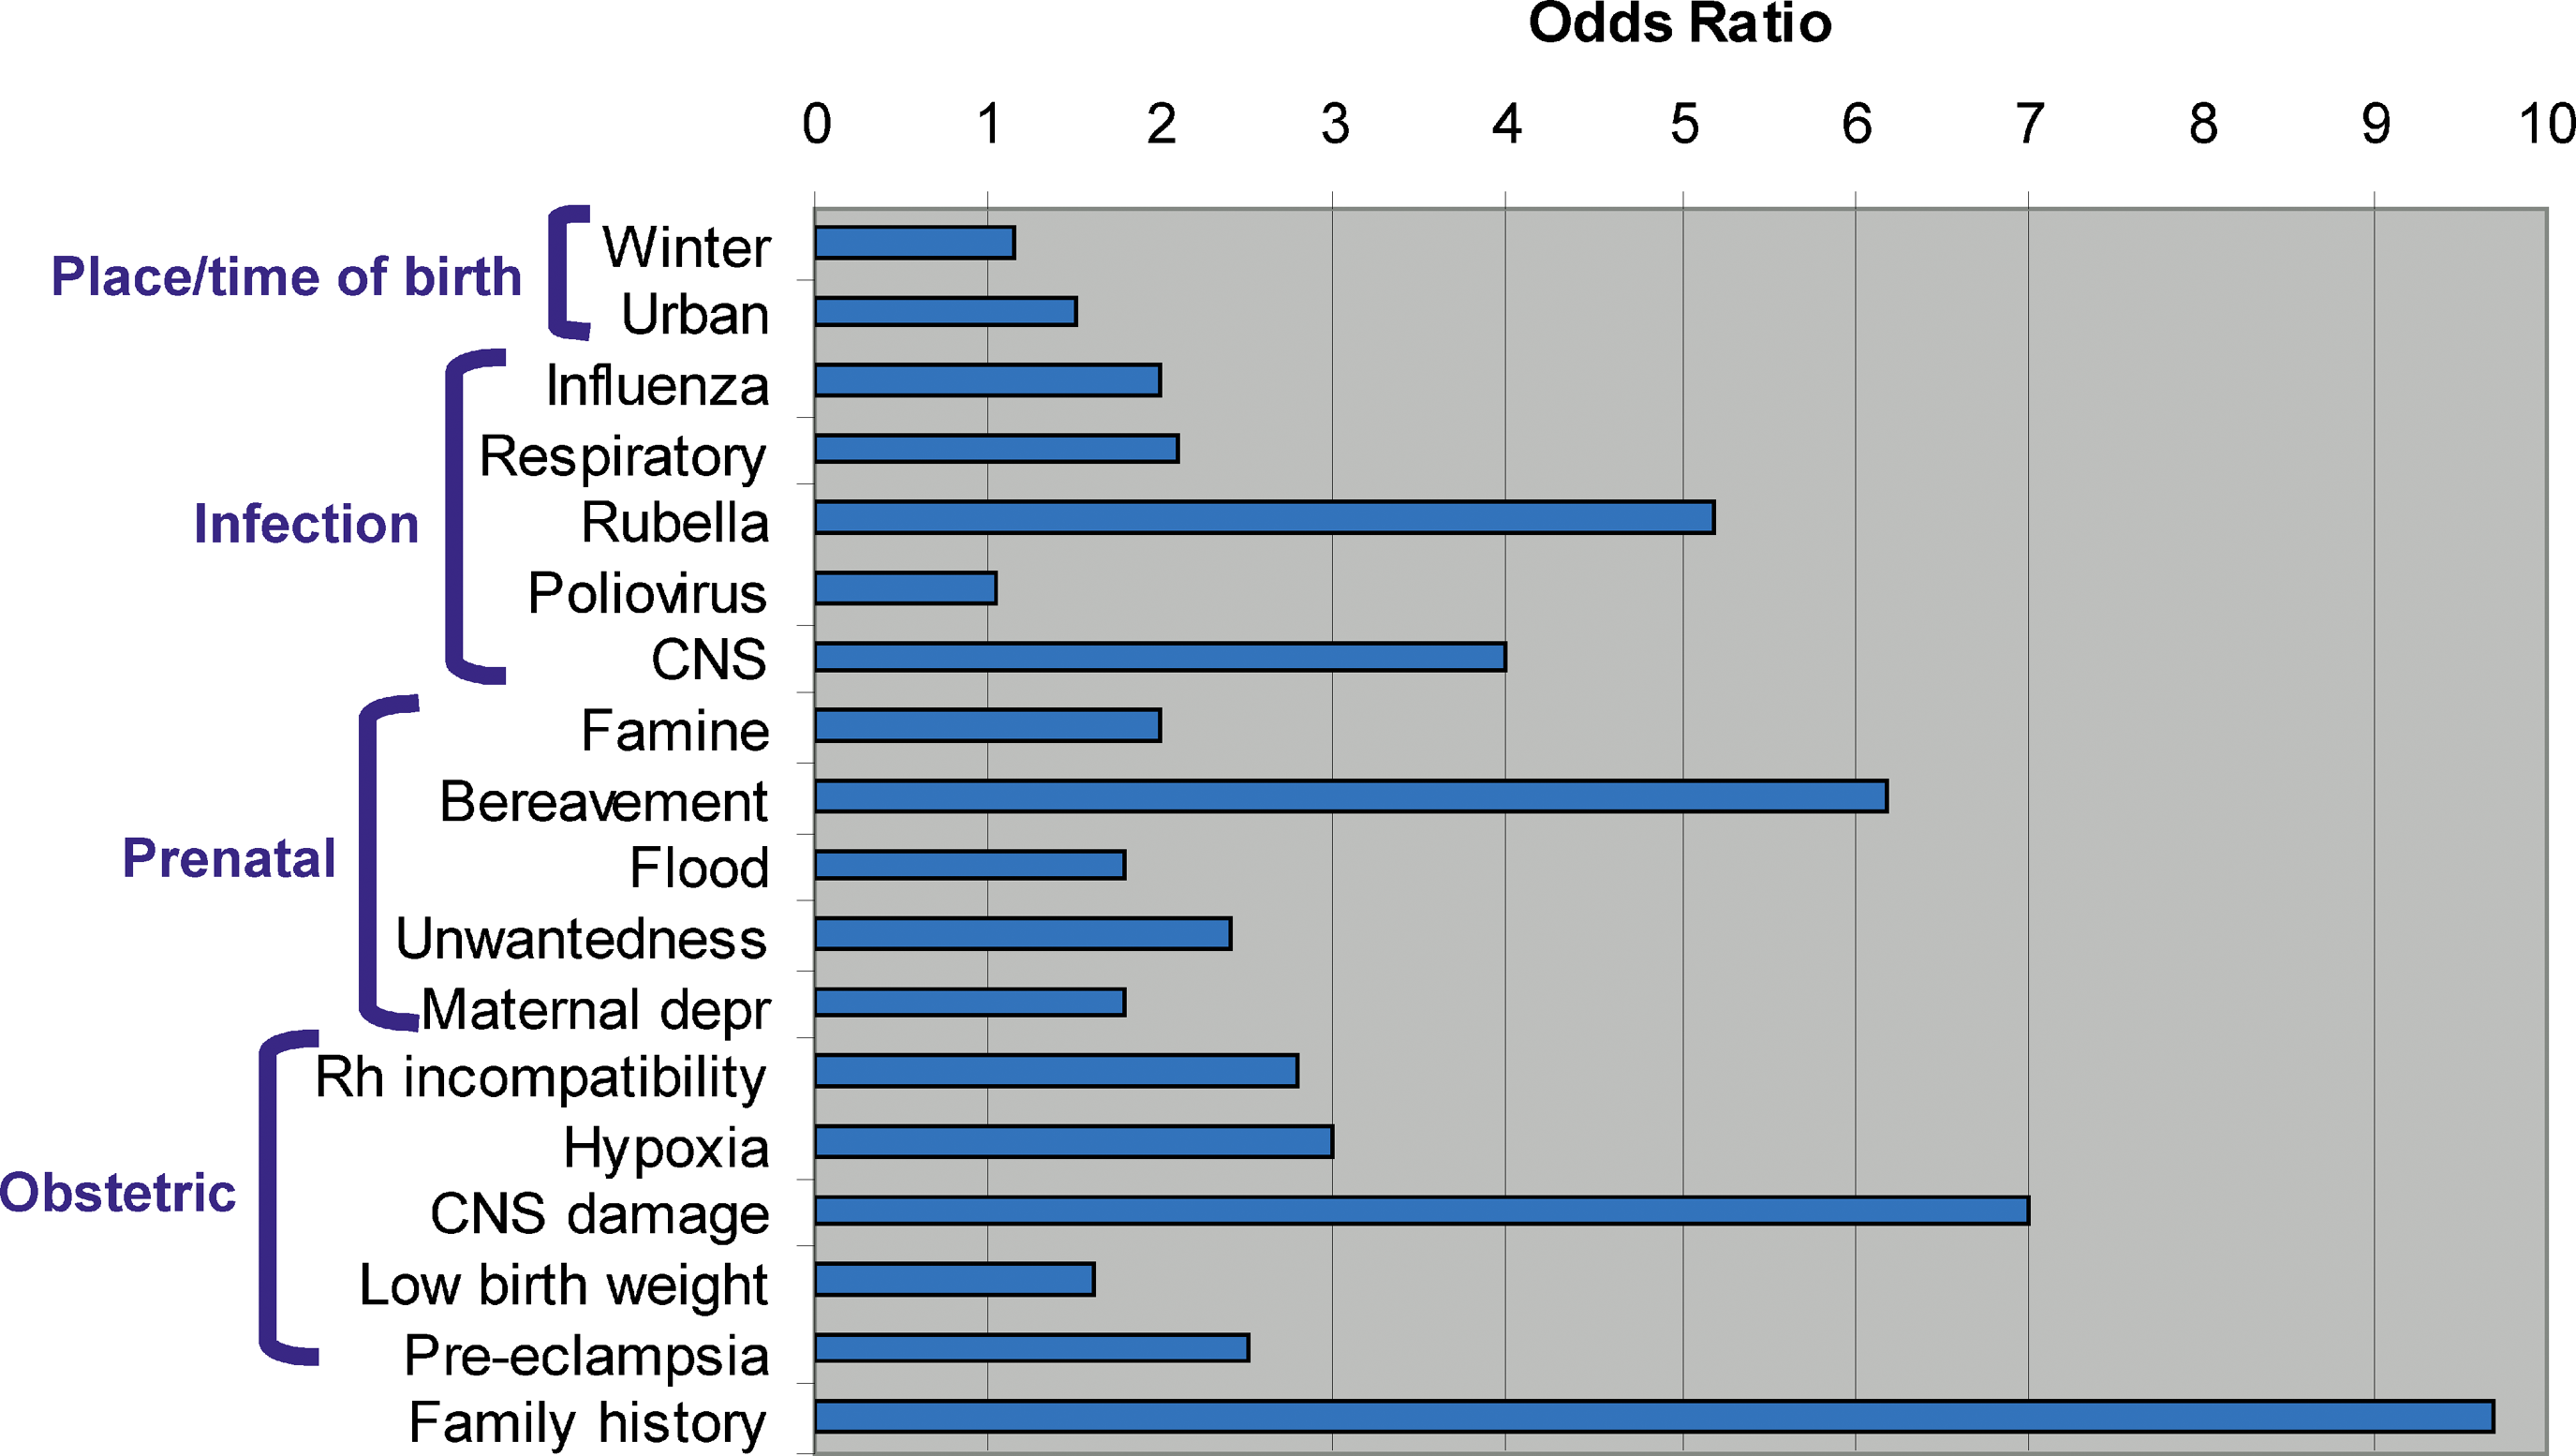
\includegraphics[width=\textwidth]{figure/risk_factors_of_schizophrenia.png}
	\caption[Risk factors of \scz]{Risk factors of \scz.
		Of all risk factors, family history of \scz\ was the largest, where risk of \scz\ can be more than 9 times higher than the general population for individual with a family history of \scz}
	\label{fig:riskfactors}
\end{figure}

Because evidence suggest there to be an interaction between prenatal infection and genetic variations \citep{Clarke2009}, it might be of particular interest to investigate the effect of prenatal infection to \scz.

Initial clues of involvements of prenatal infection in the etiology of \scz\ originates from the increased risk of \scz\ in individuals who were fetuses during the 1957 influenza epidemic \citep{Mednick1958}.
Moreover, it was observed that other than influenza, infection of HSV-2 and \textit{T.gondii} during gestation also increase the risk of \scz\citep{Brown2010}.
These evidences suggested prenatal infection might be associated with \scz.

Early studies of prenatal infection in \scz\ relied on ecological data to define the exposure status without any confirmation of maternal infection during pregnancy \citep{Brown2010}.
Therefore, the exposure status were inaccurate and unreliable, leading to inconsistent findings \citep{Brown2010}.  
Subsequently, birth cohorts, where infection was documented using different biomarkers during pregnancies, were conducted in order to obtain a better labeling of the exposure status \citep{Brown2010}.
From these cohorts, it was found that as long as an individual's mother was infected by any form of infectious agents (e.g. influenza, HSV-2 and \textit{T.gondii}) during gestation, an individual's risk of \scz\ increases \citep{Brown2010}.
This leads to the hypothesis that \gls{mia} \citep{Brown2010} rather than a particular infectious agent, is the main risk factor. 
\citet{Garbett2012a} suggested that one possible mechanism is that the maternal immune response to infection might have disrupted the brain development in the fetus, therefore predispose the fetus to \scz.

However, it is challenging to study the mechanism of \gls{mia}, because it is not possible to carry out controlled experiment on human samples due to ethical concerns.
Therefore rodent models is used as an alternative.
However, unlike physiological traits, psychiatric disorder such as \scz\ are characterized by symptoms related to higher level functioning such as hallucinations, delusion, disorganized speech etc. \citep{AmericanPsychiatricAssociation2013}, which are not readily detectable in rodents.
Therefore, as a compromise, rodent expressing ``\scz-like'' behaviours such as impaired prepulse inhibition, impaired working memory and reduced social interaction are considered as ``cases'' \citep{Meyer2007a}.

However, it is crucial to note that the behavioral abnormality is not unique to \scz, but can also be observed in autistic samples.
Moreover, \gls{mia} is also one of the risk factor for autism \citep{Brown2012}.
As a results, results from these rodent studies are non-specific to \scz\ or autism.
Discussion of the similarity and difference between autism and \scz\ is beyond the scope of the current thesis, therefore, the discussion is limited to \scz.

A common rodent model in the study of \gls{mia} is to use the viral analogue \gls{polyic} to induce the maternal immune response during pregnancy.
In this model, offspring exposed to \gls{polyic} displays phenotypes mirrors those observed in schizophrenia \citep{Li2009c,Meyer2009b,Li2010a}, such as deficiency in prepulse inhibition \citep{Cadenhead2000}.
Because \gls{polyic} only induce the \gls{mia} without infecting the fetuses, this model provide strong evidence that \gls{mia}, instead of the specific infection, contributes to the increased risk of \scz.	
	
\citet{Smith2007} were able to demonstrate that a single injection of \gls{il6} to the pregnant mouse can induce \scz-like behavior in the adult offspring. 
By eliminating the \gls{il6} from the maternal immune response, the behavior deficits associated with \gls{mia} were observed in the adult offspring \citep{Smith2007}.
This indicates that \gls{il6} is central to the process by which \gls{mia} causes long-term behavioral changes.

Recent studies of global gene expression patterns in \gls{mia}-exposed rodent fetal brains \citep{Oskvig2012,Garbett2012a} suggest that the post-pubertal onset of schizophrenic and other psychosis-related phenotypes might stem from attempts of the brain to counteract the environmental stress induced by \gls{mia} during its early development \citep{Garbett2012a}.
For example, genes with neuroprotective function such as crystallins also have additional roles in neuronal differentiation and axonal growth \citep{Garbett2012a}. 
By over-expressing these genes to counteract the environmental stress, the balance between neurogenesis and differentiation in the embryonic brain maybe disrupted. 
Based on these observations, \citet{Garbett2012a} propose that once the immune activation disappears, the normal brain development programme resumes with a time lag, result in permanent changes in connectivity and neurochemistry that might ultimately leads to \scz-like behaviours.

\begin{figure}
	\centering
	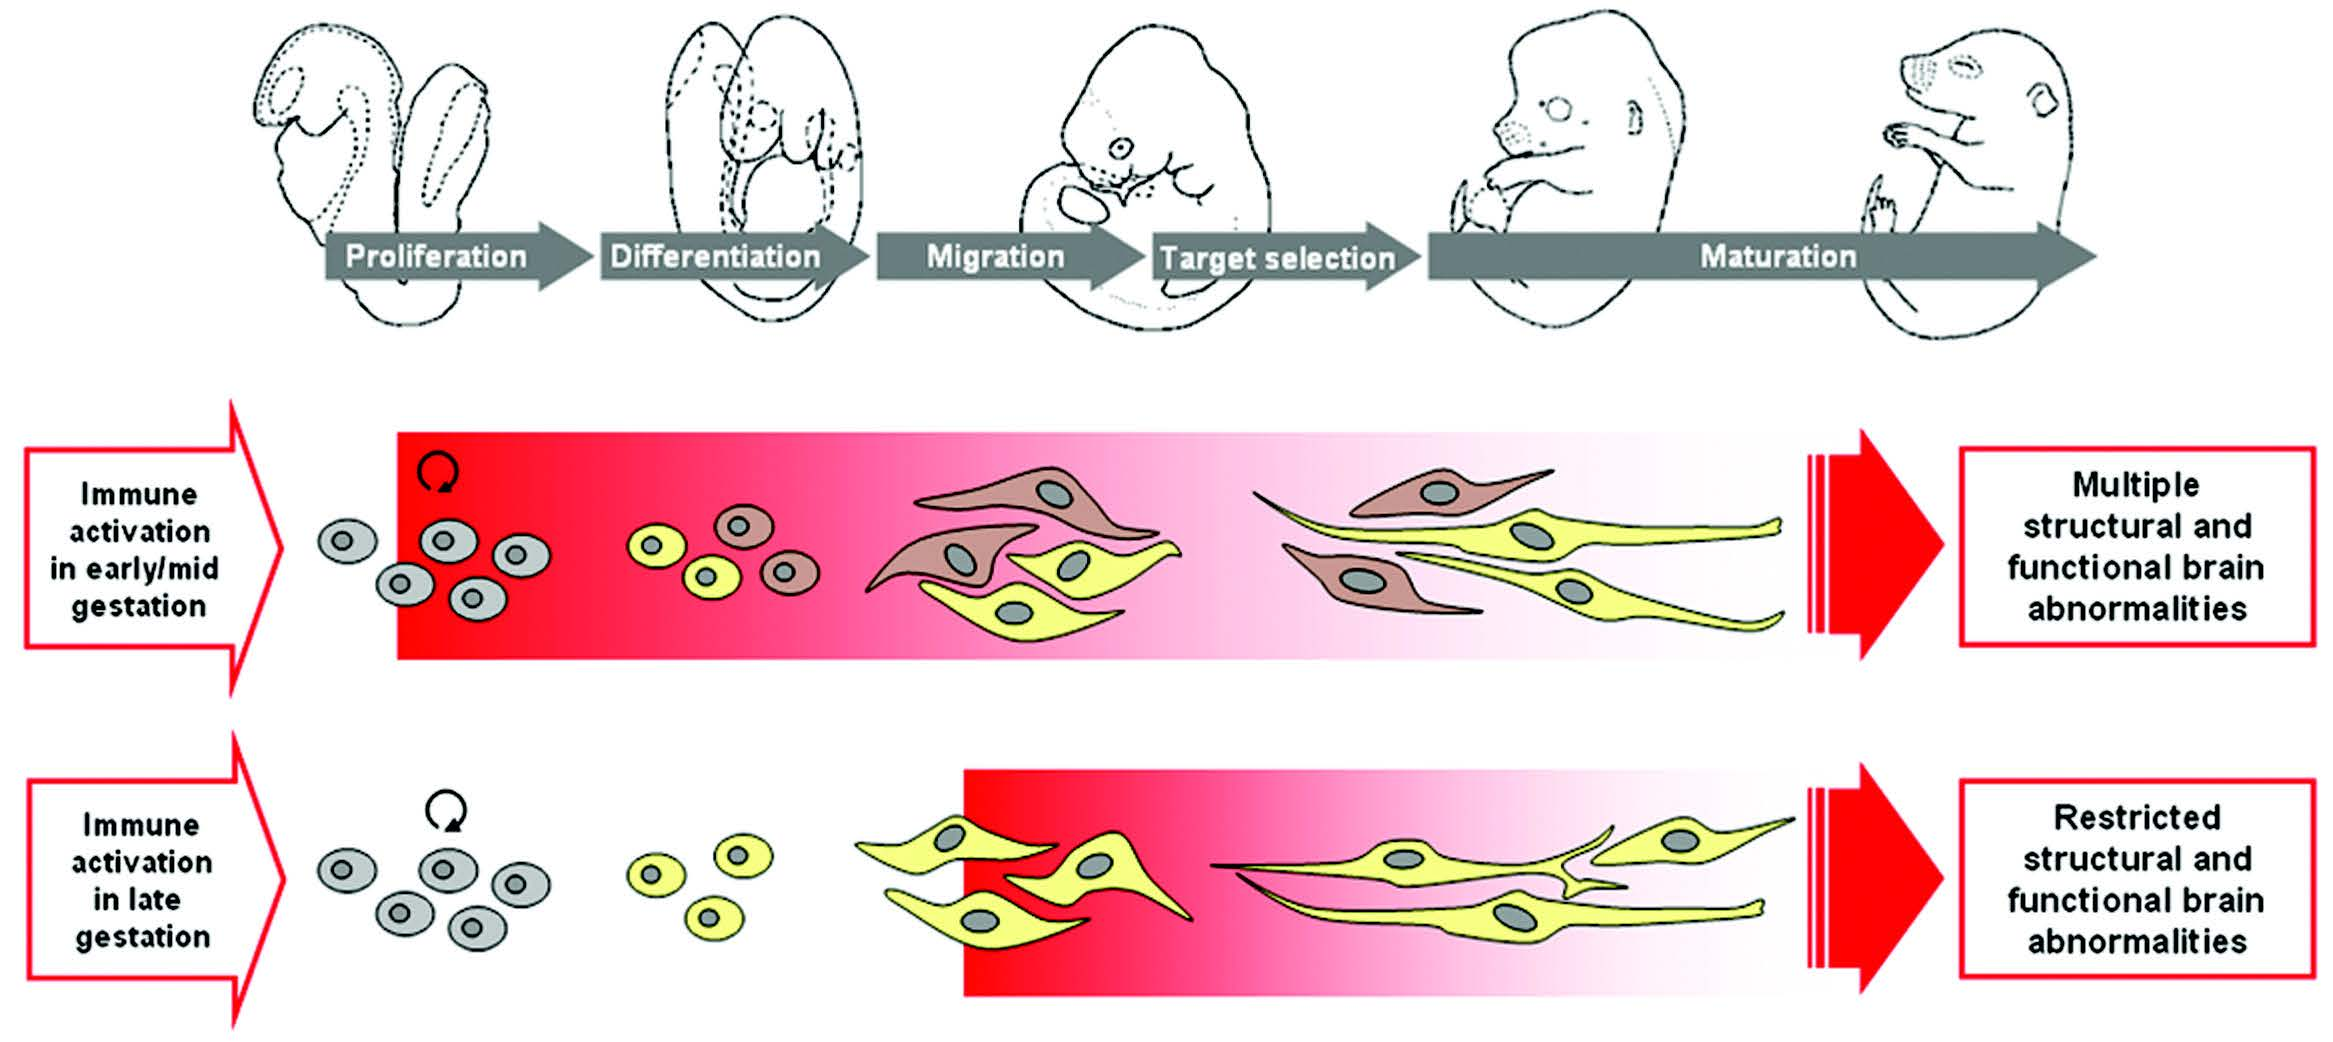
\includegraphics[width=\textwidth]{figure/mia_impact.jpg}
	\caption[Hypothesized model of the impact of prenatal immune challenge on fetal brain development]{Hypothesized model of the impact of prenatal immune challenge on fetal brain development.
		Maternal infection in early/mid pregnancy may affect early neurodevelopmental events in the fetal brain, thereby influencing the differentiation of neural precursor cells (grey) into particular neuronal phenotype (yellow or brown).
		This may predispose the developing fetal nervous system to additional failures leading to multiple structural and functional brain abnormalities in later life.
		Figure used with permission from Journal \citep{Meyer2007a}}
	\label{fig:miaEffect}
\end{figure}

On the other hand, an age dependent structural abnormalities in the mesoaccumbal and nigrostriatal dopamine systems were also found to be induced by \gls{mia} \citep{Vuillermot2010}.
Specifically, \gls{mia} induces an early abnormality in specific dopaminergic systems such as those in the striatum and midbrain region \citep{Vuillermot2010}.
Based on these observations, \citet{Meyer2007a} hypothesized that inflammation in the fetal brain during early gestation not only disrupts neuro-developmental processes such as cell proliferation and differentiation, it also predispose the developing nervous system to additional failures in subsequent cell migration, target selection, and synapse maturation (\cref{fig:miaEffect}) \citep{Meyer2007a}.
	
In a separate study by \citet{Giovanoli2013}, a lower dosage of \gls{polyic} were injected to the pregnant mice during early gestation.
The authors hypothesized that a low dose of \gls{polyic} will leads to restricted behavioral abnormalities in adulthood, thereby avoiding possible ceiling effects of the prenatal immunological manipulation on long-term brain and behavioral functions \citep{Giovanoli2013}. 
The offspring were then left undisturbed or exposed to unpredictable stress during peripubertal development.

An increased level of dopamine in the nucleus accumbens was observed in Offspring exposed to \gls{polyic} disregarding whether if they were exposed to postnatal stress.
Whereas serotonin (5-HT) were found to be decreased in the medial prefrontal cortex when exposed to postnatal stress regardless of prenatal exposure.
Only when the offspring were exposed to both \gls{polyic} and postnatal stress will they have an increased dopamine levels in the hippocampus or will sensorimotor gating and psychotomimetic drug sensitivity be affected \citep{Giovanoli2013}.
\citet{Giovanoli2013} therefore suggest that the prenatal insult serves as a ``disease primer'' that increase offspring's vulnerability to subsequent insults.

One of the critical consideration in the study of \gls{mia} is the specific gestation period of vulnerability to infection-mediated disturbance \citep{Meyer2007a}.
Early epidemiological studies have suggested that the second trimester of human pregnancy might be the vulnerability period.
However, in birth cohorts such as the Prenatal Determinants of \Scz, it was found that the time window with maximum risk for infection-mediated disturbance in brain development is earlier than the second trimester of human pregnancy, which can be as early as the first trimester \citep{Meyer2007a}.
By reviewing existing \gls{mia} studies, \citet{Meyer2007a} suggested the effect of \gls{mia} during late pregnancy is restricted to the late developmental programmes, thus have a more restricted pathological phenotype in the grown offspring compared to \gls{mia} during early pregnancy \citep{Meyer2007a}.
Subsequent \gls{mia} studies using the \gls{polyic} mouse model also support the hypothesis proposed by \citet{Meyer2007a}, where it was observed that \gls{mia} early in gestation event exert a more extensive impact on the phenotype of offspring \citep{Li2009c,Li2010a}.
	
Despite the more severe impact of \gls{mia} during early gestation, most \gls{mia} studies have been focusing on the mid-gestation period.
Therefore, there is a lack of understanding of the full molecular implication of early \gls{mia} events in adult brain.

The main goal of \scz\ research is to identify a effective treatment for \scz. 
One potential target is the n-3 \gls{pufa} \citep{Li2015,Trebble2003}.
In mouse, it was found that n-3 \gls{pufa} can inhibits the production of \gls{il6} \citep{Trebble2003} - a major mediator in \gls{mia} model \citep{Smith2007}.
Apart from its anti-inflammatory property, n-3 \gls{pufa} such as docosahexaenoic acid (DHA) also plays a critical role in the development of central nervous system \citep{Clandinin1999,Kitajka2002}.
Given its strong implication in neuronal functioning, it is possible that n-3 \gls{pufa} rich diet may reduce the symptoms of \scz, as reported by a recent study \citep{Li2015}.

Together, it is interesting for us to not only investigate the effect of \gls{mia} during early gestation, but also study the effect of different diet to the treatment of \scz.
As technology advances, global \gls{mrna} expression changes can now be examined using RNA Sequencing, therefore allowing us to investigate effect of early \gls{mia} exposure and n-3 \gls{pufa} rich diet to the expression pattern in the brain.

\subsection{RNA Sequencing}
Before the development of \gls{ngs} technology, the global gene expression changes can only be inspected by performing microarray analysis, which is based on probe hybridization.
With the development of \gls{ngs} technology, sequencing can be performed on the \gls{mrna} fragments.

Comparing to microarray, RNA Sequencing has a number of advantages, most notably, because RNA Sequencing does not rely on specific probe hybridization, it does not suffer from bias introduced by probe performances such as signal saturation, cross-hybridization, background noises and non-specific hybridization \citep{Zhao2014}.
Furthermore, alternative splicing analysis and de-novo transcript assembly can be readily performed on the same set of RNA Sequencing data.
On the other hand, de-novo assembly cannot be detected using microarray and specialized chips are required in order to perform alternative splicing analysis. 

However, the superior performance of RNA Sequencing does not come without a cost.
The first hurdle in the analysis of RNA Sequencing data is the sequence alignment.
As RNA sequencing generates sequence reads from the \gls{mrna} transcripts where the introns are usually spliced out, special consideration are required during alignment.
Specifically, one can either align the sequence reads directly to the transcriptome or to the reference genome.

The alignment to the transcriptome is relatively simple, the challenge however is that However, multiple isoform can share the same exon. 
Therefore there are a high level of mapping uncertainties, e.g. a single read can be aligned to multiple transcripts \citep{Li2011e}.
This results in difficulties when trying to quantify the expression level of individual transcripts. 

On the other hand, one can align the sequence reads directly to the reference genome. 
However, due to alternative splicing, splice aware algorithms such as  TopHat2 \citep{Kim2013}, STAR \citep{Dobin2013} and MapSplice \citep{Wang2010} must be used instead. 

Another difficulty is the differential expression analysis. 
In RNA Sequencing, the expression of a gene is represented by the number of reads aligned to the gene. 
However, unlike microarray, where the signal usually follows a normal distribution \citep{Hoyle2002,Giles2003}, the distribution of the RNA Sequencing count data are more complicated.

Early RNA Sequencing experiment assumes the gene expression counts to follows the Poisson distribution \citep{Marioni2008}, where the variance of the expression is expected to be equal to the mean of the expression.
However, it was found that the assumption of Poisson distribution is too restrictive, as an over-dispersion was typically observed in RNA Sequencing data \citep{Anders2010}.
Therefore, to overcome the problem of over-dispersion, differential expression analysis of RNA Sequencing data are required to model the expression using the negative binomial distribution \citep{Anders2010,Robinson2010} or the beta negative binomial distribution \citep{Trapnell2012}, instead of the Poisson distribution.
	\begin{figure}
		\centering
		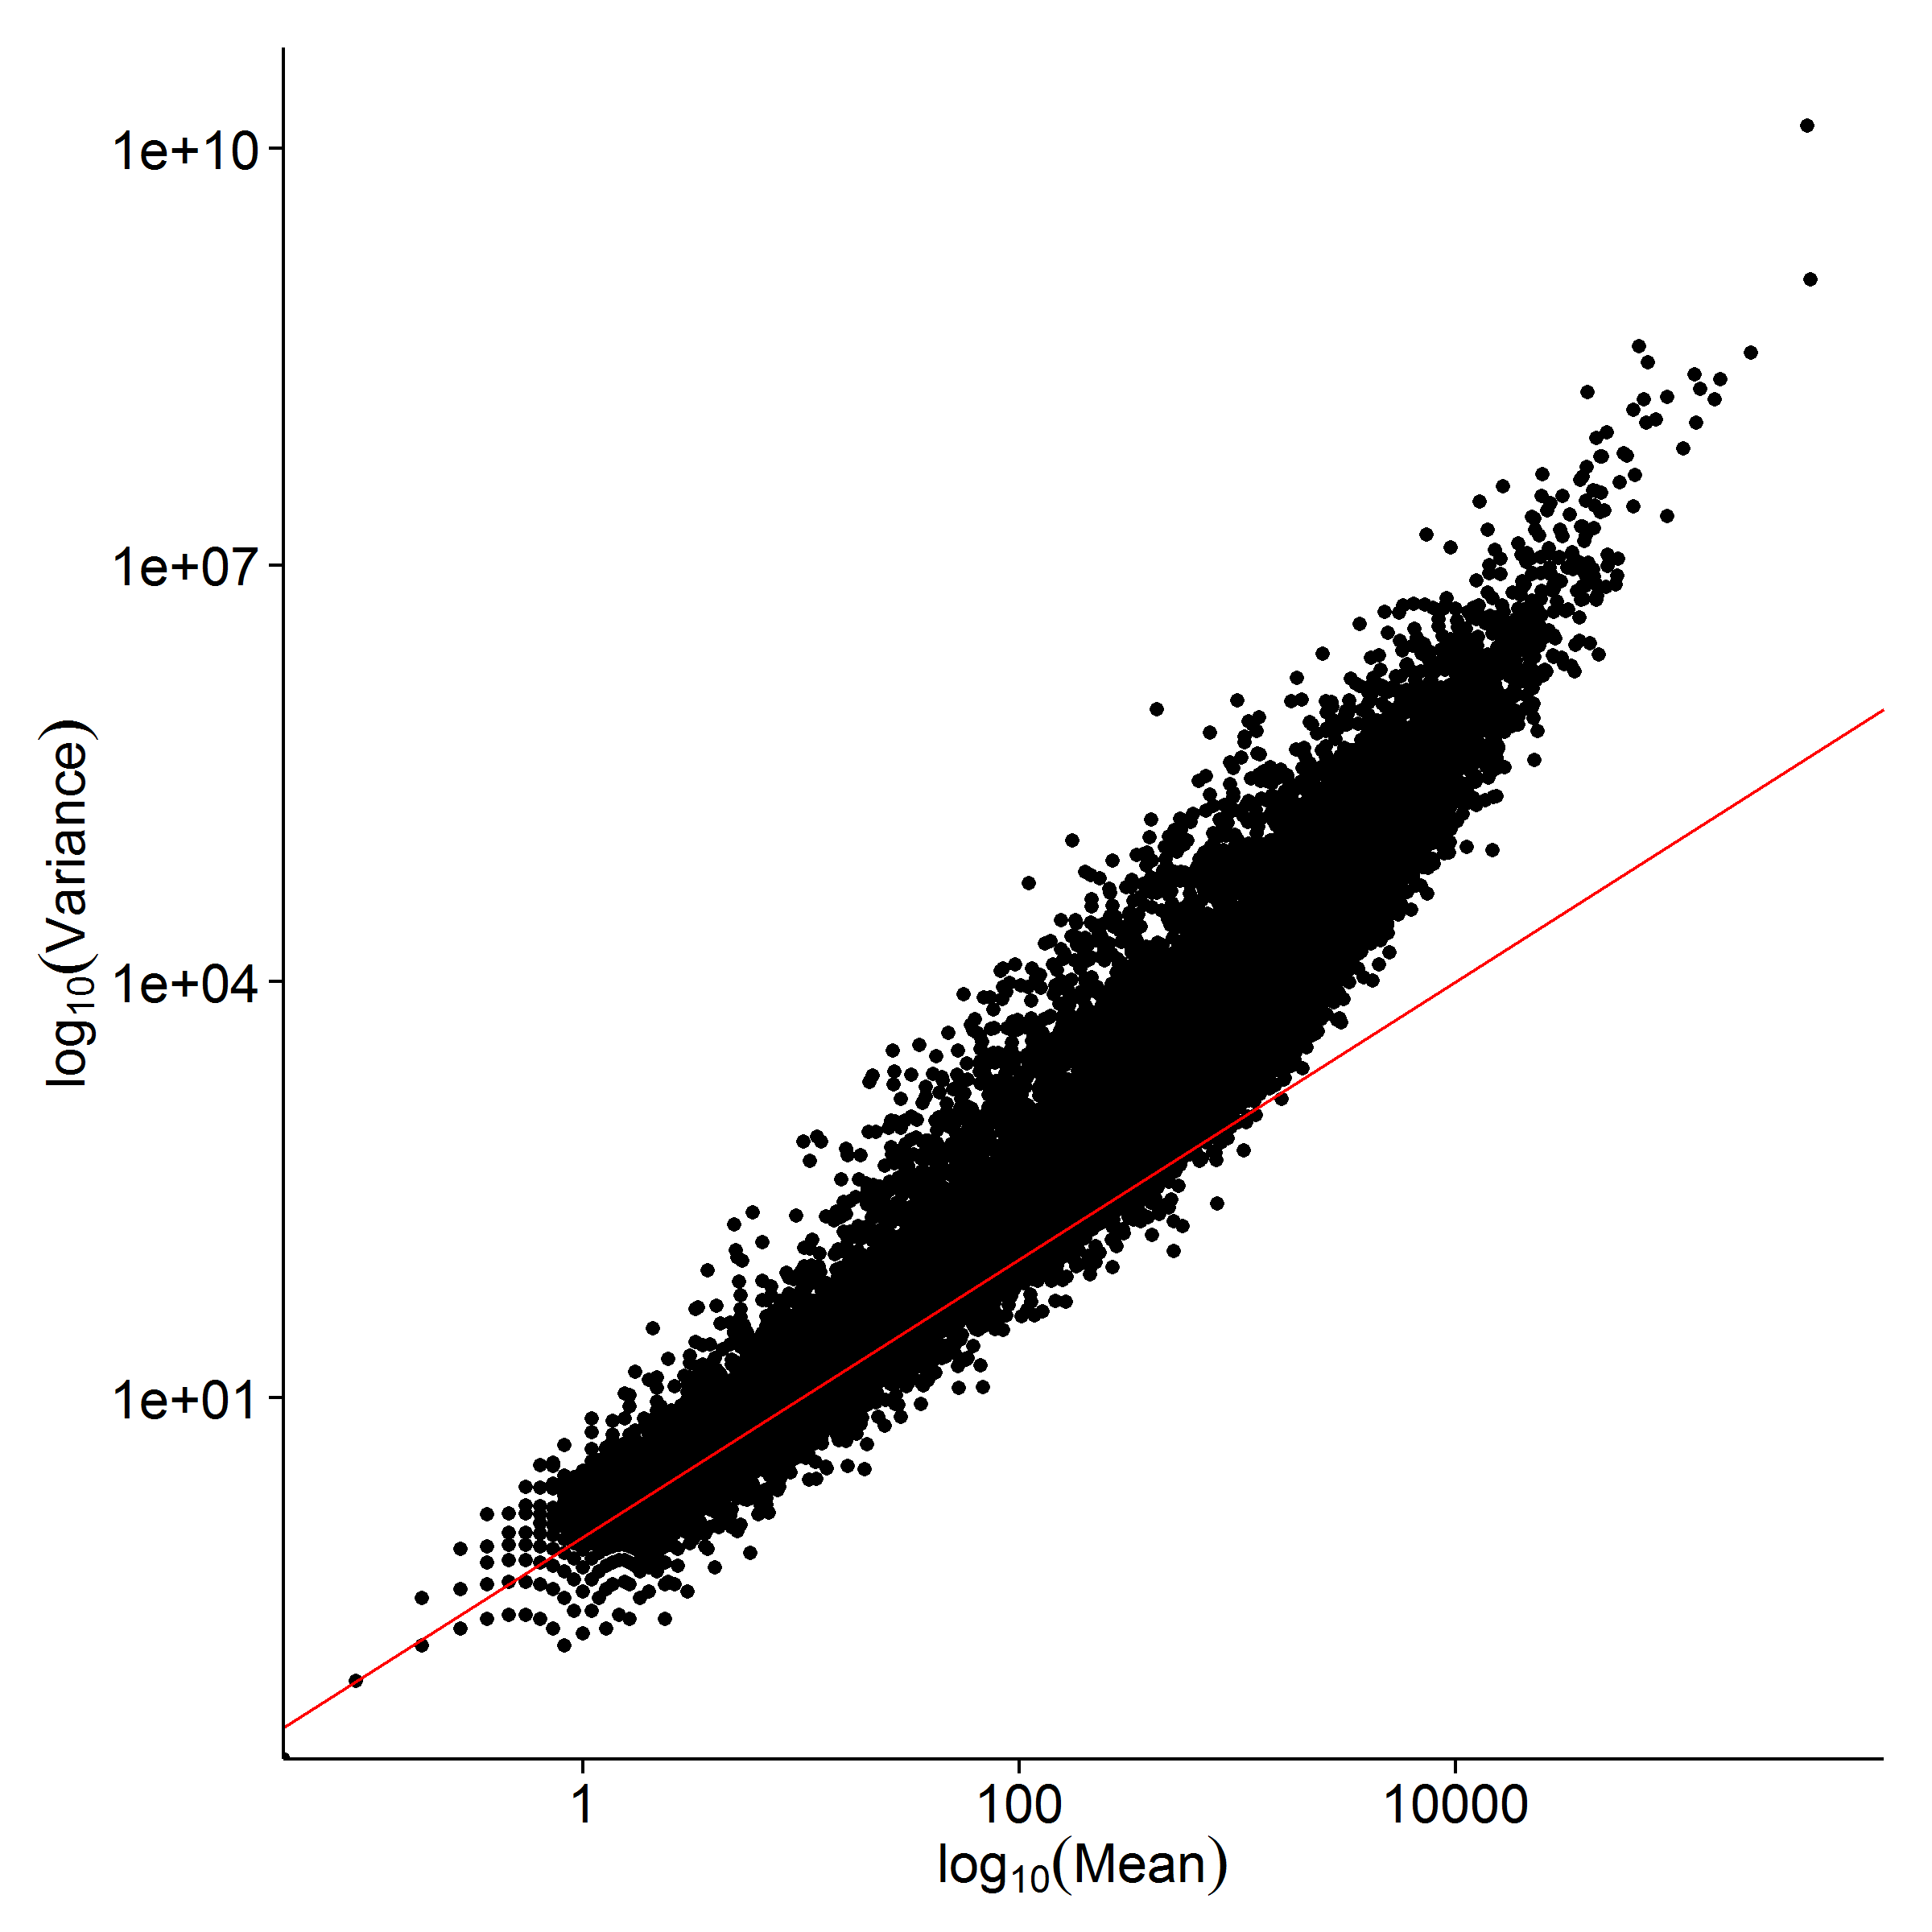
\includegraphics[width=0.5\textwidth]{figure/overdispersion.png}
		\caption[Over-dispersion observed in RNA Sequencing Count Data]{
			Over-dispersion observed in RNA Sequencing Count Data.
			If the RNA Sequencing count data follows the Poisson distribution, then the mean and variance of the data should be equal (follow the diagonal). 
			However, it was observed that as the mean increases, the variance increases even more, suggesting that there is an over-dispersion in the data. 
		}
	\end{figure}
	
By using the appropriate aligner for the alignment of the RNA sequencing data, and using the appropriate statistical modeling, RNA Sequencing can provide unprecedented power for the analysis of expression changes.
Therefore, RNA Sequencing might be an appropriate tool for the analysis of gene expression changes induced by \gls{mia} event and study the effect of the n-3 \gls{pufa} diet. 

\section{Summary}
The estimated \gls{SNP}-heritability for \scz\ by \citet{Bulik-Sullivan2015} suggest that the common variants might have accounted for most if not all of the heritability of \scz.
However, there are multiple concerns, firstly, \citet{Bulik-Sullivan2015} only considered a limited number of cases in the binary trait simulation. 
It is therefore unclear how the \gls{ldsc} perform in different binary traits.
Moreover, studies suggest that \gls{cnv} \citep{Szatkiewicz2014}, structural variations \citep{Walsh2008} and also rare mutations \citep{purcell2014polygenic} are contributing to the risk of \scz.
Also, considering the presence of gene-environment interactions can inflate the total heritability estimated for a disease \citet{zuk2012mystery}, it is likely for the \gls{SNP}-heritability estimated by \citet{Bulik-Sullivan2015} to be too high.
It might therefore be interesting to see if an alternative method can result in the same estimates  as provided by \gls{ldsc}.

In this thesis, we would first like to perform an extensive simulation to investigate the performance of \gls{ldsc} given different genetic architectures, sampling strategies and types of traits. 
We are especially interested in the performance of \gls{ldsc} for binary traits. 
In addition, we would like to develop an independent algorithm to estimate the \gls{SNP}-heritability of \scz.
This will allow us to assess whether if the \gls{SNP}-heritability estimated by \gls{ldsc} is correct.

On the other hand, with the presence of the gene-environment interaction \citep{Tienari2004,Clarke2009}, the total heritability of \scz\ might be overestimated \citet{zuk2012mystery}.
Therefore, the proportion of environmental influence to \scz\ might be higher than expected.
One of the environmental factor interacting with genetic factors is the prenatal infection \citet{Clarke2009}.
Given its importance in the etiology of \scz, it is of our interest to study the impact of prenatal infection to the transcriptome pattern of the brain.
Hence, we perform a RNA Sequencing study to capture gene expression changes induced by early (\gls{gd}9) \gls{mia} events in the mouse cerebellum using the \gls{polyic} mouse model.
Additionally, because our lab has recently found that n-3 \gls{pufa} rich diet might help to reduce \scz-like behaviour in mice exposed to early \gls{mia} insults \citep{Li2015},we are also interested in investigating the effect of n-3 \gls{pufa} rich diet in the gene expression pattern in the brain of the \gls{mia} samples. 

In summary, this thesis is divided into three parts. 
We first investigate the performance of \gls{ldsc} in \Cref{heritabilityChapter} and introduce \gls{shrek}, an alternative algorithm to \gls{ldsc} for the estimation of \gls{SNP}-heritability using \gls{GWAS} summary statistics. 
This should allow us to assess whether if the \gls{SNP}-heritability of \scz\ estimated by \gls{ldsc} is correct.

In the next chapter, we introduce the RNA Sequencing study on the effect of early \gls{mia} insult and n-3 \gls{pufa} rich diet on gene expression of the mouse cerebellum.
This should provide understanding to the impact of \gls{mia} in early gestation and also provide insight into possible treatment target for \scz\ induced by \gls{mia}.

Lastly, we will summarize and conclude all findings in \Cref{conclusionChapter} where future perspectives on genetic studies of \scz\ will be provided.

\chapter{Heritability Estimation}
\label{heritabilityChapter}
\section{Introduction}
\glsreset{shrek}
\citet{Bulik-Sullivan2015} estimated the \gls{SNP}-heritability of \scz\ to be around 55.5\%, which suggest the common variants have accounted for majority of the heritability of \scz.
However, studies have found that \gls{cnv} \citep{Szatkiewicz2014}, structural variations \citep{Walsh2008} and also rare mutations \citep{purcell2014polygenic} can also contribute to the risk of \scz.
Additionally, with the presence of gene-environment interaction, the total heritability estimated for \scz\ might be inflated \citet{zuk2012mystery}. 
It is therefore likely that \citet{Bulik-Sullivan2015} has overestimated the \gls{SNP}-heritability of \scz.

It is noted that \citet{Bulik-Sullivan2015} only conducted a limited number of simulation on binary trait data, therefore it is unclear how \gls{ldsc} performs in other condition.
Additionally, because \citet{Bulik-Sullivan2015} found that \gls{ldsc} has a larger standard error for oligogenic traits, it might be beneficial for us to develop an alternative algorithms that has robust performance for all traits. 

Herein, we introduce \gls{shrek}, an alternative algorithm to \gls{ldsc} for the estimation of \gls{SNP}-heritability using \gls{GWAS} summary statistics.
We also investigate the performance of \gls{shrek} and \gls{ldsc} on different traits by performing a comprehensive simulation, using \gls{gcta} as a golden standard. 
Finally, we estimate the \gls{SNP}-heritability of \scz\ using \gls{shrek} and \gls{ldsc} to investigate whether the \gls{SNP}-heritability estimated by \citet{Bulik-Sullivan2015} is correct.

The work in this chapter were done in collaboration with my colleagues who have kindly provided their support and knowledges to make this piece of work possible.
Dr Johnny Kwan, Dr Miaxin Li and Professor Sham have helped to lay the foundation of this study. 
Dr Timothy Mak has derived the mathematical proof for our heritability estimation method. 
Miss Yiming Li, Dr Johnny Kwan, Dr Miaxin Li, Dr Desmond Campbell, Dr Timothy Mak and Professor Sham have helped with the derivation of the standard error of the heritability estimation. 
Dr Henry Leung has provided critical suggestions on the implementation of the algorithm.

\section{Methodology}			
\subsection{Basic Concept of SHREK}
The fundamental idea of \gls{shrek} is that the summary statistics of a \gls{SNP} from a \gls{GWAS} should represent the among of phenotypic variance it explain.
By definition, the coefficient of determination ($r^2$) is the variance in the dependent variable that is predictable by the independent variable.
If we define the phenotype as the dependent variable and the genotype as the independent variable, the coefficient of determination between the phenotype and genotype equals to the heritability explained by the specific \gls{SNP}.

Therefore, if we assume the summary statistic of \gls{SNP} $i$ be $t_i$, which follow the student-t distribution under the null, the coefficient of determination between \gls{SNP} $i$ and the phenotype can be represented as 
\begin{equation}
r_i^2=\frac{t_i^2}{n-2+t_i^2}
\label{eq:coefficientDetermination}
\end{equation}
where $n$ is the number of samples.
When $n$ is large, $t_i^2$ will converge to $\chi^2$ distribution under the null, with mean equal to 1.
Therefore, we can express \cref{eq:coefficientDetermination} as
\begin{equation}
\hat{r_i}^2=\frac{t_i^2-1}{n-2+t_i^2}
\label{eq:cDShrek}
\end{equation}
If all \glspl{SNP} are independent of each other, the \gls{SNP}-heritability will simply be
\begin{equation}
\text{SNP-heritability}=\sum_i\hat{r_i}^2
\end{equation}

However, in reality \glspl{SNP} are correlated with each other and will inflate the summary statistic. 
Therefore, we must take into account of \gls{LD} when we estimate the \gls{SNP}-heritability.

\subsection{Derivation of SHREK}
\label{sec:derive}
Here, we provide a step by step derivation of \gls{shrek} showing how can the \gls{LD} be incorporate into the calculation of \gls{SNP}-heritability using only the summary statistic.
First, we assume the phenotype $\boldsymbol{y}$ and genotype matrix  $\boldsymbol{X}$ are standardized such that
\begin{align*}
\boldsymbol{y}\sim f(0,1) \\
\boldsymbol{X}\sim f(0,\boldsymbol{R})
\end{align*}
Where $f(m, \boldsymbol{V})$ denotes a general distribution with mean $m$ and variance $\boldsymbol{V}$ with $\boldsymbol{R}$ as the \gls{LD} matrix.

The linear regression between $\boldsymbol{X}$ and $\boldsymbol{y}$ can then be defined as
\begin{align}
\boldsymbol{y}=\boldsymbol{X}\boldsymbol{\beta}+\boldsymbol{\epsilon}
\label{eq:matrixRegress}
\end{align}
where $\boldsymbol{\epsilon}$ is the error term, account for the non-genetic elements contributing to the phenotype.

As heritability is defined as $\frac{V_G}{V_P}$ where $V_G$ is the variance of the genetic factor and $V_P$ is the variance of the phenotype, we can obtain
\begin{align}
\text{Heritability}&=\frac{\mathrm{Var}(\boldsymbol{X}\boldsymbol{\beta})}{\mathrm{Var}(\boldsymbol{y})}\\
&=\mathrm{Var}(\boldsymbol{X}\boldsymbol{\beta})
\end{align}
We then assume $\boldsymbol{\beta} = (\beta_1, \beta_2,\dots,\beta_m)^t$ follows the distribution:
\begin{align*}
\boldsymbol{\beta}&\sim f(0,\boldmath{H})\\
\boldsymbol{H}&=diag(\boldsymbol{h^2})\\
\boldsymbol{h^2}&=(h_1^2,h_2^2,\dots,h_m^2)^t
\end{align*}
where $\boldsymbol{h^2}$ is the variance of the ``true'' effect. 
$\mathrm{Var}(\boldsymbol{X}\boldsymbol{\beta})$ can then be expressed as
\begin{align}
\mathrm{Var}(\boldsymbol{\beta}\boldsymbol{X}) &= \mathrm{E}_X\mathrm{Var}_{\beta|X}(\boldsymbol{X}\boldsymbol{\beta})+\mathrm{Var}_X\mathrm{E}_{(\beta|X)}(\boldsymbol{X}\boldsymbol{\beta}) \nonumber\\
&=\mathrm{E}_X(\boldsymbol{X}^t\mathrm{Var}(\boldsymbol{\beta})\boldsymbol{X}) \nonumber\\ 
&= \mathrm{E}_X(\boldsymbol{X}^t\boldsymbol{HX}) \nonumber\\
&=\mathrm{Tr}(\mathrm{Var}(\boldsymbol{X}\boldsymbol{H})) \nonumber\\
&=\sum_ih_i^2
\label{eq:proveHerit}
\end{align}
Therefore
\begin{equation}
\text{SNP-heritability}=\sum_ih_i^2
\label{eq:sumH}
\end{equation}

Now the covariance between \gls{SNP}$_i$ ($\boldsymbol{x_i}$) and $\boldsymbol{y}$ can be expressed as 
\begin{align}
\mathrm{Cov}(\boldsymbol{x_i}, \boldsymbol{y})&=\mathrm{Cov}(\boldsymbol{x_i},\boldsymbol{X\beta}+\boldsymbol{\epsilon})\notag\\
&=\mathrm{Cov}(\boldsymbol{x_i},\boldsymbol{X\beta})\notag\\
&=\mathrm{Cov}(\boldsymbol{x_i},\boldsymbol{X})\boldsymbol{\beta}\notag\\
&=\boldsymbol{R_i\beta}
\end{align}

As both $\boldsymbol{X}$ and $\boldsymbol{y}$ are standardized, their covariance is equal to their correlation
$$
\mathrm{Cov}(\boldsymbol{x_i},\boldsymbol{y})=\mathrm{Cor}(\boldsymbol{x_i},\boldsymbol{y})=\rho_i
$$

In reality, the \emph{observed} correlation is usually error-prone. 
Therefore the observed correlation between SNP$_i$ and the phenotype is defined as 
$$
\hat{\rho_i} = \rho_i+\frac{\epsilon_i}{\sqrt{n}}
$$
for some error $\epsilon_i$. 
The distribution of the correlation coefficient about the true correlation $\rho_i$ is approximately
$$
\hat{\rho_i}\sim f\left(\rho_i, \frac{(1-\rho_i^2)^2}{n}\right)
$$

By making the assumption that $\rho_i$ is close to 0 for all $i$, we get
\begin{align}
\mathrm{E}(\epsilon_i|\rho_i)&\sim 0\\
\mathrm{Var}(\epsilon_i|\rho_i)&\sim 1
\label{eq:assump}
\end{align}
If we define the $z$-statistic and $\chi^2$-statistic as
\begin{align}
z_i&=\hat{\rho_i}\sqrt{n}\\
\chi_i^2&=z_i^2\nonumber\\
&=\hat{\rho_i^2}n
\end{align}
We can express $\chi^2$ as 
\begin{align}
\chi_i^2&=\hat{\rho_i^2}n\nonumber\\
&=n\left(\boldsymbol{R_{i}\beta}+\frac{\epsilon_i}{\sqrt{n}}\right)^2
\end{align}
and
\begin{align}
\mathrm{E}(\chi_i^2)&\approx n\boldsymbol{R_i}^t\boldsymbol{H}\boldsymbol{R_i}+1\nonumber\\
&=n\sum_jR_{ij}^2h_j^2+1\\
\end{align}
To derive least square estimates of $\boldsymbol{h^2}$, we need to find $\hat{\boldsymbol{h}^2}$ which minimizes
\begin{align}
&\sum_i\left(\chi_i^2-\mathrm{E}\left(\chi_i^2\right)\right)^2\nonumber\\
=&\sum_i\left(\chi_i^2-\left(n\sum_jR_{ij}^2\hat{h^2_j}+1\right)\right)^2
\label{eq:lseChi}
\end{align}
By defining 
\begin{equation}
f_i=\frac{\chi_i^2-1}{n}
\label{eq:defineF}
\end{equation}
\cref{eq:lseChi} becomes
\begin{align}
\sum_i\left(\chi_i^2-\mathrm{E}\left(\chi_i^2\right)^2\right)&=\sum_i\left(f_i-\sum_jR_{ij}^2h_j^2\right)^2\\
&=\boldsymbol{f^tf-2f^tR_{sq}\hat{h^2}+\hat{h^2}R^t_{sq}R_{sq}\hat{h^2}}
\end{align}
where $\boldsymbol{R_{sq}=R\circ R}$ and $\circ$ denotes the element-wise product (Hadamard product). By differentiating with respect to $\hat{h^2}$ and set to 0,we get
\begin{align}
2\boldsymbol{R_{sq}^t}\boldsymbol{R_{sq}}\boldsymbol{\hat{h^2}}-2\boldsymbol{R_{sq}f}&=0\nonumber\\
\boldsymbol{R_{sq}\hat{h^2}}&=\boldsymbol{f}
\label{eq:shrekEq}
\end{align}

Remember from \cref{eq:sumH} that \gls{SNP}-heritability can be represent as $\sum_ih_i^2$, therefore we can express the estimated \gls{SNP} heritability as 
\begin{align}
\boldsymbol{R_{sq}\hat{h^2}}&=\boldsymbol{f}\nonumber\\
\boldsymbol{\hat{h^2}}&=\boldsymbol{R_{sq}}^{-1}\boldsymbol{f}\nonumber\\
\text{SNP-heritabilility}&=\boldsymbol{1}^t\boldsymbol{R_{sq}}^{-1}\boldsymbol{f}
\label{eq:finalShrek}
\end{align}

\subsection{Calculation Standard Error}
It is also essential to estimate the standard error of the estimate.
Based on \cref{eq:finalShrek}, the variance of the \gls{SNP}-heritability can be defined as
\begin{equation}
\mathrm{Var}(\hat{\text{SNP-heritability}})=\boldsymbol{1}^t\boldsymbol{R_{sq}}^{-1}\mathrm{Var}(\boldsymbol{f})\boldsymbol{R_{sq}}^{-1}\boldsymbol{1}
\label{eq:varHvarf}
\end{equation}
Based on \cref{eq:varHvarf}, it is observed that in order to calculate the variance of the estimate, $\mathrm{Var}(\boldsymbol{f})$ is required.

We first consider genotype $x_i$ has a standard normal mean $z_i$ and non-centrality parameter $\mu_i$ such that
\begin{align}
\mathrm{E}[x_i]&=\mathrm{E}[z_i+\mu_i] \nonumber\\
&=\mu_i\\
\mathrm{Var}(x_i)&=\mathrm{E}[x_i^2]-\mathrm{E}[x_i]^2\nonumber\\
&=\mathrm{E}[z_i^2+\mu_i^2+2z_i\mu_i]-\mu_i^2\nonumber\\
&=\mathrm{E}[z_i^2]+\mathrm{E}[\mu_i^2]-\mu_i^2\nonumber\\
&=1\\
\mathrm{Cov}(x_i,x_j)&=\mathrm{E}[x_ix_j]-\mathrm{E}[x_i]\mathrm{E}[x_j]\nonumber\\
&=\mathrm{E}[(z_i+\mu_i)(z_j+\mu_j)]-\mu_i\mu_j\nonumber\\
&=\mathrm{E}[z_iz_j]
\end{align}
Because the genotypes are standardized, $\mathrm{Cov}(x_i,x_j)=\mathrm{Cor}(x_i,x_j)=R_{ij}$, with $R_{ij}$ being the \gls{LD} between \gls{SNP}$_i$ and \gls{SNP}$_j$.
$\mathrm{Cov}(\chi_i^2, \chi_j^2)$ can then be calculated as 
\begin{align}
\mathrm{Cov}(\chi_i^2, \chi_j^2)&=\mathrm{Cov}\left((z_i+\mu_i)^2,(z_j+\mu_j)^2\right)\nonumber\\
&=\mathrm{Cov}\left(z_i^2+\mu_i^2+2z_i\mu_i, z_j^2+\mu_j^2+2z_j\mu_j \right)\nonumber\\
&=\mathrm{Cov}(z_i^2,z_j^2)+4\mu_i\mu_j\mathrm{Cov}(z_i,z_j)\nonumber\\
&=\mathrm{E}(z_i^2z_j^2)-\mathrm{E}(z_i^2)\mathrm{E}(z_j^2)+4\mu_i\mu_j\mathrm{E}(z_iz_j)-\mathrm{E}(z_i)\mathrm{E}(z_j)\nonumber\\
&=\mathrm{E}(z_i^2z_j^2)+4\mu_i\mu_j\mathrm{E}(z_iz_j)-1
\end{align}

As 
$$
z_i|z_j\sim N(\mu_i+R_{ij}(z_j-\mu_j),1-R_{ij}^2)
$$
and $\mathrm{E}[z_iz_j]=R_{ij}$, $\mathrm{E}[z_i^2z_j^2]$ can be expressed as
\begin{align*}
\mathrm{E}[z_i^2z_j^2]&=\mathrm{Var}[z_iz_j]+\mathrm{E}[z_iz_j]^2\\
&=\mathrm{E}[\mathrm{Var}(z_iz_j|z_i)]+\mathrm{Var}[\mathrm{E}[z_iz_j|z_i]]+R_{ij}^2\\
&=\mathrm{E}[z_j^2\mathrm{Var}(z_i|z_j)]+\mathrm{Var}[z_j\mathrm{E}[z_i|z_j]]+R_{ij}^2\\
&=(1-R_{ij}^2)\mathrm{E}[z_j^2]+\mathrm{Var}(z_j(\mu_i+R_{ij}(z_j-\mu_j)))+R_{ij}^2\\
&=(1-R_{ij}^2)+\mathrm{Var}(z_j\mu_i+R_{ij}z_j^2-\mu_jz_jR_{ij})+R_{ij}^2\\
&=1+\mu_i^2\mathrm{Var}(z_j)+R_{ij}^2\mathrm{Var}(z_j^2)-\mu_j^2R_{ij}^2\mathrm{Var}(z_j)\\
&=1+2R_{ij}^2
\end{align*}
As a result, $\mathrm{Cov}(\chi_i^2, \chi_j^2)$ becomes
\begin{equation}
\mathrm{Cov}(\chi_i^2,\chi_j^2) = 2R_{ij}^2+4R_{ij}\mu_i\mu_j
\label{eq:finalChi}
\end{equation}
But then, 
\begin{align}
\mathrm{E}(z_iz_j) &= R_{ij}+\mu_i\mu_j \nonumber \\
\mathrm{E}(z_iz_j-R_{ij})&=\mu_i\mu_j
\end{align}
Therefore
\begin{align}
\mathrm{Cov}(\chi_i^2, \chi_j^2)=4R_{ij}z_iz_j-2R_{ij}^2
\label{eq:varF}
\end{align}
Additionally, it was observed that
\begin{align}
\mathrm{E}[\hat{z_i}\hat{z_j}]&=\mathrm{E}[(z_i+\mu_i)(z_j+\mu_j)]\notag\\
&=\mu_i\mu_j+\mathrm{E}[z_iz_j]\nonumber\\
&=\mu_i\mu_j+R_{ij}
\label{eq:zzuu}
\end{align}
where $\hat{z_i}$ is the \emph{observed} $z$-statistic ($\boldsymbol{\hat{z}} = \sqrt{\boldsymbol{\chi^2}}$ from \cref{eq:defineF}, with the direction of effect as its sign).
Substituting \cref{eq:zzuu} and \cref{eq:varF} into \cref{eq:varHvarf} in matrix form, the variance of the estimate can be expressed as
\begin{align}
\mathrm{Var}(\hat{\text{SNP-heritability}}) &=\boldsymbol{1}^t\boldsymbol{R_{sq}}^{-1}\frac{2\boldsymbol{R_{sq}}+4\boldsymbol{R}\circ \boldsymbol{\hat{z}\hat{z}}^t}{n^2}\boldsymbol{R_{sq}}^{-1}\boldsymbol{1}
\label{eq:covH}
\end{align}

Given the direction of effect, \cref{eq:covH} should in theory provide the correct estimate of the standard error.
However, the direction of effect are not always available and in such scenario, \cref{eq:covH} cannot provide an accurate estimation of the standard error.
As $n\times \boldsymbol{f}+1$ is approximately $\chi^2$ distributed, we might view \cref{eq:shrekEq} as a decomposition of a vector of $\chi^2$ distributions with degree of freedom of 1. 
Replacing the vector $\boldsymbol{f}$ with a vector of 1, the ``effective number''($e$) of association \citep{Li2011} can be calculated. 
Substituting $e$ into the variance equation of non-central $\chi^2$ distribution yields
\begin{equation}
\mathrm{Var}(H) = \frac{2(e+2H)}{n^2}
\label{eq:effectiveChi}
\end{equation}
Here, \cref{eq:effectiveChi} serves as a heuristic estimation of the standard error, which does not require the direction of effect.

\subsection{Liability Threshold Model}
In case control studies, the proportion of cases is usually (much) larger than the prevalence in the population, leading to ascertainment bias \citep{lee2011estimating}. 
Therefore, to adjust for the ascertainment bias, the estimated heritability needs to be transported to a liability scale. 

Under the liability threshold model, a sample is consider as affected if his/her liability is above the liability threshold.
The mean values of disease liability in affected and unaffected individuals are then defined as $\frac{z}{K}$ and $-\frac{z}{1-K}$, respectively, where $z$ and $K$ are the height of the standard normal curve at the threshold liability and the population risk.
Let $v$ be the proportion of affected individuals in a sample, then the expected mean of liability ($\mathrm{E}(L)$) in the sample is
\begin{align}
\mathrm{E}(L)&=v\frac{z}{K}+(1-v)(-\frac{z}{1-K}) \notag\\
&=\frac{z(v-K)}{K(1-K)}
\end{align}
and the square of mean liability is
\begin{equation}
\mathrm{E}(L^2)=\frac{z^2(K^2-2vK-v)}{K^2(1-K)^2}
\end{equation}
Based on the above equations, the variance of liability can be calculated as
\begin{align}
\mathrm{Var}(L)&=\mathrm{E}(L^2)-(\mathrm{E}(L))^2 \notag\\
&= \frac{z^2(v(1-v))}{K^2(1-K)^2}
\end{align}

Therefore, in case-control sample, the summary statistic is attenuated from the standard scenario by a factor of $\mathrm{Var}(L)$ and the \gls{SNP}-heritability estimated by \gls{shrek} can be adjusted as follow
\begin{equation}
\hat{SNP-Heritability} =\frac{K^2(1-K)^2}{z^2v(1-v)} \boldsymbol{1}^t\boldsymbol{R_{sq}}^{-1}\boldsymbol{f}
\label{eq:caseControlHerit}
\end{equation}

\subsection{Extreme Phenotype Selection}
Similarly, in scenarios where extreme phenotype select was performed, both the summary statistics from the association and the heritability estimation can be increased by a factor of $\frac{V_{P'}}{V_P}$ where $V_{P'}$ is the trait variance of the selected sample and $V_P$ is the trait variance of the general population \citep{Sham2014}.
Thus, to adjust for the inflation, $\frac{V_P}{V_{P'}}$ can be multiplied to the estimate from \gls{shrek}
\begin{equation}
\hat{\text{SNP-Heritability}} = \frac{V_P}{V_{P'}}\boldsymbol{1}^t\boldsymbol{R_{sq}}^{-1}\boldsymbol{f}
\label{eq:extremeShrek}
\end{equation}

\subsection{Inverse of the \glsentrylong {LD} Matrix}
Using \cref{eq:finalShrek}, the \gls{SNP}-heritability can be estimated from the \gls{GWAS} summary statistics.
When $\boldsymbol{R_{sq}}$ is full rank and positive definite, \cref{eq:shrekEq} can be solved using the QR decomposition or LU decomposition without explicitly calculating the inverse of $\boldsymbol{R_{sq}}$.
We can then take the sum of $\boldsymbol{\hat{h^2}}$ to get the answer for \cref{eq:finalShrek}.

However, \gls{LD} matrices are usually ill-conditioned.
Therefore the solution of \cref{eq:shrekEq} is prone to large numerical errors \citep{Neumaier1998}.
In order to solve \cref{eq:shrekEq}, regularization techniques such as Tikhonov Regularization (also known as Ridge Regression) and \gls{tSVD} can be performed \citep{Neumaier1998}. 
Herein, we focus on the use of \gls{tSVD} in the regularization of the \gls{LD} matrix.

Given the matrix equation $\boldsymbol{Ax}=\boldsymbol{b}$ where $\boldsymbol{A}$ is ill-conditioned or singular with $n\times n$ dimension.
The \gls{SVD} of $\boldsymbol{A}$ can be expressed as 				
\begin{align}
\boldsymbol{A} = \boldsymbol{U\Sigma V}^t
\label{eq:svd}
\end{align}
where $\boldsymbol{U}$ and $\boldsymbol{V}$ are both orthogonal matrix and $\boldsymbol{\Sigma}=\mathrm{diag}(\sigma_1,\sigma_2,\dots,\sigma_n)$ is the diagonal matrix of the \emph{singular values} ($\sigma_i$) of matrix $\boldsymbol{A}$.
Based on \cref{eq:svd}, the inverse of $\boldsymbol{A}$ can be expressed as
\begin{align}
\boldsymbol{A}^{-1}= \boldsymbol{V\Sigma}^{-1}\boldsymbol{U}^t
\label{eq:svdInverse}
\end{align}
Where $
\boldsymbol{\Sigma}^{-1} = \mathrm{diag}(\frac{1}{\sigma_1},\frac{1}{\sigma_2},\dots,\frac{1}{\sigma_n})$.

When the vector $\boldsymbol{b}$ is collected with some error $\boldsymbol{\epsilon}$, the solution to $\boldsymbol{Ax}=\boldsymbol{b}$ becomes:
\begin{align}
\boldsymbol{x}&=\boldsymbol{A}^{-1}(\boldsymbol{b+\epsilon}) \notag\\
&= \boldsymbol{A}^{-1}\boldsymbol{b}+\boldsymbol{A}^{-1}\boldsymbol{\epsilon}\notag\\
&= \boldsymbol{x}^*+\boldsymbol{A}^{-1}\boldsymbol{\epsilon}
\end{align}
where $\boldsymbol{x}^*$ is the true solution.
The error of the solution $\delta \boldsymbol{x}$ caused by the error in the data is therefore
\begin{align}
\delta \boldsymbol{x}&=\boldsymbol{x}-\boldsymbol{x}^*\notag\\ 
&=\boldsymbol{A}^{-1}\boldsymbol{\epsilon}
\end{align}
The ratio of relative error in the solution to the relative error in the data is then defined as
\begin{align}
\frac{||\delta \boldsymbol{x}||}{||\boldsymbol{x}||}\div\frac{||\boldsymbol{\epsilon}|| }{||\boldsymbol{b}||}
&=\frac{||\delta \boldsymbol{x}||}{||\boldsymbol{\epsilon}|| } \frac{||\boldsymbol{b}|| }{||\boldsymbol{x}||} \notag\\ 
&= \frac{||\boldsymbol{A}^{-1}\boldsymbol{\epsilon}||}{||\boldsymbol{\epsilon}|| } \frac{||\boldsymbol{Ax}|| }{||\boldsymbol{x}||} \notag\\
&= ||\boldsymbol{A}^{-1}||\ ||\boldsymbol{A}||
\end{align}
where $||.||$ is the matrix norm.
This is defined as the condition number of matrix $\boldsymbol{A}$  ($\kappa(\boldsymbol{A})$).
A matrix with a high condition number is said to be ill-conditioned, which might result in unstable or inaccurate approximation to the matrix equation.

To obtain a meaningful solution for ill-conditioned/singular matrix $\boldsymbol{A}$, \gls{tSVD} method can be performed to obtain a pseudo inverse of $\boldsymbol{A}$.
The \gls{tSVD} of $\boldsymbol{A}$ is defined as
\begin{alignat}{2}
&\boldsymbol{A}^+ = \boldsymbol{U\Sigma}_k\boldsymbol{V}^t  &\qquad\text{and}\qquad  &\boldsymbol{\Sigma}_k=\mathrm{diag}(\sigma_1,\dots,\sigma_k,0,\dots,0)
\label{eq:tsvd}				
\end{alignat}
where $\boldsymbol{\Sigma}_k$ equals to replacing the smallest $n-k$ singular value by 0 \citep{Hansen1987}. 
Alternatively, we can define
\begin{equation}
\sigma_i=\begin{cases}
\sigma_i\qquad\text{for}\qquad\sigma_i\ge t\\
0\qquad\text{for}\qquad\sigma_i<t
\end{cases}
\end{equation}
where $t$ is the tolerance threshold. 
Any singular value $\sigma_i$ less than the threshold will be replaced by 0 during the inversion.

By selecting an appropriate $t$, \gls{tSVD} can effectively regularize the ill-conditioned matrix, providing a reasonable approximation to $\boldsymbol{x}$. 
A problem with \gls{tSVD} is that it only works when matrix $\boldsymbol{A}$ has a well determined numeric rank \citep{Hansen1987}.
That is, the performance of \gls{tSVD} is optimal when there is a large gap between $\sigma_k$ and $\sigma_{k+1}$.
If a matrix has ill-conditioned rank, then $\sigma_k-\sigma_{k+1}$ will be small.
Small numerical error might change the threshold, thus leads to unstable results.
One way to calculate if a matrix has well-defined rank is to calculate the ``gap'' in its singular values
\begin{equation}
gap=\frac{\sigma_k}{\sigma_{k+1}}
\end{equation}
a large ``gap'' usually indicates the matrix has a well-defined rank.

To examine whether if the \gls{tSVD} is suitable for \gls{shrek}, we examined the \gls{LD} matrix formed using the 1,000 genome European samples. 
In brief, only \glspl{SNP} on chromosome 22 was used.
\glspl{SNP} within a 1 \gls{mb} region is considered as a ``block'' where three ``blocks'' form a single ``window''. 
The maximum ``gap'' of this \gls{LD} window is calculated. 
We then transverse the genome one block at a time and then calculate the mean maximum ``gap''.
It was found that the mean maximum ``gap'' for all windows on chromosome 22 is 5,262,198,714,018,811, which suggest that the \gls{LD} matrix have a well-defined rank.
Thus, the choice of \gls{tSVD} for the regularization is appropriate.

In view of this, \gls{tSVD} was selected as the method for regularization for solving \cref{eq:shrekEq}. 
MATLAB, NumPy and GNU Octave defined the threshold for \gls{tSVD} as $t=\epsilon\times \mathrm{max}(m,n)\times \mathrm{max}(\sigma)$ where $\epsilon$ is the machine epsilon (the smallest number a machine define as non-zero), , $n$ is the number of rows and $m$ is the number of columns. 
Here, the same threshold definition was used in \gls{shrek}.

\subsection{Implementation}
\gls{shrek} is implemented using the C++ programming languages (version C++11) and the matrix algebra was performed using the EIGEN C++ header library \citep{eigenweb}.
Although the Armadillo library \citep{Sanderson2010} is faster than EIGEN \citep{Ho2011}, the speed can only be achieved when addition libraries such as OpenBLAS were installed. 
The use of EIGEN therefore simplify the programme installation, making it more user friendly. 

Although \gls{tSVD} can provide an approximation to the ill-posed \cref{eq:shrekEq}, it is an $\mathrm{O}(n^3)$ algorithm, making the computation run time prohibitive when the number of \glspl{SNP} is large.
Unfortunately, the number of \glspl{SNP} in a \gls{GWAS} is generally high, making it impossible to calculate the \gls{tSVD} of the whole genome. 

From \cref{eq:svd}, it is noted that the matrix $\boldsymbol{U}$ and $\boldsymbol{V}$ are the eigenvectors of $\boldsymbol{AA}^t$ and $\boldsymbol{A}^t\boldsymbol{A}$ respectively, for any symmetric matrix such as the \gls{LD} matrix, $\boldsymbol{U}$ and $\boldsymbol{V}$ are identical. 
Therefore, \gls{tSVD} can be performed using eigenvalue decomposition, which is more efficient than \gls{SVD}.
However, eigenvalue decomposition is still an $\mathrm{O}(n^3)$ algorithm.
Therefore, it is still difficult to perform the full decomposition across the whole genome.

Given that it is unlikely for \glspl{SNP} more than 1 \gls{mb} apart to be in \gls{LD} with each other, the genome is separated into 1 \gls{mb} blocks where every 3 blocks form one single window.
\cref{eq:shrekEq} is solved for every window where only the middle block is updated. 
The only exception is the first and last window where the first and last block are also updated respectively. 
Sliding window is then performed where the algorithm will transverse through the genome with a step size of 1 until the whole genome is decomposed.
This essentially break down the problem into small pieces where the computation of \cref{eq:shrekEq} is feasible.

\subsection{Comparing with LDSC}
When compared with \gls{ldsc}, \gls{shrek} is taking a bottom up approach.
To illustrate this difference, one can imagine in an extreme unlikely scenario where the \gls{GWAS} contains only one single \gls{SNP}, the \gls{SNP}-heritability estimated from \gls{shrek} rely solely on the summary statistic of the single \gls{SNP} and does not rely on any additional information.
Whereas for \gls{ldsc}, as it relies on the \gls{LD} score for the estimation of the \gls{SNP}-heritability, one can see that for the same summary statistic, the estimation can change as the \gls{LD} score of the target \gls{SNP} changed. 
Although this scenario is almost impossible for today's \gls{GWAS}, it serves as an example to illustrate the fundamental different between \gls{shrek} and \gls{ldsc}.

Additionally, when estimating the \gls{SNP}-heritability, \gls{shrek} only requires \glspl{SNP} found on both the \gls{GWAS} chip and the reference panel.
On the other hand, \gls{ldsc} can use any number of \glspl{SNP} in the calculation of the \gls{LD} score. 
Although it allows for flexibility, it introduce ambiguity in the estimation.
It is possible that when a different number of \glspl{SNP} are included in the calculation of the \gls{LD} score, a different estimation is obtained.

Finally, for the estimation of the standard errors, \gls{ldsc} uses delete-one jackknife whereas \gls{shrek} uses both  \cref{eq:effectiveChi} and \cref{eq:covH}. 
Under ideal situation, \gls{shrek} should in theory provide a more accurate estimate for its standard error when compared to \gls{ldsc}.

\subsection{Comparing Different LD correction Algorithms}
\label{sec:ldSim}
Similar to \gls{ldsc}, \gls{shrek} relies heavily on the \gls{LD} matrix for the accurate estimation of \gls{SNP}-heritability.
Therefore, it is crucial that the \gls{LD} estimates are accurate. 

When using \gls{shrek}, the \gls{LD} matrix is usually estimated from the reference panel such as the 1000 genome project \citep{Project2012} or the HapMap project \citep{Altshuler2010}, which are samples from the population.
Therefore, \gls{LD} estimated from these reference panel may contain sampling errors, which might result in bias in the estimate of \gls{shrek}.

For an accurate estimation of the \gls{SNP}-heritability, it might be important to correct for the sampling error in the \gls{LD}.
Varies method for the correction of sample $R^2$ has been proposed by \citet{Weir1980,Wang2007}
\begin{align}
\text{Ezekiel}: \tilde{R^2}&= 1-\frac{n-1}{n-2}(1-\hat{R^2})\label{eq:ezekiel} \\
\text{Olkin-Pratt}: \tilde{R^2}&=1-\frac{(n-3)(1-\hat{R^2})}{n-2}(1+\frac{2(1-\hat{R^2})}{n})\label{eq:okin} \\
\text{Pratt}: \tilde{R^2}&=1-\frac{(n-3)(1-\hat{R^2})}{n-2}(1+\frac{2(1-\hat{R^2})}{n-3.3})\label{eq:pratt} \\
\text{Smith}: \tilde{R^2}&=1-\frac{n}{n-1}(1-\hat{R^2}) \label{eq:smith}\\
\text{Weir}: \tilde{R^2}&=\hat{R^2}-\frac{1}{2n} \label{eq:weir}
\end{align}
where $n$ is the number of samples used to calculate the sample $R^2$ and $\tilde{R^2}$ is the corrected $R^2$.
	
To assess the performance of each individual correction methods, a simulation was performed. 	
5,000 \glspl{SNP} with \gls{maf} $\ge0.05$ were first randomly selected from chromosome 22 from the 1,000 genome \gls{CEU} haplotypes and were used as an input to HAPGEN2 \citep{Su2011} to simulate 1,000 individuals.
HAPGEN2 is a simulation tool which simulates new haplotypes as an imperfect mosaic of haplotpyes from a reference panel and the haplotypes that have already been simulated using the \textit{Li and Stephens} (LS) model of \gls{LD} \citep{Li2003}.
This allows for the simulation of genotypes with \gls{LD} structures comparable to those observed in \gls{CEU} population. 
We than randomly select 100 \glspl{SNP} as the causal variants.
As \citet{Orr1998} suggested that the exponential distribution could be used to approximate the genetic architecture of adaptation, effect size of the causal variants were simulated with an exponential distribution with $\lambda=1$
\begin{align}
\theta&=\mathrm{exp}(\lambda=1)\notag\\
\beta&=\pm\sqrt{\frac{\theta \times h^2}{\sum \theta}}
\label{eq:randomEffect}
\end{align}
with a random direction of effect.

Using the normalized genotype matrix of the causal \glspl{SNP} of all individuals ($\boldsymbol{X}$) and the vector of effect sizes ($\boldsymbol{\beta}$), the phenotype were simulated with heritability of $h^2$ where $h^2\in\{0.0,0.1,\dots,0.9\}$ using
\begin{align}
\epsilon_i&\sim N(0,\mathrm{Var}(\boldsymbol{X\beta})\frac{1-h^2}{h^2} )\notag\\
\boldsymbol{\epsilon} &= (\epsilon_1,\epsilon_2,...,\epsilon_n)^t\notag\\
\boldsymbol{y} &= \boldsymbol{X\beta}+\boldsymbol{\epsilon}
\label{eq:simulationOfPhenotype}
\end{align}

An independent 500 samples, which corresponds to the average sample size of each super population form the 1,000 genome project, were simulated as a reference panel for the calculation of \gls{LD} matrix.
Finally, PLINK \citep{Purcell2007} was used to perform the genotype association and the resulting summary statistics were used as an input to \gls{shrek} with different \gls{LD} correction algorithms used.

The whole process was repeated 100 times such that a distribution of the estimates can be obtained. 
In summary, the following simulation procedure was performed:
\begin{enumerate}
	\item Randomly select 5,000 \glspl{SNP} with \gls{maf}$>0.05$ from chromosome 22
	\item Simulate 500 samples using HAPGEN2 and used as the reference panel
	\item Randomly generate 100 effect sizes with \cref{eq:randomEffect}
	\item Randomly assign the effect sizes to 100 \glspl{SNP} with $h^2\in\{0.0,0.1,\dots,0.9\}$
	\item Simulate 1,000 samples using HAPGEN2 and calculate their phenotype according to \cref{eq:simulationOfPhenotype} 
	\item Perform heritability estimation using \gls{shrek} with different \gls{LD} correction algorithm
	\item Repeat 100 times
\end{enumerate}

\subsection{Simulation Study}
One of the main purpose of this chapter is to assess the performance of \gls{ldsc} when dealing with various phenotypes. 
Therefore, simulations were performed for quantitative and binary traits with different genetic architectures. 
The effect of sampling strategies, such as random sampling and extreme phenotype selection, on the heritability estimation were also investigated.

As \gls{gcta} \citep{Yang2011} is the most commonly used programme for the estimation of \gls{SNP}-heritability from \gls{GWAS} data, it was also included in the analysis as a reference point. 
It is noted that as no confounding factors were simulated, the intercept estimation function in \gls{ldsc} will be penalized with a larger standard error, leading to an unfair comparison. 
Therefore, performance of \gls{ldsc} with fixed intercept (-{}-no-intercept) were also inspected to avoid bias against \gls{ldsc}.

\subsubsection{Sample Size}
Of all the parameters, sample size is of the most importance in determining the standard error of the estimates. 
As sample size increases, the samples will be more representative of the true population, thus provide more accurate estimation of the parameters, resulting in a smaller standard error.
% awk -F "\t" '{print $2"\t"$9}' full | uniq | sed -e 's/[^0-9[:space:]]//g' | awk '{for(i=2;i<=NF;++i)j+=$i; print $1" "j; j=0}' | sort | uniq  %script for text mining
Using simple text mining, the sample size distribution of \gls{GWAS} was obtained from the \gls{GWAS} catalog \citep{Welter2014}.
The average sample size was 7,874, with a median count of 2,506 and a lower quartile at 940. 
We argued that if the algorithms performed well with a small sample size (e.g. 1,000 samples), their performance should improve as sample size increases.
Thus, to reduce the computation time required for the simulation, only 1,000 samples were simulated in each simulations unless otherwise stated.

\subsubsection{Number of SNPs in Simulation}
In each simulation, with the exception of the binary trait simulation, 50,000 \glspl{SNP} from chromosome 1 were simulated , which correspond to 200 \glspl{SNP} within a 1 \gls{mb} region.
50,000 \glspl{SNP} from chromosome 1 was selected because this is the largest amount of \glspl{SNP} with adequate density that can be simulated given the computation limitation. 

\subsubsection{Genetic Architecture}
The number of causal \glspl{SNP}, the effect size of the causal \glspl{SNP} and the heritability of the trait are all important factors contributing to the genetic architecture of a trait. 
	
First and foremost, in order to investigate the performance of the \gls{SNP} heritability estimation algorithms, traits with different heritability have to be considered.
Therefore, traits with heritability ranging from 0 to 0.9 with increment of 0.1 were simulated. 

Secondly, to obtain a realistic \gls{LD} pattern, genotypes were simulated using the HAPGEN2 programme \citep{Su2011}, using the 1000 genome \gls{CEU} haplotypes as an input.
As \gls{GWAS} usually lack power in detecting rare variants (e.g. \gls{maf} $<$ 0.05), \glspl{SNP} with \gls{maf} $<0.05$ were excluded.

Finally, to investigate the performance of the algorithms with a different number of causal \glspl{SNP} ($k$), the number of causal \glspl{SNP} were varied with $k\in\{5, 10, 50, 100, 500\}$.
The effect sizes were then simulated using \cref{eq:randomEffect} and the phenotype were simulated using \cref{eq:simulationOfPhenotype}.

\subsubsection{Quantitative Trait Simulation}
As a prove of concept study, quantitative traits were simulated to investigate the performance of the algorithms, especially for \gls{shrek}.

First, for \gls{gcta}, the sample genotypes were provided to calculate the genetic relationship matrix. 
Sample phenotypes were also provided for \gls{gcta} to estimate the \gls{SNP} heritability.

On the other hand, for \gls{ldsc} and \gls{shrek}, 500 independent samples were simulated as the reference panel for the calculation of \gls{LD} scores and \gls{LD} matrix respectively. 
The association between the genotype and phenotype were calculated using PLINK \citep{Purcell2007}.
The summary statistics and the reference panel were then provided for \gls{ldsc} and \gls{shrek} to estimate the \gls{SNP} heritability.
This simulation procedure should provide a realistic representation of the common usage of the algorithms.

For each population, the whole process was repeated 50 times such that a distribution of the estimate can be obtained. 
In total, 10 independent populations were simulated.
\begin{enumerate}
	\item Randomly select 50,000 \glspl{SNP} with \gls{maf}$>0.05$ from chromosome 1
	\item Simulate 500 samples using HAPGEN2 to be served as a reference panel
	\item Randomly generate $k$ effect size with $k \in \{5,10,50,100,500\}$ following \cref{eq:randomEffect}, with heritability ranging from 0 to 0.9 (increment of 0.1)
	\item Randomly assign the effect size to $k$ \glspl{SNP}
	\item Simulate 1,000 samples using HAPGEN2 and calculate their phenotype according to \cref{eq:simulationOfPhenotype}
	\item Perform heritability estimation using \gls{shrek}, \gls{gcta}, \gls{ldsc} with fixed intercept and \gls{ldsc} with intercept estimation.
	\item Repeat step 5-6 50 times
	\item Repeat step 1-7 10 times
\end{enumerate}

\subsubsection{Extreme Effect Size}
\label{sec:extremeEffectSim}
It is possible for a trait to have \glspl{SNP} that account for a larger portion of the heritability.
For example, the deleterious mutations on \textit{RET} account for $\approx50\%$ of the familial cases of the Hirschsprung's disease yet some of the heritability was still missing.
\citet{Gui2013} therefore suggested that there might be more variants with small effects that have not been identified.
 
To simulate extreme effect size, 100 causal \glspl{SNP} were simulated where $m$ of those account for 50\% of all the effect sizes with $m\in\{1,5,10\}$.
The effect sizes were then calculated as
\begin{align}
\beta_{eL} &= \pm\sqrt{\frac{0.5h^2}{m}} \notag\\
\beta_{eS} &= \pm\sqrt{\frac{0.5h^2}{100-m}} \notag\\
\beta &= \{\beta_{eL}, \beta_{eS}\}
\label{eq:extremEffect}
\end{align}
The effect sizes were then randomly assigned to 100 causal \glspl{SNP} and phenotypes were calculated using \cref{eq:simulationOfPhenotype}.
The following simulation procedure were then performed:
\begin{enumerate}
	\item Randomly select 50,000 \glspl{SNP} with \gls{maf} $>0.05$ from chromosome 1
	\item Simulate 500 samples using HAPGEN2 and used as the reference panel
	\item Randomly generate 100 effect size where $m$ has extreme effect, following \cref{eq:extremEffect}, with $m\in\{1,5,10\}$
	\item Randomly assign the effect size to 100 \glspl{SNP}
	\item Simulate 1,000 samples using HAPGEN2 and calculate their phenotype according to \cref{eq:simulationOfPhenotype}
	\item Perform heritability estimation using \gls{shrek}, \gls{ldsc} with fixed intercept, \gls{ldsc} with intercept estimation and \gls{gcta}
	\item Repeat step 5-6 50 times
	\item Repeat step 1-7 10 times
\end{enumerate}

\subsubsection{Binary Traits}
As \citet{Bulik-Sullivan2015} only performed a limited amount of binary trait simulation, a comprehensive simulation on binary trait is therefore required to thoroughly assess the performance of \gls{ldsc} when dealing with binary traits.

To simulate binary traits, two additional parameters, the population prevalence ($p$) and observer prevalence ($q$), have to be taken into consideration. 
In order to simulate a trait with population prevalence of $p$ and observed prevalence of $q$ with $n$ cases, $\min(\frac{n}{p}, \frac{n}{q})$ samples were required to be simulated. 
For example, if the observed prevalence is $50\%$ with the population prevalence of $1\%$, a minimum of 100,000 needs to be simulated in order to obtain 1,000 cases.
Therefore when the population prevalence is small, a tremendous amount of computational resources are required in order to perform the simulation.
To reduce the burden of computation, the observed prevalence was limited to 50\% and only 5,000 \glspl{SNP} were simulated from chromosome 22.
By changing from chromosome 1 to chromosome 22, the number of \glspl{SNP} simulated can be reduced without significantly reducing the \gls{SNP} density.

To investigate the effect of population prevalence and the heritability of the traits to the performance of the algorithms, different population prevalence ($p$) were simulated with $p\in\{0.5, 0.1, 0.05, 0.01\}$.
The heritability of the trait were also varied from 0 to 0.9 with increment of 0.1.

In brief, 5,000 \glspl{SNP} with \gls{maf} $>0.05$ were randomly selected from chromosome 22 as an input to HAPGEN2. 
$k$ causal \glspl{SNP} with $k\in\{10,50,100,500\}$ were randomly selected, each with effect sizes simulated based on \cref{eq:randomEffect}.
$\frac{1,000}{p}$ samples were then simulated and their phenotype were calculated using \cref{eq:simulationOfPhenotype}.
The phenotypes were then standardized and samples with phenotype passing the liability threshold with respect to $p$ were defined as case.
An equal amount of controls were then randomly selected from samples with phenotype below the liability threshold.

In summary, the binary trait simulation follows
\begin{enumerate}
	\item Randomly select 5,000 \glspl{SNP} with \gls{maf}$>0.05$ from chromosome 22
	\item Simulate 500 samples using HAPGEN2 and used as a reference panel
	\item Randomly generate $k$ effect size following \cref{eq:randomEffect} where $k\in\{10,50,100,500\}$
	\item Randomly assign the effect size to $k$ \glspl{SNP}
	\item Simulate $\frac{1,000}{p}$ samples using HAPGEN2 and calculate their phenotype according to \cref{eq:simulationOfPhenotype}
	\item Define case control status using the liability threshold and randomly select the same number of case and controls for statistic analysis
	\item Perform heritability estimation using \gls{shrek}, \gls{ldsc} with fixed intercept, \gls{ldsc} with intercept estimation and \gls{gcta}
	\item Repeat step 5-7 50 times
	\item Repeat step 1-8 10 times
\end{enumerate}

\subsubsection{Extreme Phenotype Sampling}
\gls{GWAS} provides unprecedented power to perform hypothesis-free genetic association throughout the whole genome.
However, due to budget constraint, selecting individuals with extreme phenotypes for \gls{GWAS} is often one way to maximize the genetic signal by enriching the protective/risk common allele at both ends of the distribution, thus increasing the statistical power \citep{Guey2011}.
For example, by including only the samples from the top 5\% and bottom 5\% of the phenotype distribution, the power of the detection is the same as a study with random sampling design that has 4 times the sample size \citep{Sham2014}. 
To investigate the effect of extreme phenotype sampling on the performance of \gls{SNP}-heritability estimation, we also performed the extreme phenotype simulation. 

Again, 50,000 \glspl{SNP} with \gls{maf} $>0.05$ were selected from chromosome 1 and were used as an input for HAPGEN2 and 500 samples were simulated to serve as the reference panel for \gls{ldsc} and \gls{shrek}.

From the 50,000 \glspl{SNP}, 100 \glspl{SNP} were randomly selected as the causal \glspl{SNP} and their effect sizes were simulated using \cref{eq:randomEffect}.
Two settings are considered: sampling 10\% high and 10\% low extreme phenotypes ($K=0.1$); sampling 20\% high and 20\% low extreme phenotypes ($K=0.2$).
A total of $\frac{500}{K}$ samples were simulated where the sample phenotypes were calculated using \cref{eq:simulationOfPhenotype}.
Phenotypes were then standardized and 500 samples from each extreme ends of the phenotype distribution such that a total of 1,000 samples were obtained. 
PLINK was used to perform the quantitative trait association analysis and provide the required summary statistics for down-stream analysis.
To compare the effect of extreme phenotype sampling and random sampling strategies on the performance of the algorithms, 1,000 samples were randomly drawn from all samples.

As the extreme phenotype sampling were not natively supported by the \gls{ldsc} and \gls{gcta}, to allow for a fair comparison, extreme phenotype adjustment from \citet{Sham2014} were applied to the estimates from \gls{ldsc} and \gls{gcta}.
Finally, the heritability estimated based on different sampling strategies were compared.
For each population, the whole process were repeated 50 times. 
In total, 10 independent populations were simulated. 
In summary, the following simulation procedures were used:
\begin{enumerate}
	\item Randomly select 50,000 \glspl{SNP} with \gls{maf}$>0.05$ from chromosome 1
	\item Simulate 500 samples using HAPGEN2 and used as the reference panel
	\item Randomly generate 100 effect size following \cref{eq:randomEffect}, with heritability ranging from 0 to 0.9 (increment of 0.1)
	\item Randomly assign the effect sizes to 100 \glspl{SNP}
	\item Simulate $\frac{500}{K}$ samples using HAPGEN2 where $K$ is the portion of samples selected from the extreme end of the distribution with $K\in\{0.1,0.2\}$
	\item Phenotype of the samples were calculated according to \cref{eq:simulationOfPhenotype} and were standardized
	\item Top 500 and bottom 500 samples (ranked by phenotype) were selected, representing the extreme phenotype sample selection strategy
	\item 1,000 samples were also randomly selected to represent the general random sampling strategy
	\item Perform heritability estimation using \gls{shrek}, \gls{gcta}, \gls{ldsc} with fixed intercept and \gls{ldsc} with intercept estimation.
	\item Adjust the estimation from \gls{ldsc} and \gls{gcta} by the extreme phenotype adjustment factor as proposed by \citet{Sham2014}
	\item Repeat step 5-10 50 times
	\item Repeat step 1-11 10 times
\end{enumerate}

\subsection{Application to Real Data}
\label{sec:realData}
The main goal of the current study is to investigate whether if the \gls{SNP}-heritability of \scz\ estimated by \gls{ldsc} is correct.
Therefore, we estimate the \gls{SNP}-heritability of \scz\ with \gls{shrek} alongside \gls{ldsc}, using the summary statistics from the \gls{pgc} \scz\ \gls{GWAS} \citep{Ripke2014} as an input. 
As a control, we also estimated the \gls{SNP}-heritability for bipolar and major depression disorder \citep{PsychiatricGWASConsortiumBipolarDisorderWorkingGroup2011,Ripke2013b} as a control.

The reference genome were downloaded from 1000 genome (hg19) \citep{Project2012} and were converted to PLINK binaries using the PLINK -{}-vcf function. 
The European super population was extracted, which contains a total of 503 samples.
Singleton and multi-allelic \glspl{SNP} were filtered out from the reference panel.	

Cryptic relatedness between samples can inflate the \gls{LD} due to increased allele sharing amongst relatives. 
It is therefore important to filter out related samples.
Genotypes were first pruned, then the \gls{ibd} between samples were calculate using the PLINK option -{}-genome.
Sample pairs with relatedness $\ge 0.125$ ($\approx$ third degree relatedness) were removed.
In total, 446 samples remained after quality control.

The \gls{LD} score was calculated based on the 446 samples using a 1 \gls{mb} window size.
\glspl{SNP} with \gls{maf} $<0.1$ were filtered out by default.
\gls{ldsc} analysis were then performed with and without the intercept estimation (-{}-no-intercept) to serve as a baseline comparison.

The summary statistics were obtained from the \gls{pgc} website. 
As \glspl{SNP} in the bipolar and major depression data follows the old genomic annotations (hg18), liftover \citep{Hinrichs2006} were performed to convert the genomic coordinates to genome version hg19.
Due to difference in composition of the sex chromosome in male and female (e.g. XY in male, XX in female) and the lack of information on the male to female ratio, it is difficult to estimate the \glspl{SNP} heritability on the sex chromosomes.
Therefore, the \gls{SNP}-heritability of the disorders were only estimated using the autosomal \glspl{SNP}.
Furthermore, the \gls{mhc} region (chr6:25,000,000-35,000,000) was removed from the analysis due to its unusual \gls{LD} and genetic architecture \citep{Bulik-Sullivan2015}.

As the datasets contain binary traits, the population prevalence of the trait has to be provided in order for the adjustment of the ascertainment bias. 
Based on \citet{Bulik-Sullivan2015} a population prevalence of 0.15 were selected for major depression disorder and 0.01 were selected for \scz\ and bipolar disorder.

Unfortunately, because of the high \gls{SNP} density of the \gls{pgc} \scz\ \gls{GWAS}, the computational resources required to complete the \gls{SNP} heritability estimation exceeds the current available resources.
To facilitate the analysis, the distance between each bin was reduced to 50,000 \gls{bp} for \gls{shrek}.
This will results in an inflation in the final estimates.
Therefore estimates from \gls{shrek} can only serve as an upper bound of the true \gls{SNP} heritability.

\section{Results}
\gls{shrek} is now available on \url{https://github.com/choishingwan/shrek}.  
\subsection{LD Correction}
\begin{figure}
	\centering
	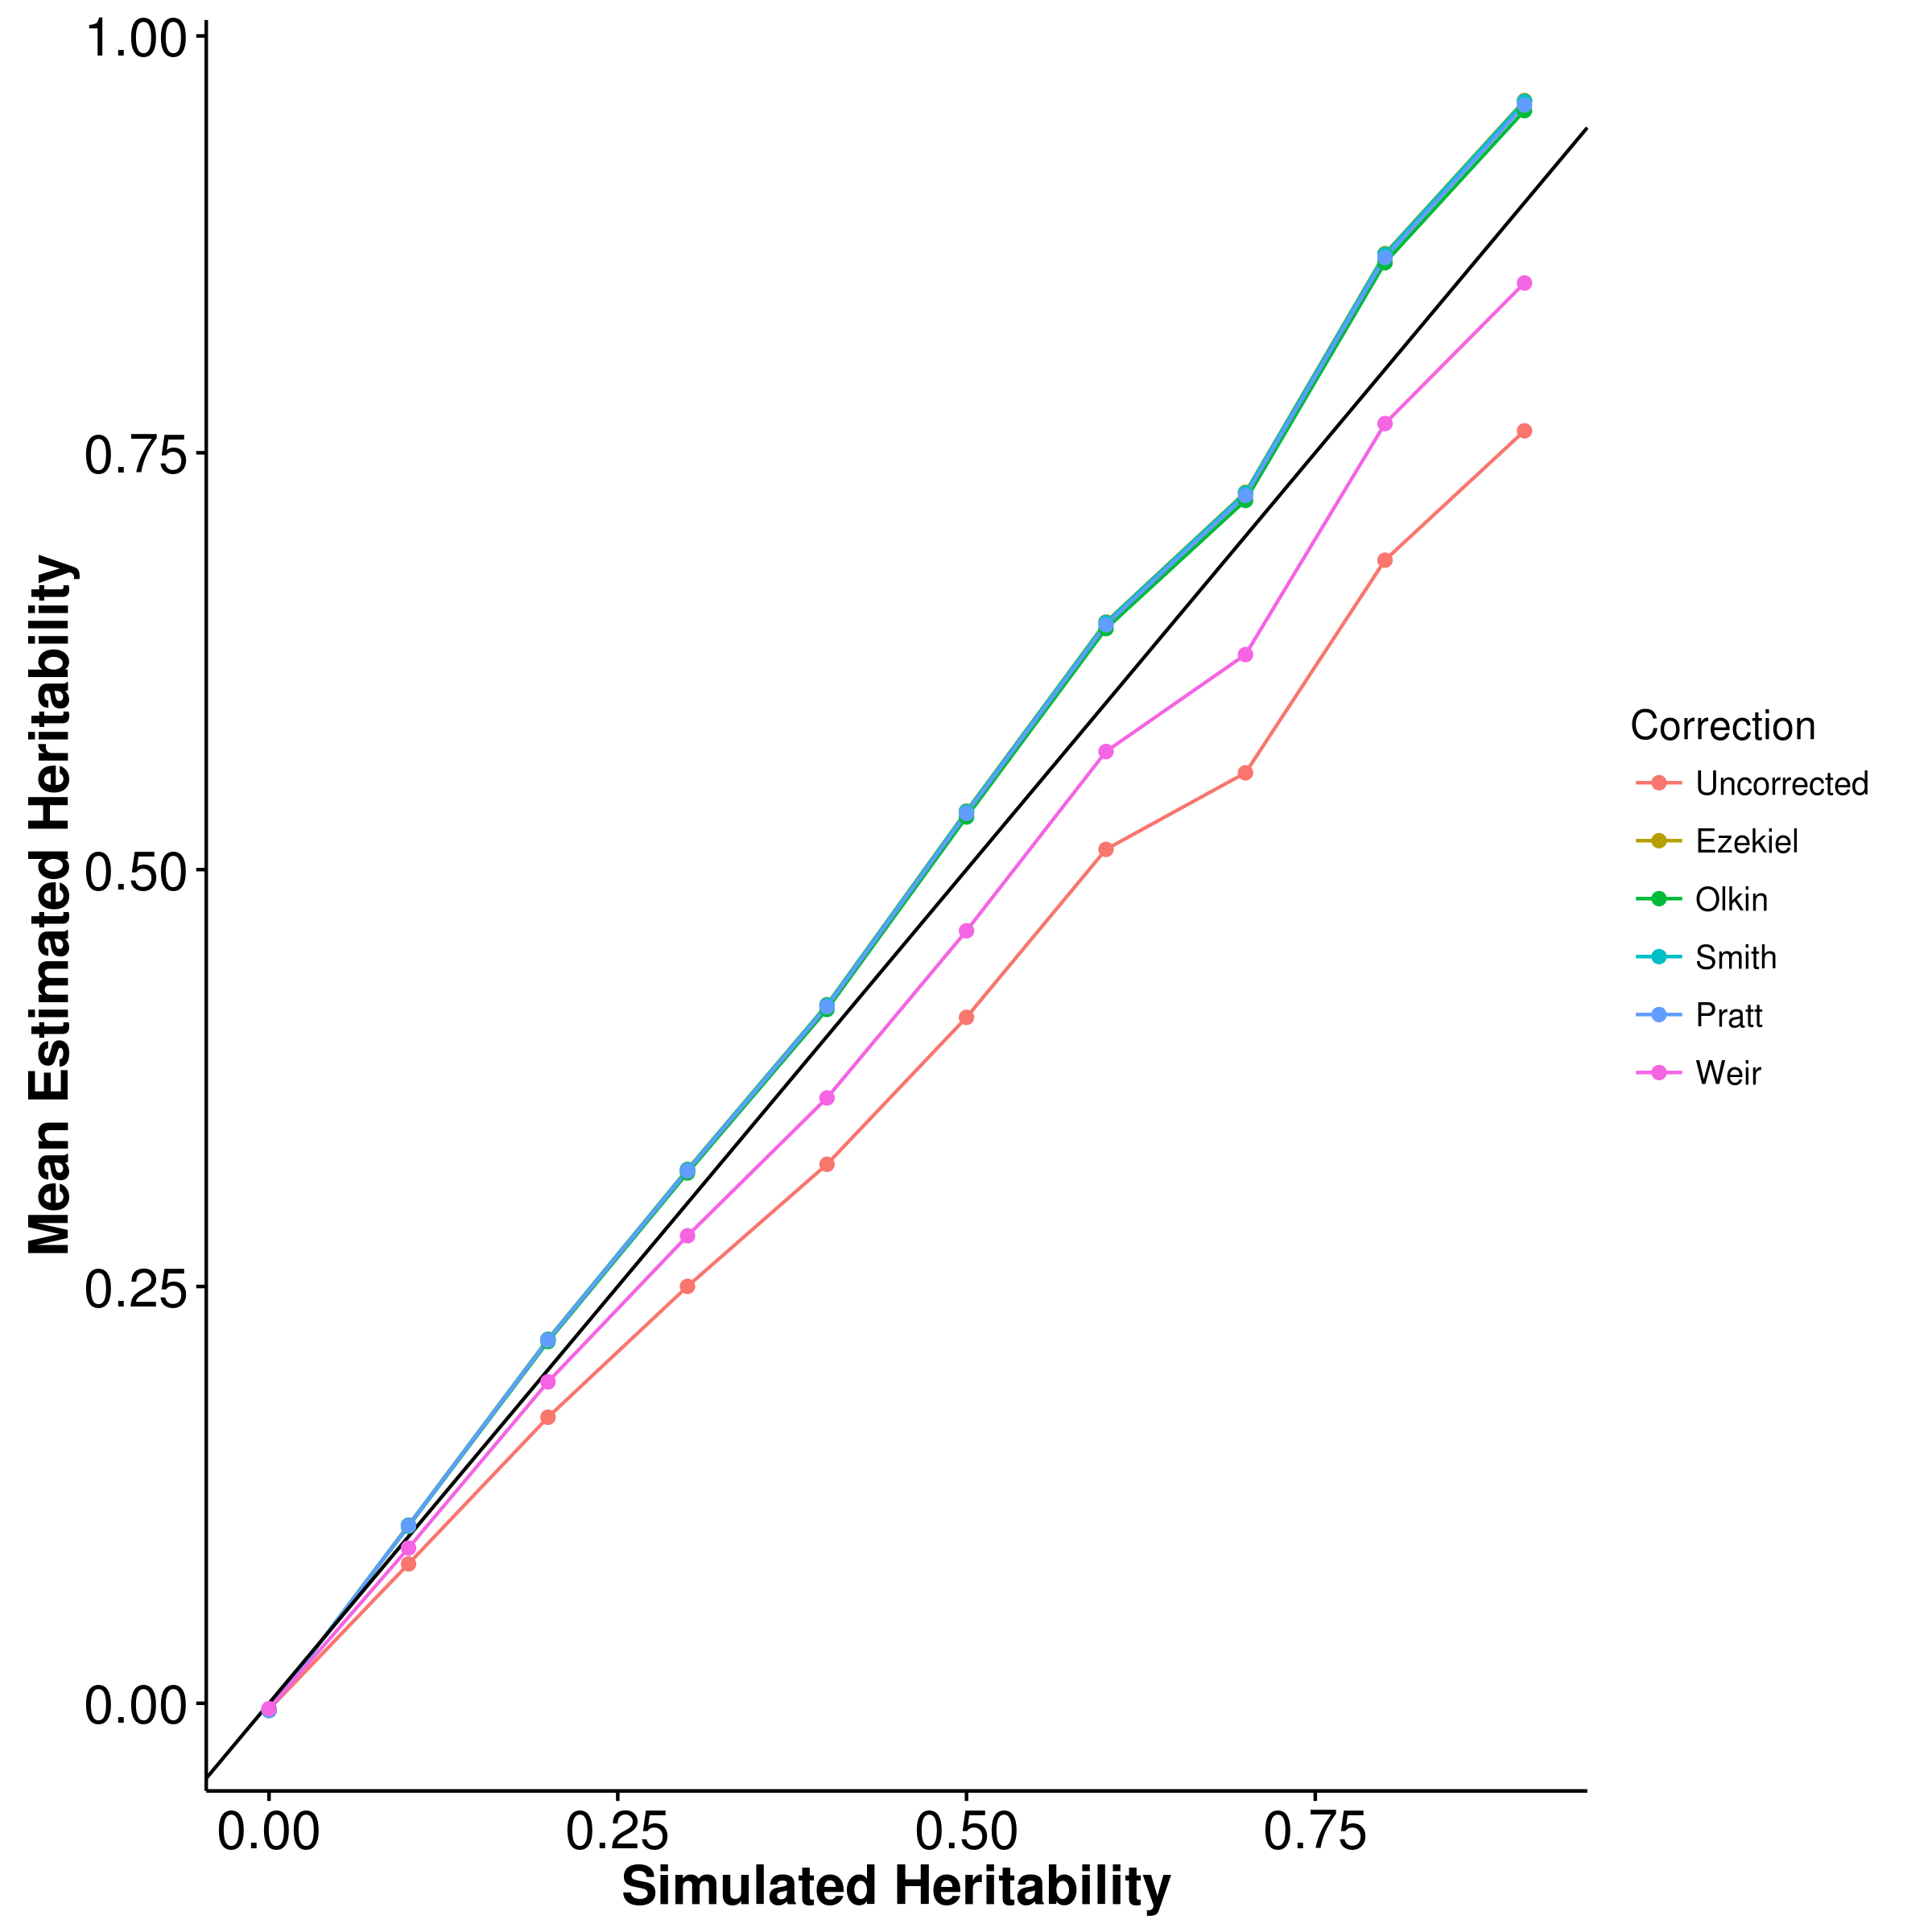
\includegraphics[width=0.5\textwidth]{figure/quantitative/ld_correct/LDCorrection_update.png}
	\caption[Effect of LD correction to Heritability Estimation]
	{Effect of LD correction to Heritability Estimation.
		We compared the performance of \gls{shrek} when different $R^2$ bias correction algorithm was used.
		When no bias correction was carried out, a downward bias was observed. 
		After the application of the bias correction algorithms, the mean estimations of all except in the case of Weir \cref{eq:weir} algorithms leads to an overestimation of heritability.
	} 
	\label{fig:meanLDCor}
\end{figure}
As \gls{shrek} relies on the \gls{LD} structure to estimate the \gls{SNP} heritability, it is important to correct for bias in the \gls{LD} estimates. 
The performance of the correct algorithms were tested through the HAPGEN2 simulation (\cref{fig:meanLDCor}).
It is observed that when no bias correction was applied, the mean estimates biased downward, as expected.

The main purpose of this simulation is to test how the \gls{LD} correction methods affect the performance of \gls{shrek}.
With the exception of the formula proposed by \citet{Weir1980} (\cref{eq:weir}), all correction methods results in estimates that are upwardly biased.
We hypothesize that it might be because of ``over-adjustment'' by these method, therefore lead to an inflated estimates.
Given these results, it is concluded that \citet{Weir1980}'s formula has the best performance and are therefore selected as the default \gls{LD} correction algorithm for \gls{shrek}.

\subsection{Simulation Study}
To formally assess the performance of \gls{ldsc} and \gls{shrek} under different scenarios, a number of simulations were performed.

\subsubsection{Quantitative Trait Simulation}
%Mean
\begin{figure}
	\centering
	\subfloat[SHREK]{
		\scalebox{.4}{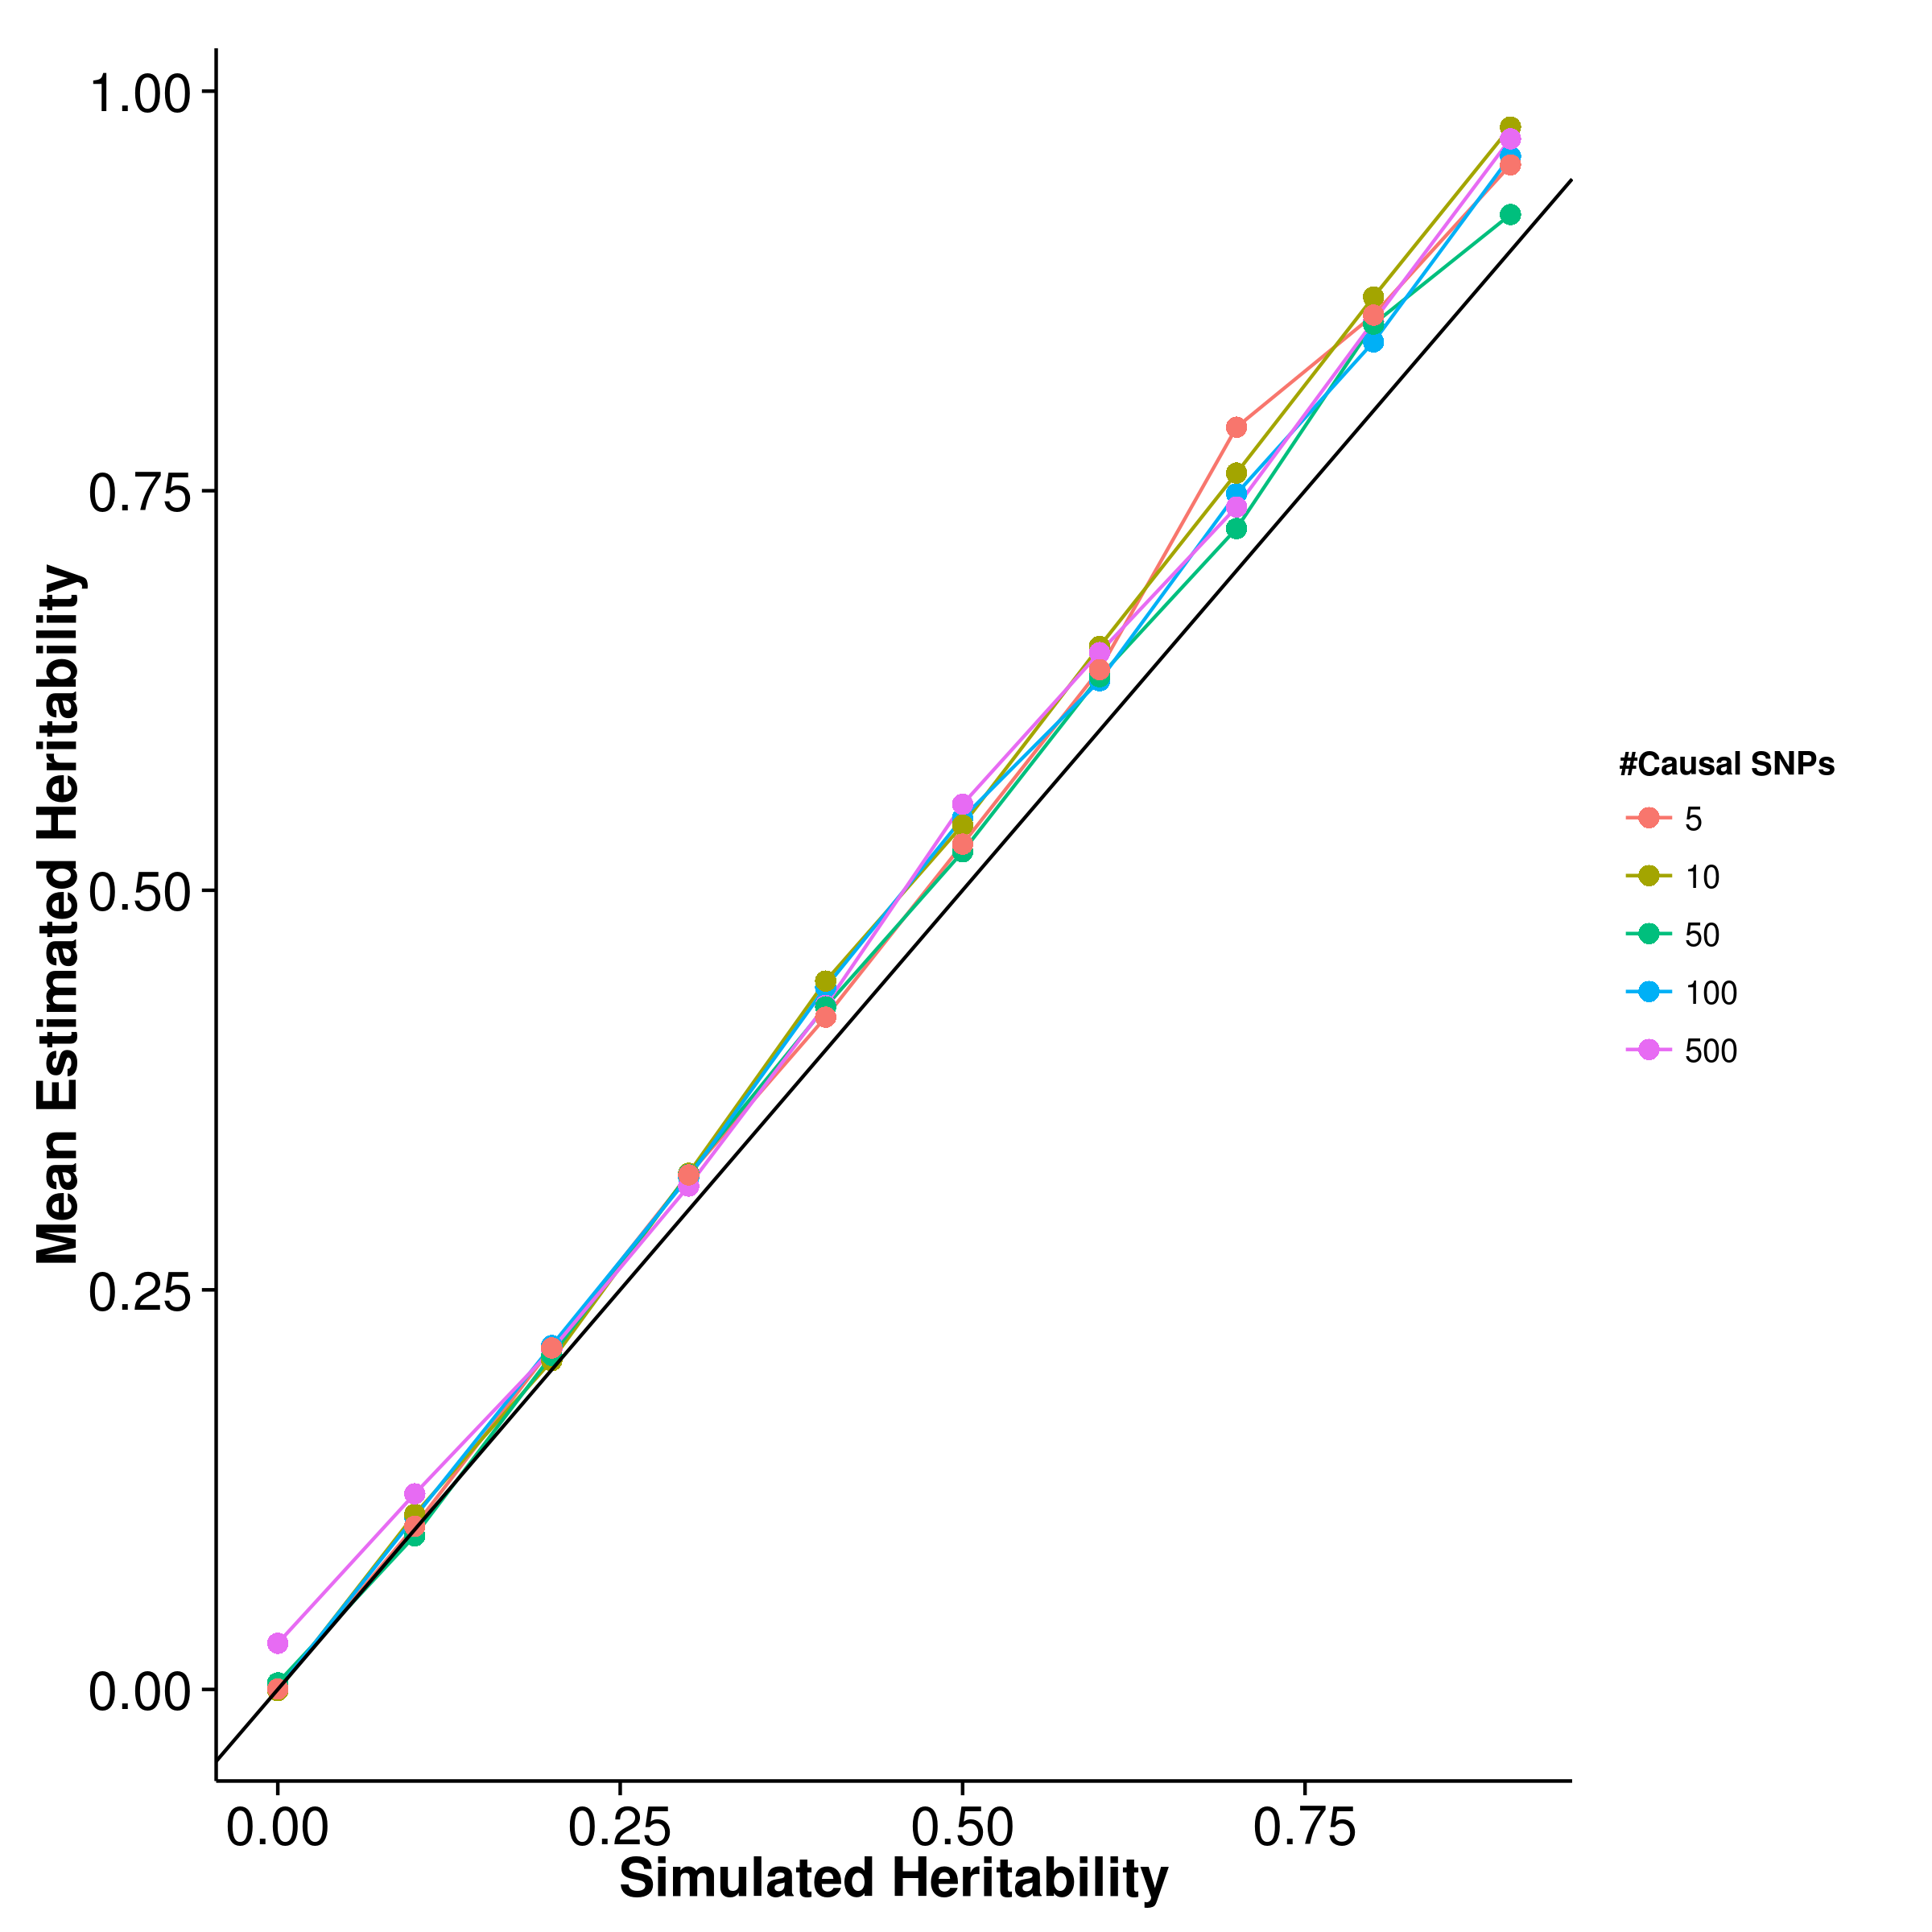
\includegraphics{figure/he_summary/random/shrek_Qt_Rand_mean.png}}
		\label{fig:shrekQtRandMean}
	}
	\subfloat[GCTA]{
		\scalebox{.4}{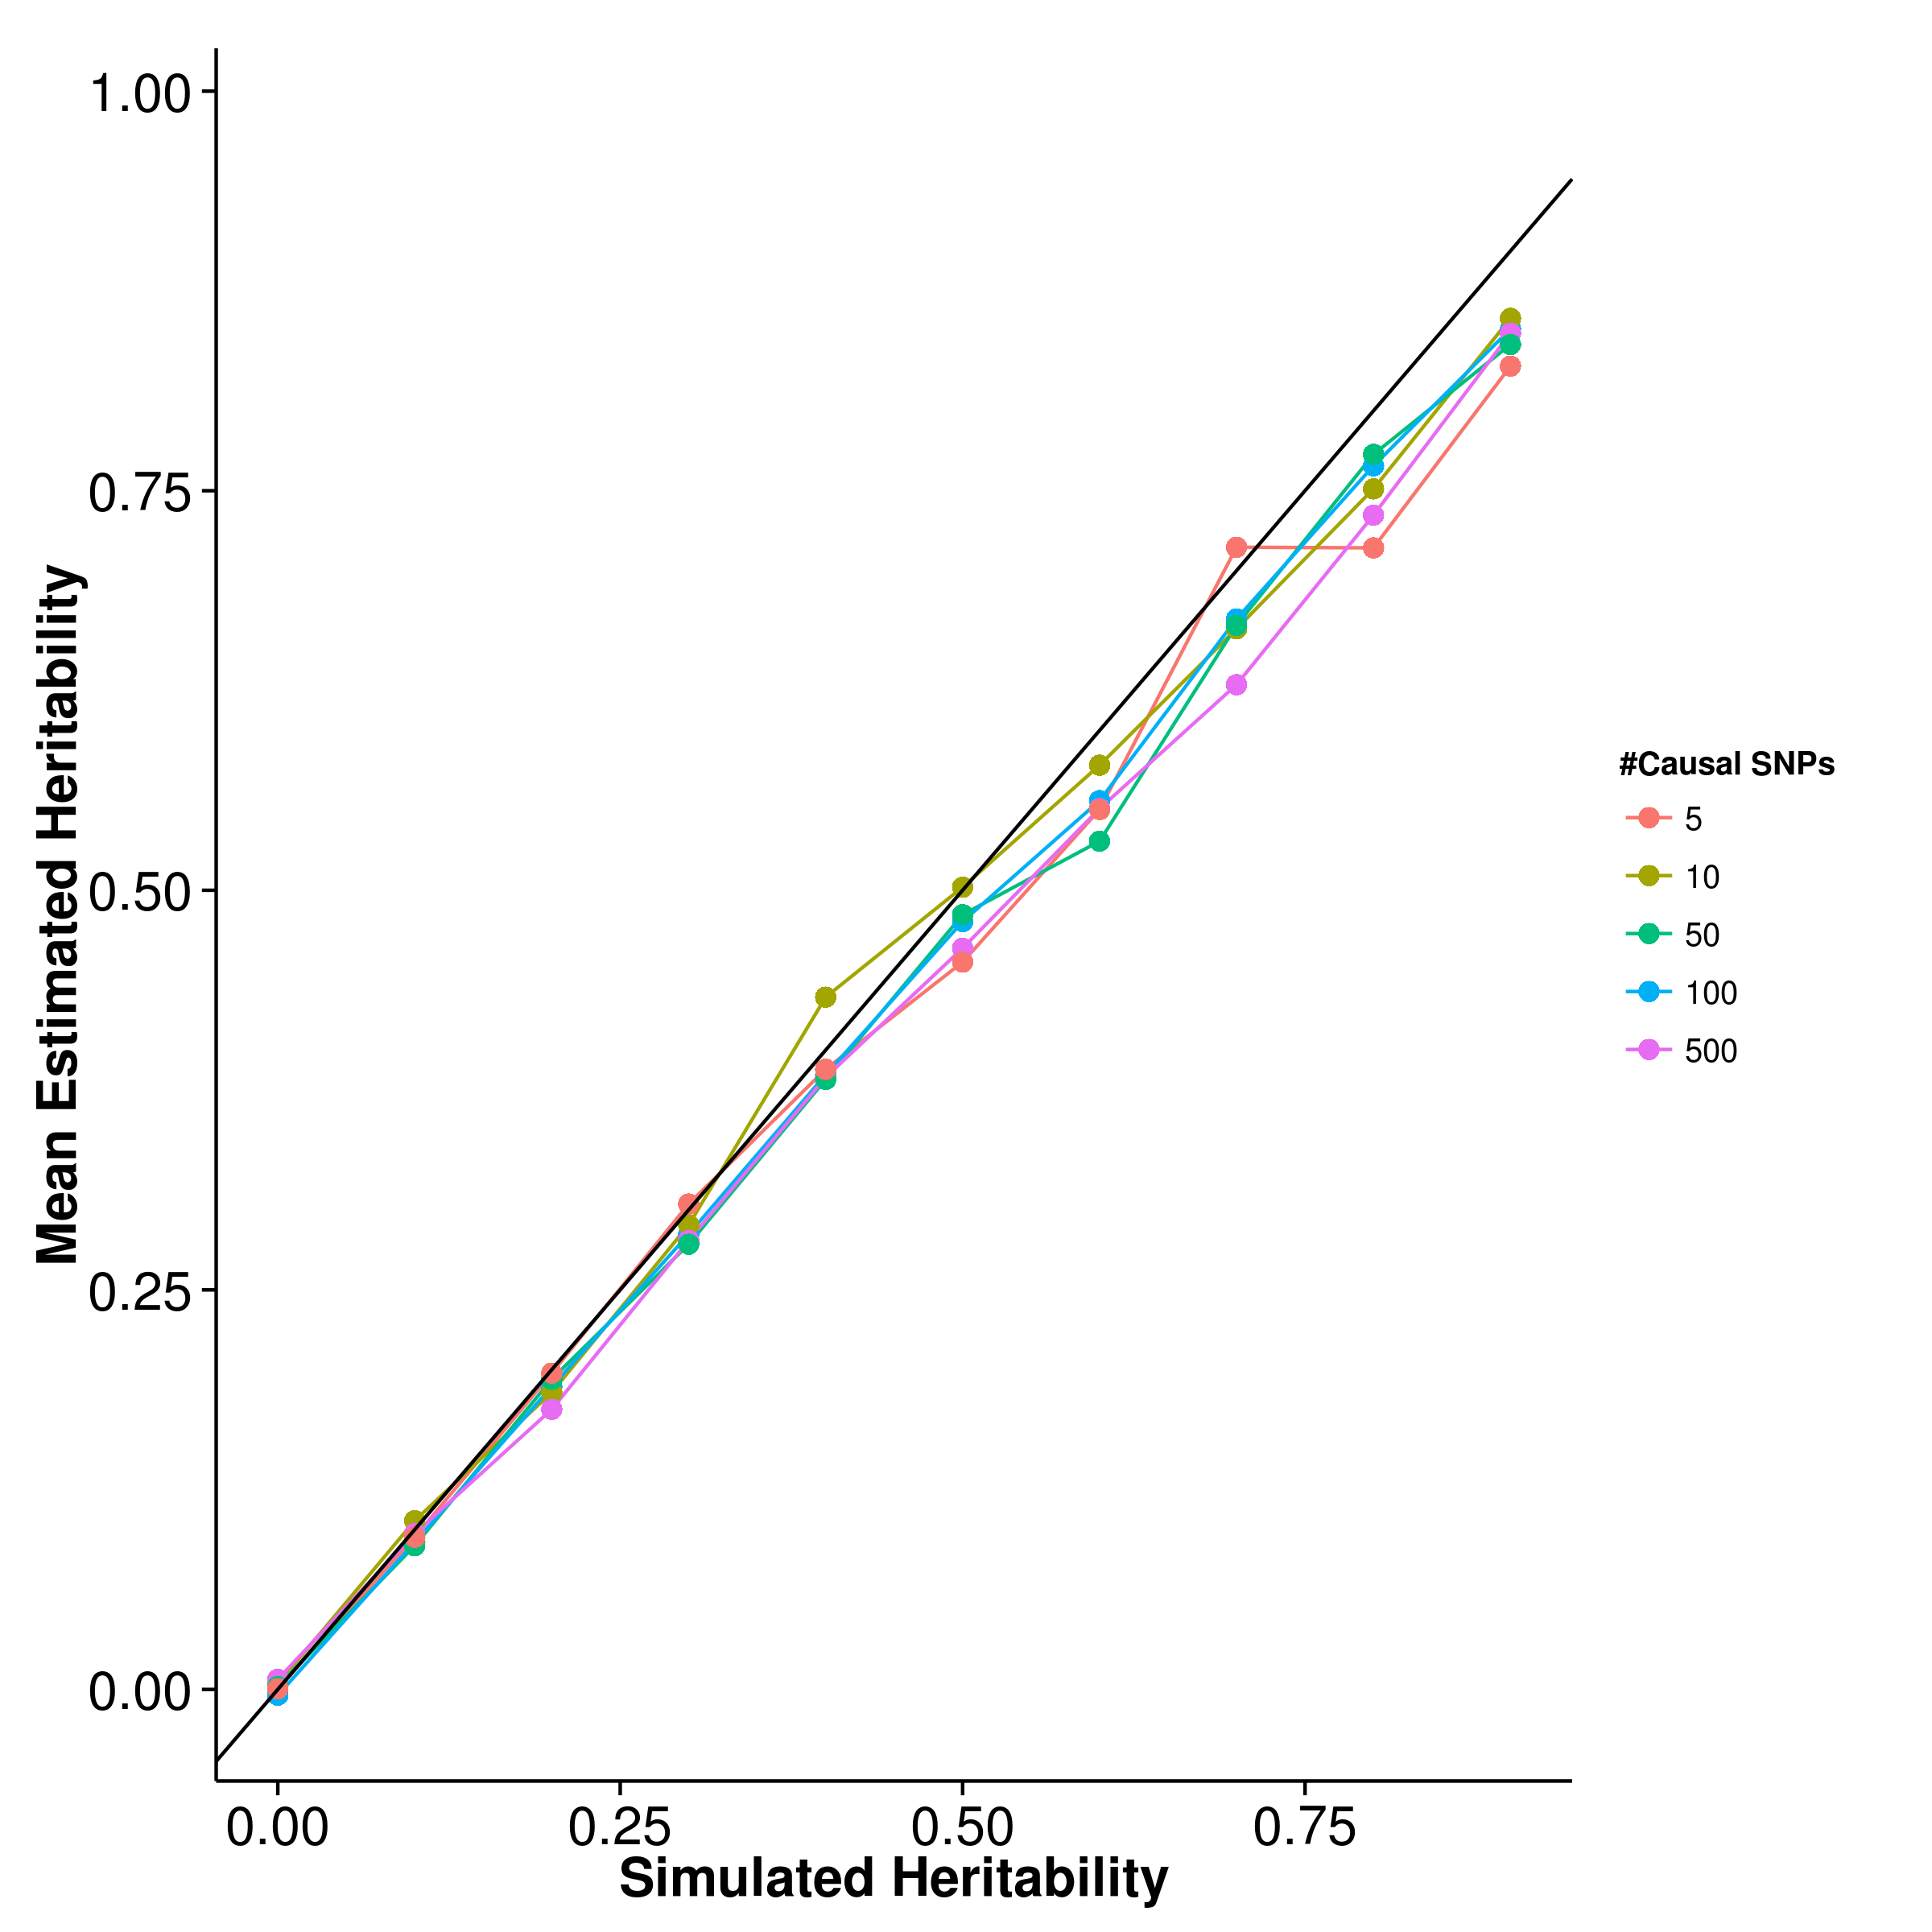
\includegraphics{figure/he_summary/random/gcta_Qt_Rand_mean.png}}
		\label{fig:gctaQtRandMean}
	}\\
	\subfloat[LDSC with fix intercept]{
		\scalebox{.4}{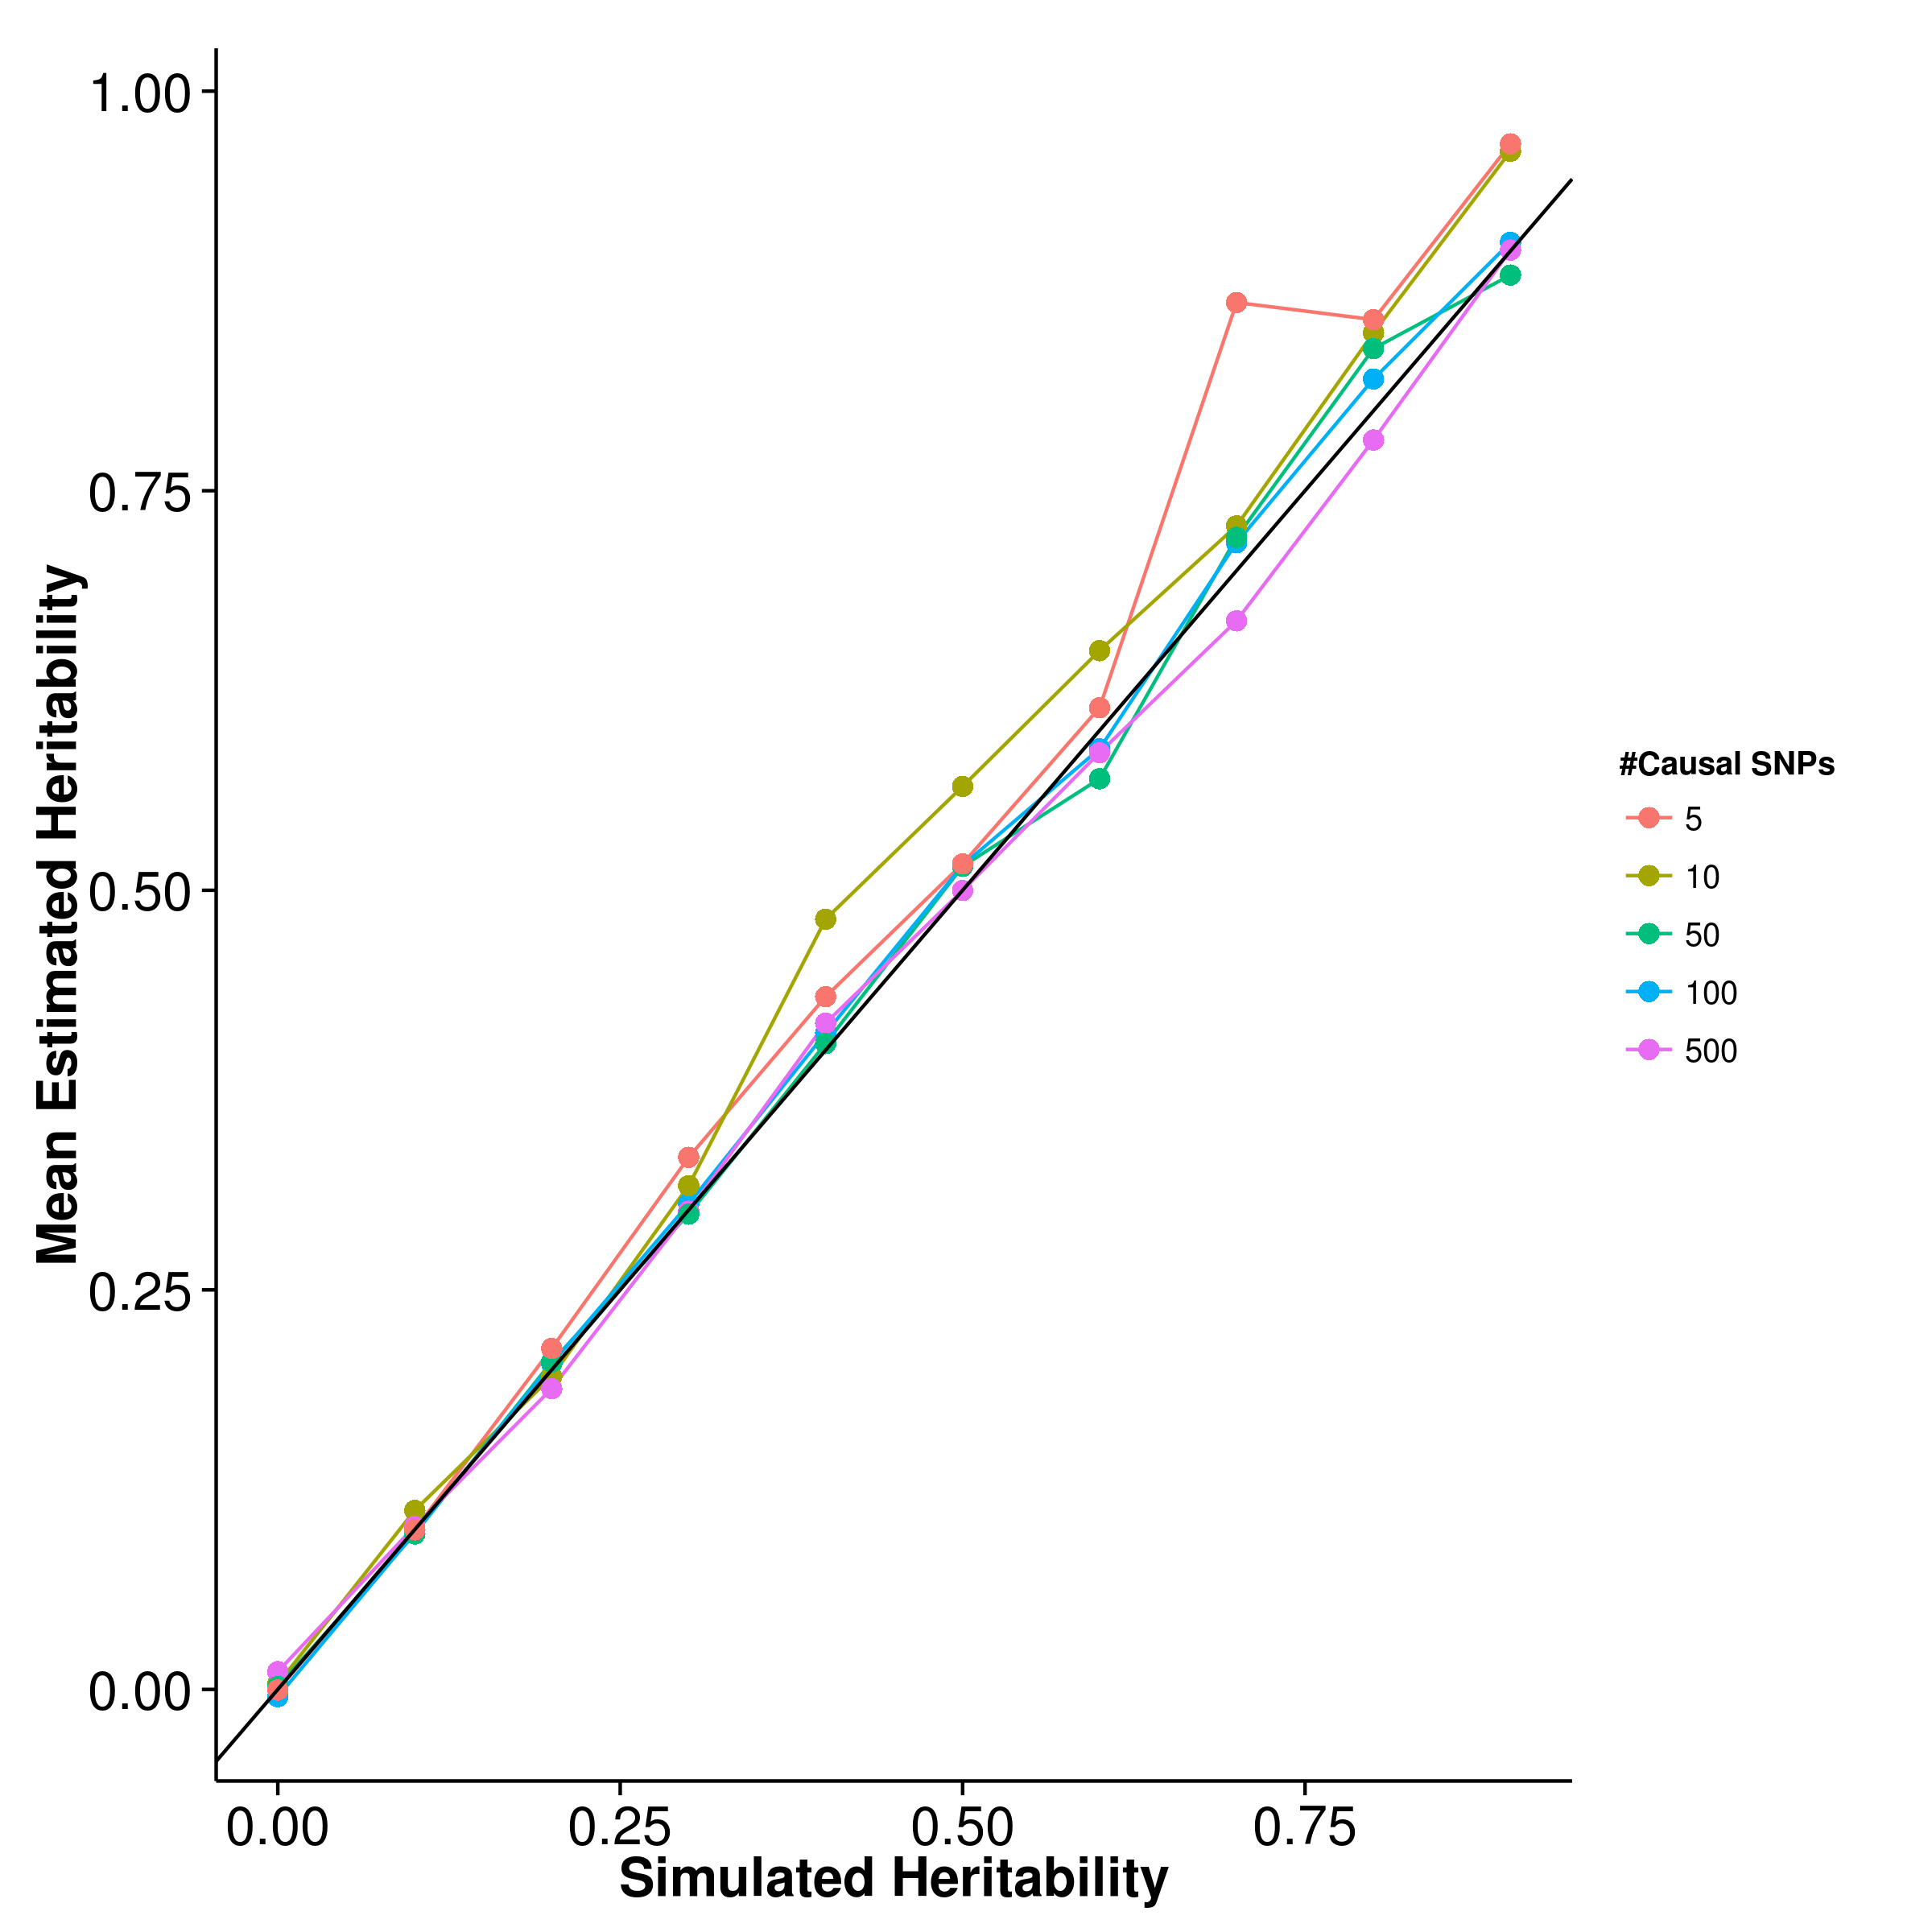
\includegraphics{figure/he_summary/random/ldsc_Qt_Rand_mean.png}}
		\label{fig:ldscQtRandMean}
	}
	\subfloat[LDSC with intercept estimation]{
		
		\scalebox{.4}{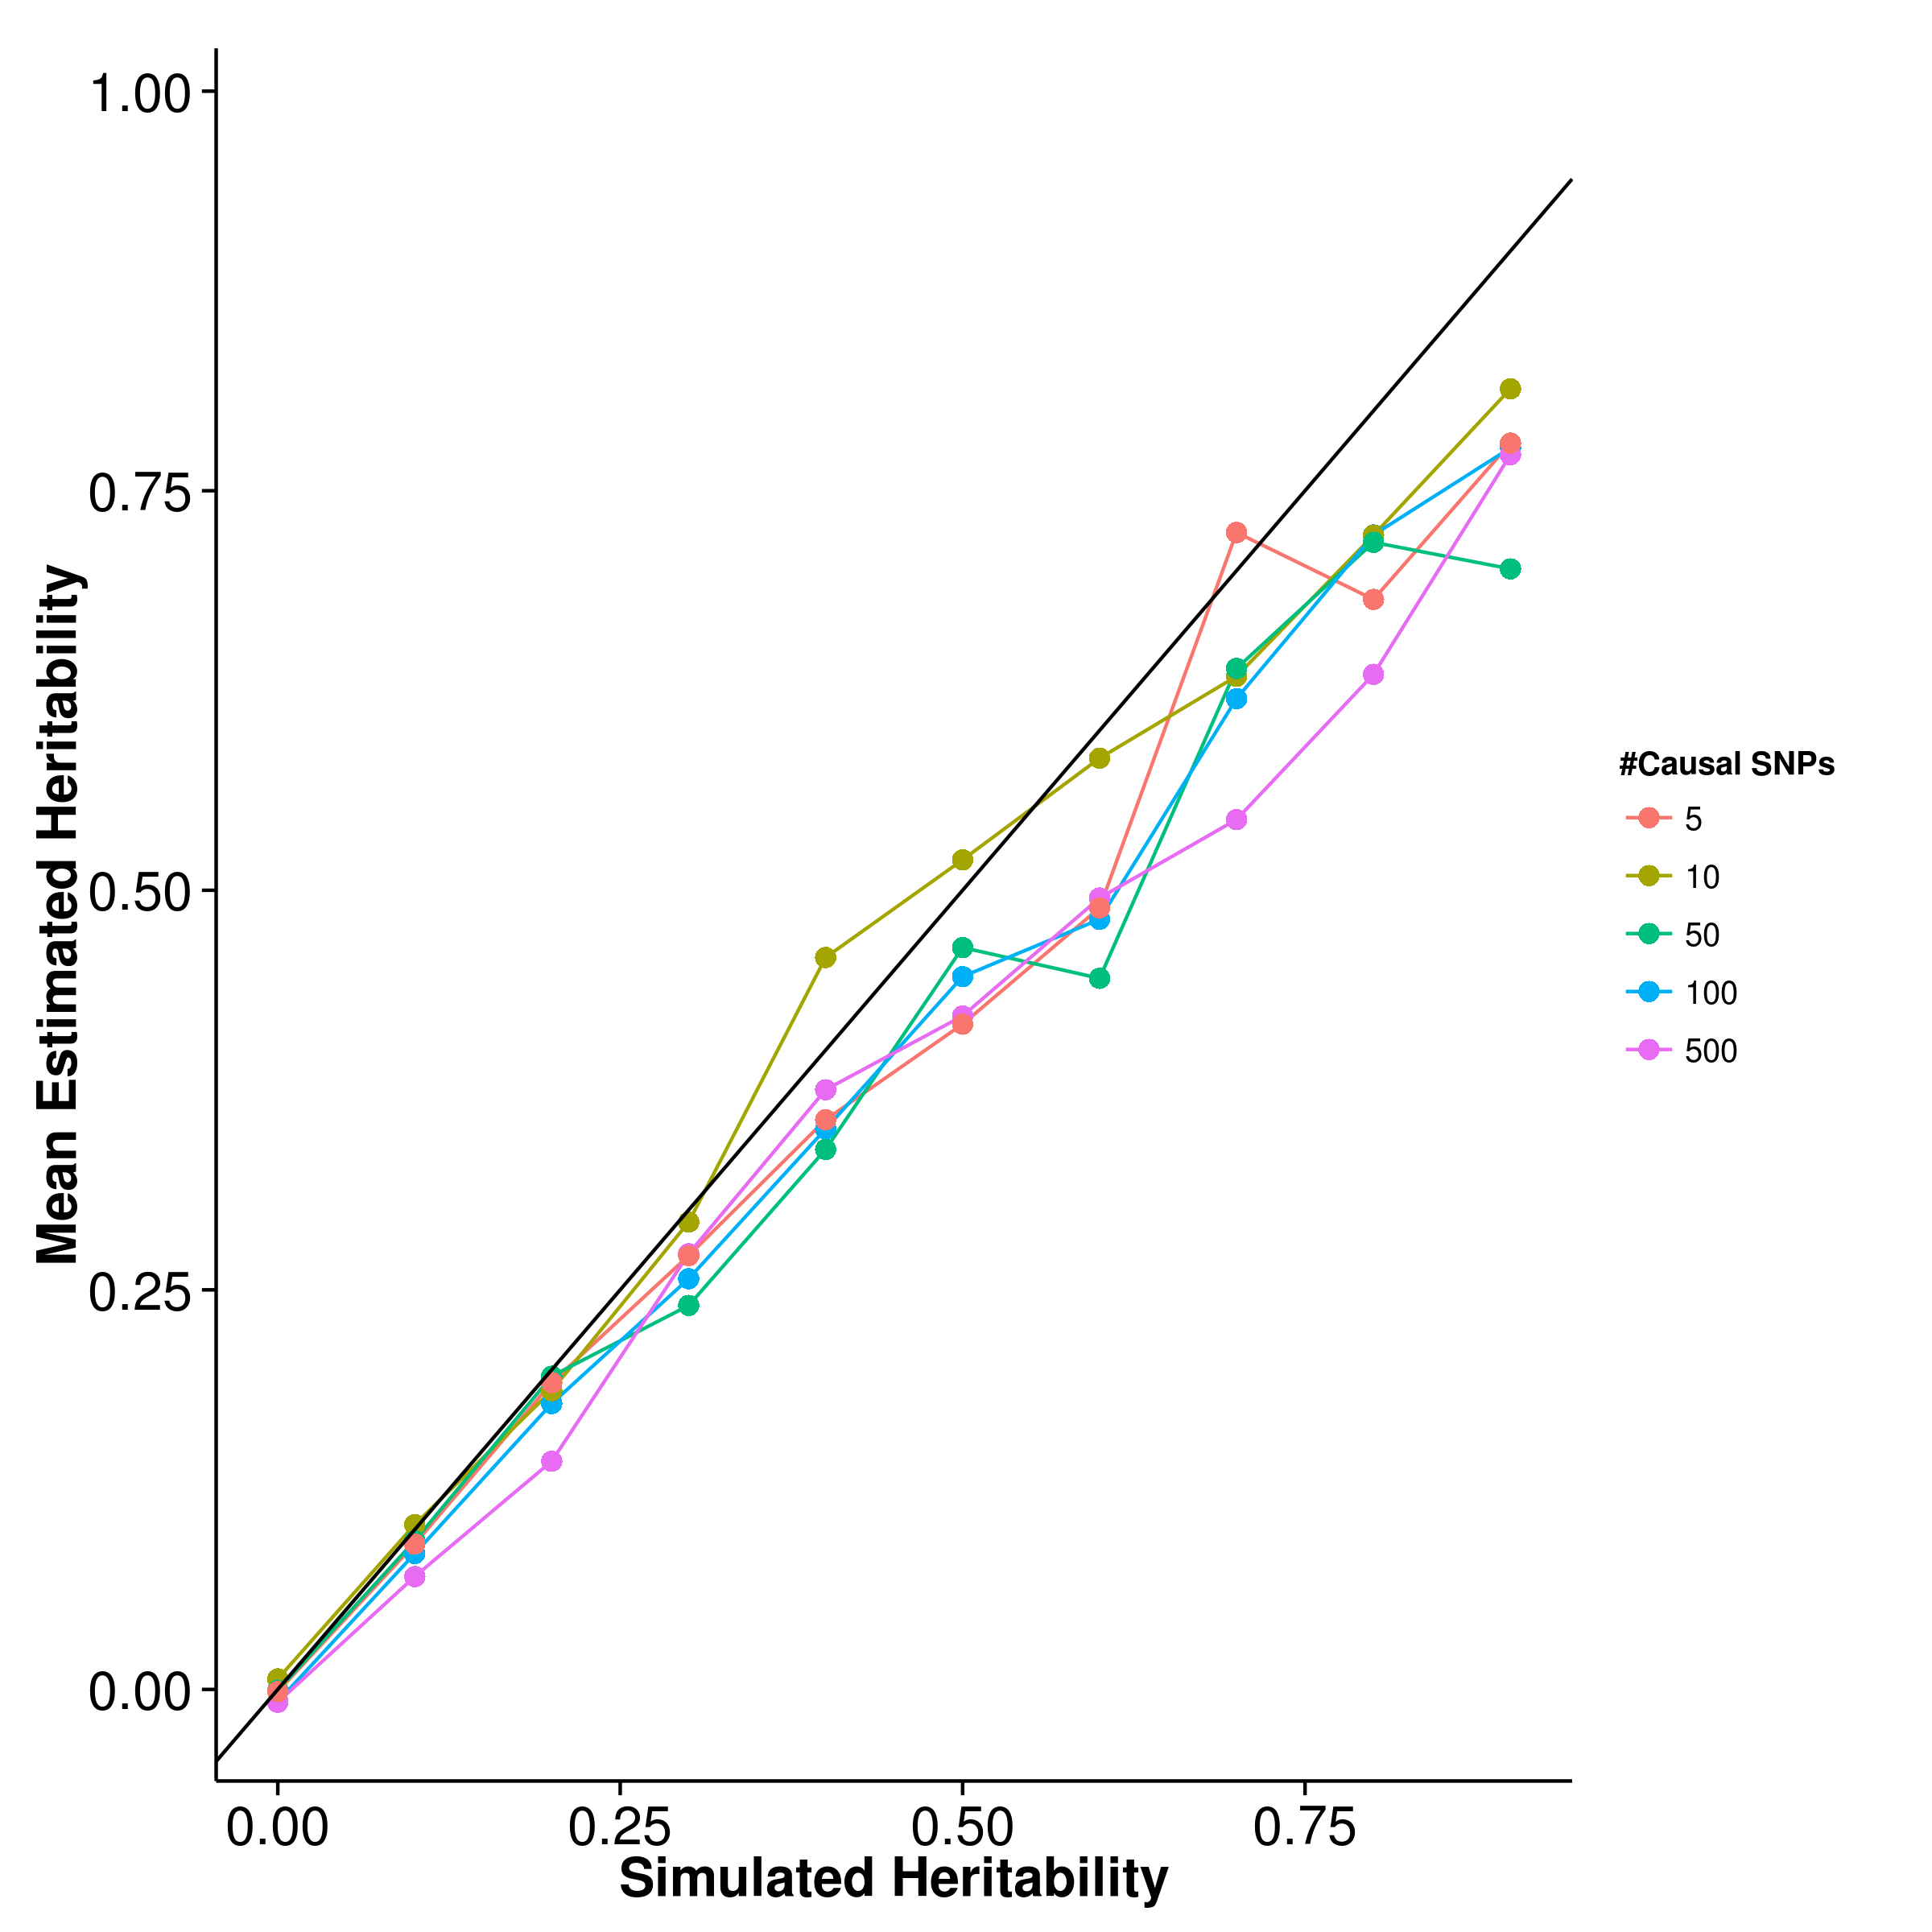
\includegraphics{figure/he_summary/random/ldscIn_Qt_Rand_mean.png}}
		\label{fig:ldscInQtRandMean}
	}
	\caption[Mean of Quantitative Trait Simulation Results]
	{Mean of results from quantitative trait simulation with random effect size simulation.
		Estimations form \gls{shrek} were slightly biased upwards whereas \gls{gcta} and \gls{ldsc} with intercept estimations both biased downwards.
		On the other hand, \gls{ldsc} with fixed intercept provides least biased estimates under polygenic conditions. 
		However, when the number of causal \glspl{SNP} is small (e.g. 5 or 10), an upward bias was observed.} 
	\label{fig:QtRandMean}
\end{figure}
%Variance
\begin{figure}
	\centering
	\subfloat[SHREK]{
		\scalebox{.4}{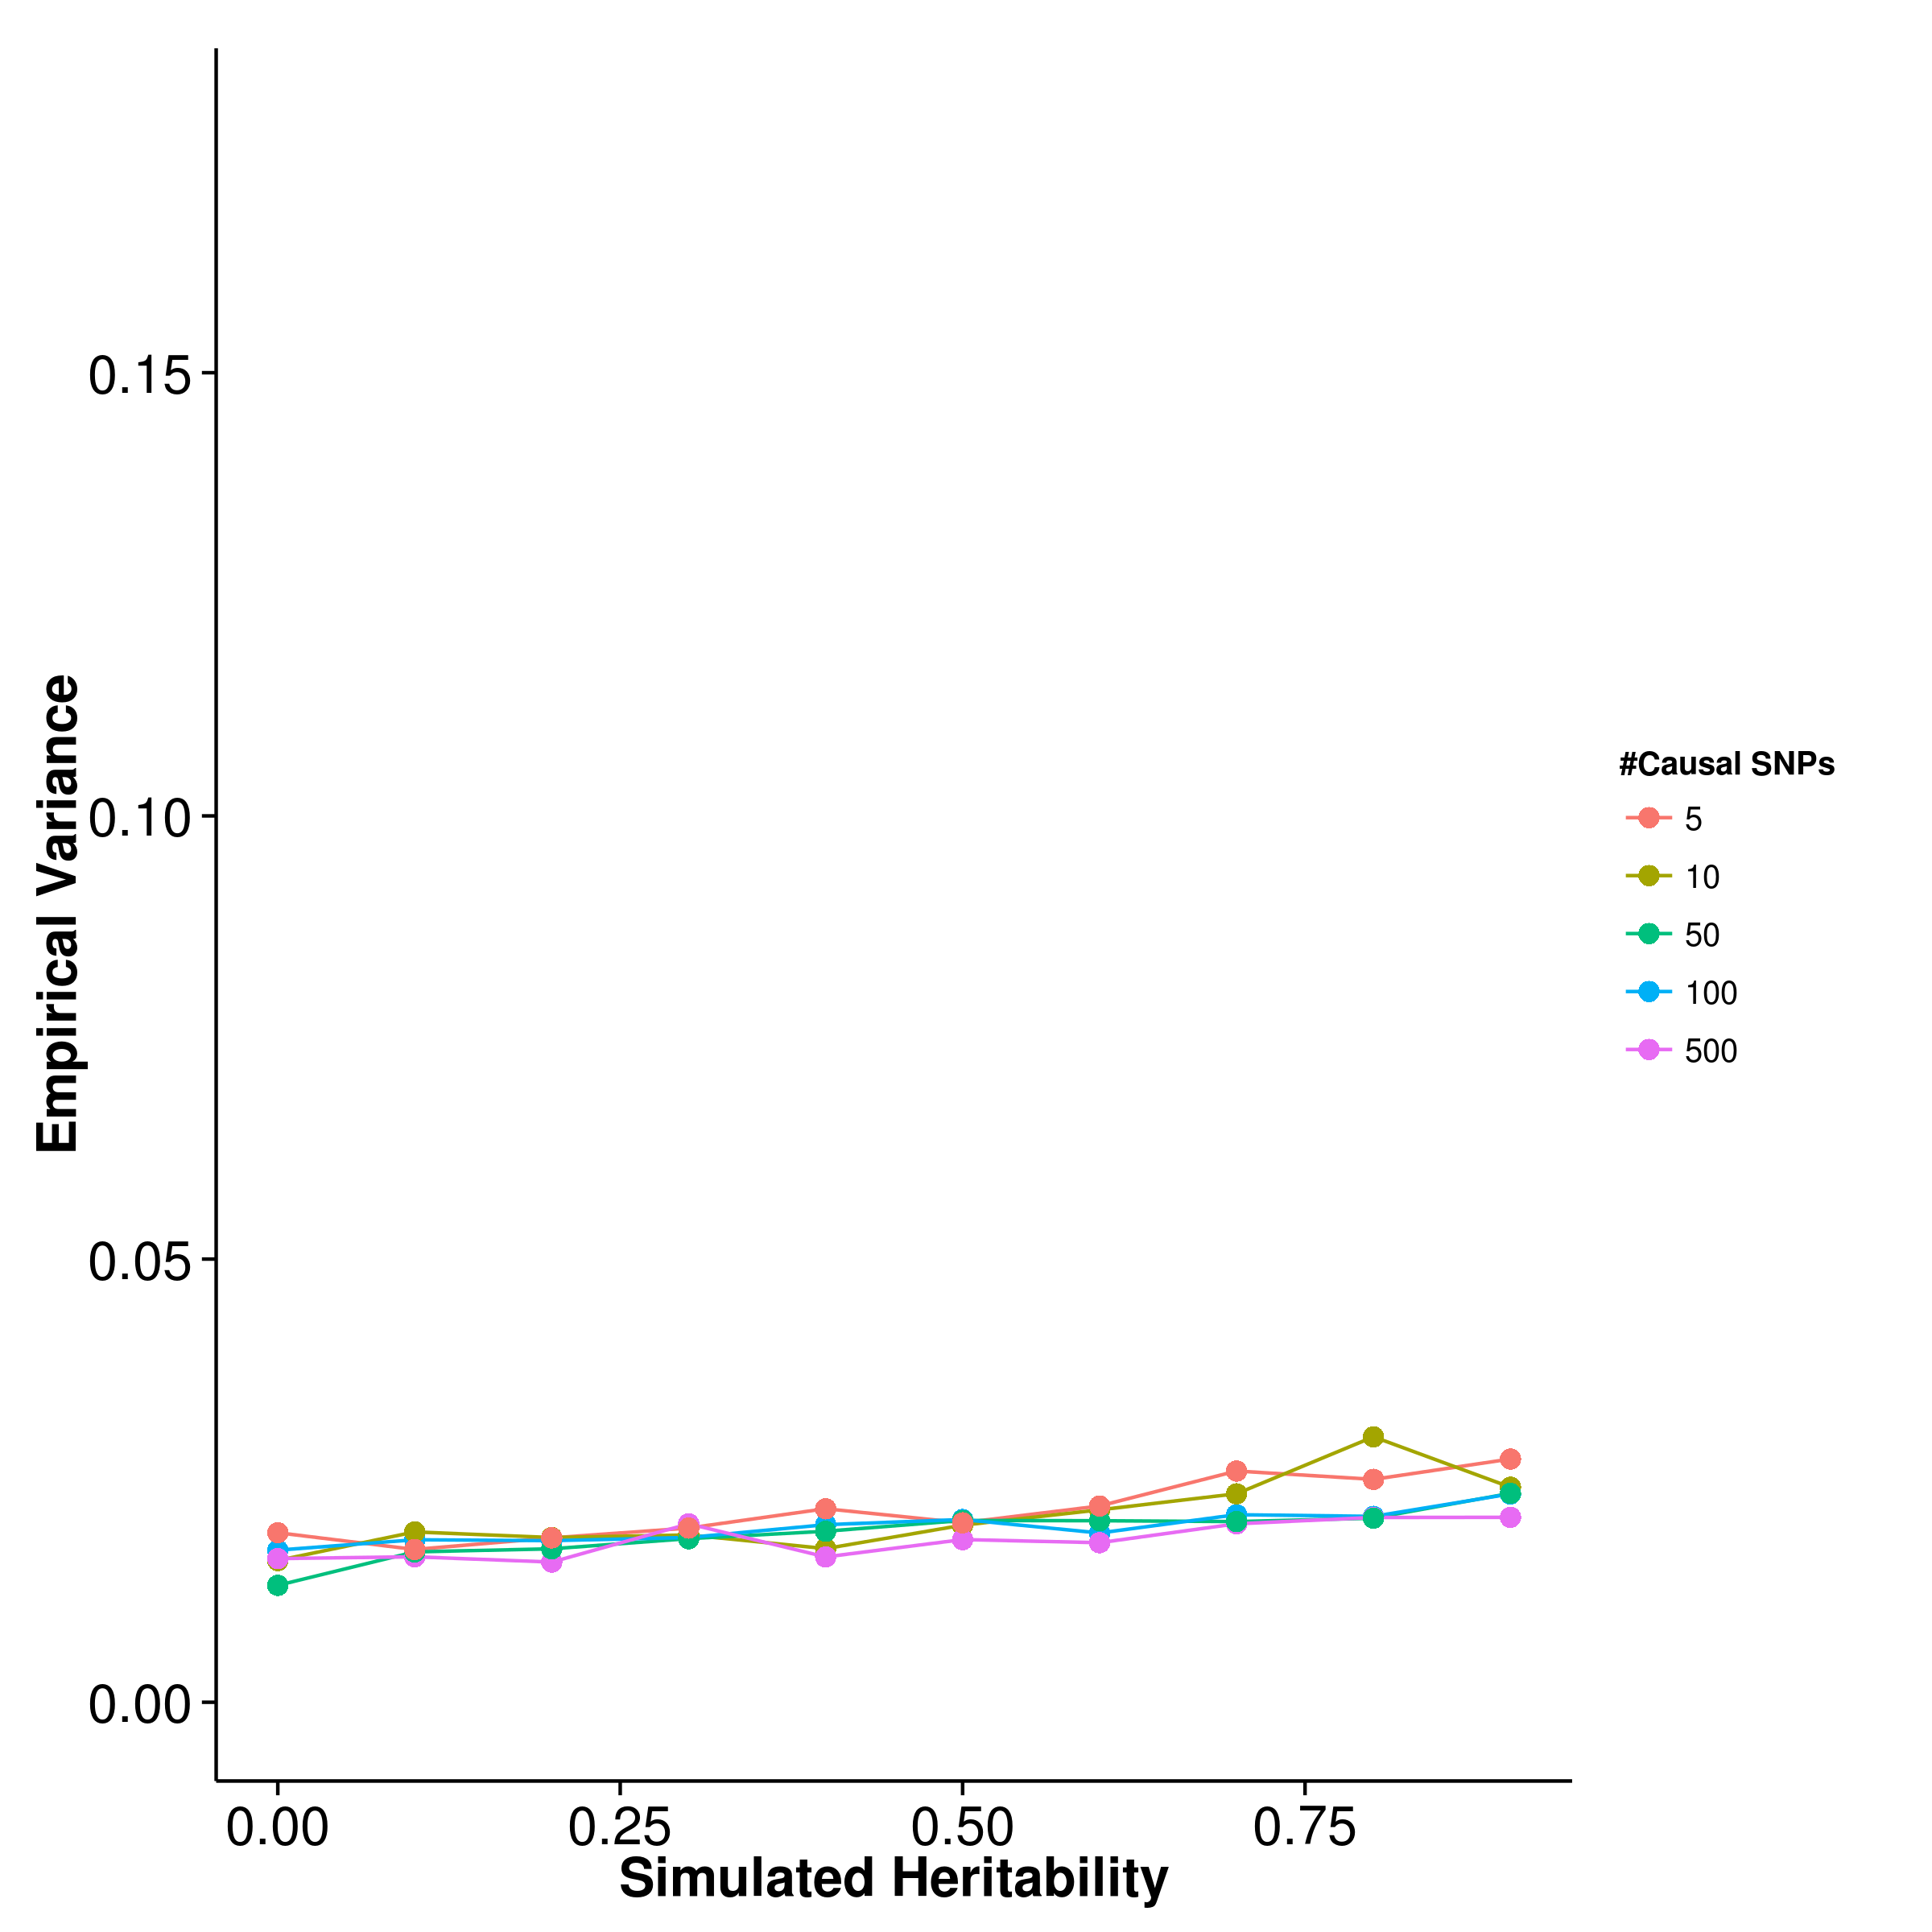
\includegraphics{figure/he_summary/random/shrek_Qt_Rand_sd.png}}
		\label{fig:shrekQtRandVar}
	}
	\subfloat[GCTA]{
		\scalebox{.4}{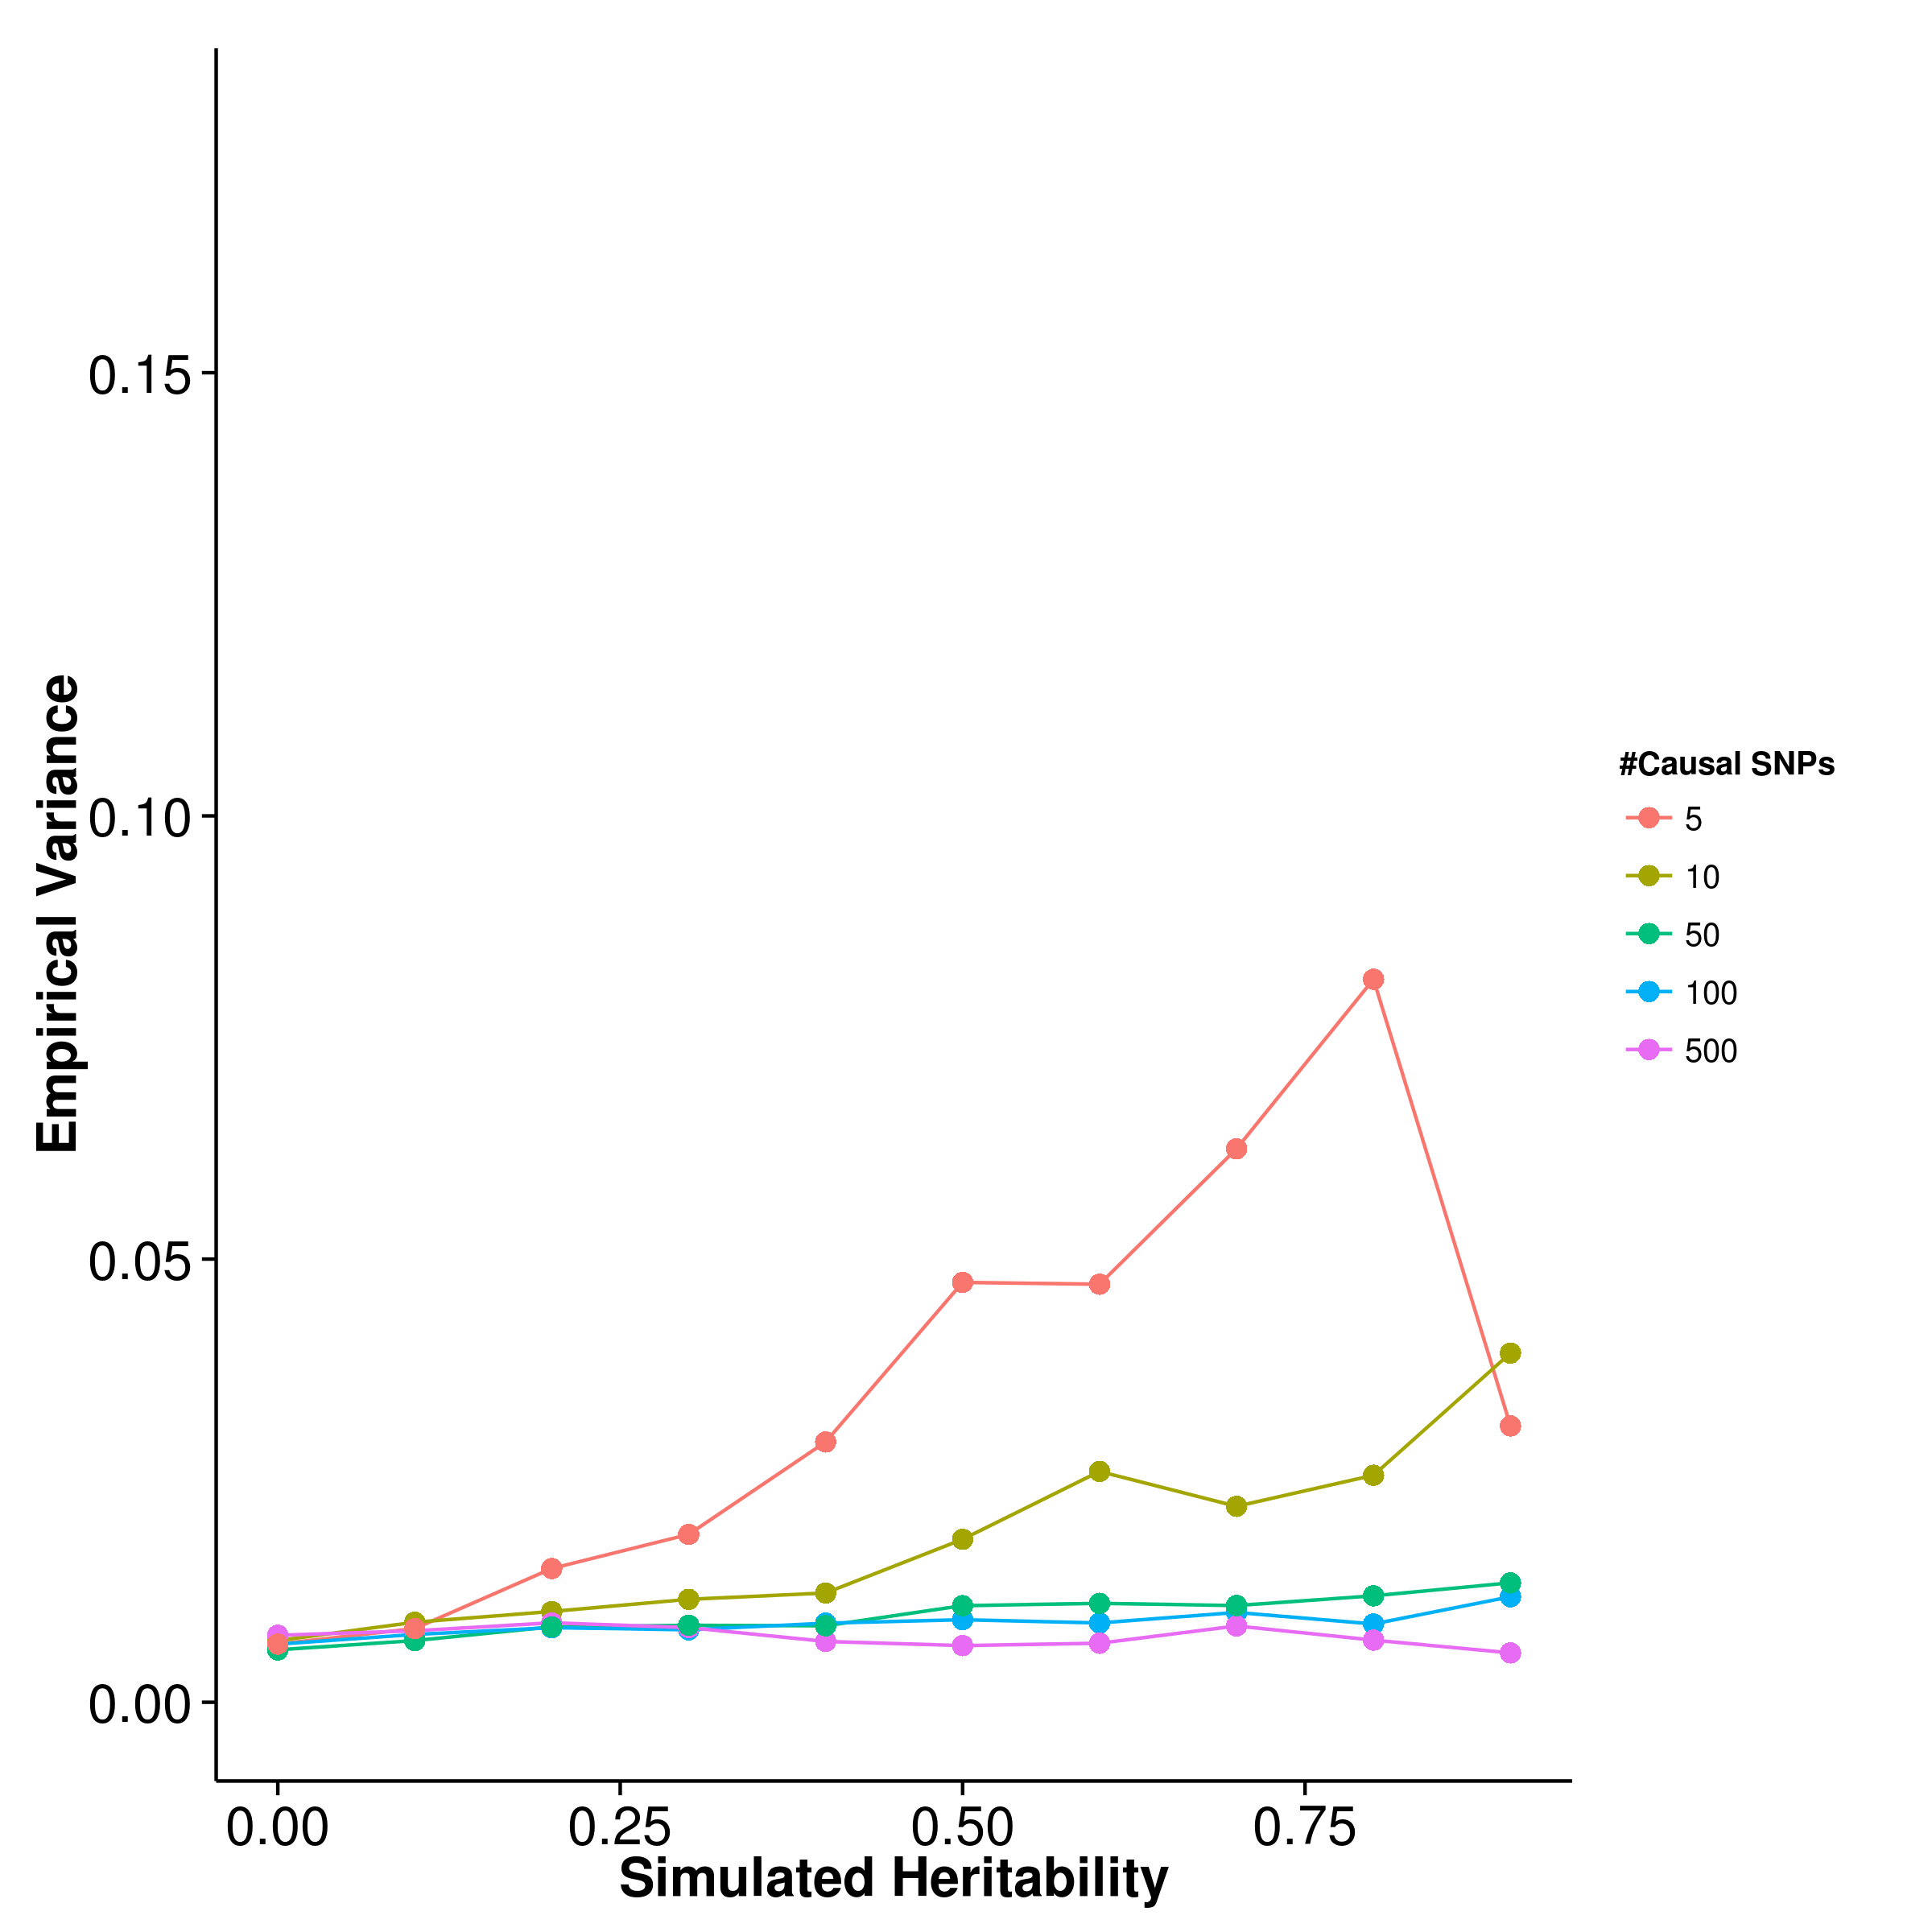
\includegraphics{figure/he_summary/random/gcta_Qt_Rand_sd.png}}
		\label{fig:gctaQtRandVar}
	}\\
	\subfloat[LDSC with fix intercept]{
		\scalebox{.4}{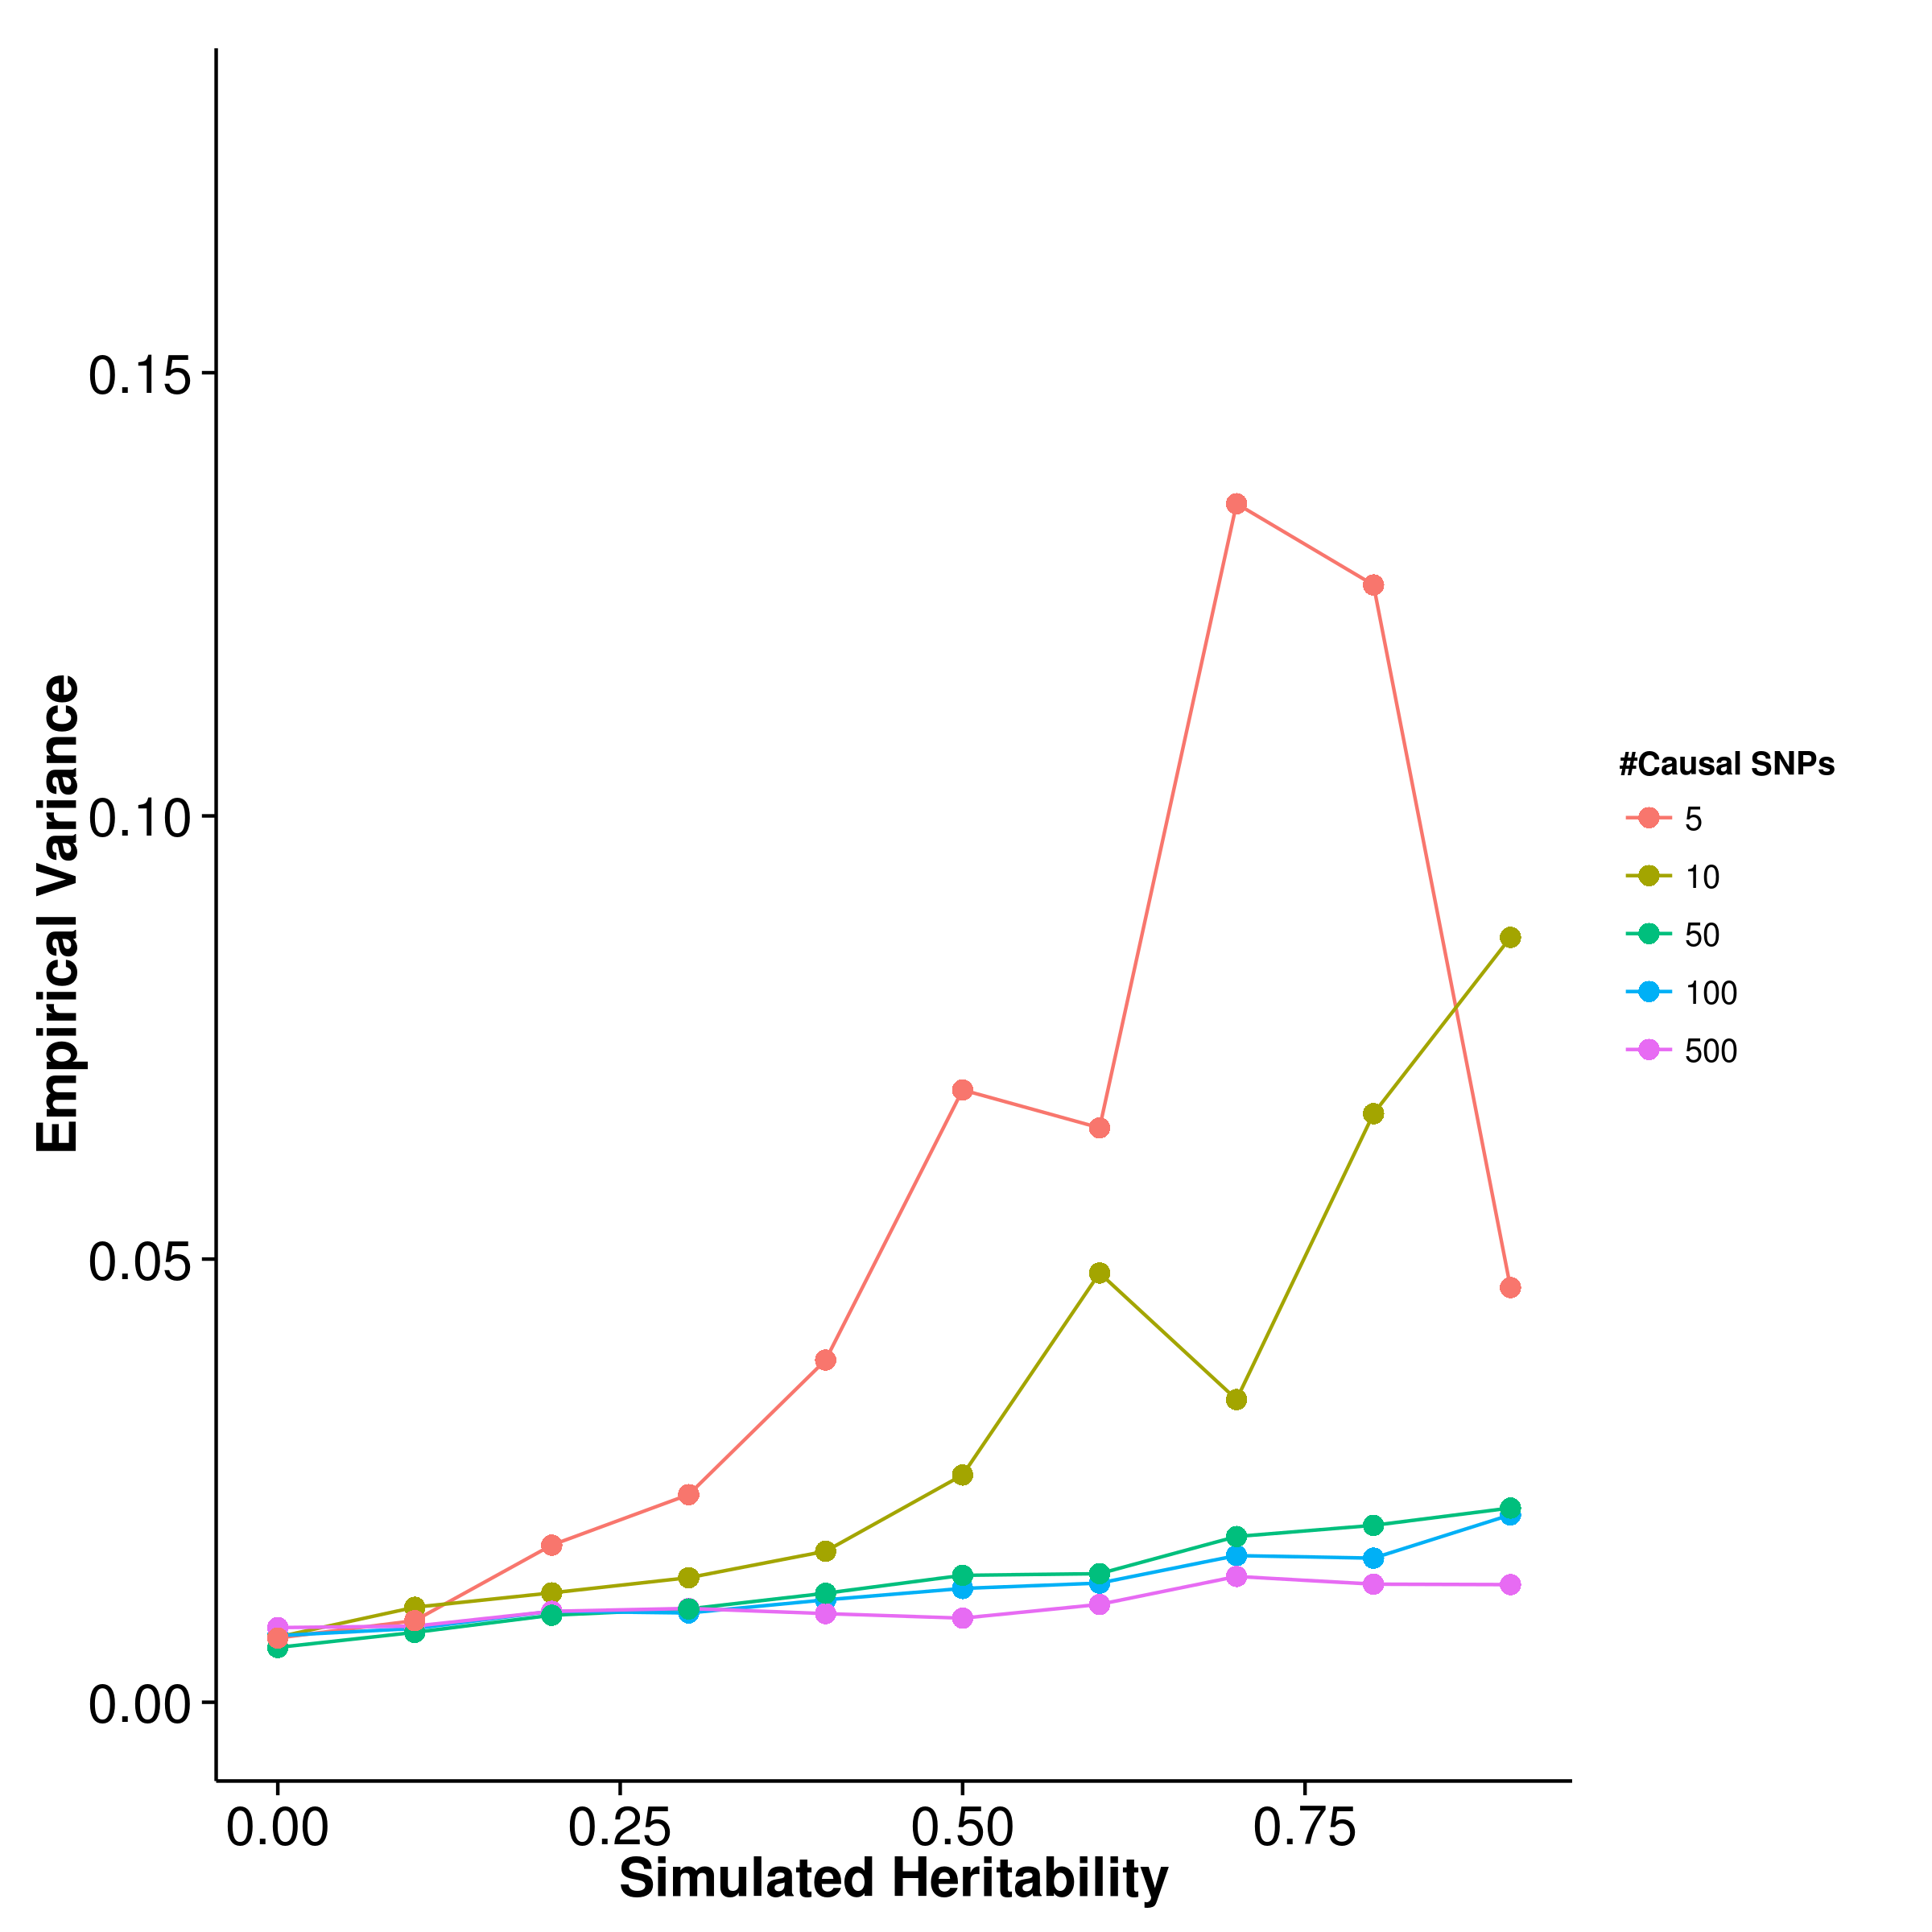
\includegraphics{figure/he_summary/random/ldsc_Qt_Rand_sd.png}}
		\label{fig:ldscQtRandVar}
	}
	\subfloat[LDSC with intercept estimation]{
		
		\scalebox{.4}{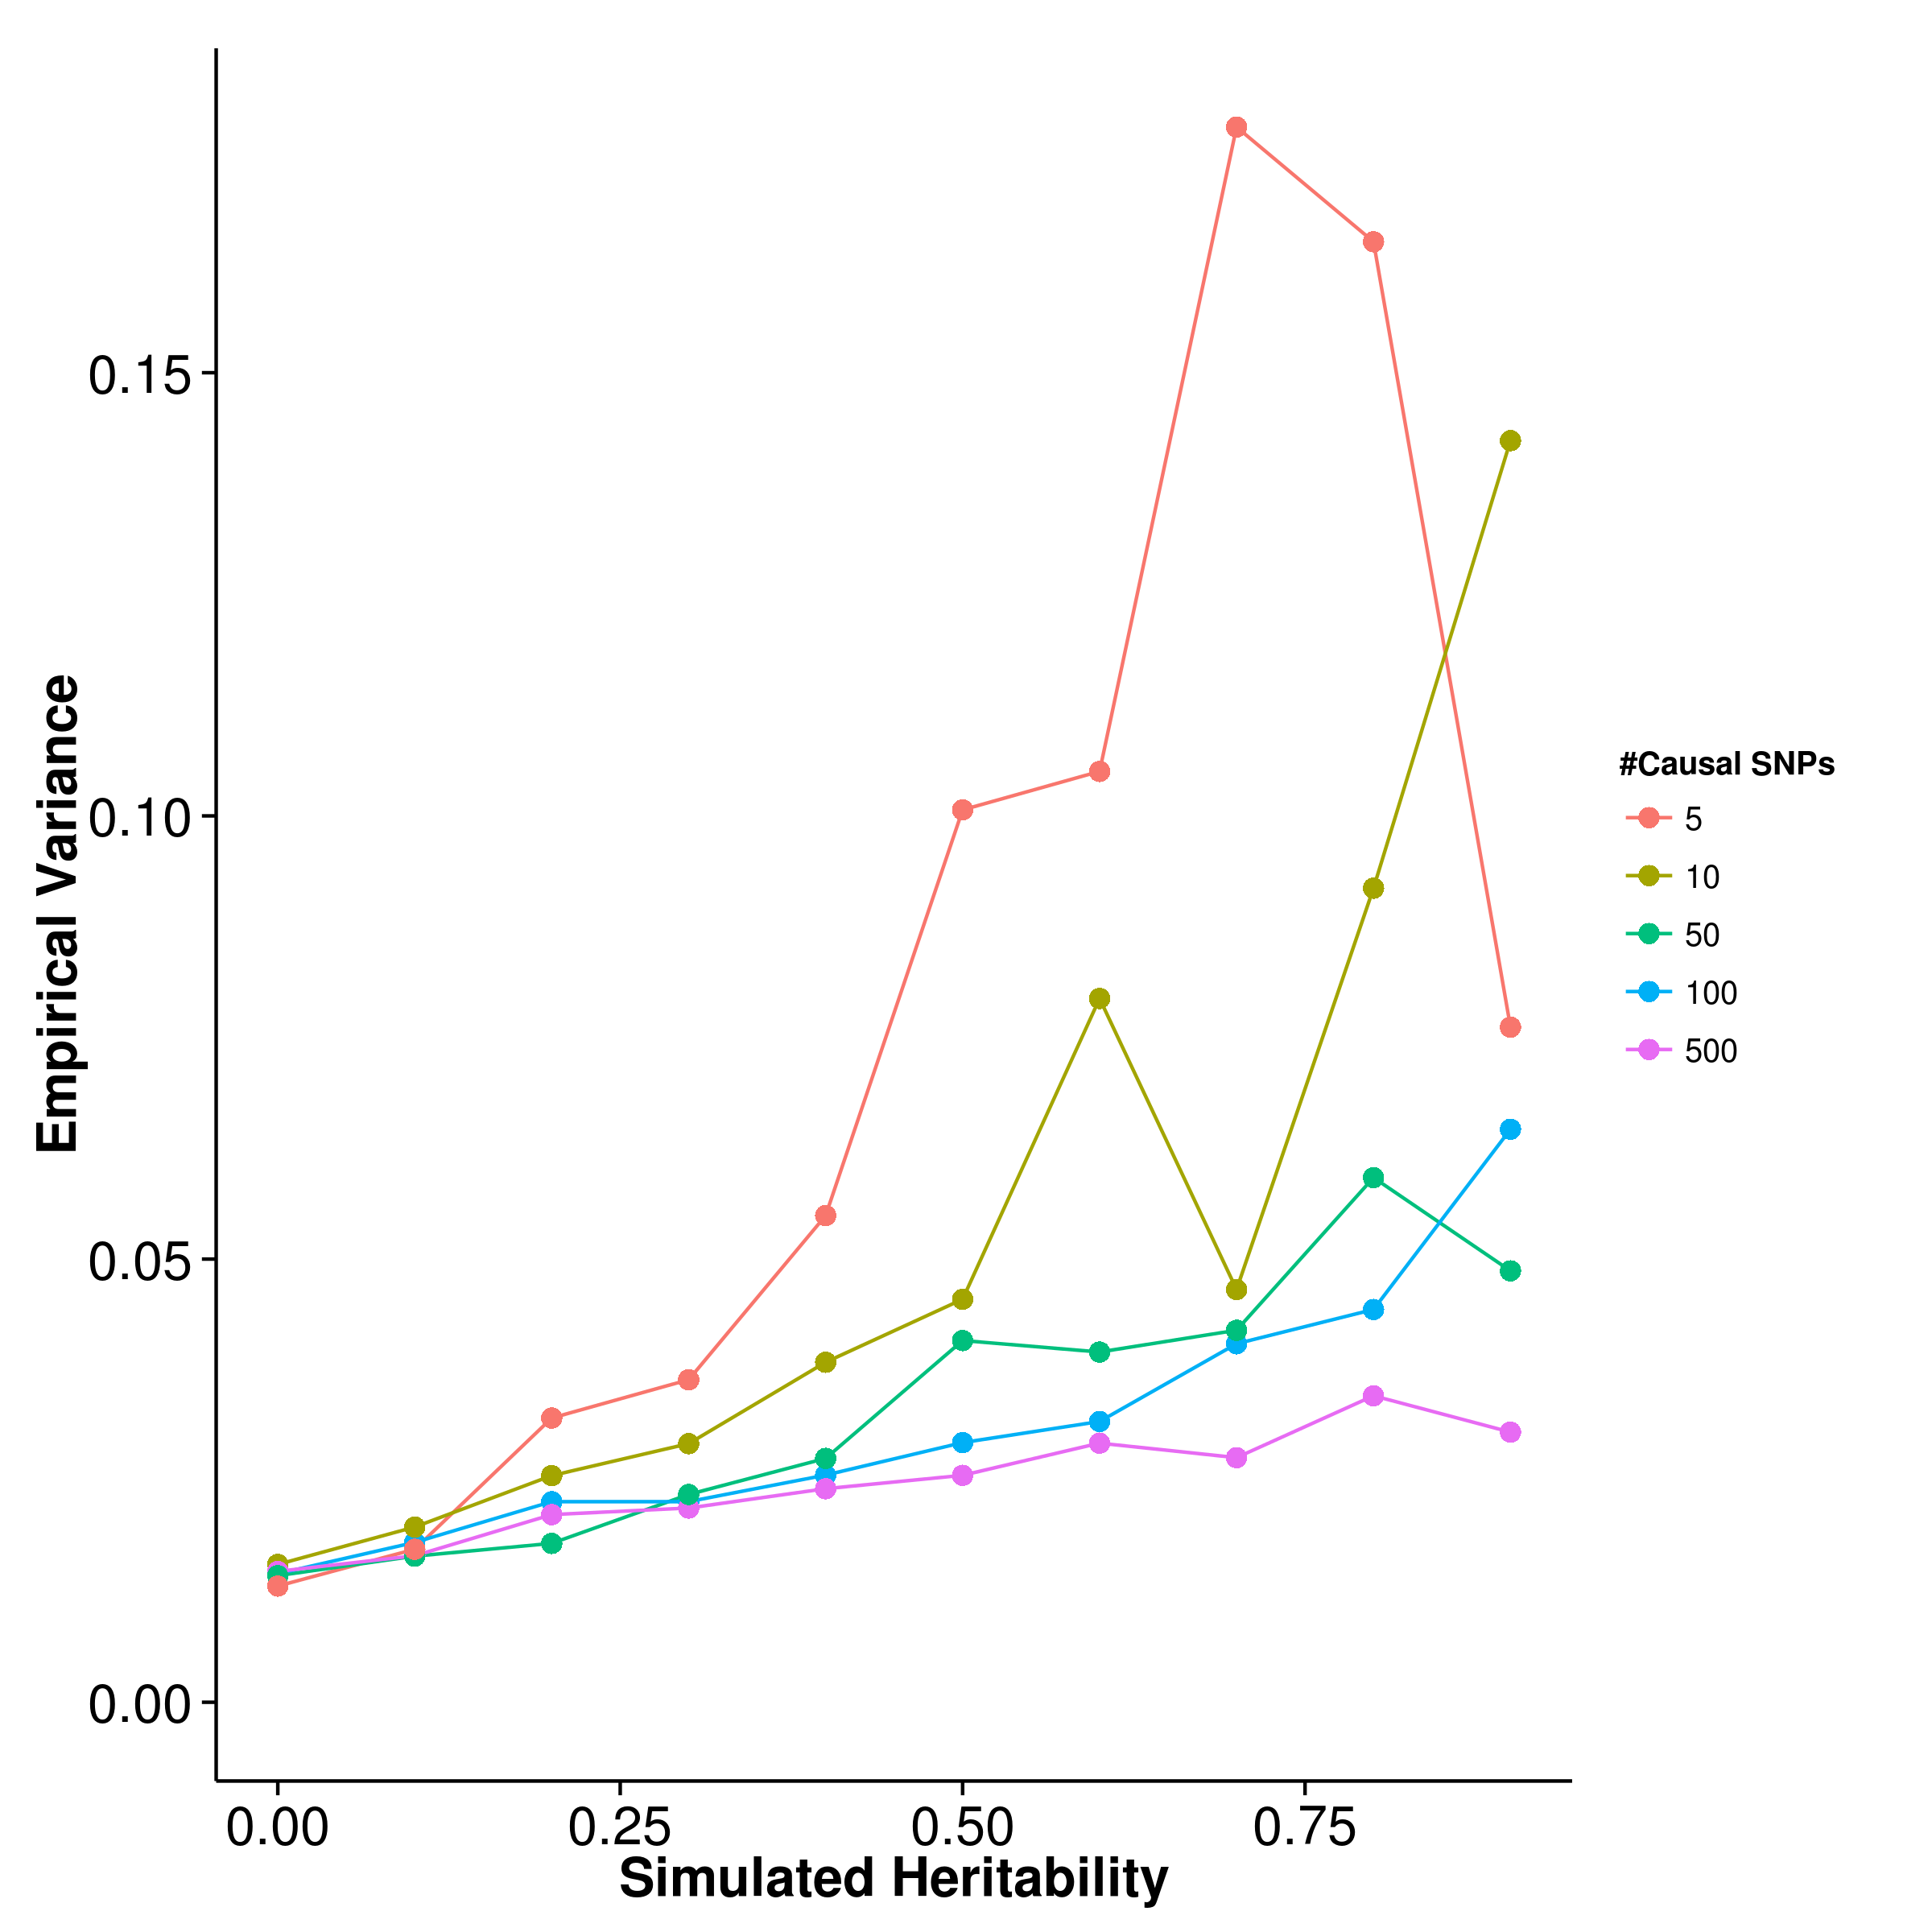
\includegraphics{figure/he_summary/random/ldscIn_Qt_Rand_sd.png}}
		\label{fig:ldscInQtRandVar}
	}
	\caption[Variance of Quantitative Trait Simulation Results]
	{Variance of results from quantitative trait simulation with random effect size simulation.
		Under the polygenic conditions, \gls{gcta} has the smallest variance, follow by \gls{ldsc}. 
		However, it was observed when the number of causal \glspl{SNP} decreases, the variance of the estimation increases for all algorithm, with variance of the \gls{shrek} estimate being the least affected.
		In fact, under oligogenic conditions, \gls{shrek} has a lower empirical variance when compared to \gls{ldsc}.
	} 
	\label{fig:QtRandVar}
\end{figure}
%Variance estimate
\begin{figure}
	\centering
	\subfloat[SHREK]{
		\scalebox{.4}{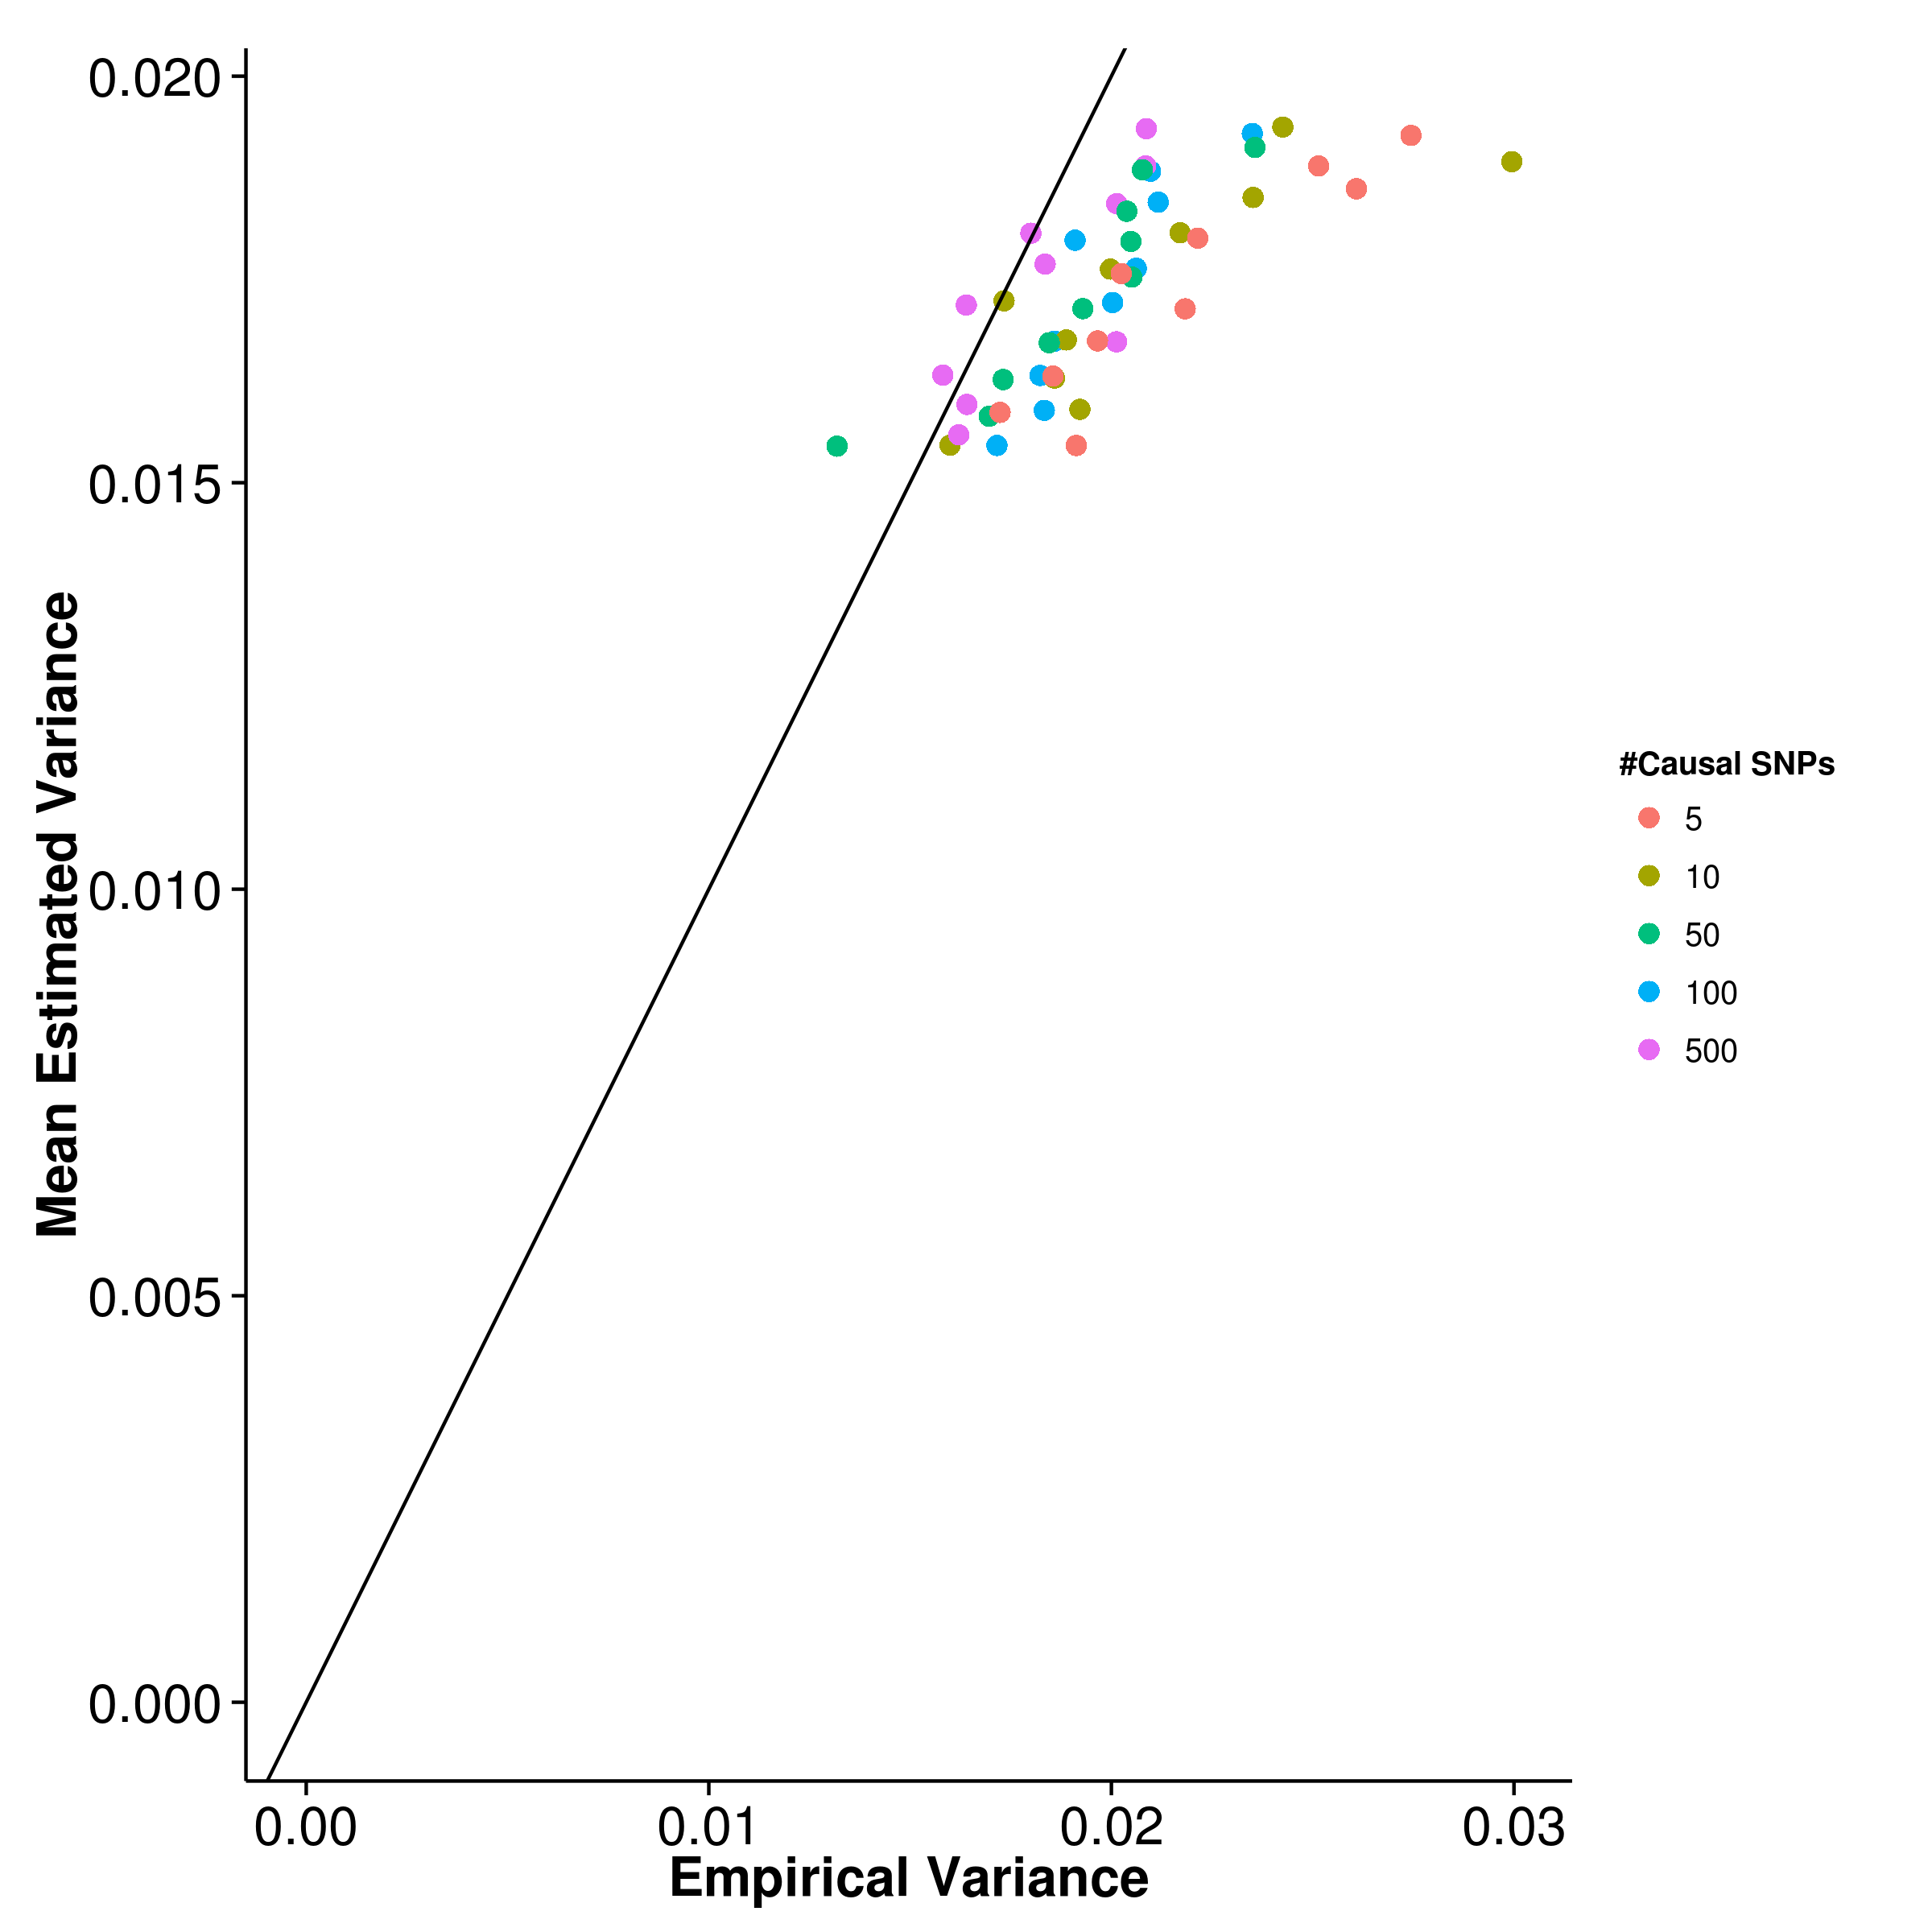
\includegraphics{figure/he_summary/random/shrek_Qt_Rand_sdCom.png}}
		\label{fig:shrekQtRandVarCom}
	}
	\subfloat[GCTA]{
		\scalebox{.4}{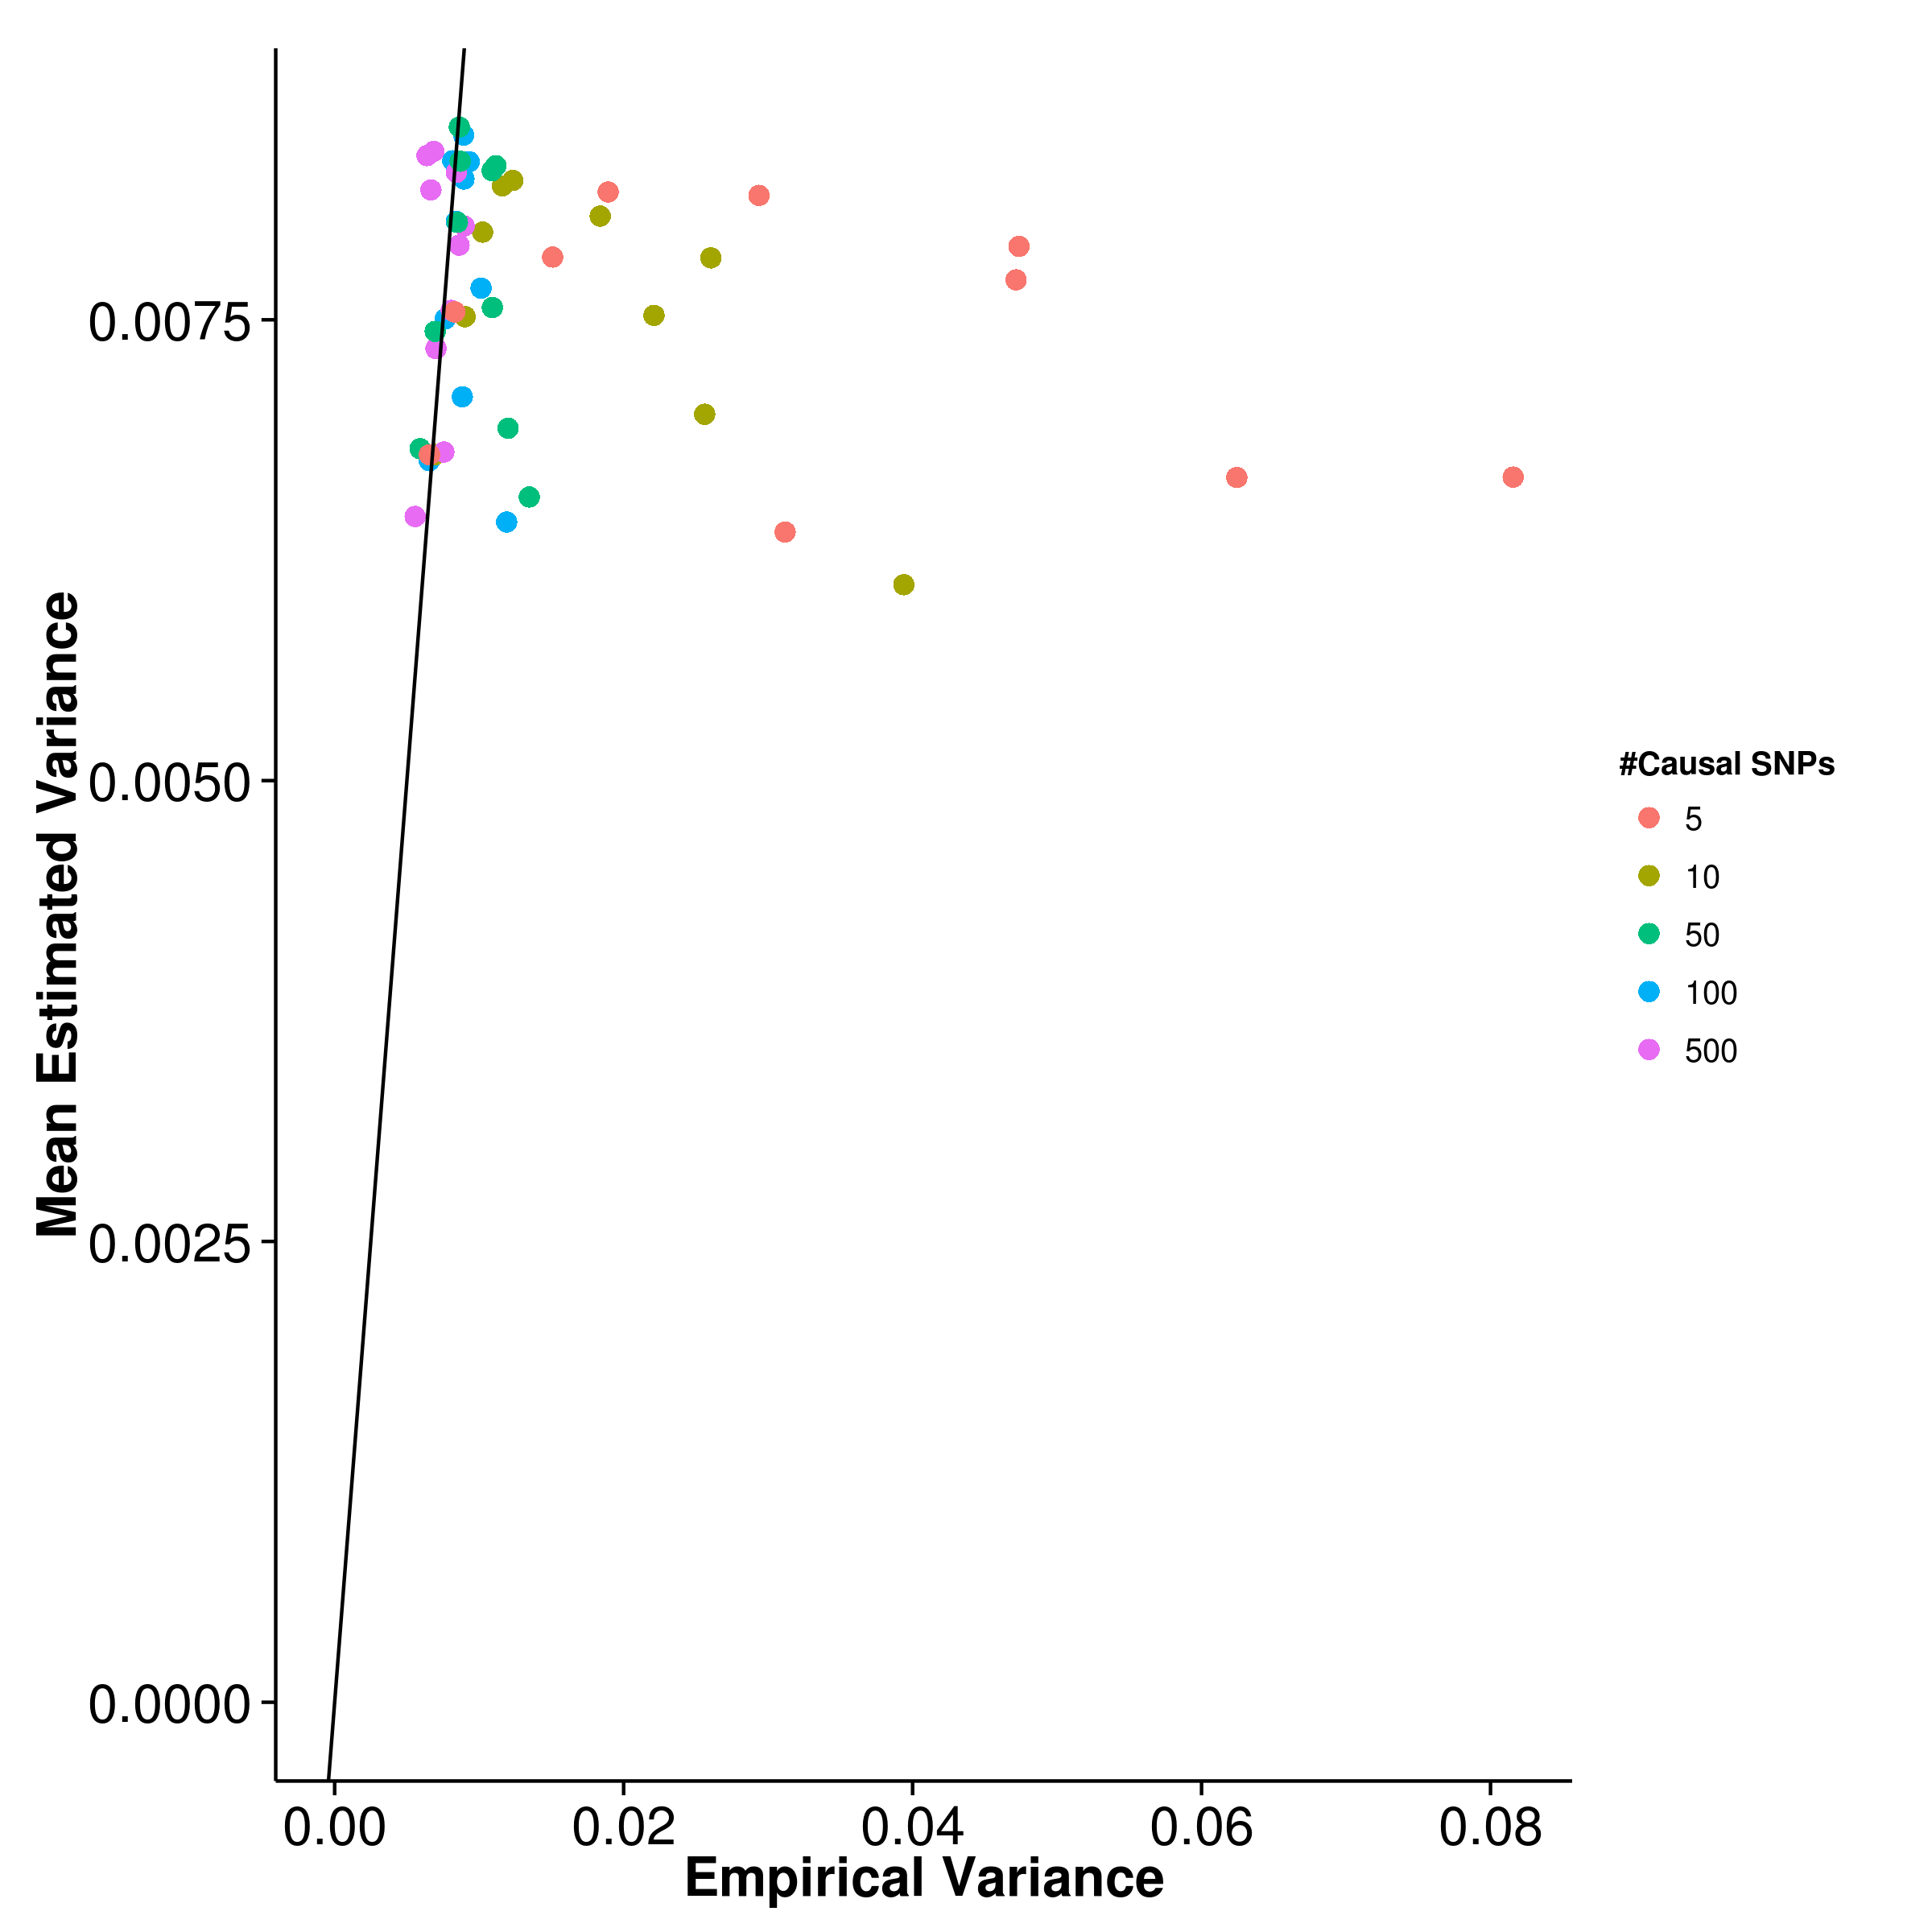
\includegraphics{figure/he_summary/random/gcta_Qt_Rand_sdCom.png}}
		\label{fig:gctaQtRandVarCom}
	}\\
	\subfloat[LDSC with fix intercept]{
		\scalebox{.4}{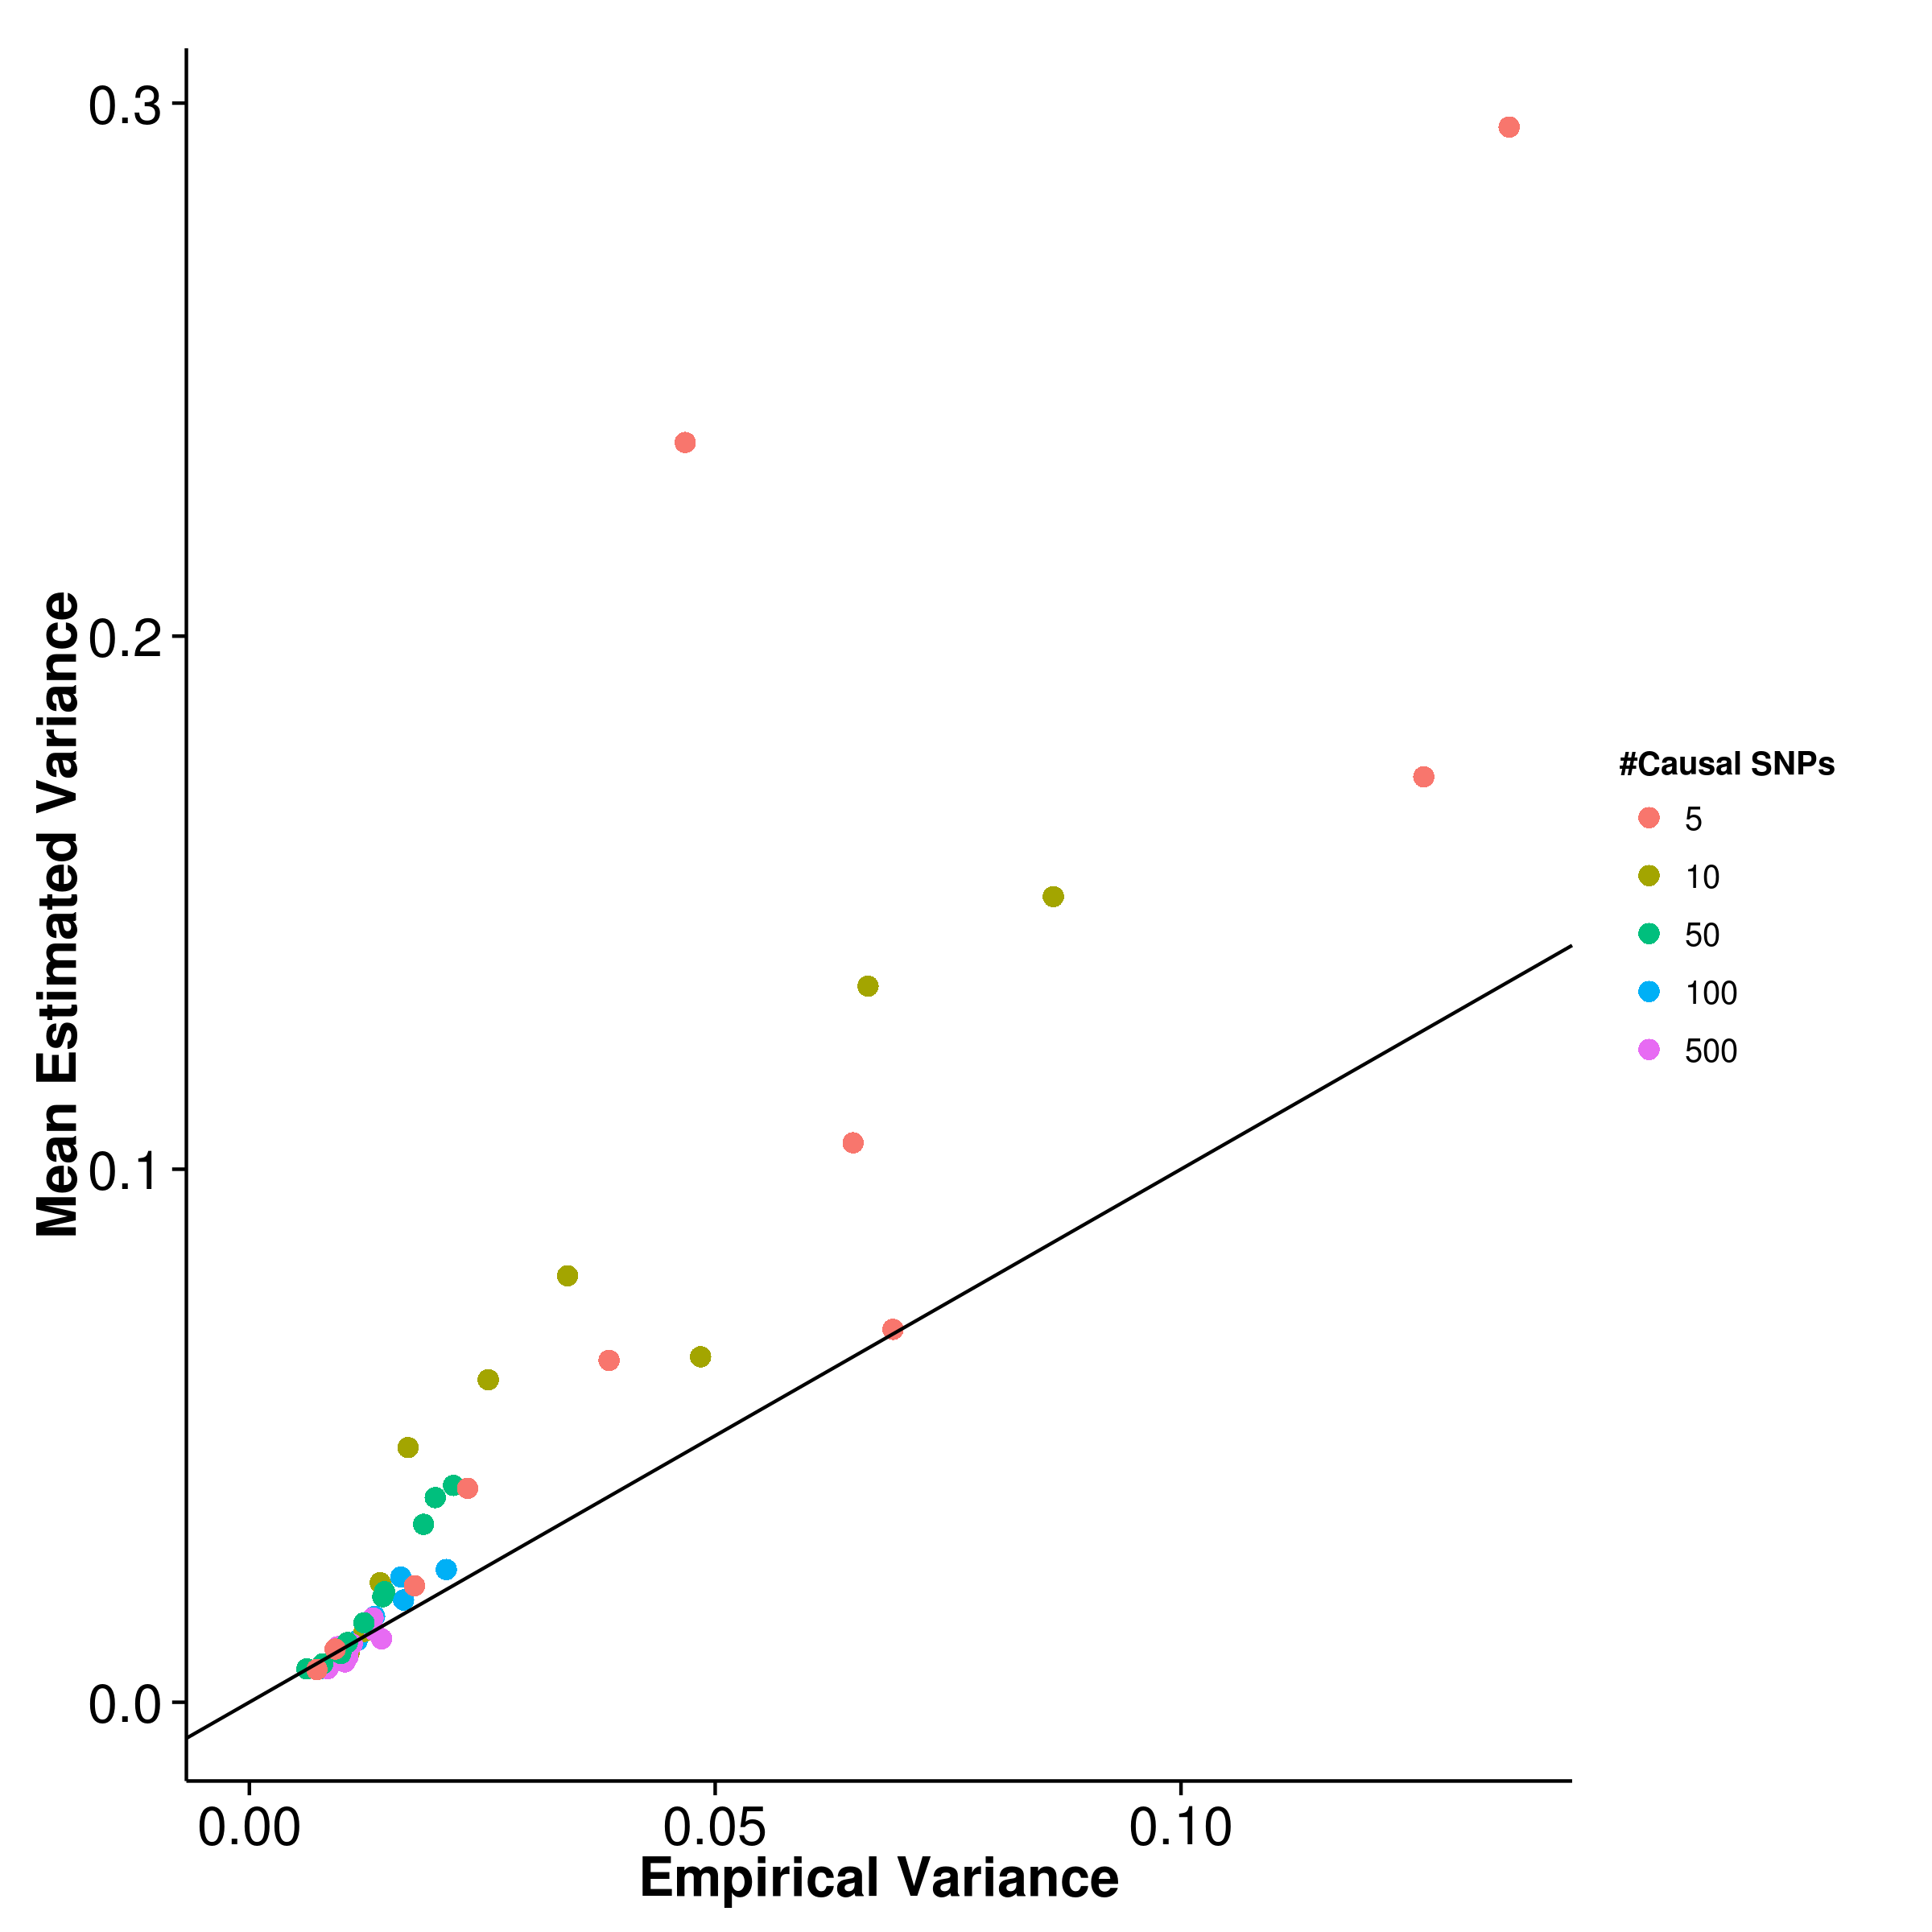
\includegraphics{figure/he_summary/random/ldsc_Qt_Rand_sdCom.png}}
		\label{fig:ldscQtRandVarCom}
	}
	\subfloat[LDSC with intercept estimation]{
		
		\scalebox{.4}{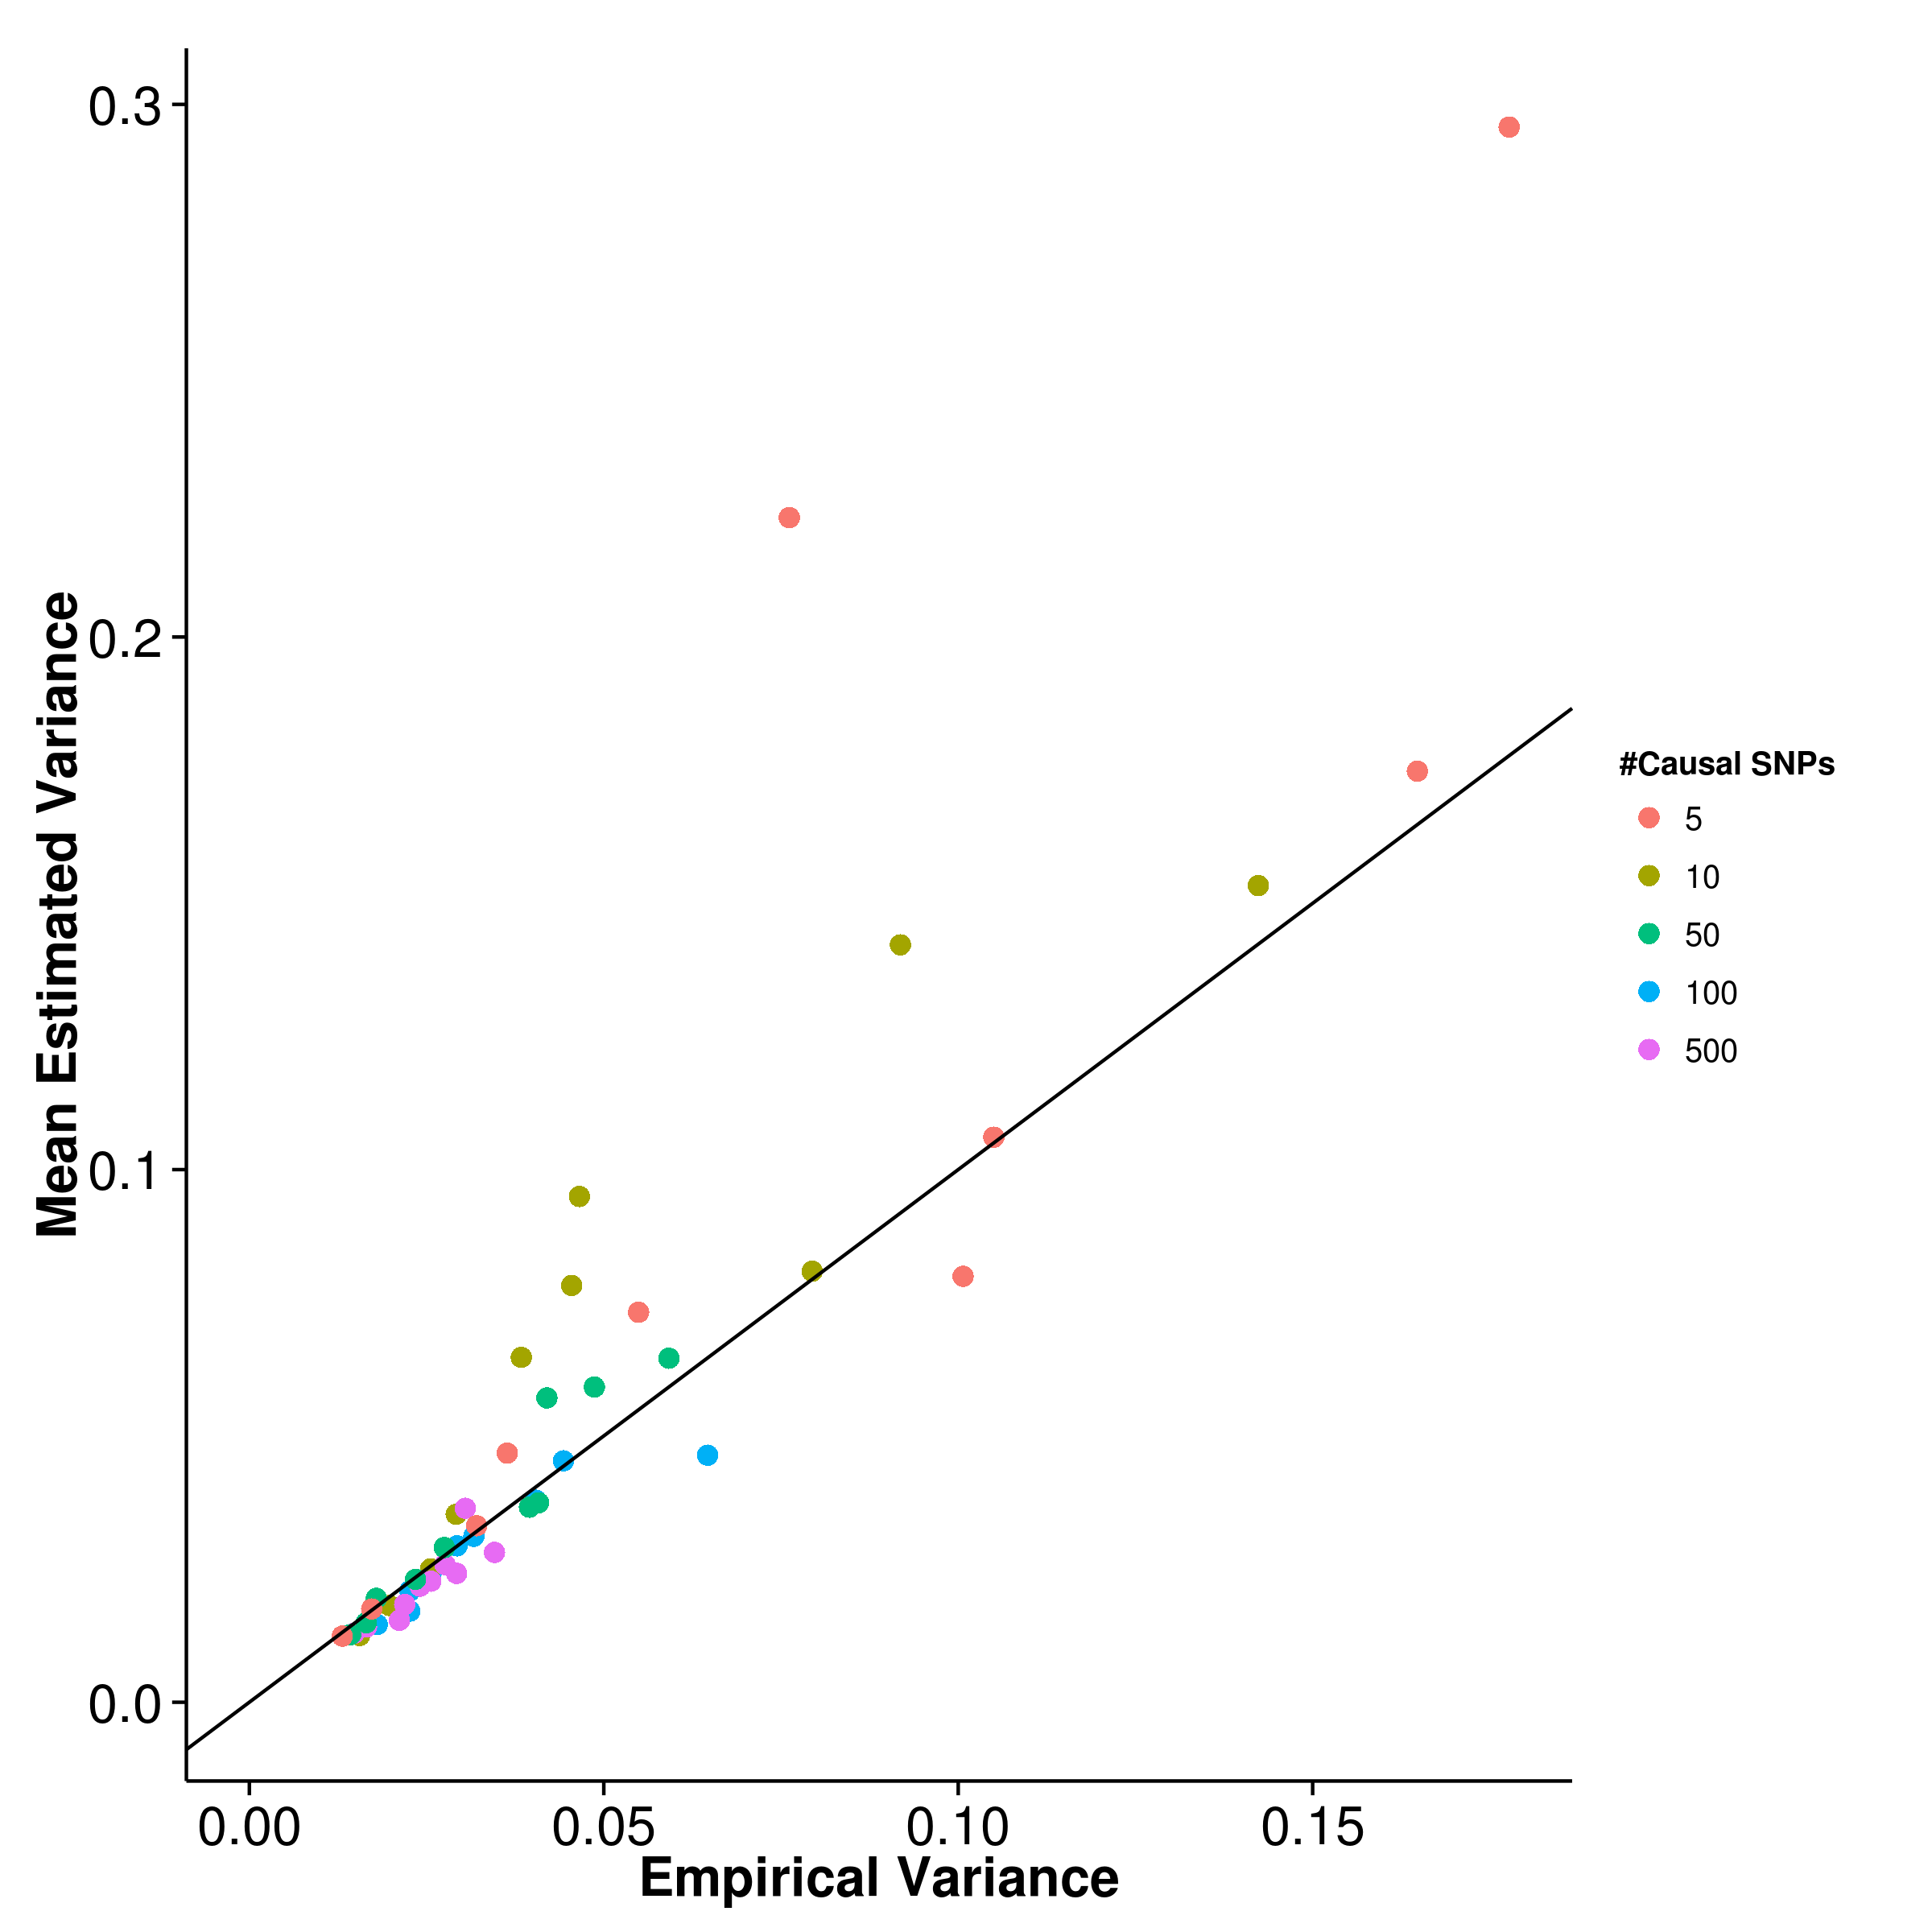
\includegraphics{figure/he_summary/random/ldscIn_Qt_Rand_sdCom.png}}
		\label{fig:ldscInQtRandVarCom}
	}
	\caption[Estimation of Variance in Quantitative Trait Simulation]
	{Estimated variance of results from quantitative trait simulation with random effect size simulation when compared to the empirical variance.
		\gls{gcta} has the best estimate of its empirical variance under the polygenic conditions whereas \gls{shrek} tends to under-estimate its empirical variance.
		On the other hand, \gls{ldsc} tends to over-estimate the variance especially when the number of causal \glspl{SNP} is small.
	} 
	\label{fig:QtRandVarCom}
\end{figure}
By varying the number of causal \glspl{SNP} and the heritability of the trait, performance of \gls{ldsc}, \gls{shrek} and \gls{gcta} can be investigated.

First, when comparing the mean estimates to the simulated heritability, a small upward bias is observed in the estimates from \gls{shrek} (\cref{fig:shrekQtRandMean}).
On the other hand, estimates from \gls{gcta} are moderately biased downward (\cref{fig:gctaQtRandMean}), similar to the estimates from \gls{ldsc} with intercept estimation (\cref{fig:ldscInQtRandMean}), but with a smaller variability.
When the intercept was fixed, \gls{ldsc} can accurately estimate the \gls{SNP} heritability where an upward bias can only be observed when the number of \glspl{SNP} is small.

Second, the empirical variance of the estimates is another important indicator of the performance of the algorithms.
It is clear that empirical variance of the estimates from \gls{ldsc} are sensitive to the number of  causal \glspl{SNP} (\cref{fig:ldscQtRandVar,fig:ldscInQtRandVar}).
When the number of causal \glspl{SNP} decreases, the variance of the estimates increases, as reported by \citet{Bulik-Sullivan2015}.
Moreover, consistent with the results from \citet{Bulik-Sullivan2015}, the intercept estimation increases the variance of the estimates from \gls{ldsc}.
Similarly, the variance of the estimates form \gls{gcta} also increases when the number of causal \glspl{SNP} decreases (\cref{fig:gctaQtRandVar}), despite it has the lowest variance in its estimates.
On the other hand, estimates from \gls{shrek} are relatively insensitive to the number of causal \glspl{SNP}.

\begin{table}
	\centering
	\begin{tabular}{rrrrr}
		\toprule
		Number of Causal SNPs&	SHREK&	LDSC&	LDSC-In&	GCTA \\
		\midrule
		5	&	0.0235	&	0.0576	&	0.0828	&	0.0365\\
		10	&	0.0231	&	0.0343	&	0.0555	&	0.0189\\
		50	&	0.0196	&	0.0157	&	0.0494	&	0.0114\\
		100	&	0.0210	&	0.0129	&	0.0363	&	0.00961\\
		500	&	0.0205	&	0.0115	&	0.0308	&	0.00887\\
		\bottomrule
	\end{tabular}
	\caption[MSE of Quantitative Trait Simulation with Random Effect Size]{
		\Gls{mse} of quantitative trait simulation with random effect size.
		Of all the algorithms, \gls{gcta} has the lowest \gls{mse} except when there is only 5 causal \glspl{SNP}.
		When comparing the performance of \gls{shrek} and \gls{ldsc} with fixed intercept, the performance of \gls{shrek} is better under the oligogenic condition whereas \gls{ldsc} with fixed intercept excels under the polygenic condition. 
		On the other hand, when intercept estimation were performed, the \gls{mse} of \gls{ldsc} increases, mainly due to the increased \gls{se}. 
		Therefore \gls{shrek} outperforms \gls{ldsc} with intercept estimation when there are minimal confounding variables.
	}
	\label{tab:mseQtRandom}
\end{table}
Finally, it is important for the algorithms to be able to estimate the standard error of its estimates. 
Therefore, the estimated variance is compared with the empirical variance of the estimates.
It is observed that with a large number of causal \glspl{SNP}, \gls{gcta} can accurately estimates its variance (\cref{fig:gctaQtRandVarCom}).
However, when the number of causal \glspl{SNP} is small, \gls{gcta} underestimates the variance of its estimates. 
On the other hand, \gls{shrek} consistently underestimate the variance of its estimates (\cref{fig:shrekQtRandVarCom}).
But when compared to \gls{ldsc}, the magnitude of bias of the variance estimated from \gls{shrek} is much smaller.
\gls{ldsc} tends to overestimate its variance (\cref{fig:ldscQtRandVarCom,fig:ldscInQtRandVarCom}), and only when the intercept estimation was performed can \gls{ldsc} has a better estimates of the variance when the number of causal \glspl{SNP} is large. 
Although the bias of the variance estimated from \gls{shrek} is much smaller than \gls{ldsc}, its variance estimate tends to be under-conservative which might misleading. 
Further development might be required for \gls{shrek} to provide a better estimate of standard error.

Taking into account of the bias and variance of the estimates, \gls{gcta} has the best overall performance.
On the other hand, when the number of causal \glspl{SNP} is small, \gls{shrek} has a better performance when compared to \gls{ldsc}, whereas \gls{ldsc} performs better under polygenic condition.
It is also observed that estimates from \gls{shrek} is the least sensitive to changes in the genetic architecture among the algorithms tested (\cref{tab:mseQtRandom}).  

\subsubsection{Quantitative Trait Simulation with Extreme Effect Size}
%Mean
\begin{figure}
	\centering
	\subfloat[SHREK]{
		\scalebox{.4}{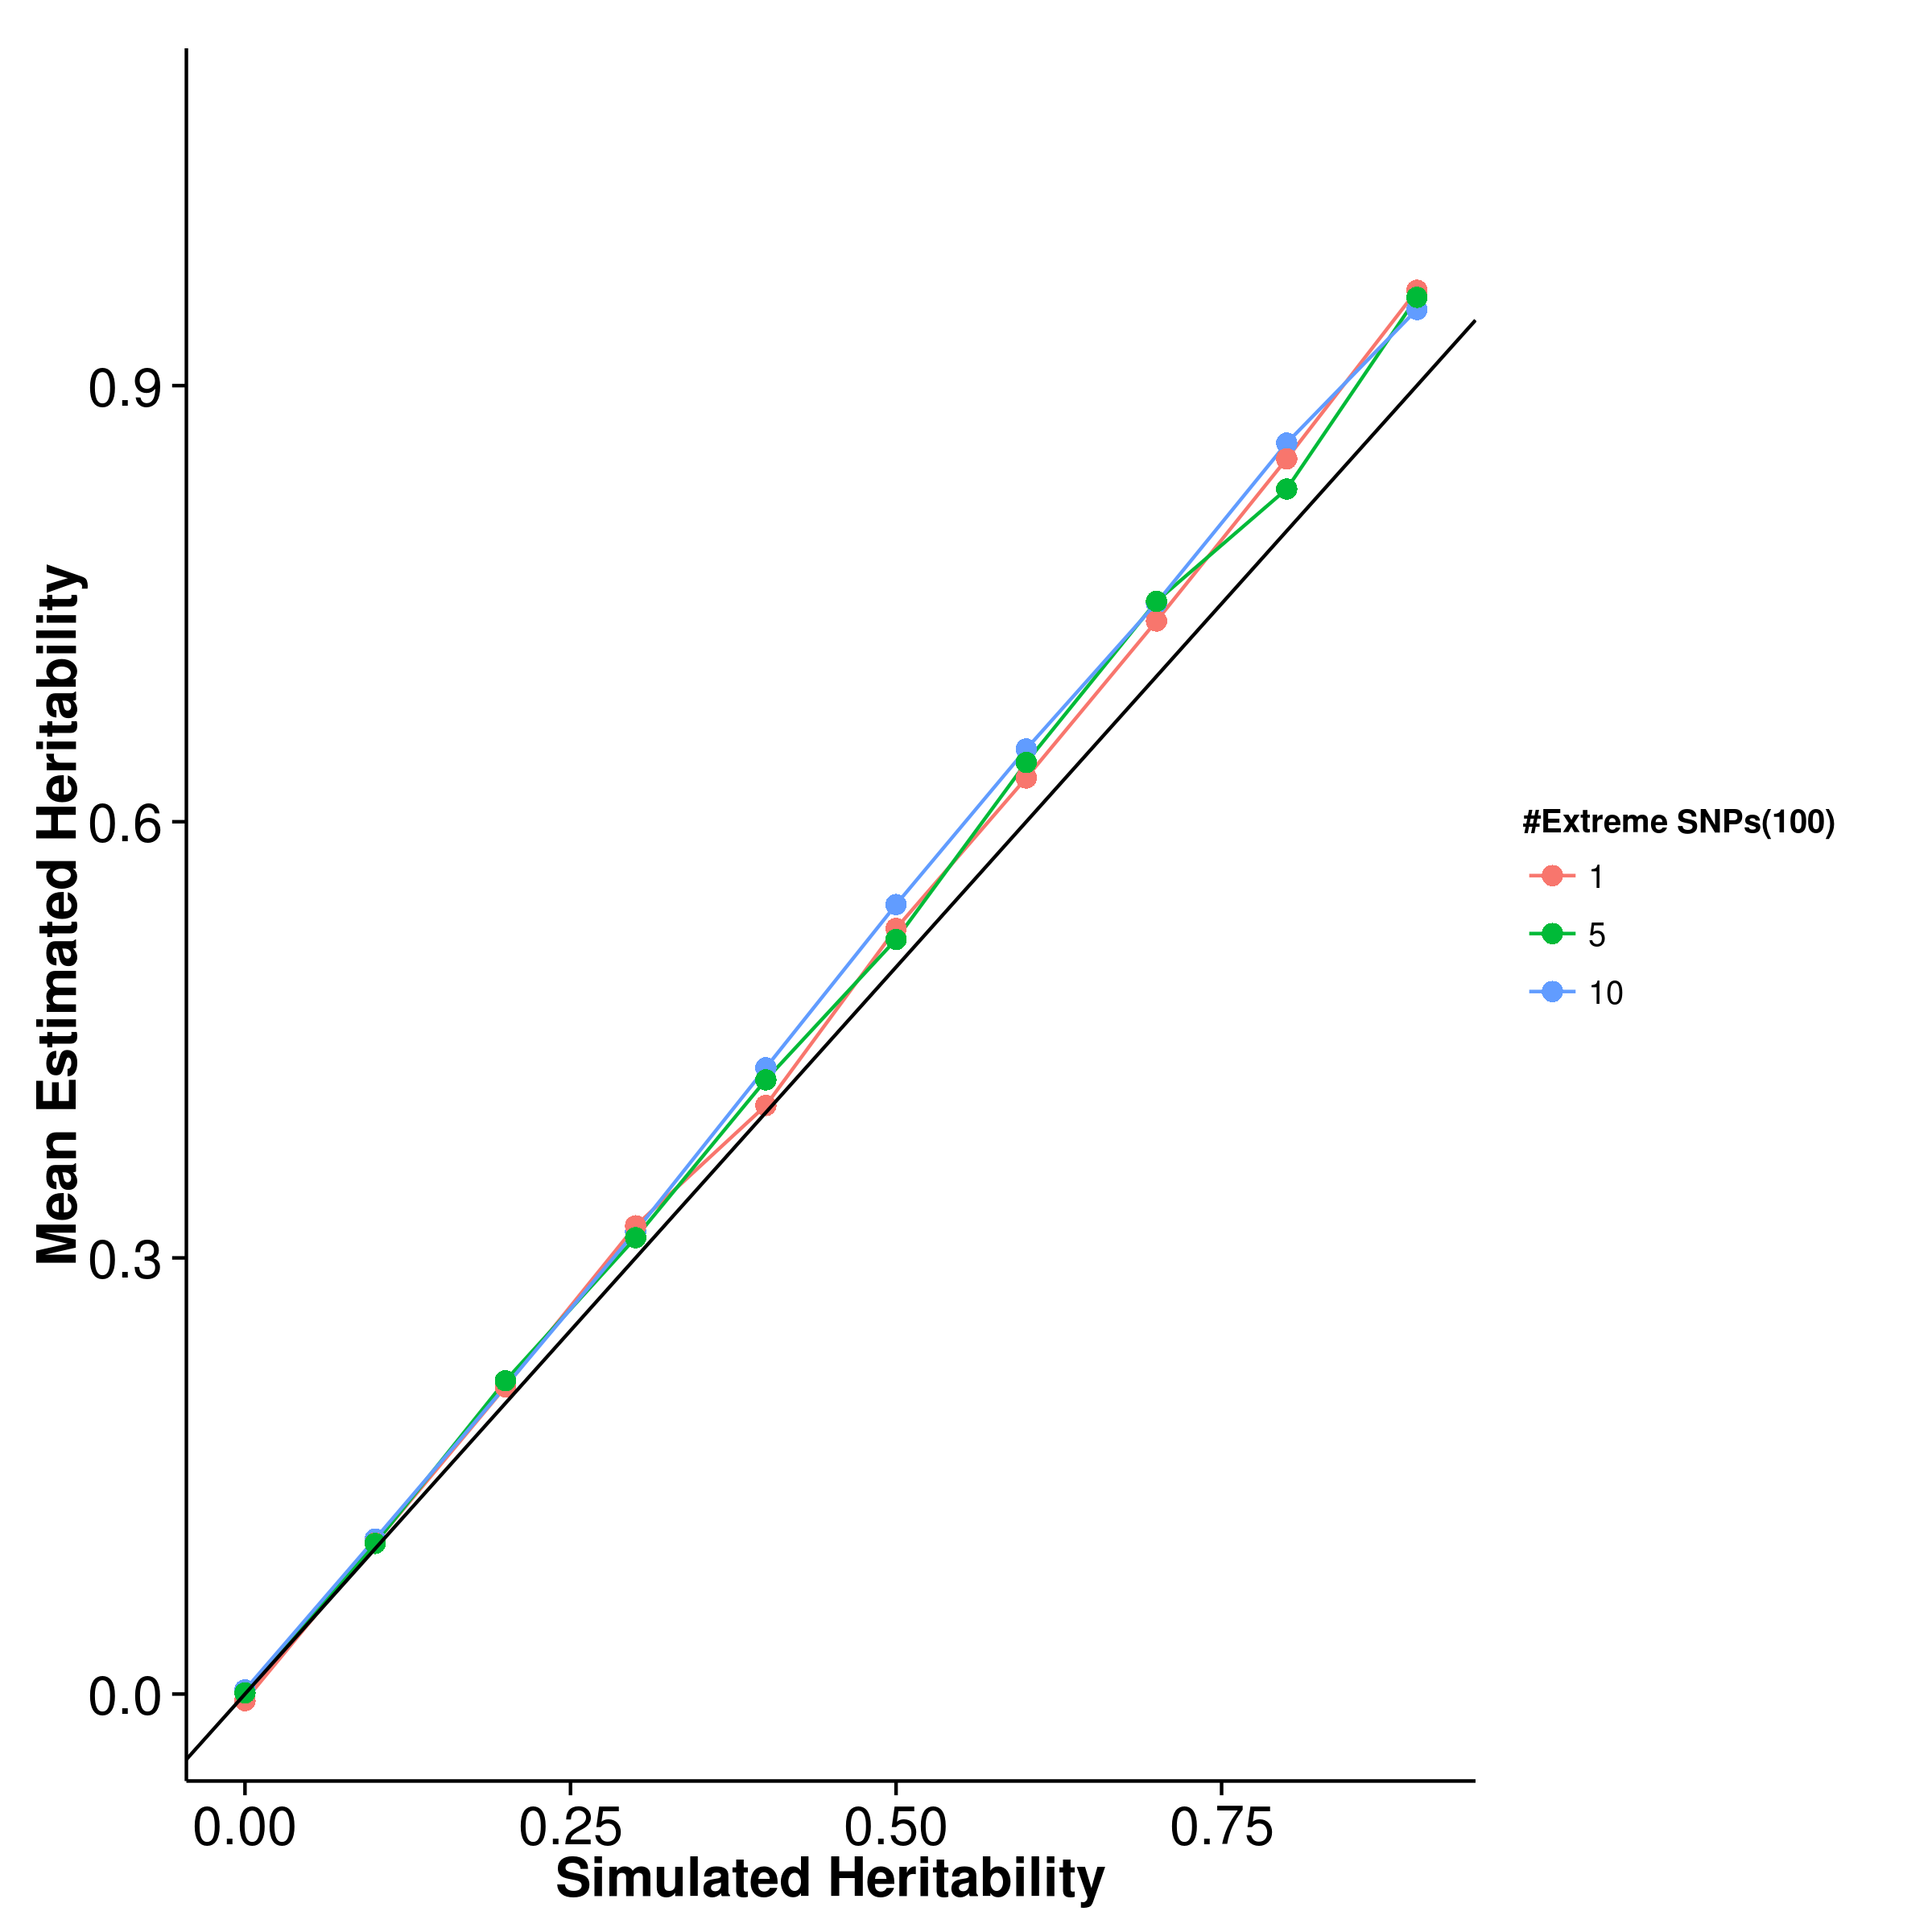
\includegraphics{figure/he_summary/extreme_100c/shrek_QtE_Rand_mean.png}}
		\label{fig:shrekQtEx100cMean}
	}
	\subfloat[GCTA]{
		\scalebox{.4}{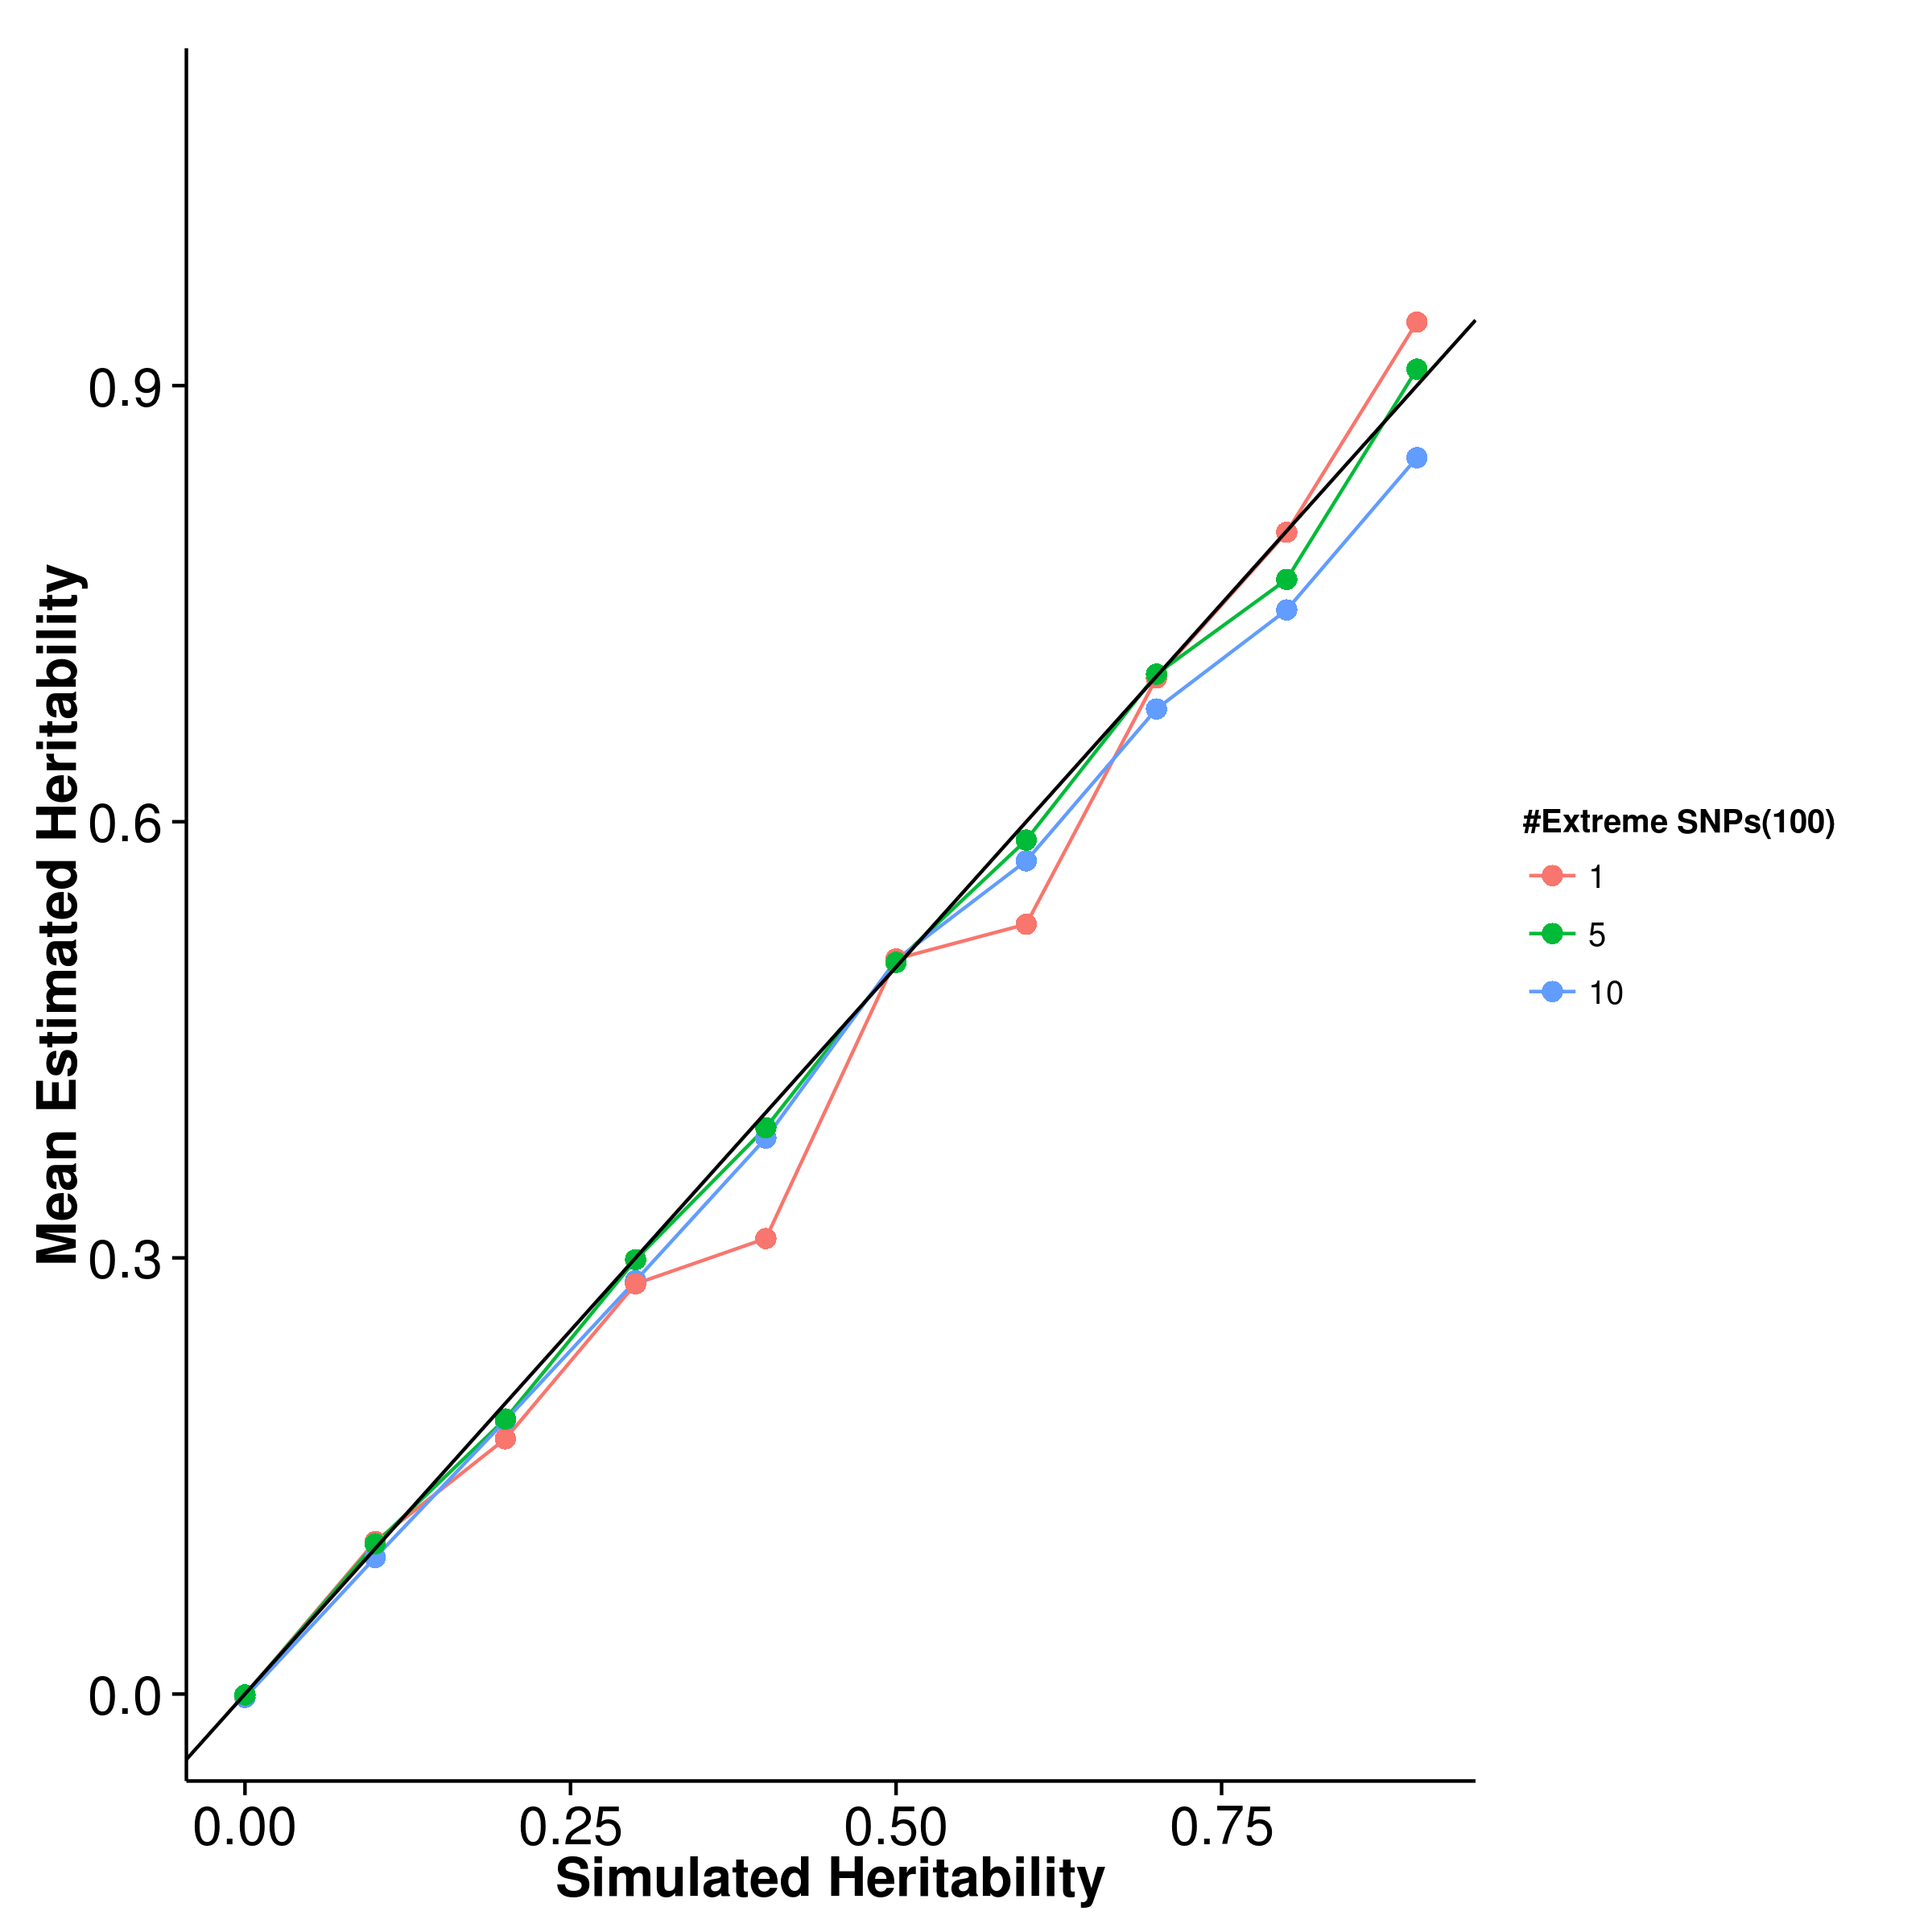
\includegraphics{figure/he_summary/extreme_100c/gcta_QtE_Rand_mean.png}}
		\label{fig:gctaQtEx100cMean}
	}\\
	\subfloat[LDSC with fix intercept]{
		\scalebox{.4}{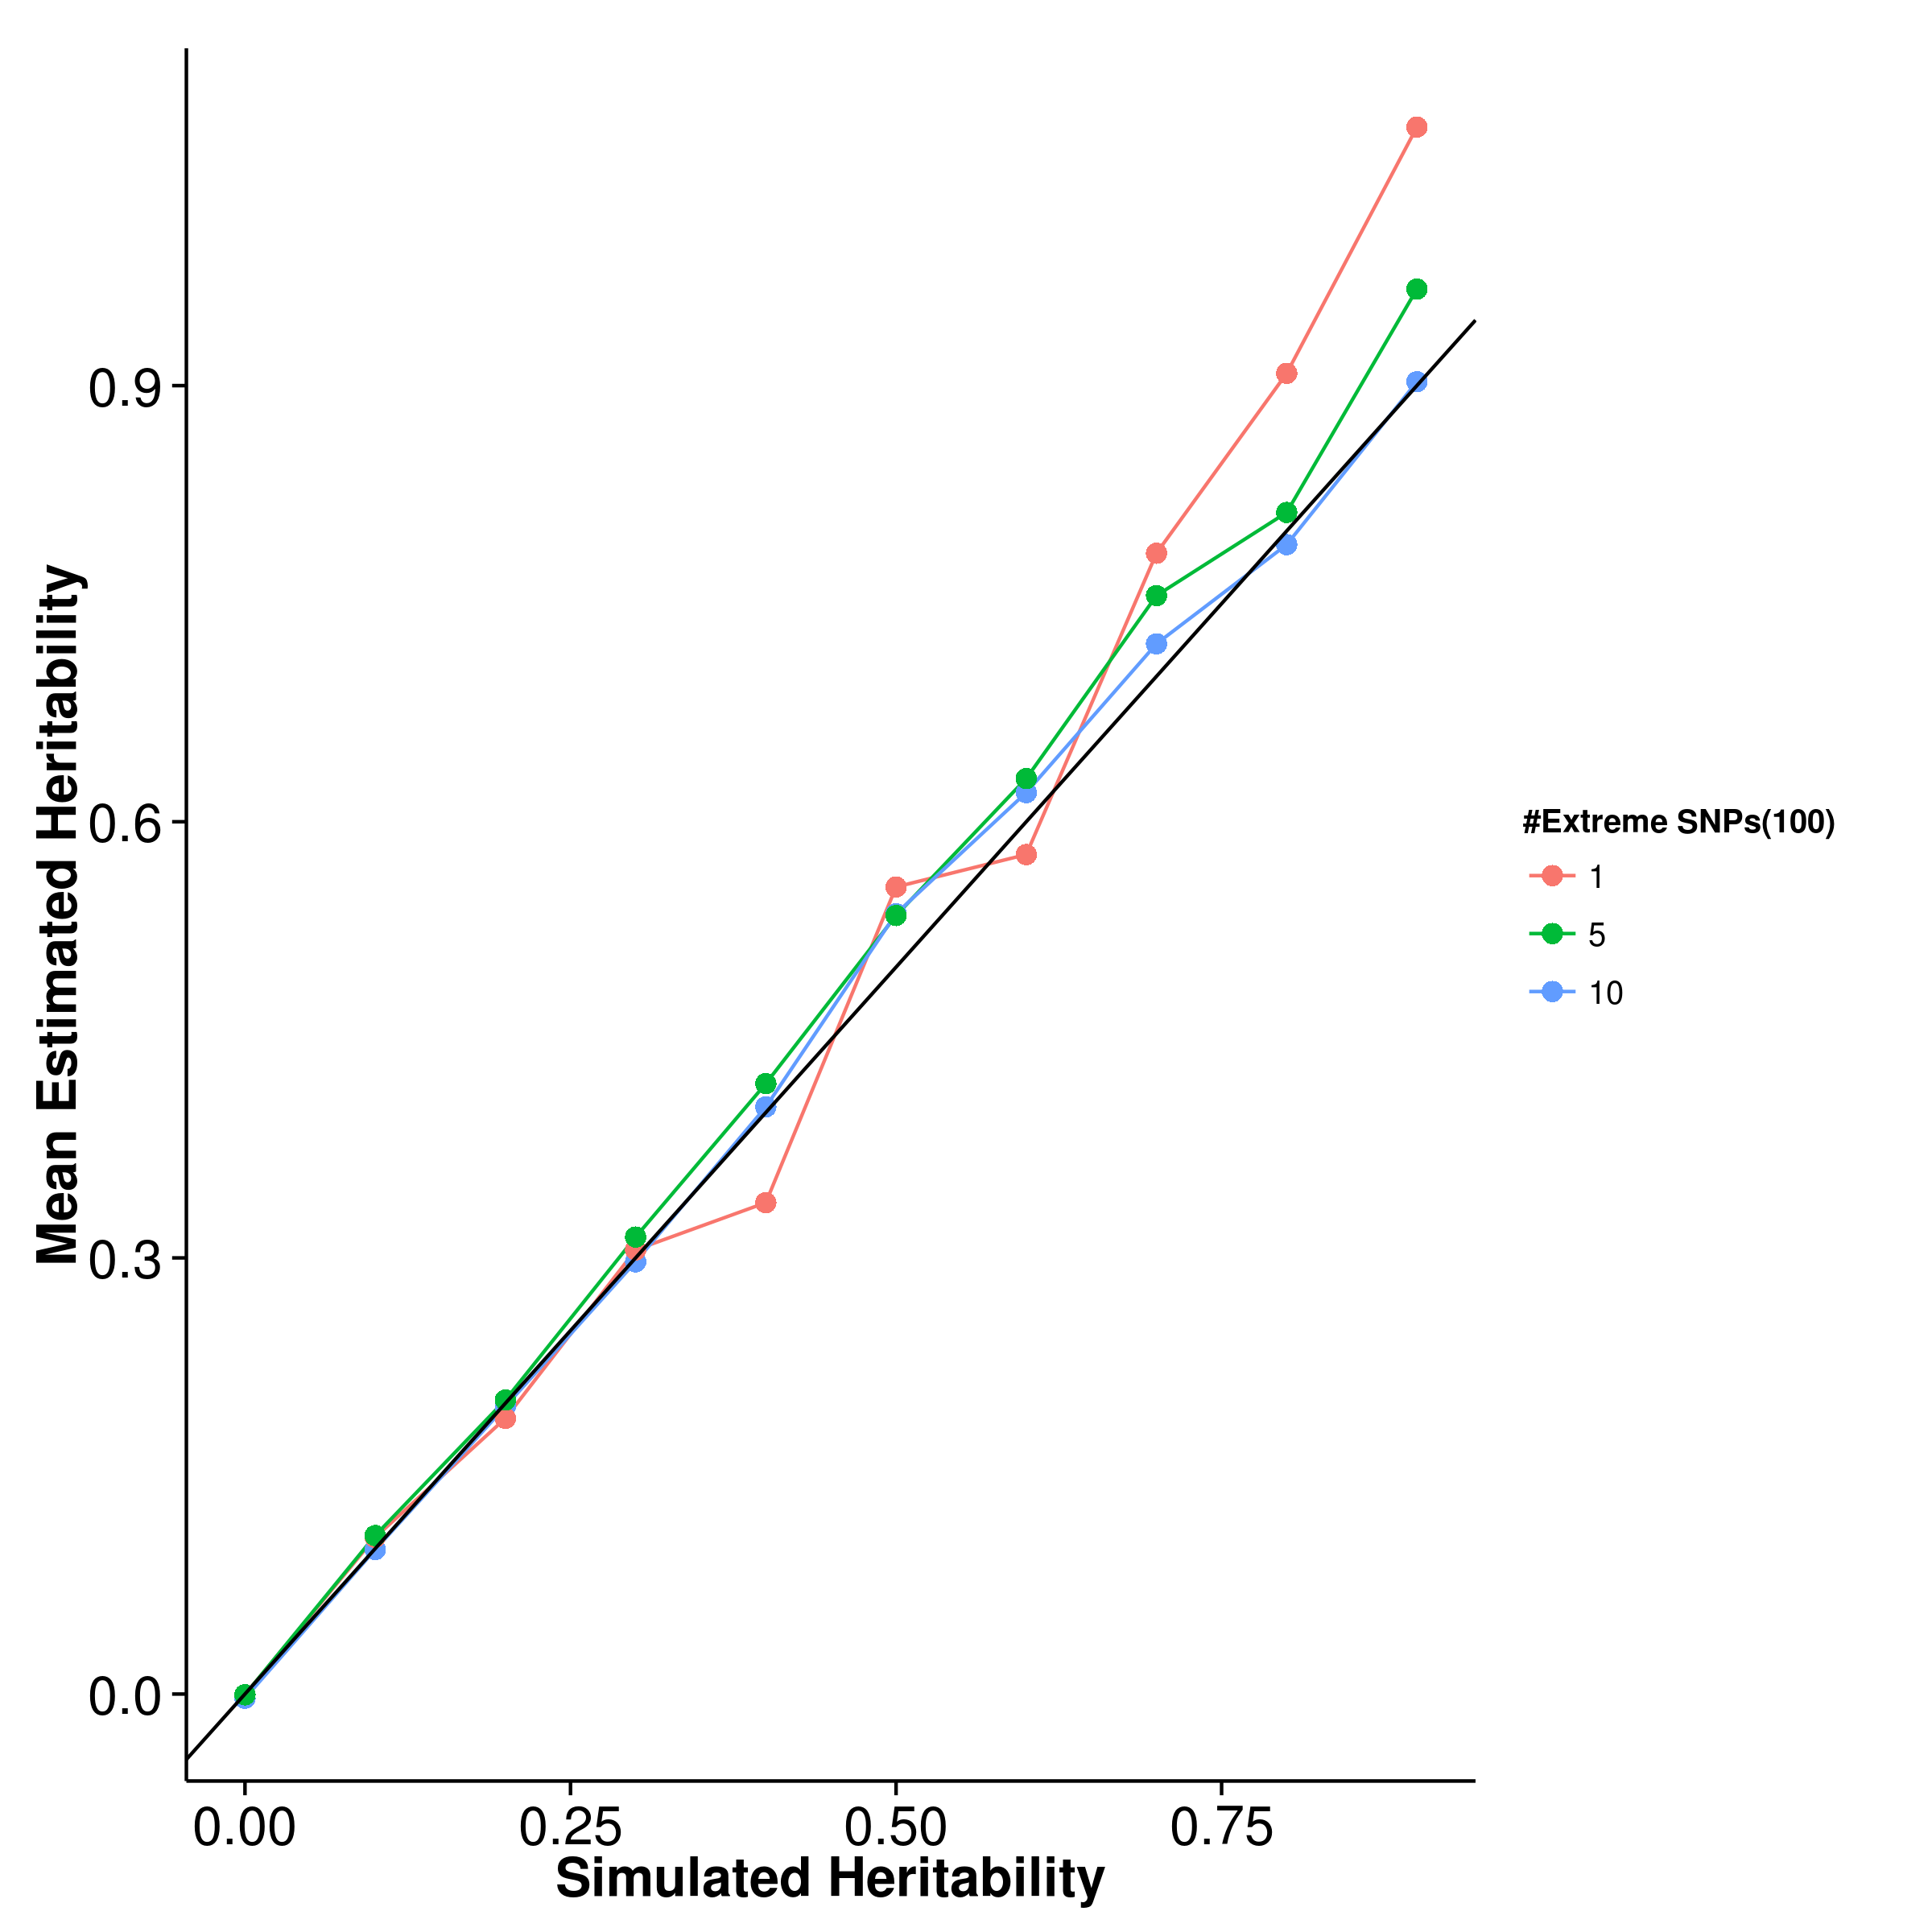
\includegraphics{figure/he_summary/extreme_100c/ldsc_QtE_Rand_mean.png}}
		\label{fig:ldscQtEx100cMean}
	}
	\subfloat[LDSC with intercept estimation]{
		
		\scalebox{.4}{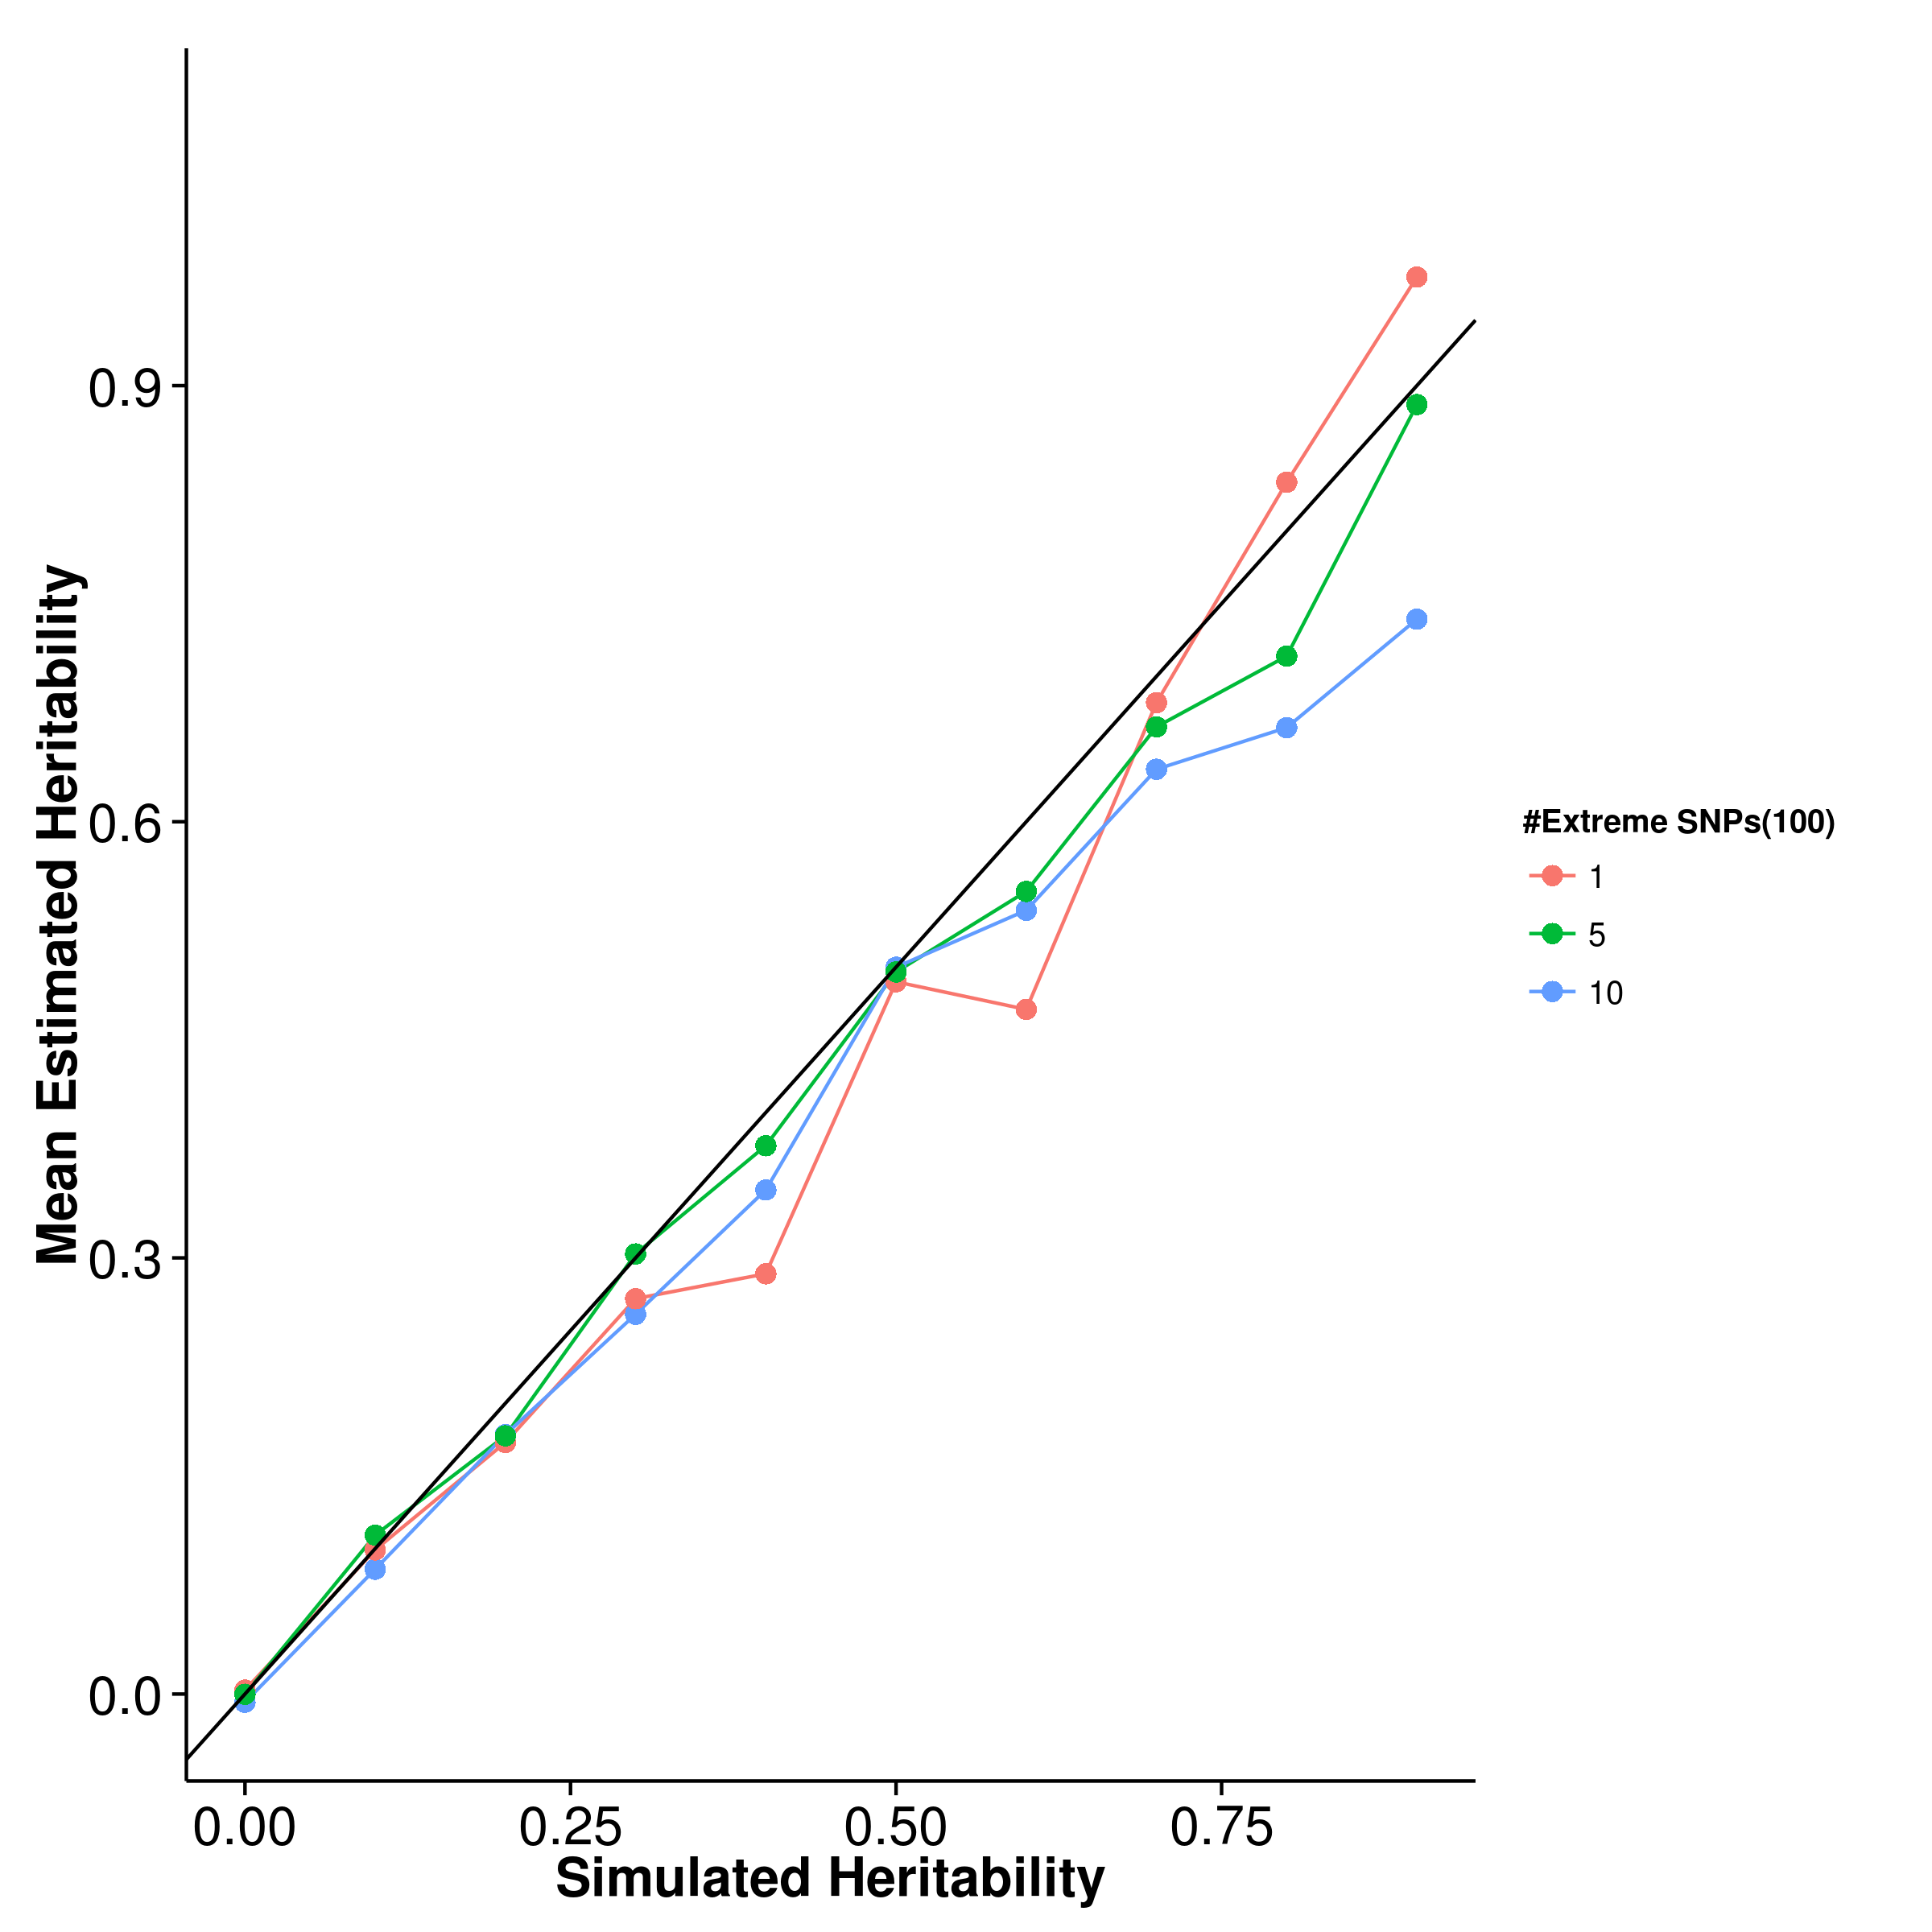
\includegraphics{figure/he_summary/extreme_100c/ldscIn_QtE_Rand_mean.png}}
		\label{fig:ldscInQtEx100cMean}
	}
	\caption[Mean of Extreme Effect Size Simulation Result]
	{Mean of results from quantitative trait simulation with extreme effect size simulation.
		It is observed that the mean estimation of heritability of \gls{shrek} is not affected by the number of \gls{SNP}(s) with large effect but with slight upward bias.
		On the other hand, the mean estimation of \gls{ldsc} and \gls{gcta} seems to fluctuate with respect to the simulated heritability.
	} 
	\label{fig:QtEx100cMean}
\end{figure}
%Empirical Variance
\begin{figure}
	\centering
	\subfloat[SHREK]{
		\scalebox{.4}{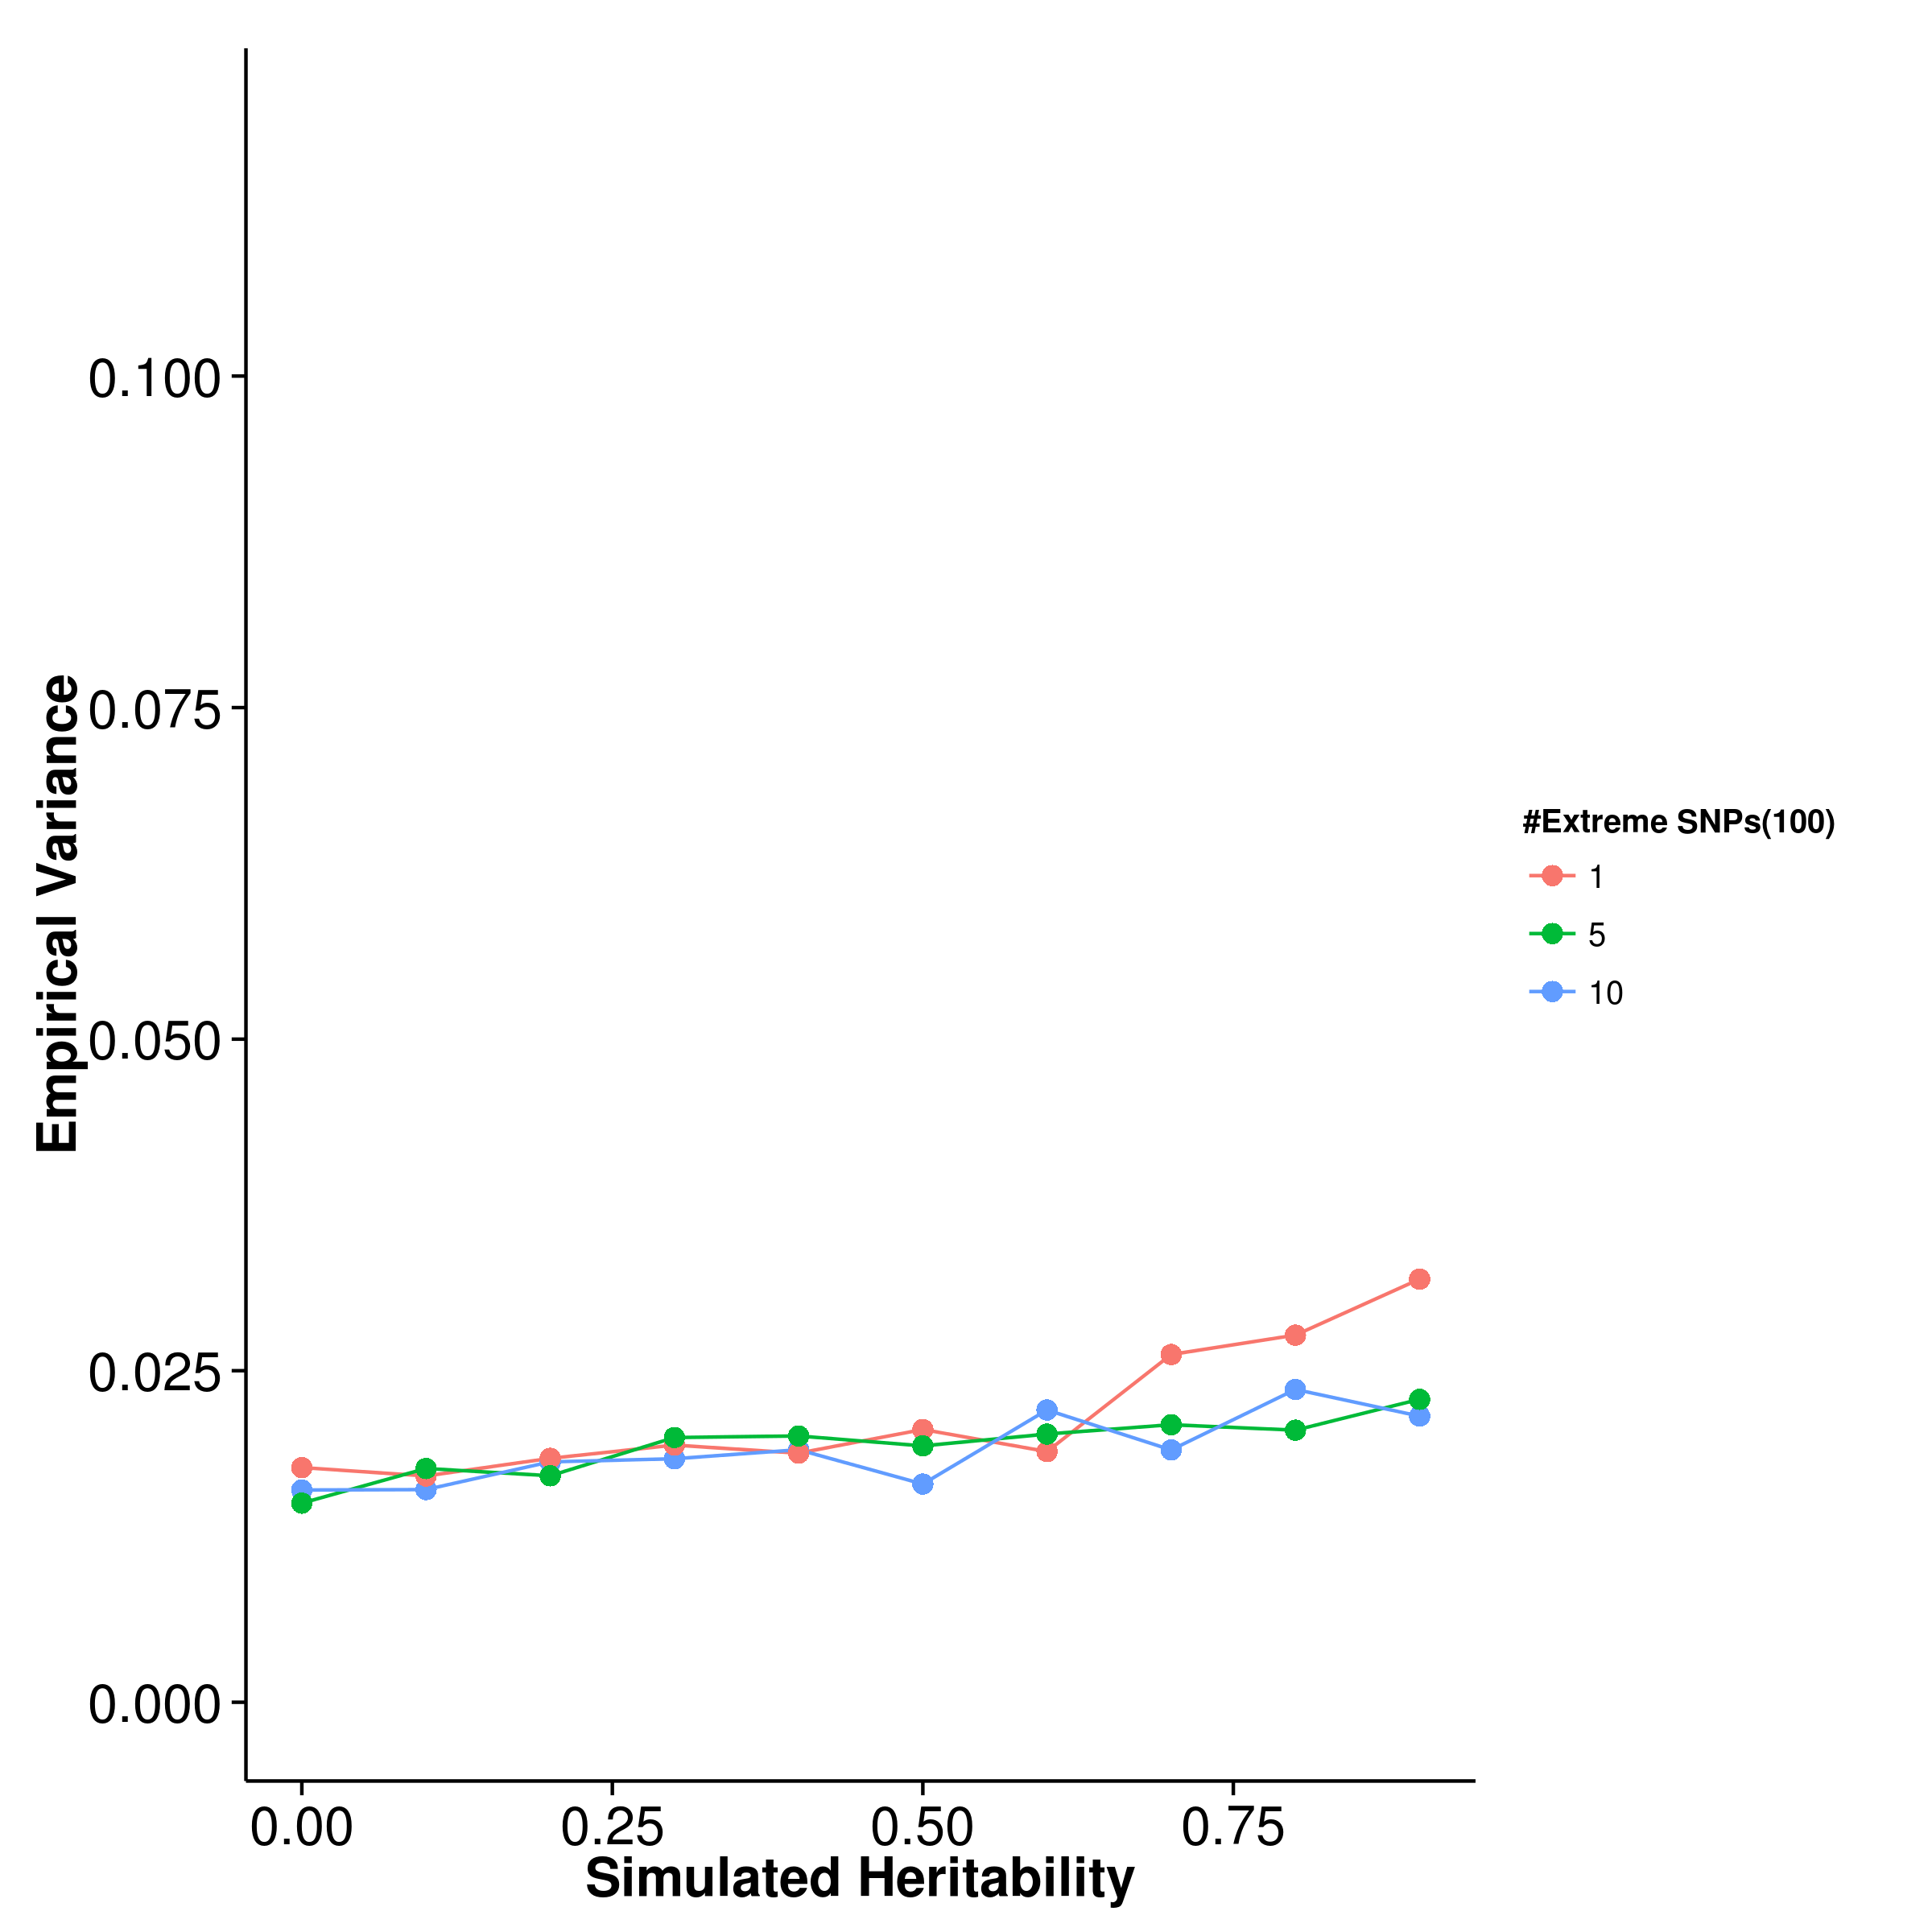
\includegraphics{figure/he_summary/extreme_100c/shrek_QtE_Rand_sd.png}}
		\label{fig:shrekQtEx100cVar}
	}
	\subfloat[GCTA]{
		\scalebox{.4}{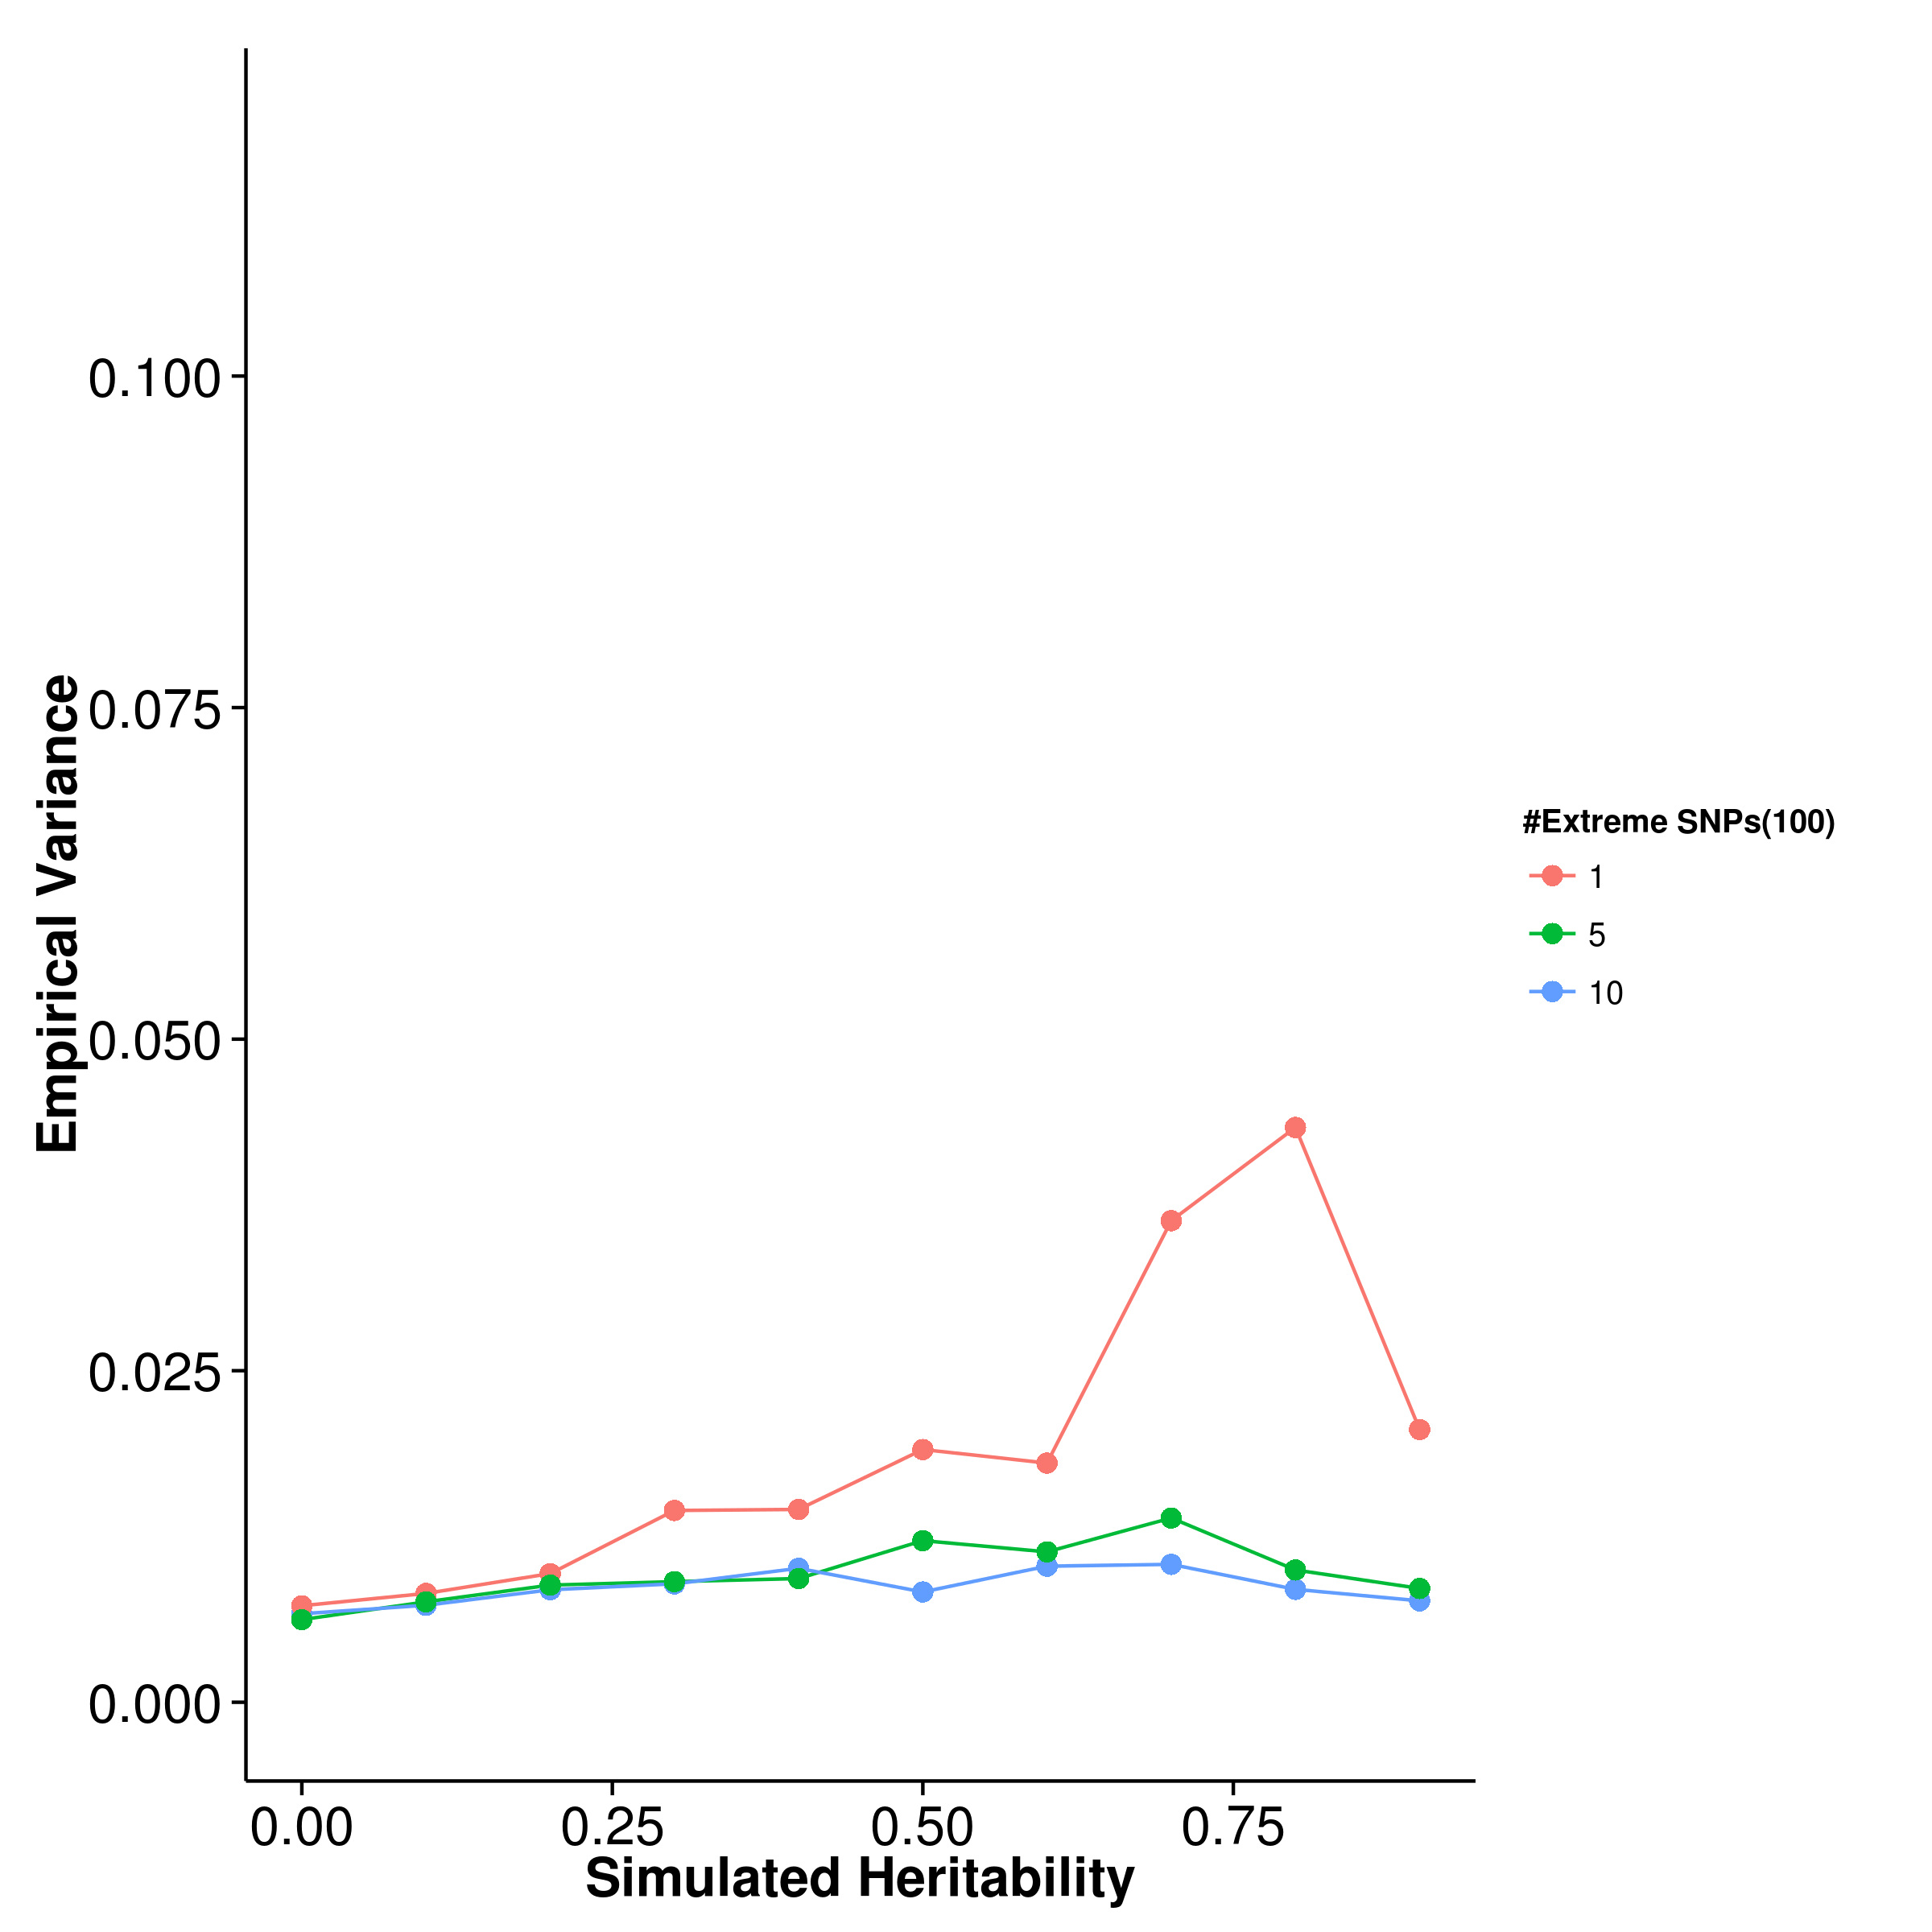
\includegraphics{figure/he_summary/extreme_100c/gcta_QtE_Rand_sd.png}}
		\label{fig:gctaQtEx100cVar}
	}\\
	\subfloat[LDSC with fix intercept]{
		\scalebox{.4}{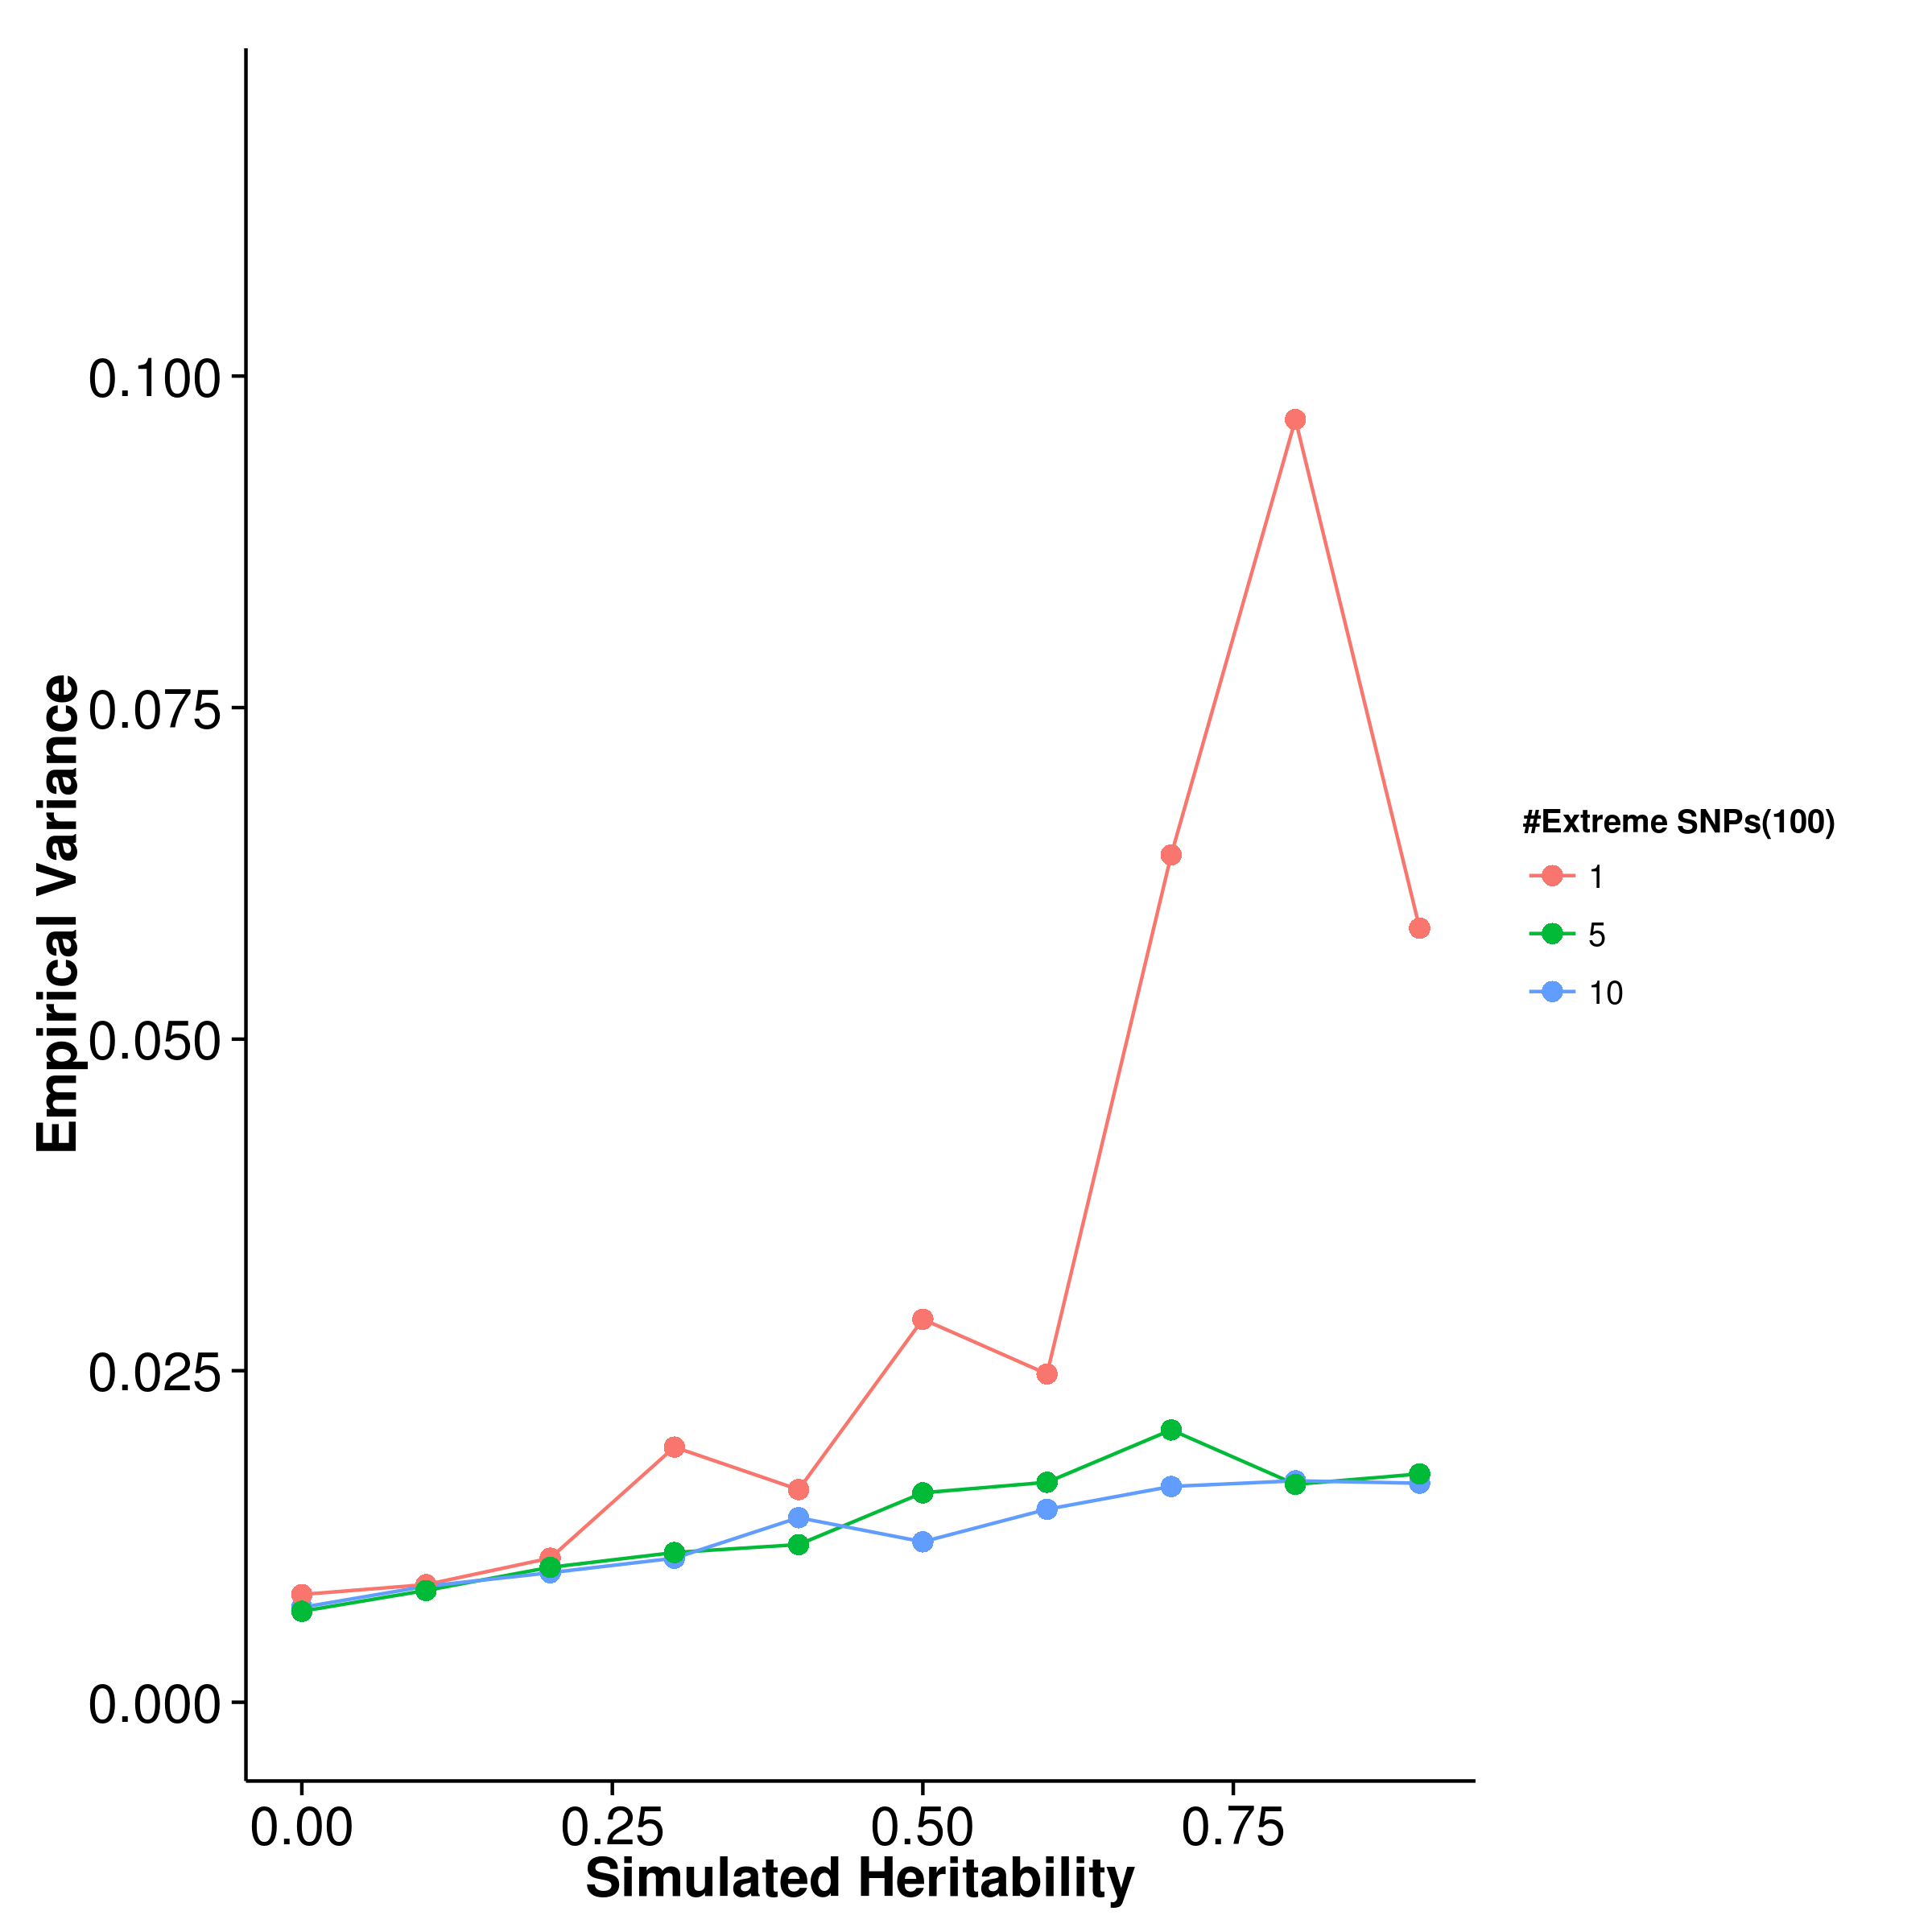
\includegraphics{figure/he_summary/extreme_100c/ldsc_QtE_Rand_sd.png}}
		\label{fig:ldscQtEx100cVar}
	}
	\subfloat[LDSC with intercept estimation]{
		
		\scalebox{.4}{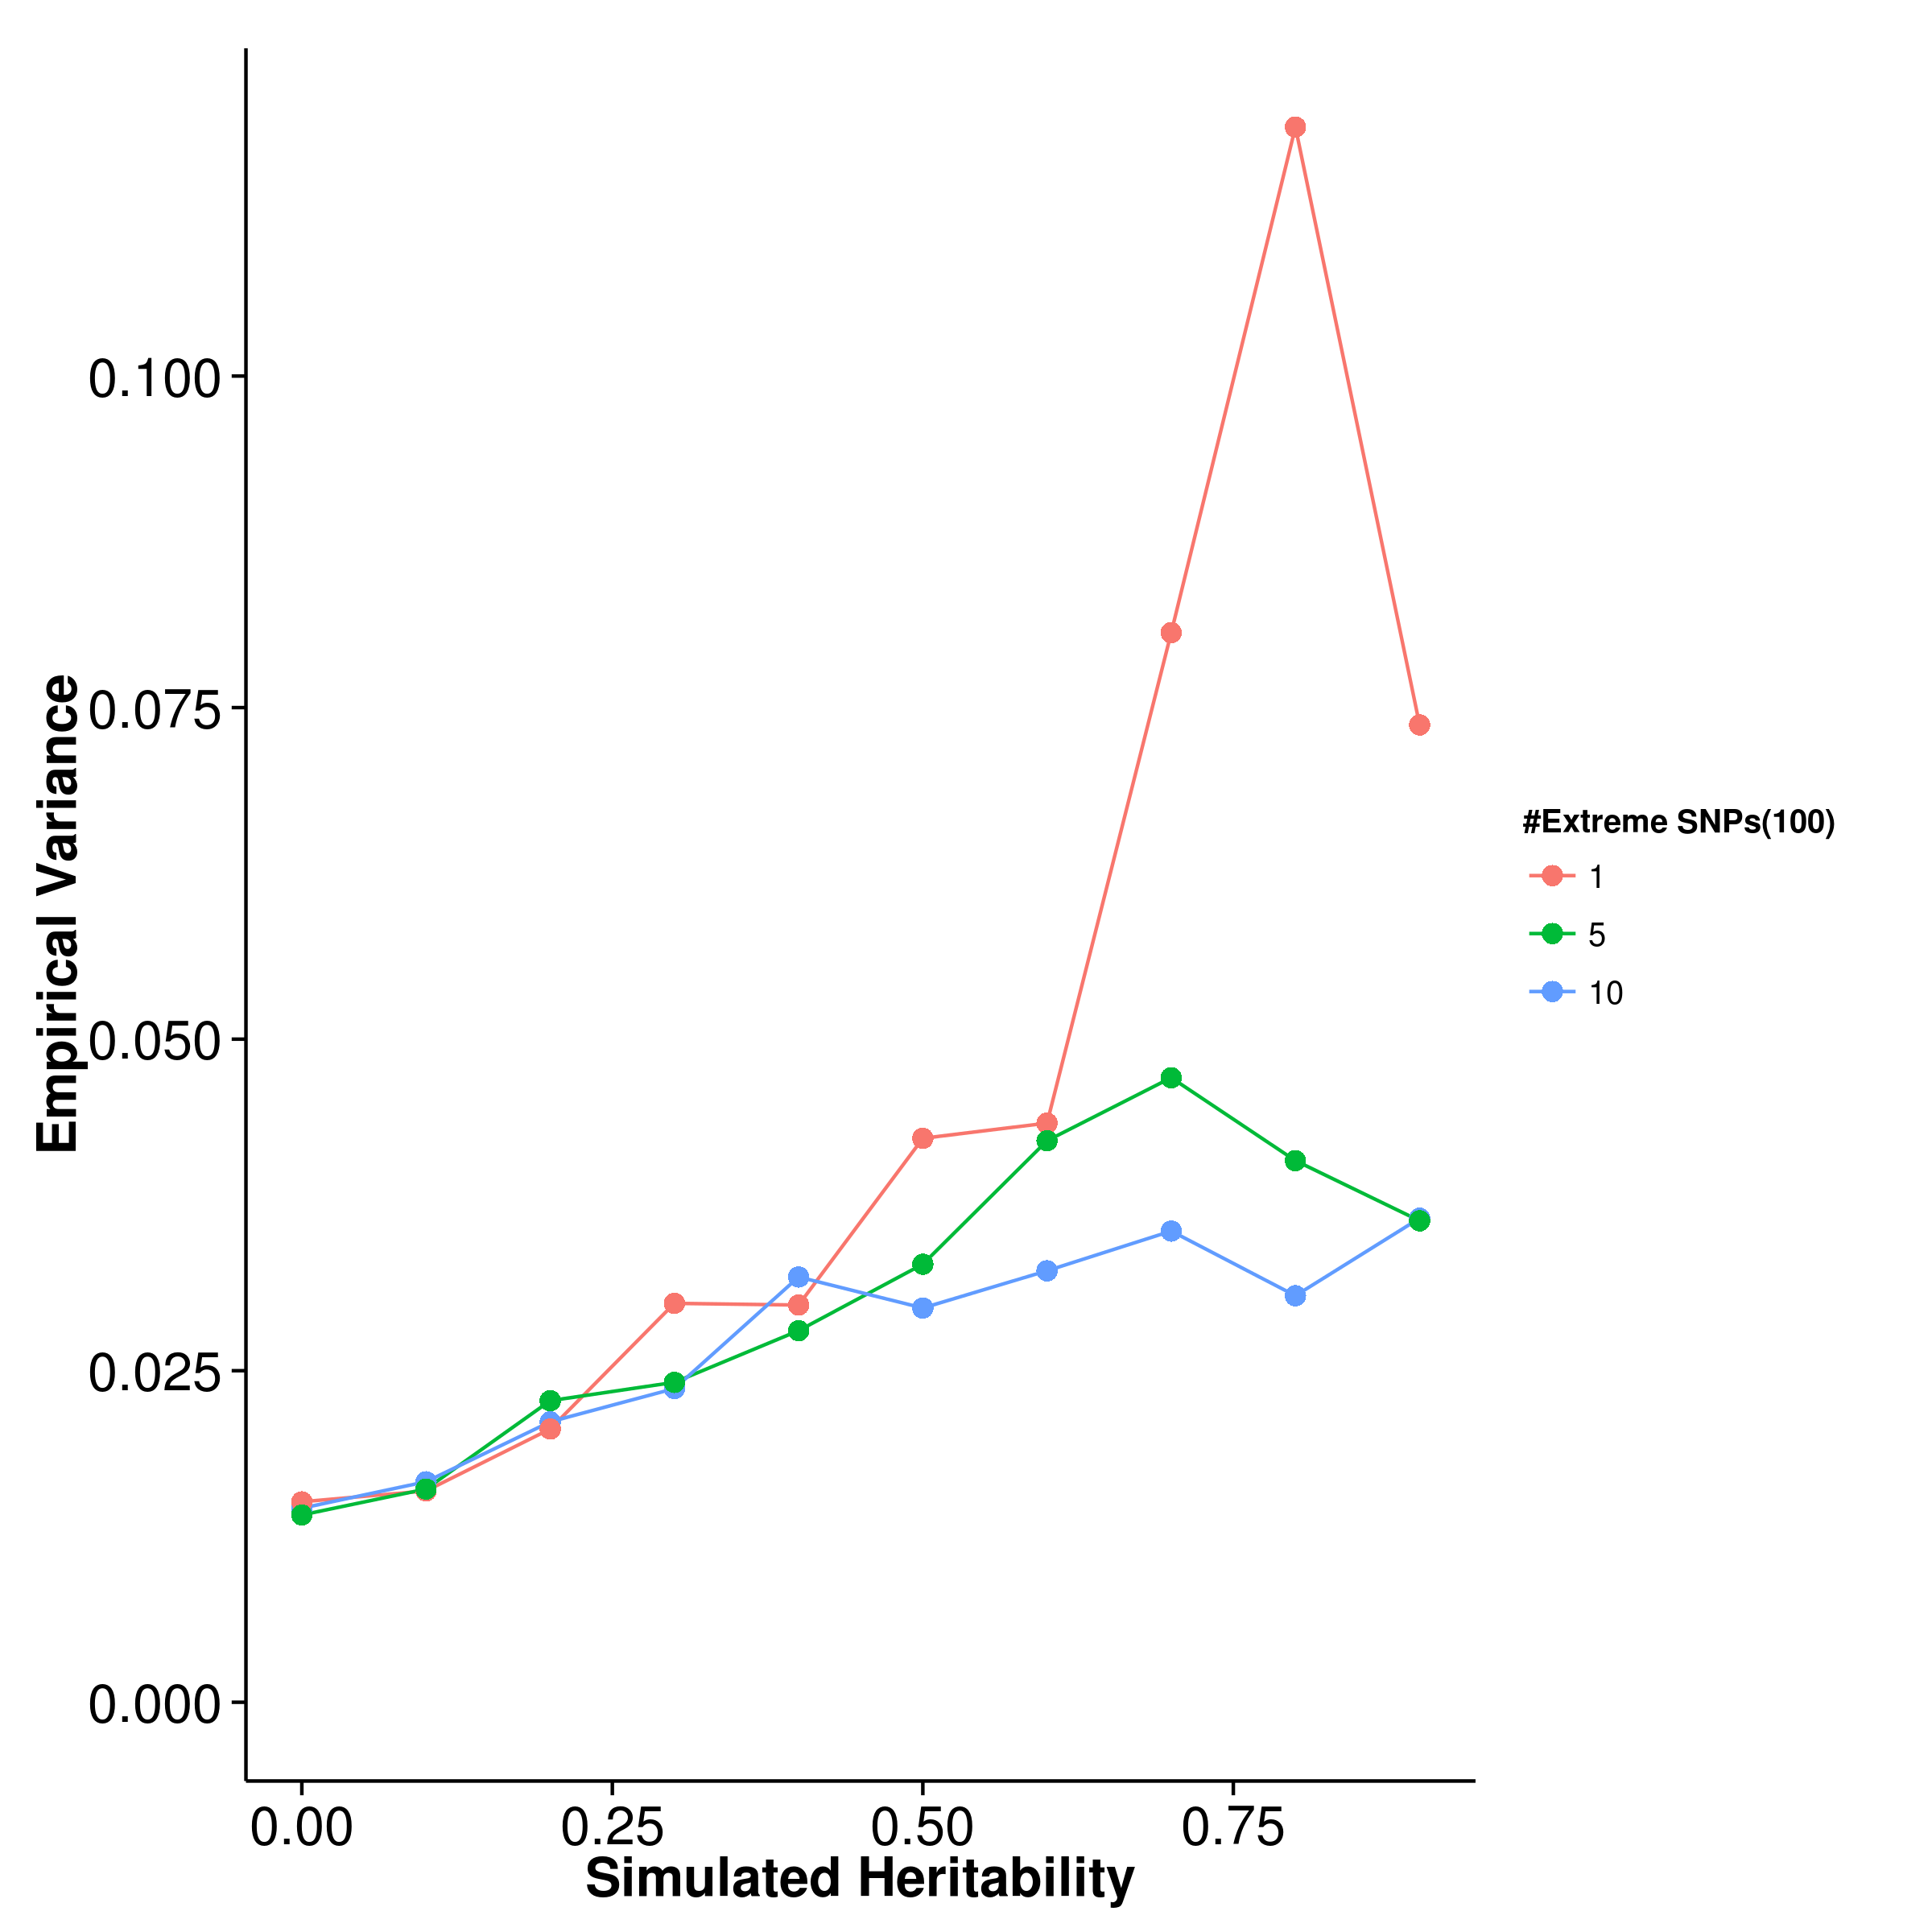
\includegraphics{figure/he_summary/extreme_100c/ldscIn_QtE_Rand_sd.png}}
		\label{fig:ldscInQtEx100cVar}
	}
	\caption[Variance of Extreme Effect Size Simulation Result]
	{Variance of results from quantitative trait simulation with extreme effect size simulation.
		100 causal \glspl{SNP} were simulated.
		When only 1 \gls{SNP} with extreme effect was simulated, the empirical variance of \gls{gcta} and \gls{ldsc} increases and a large fluctuation was observed.
		Whereas the empirical variance of \gls{shrek} only increases slightly when the simulated heritability is large and with only 1 \gls{SNP} with extreme effect.
		This suggests that \gls{shrek} is more robust to the change in number of extreme \gls{SNP}(s).
	} 
	\label{fig:QtEx100cVar}
\end{figure}
%Variance estimation
\begin{figure}
	\centering
	\subfloat[SHREK]{
		\scalebox{.4}{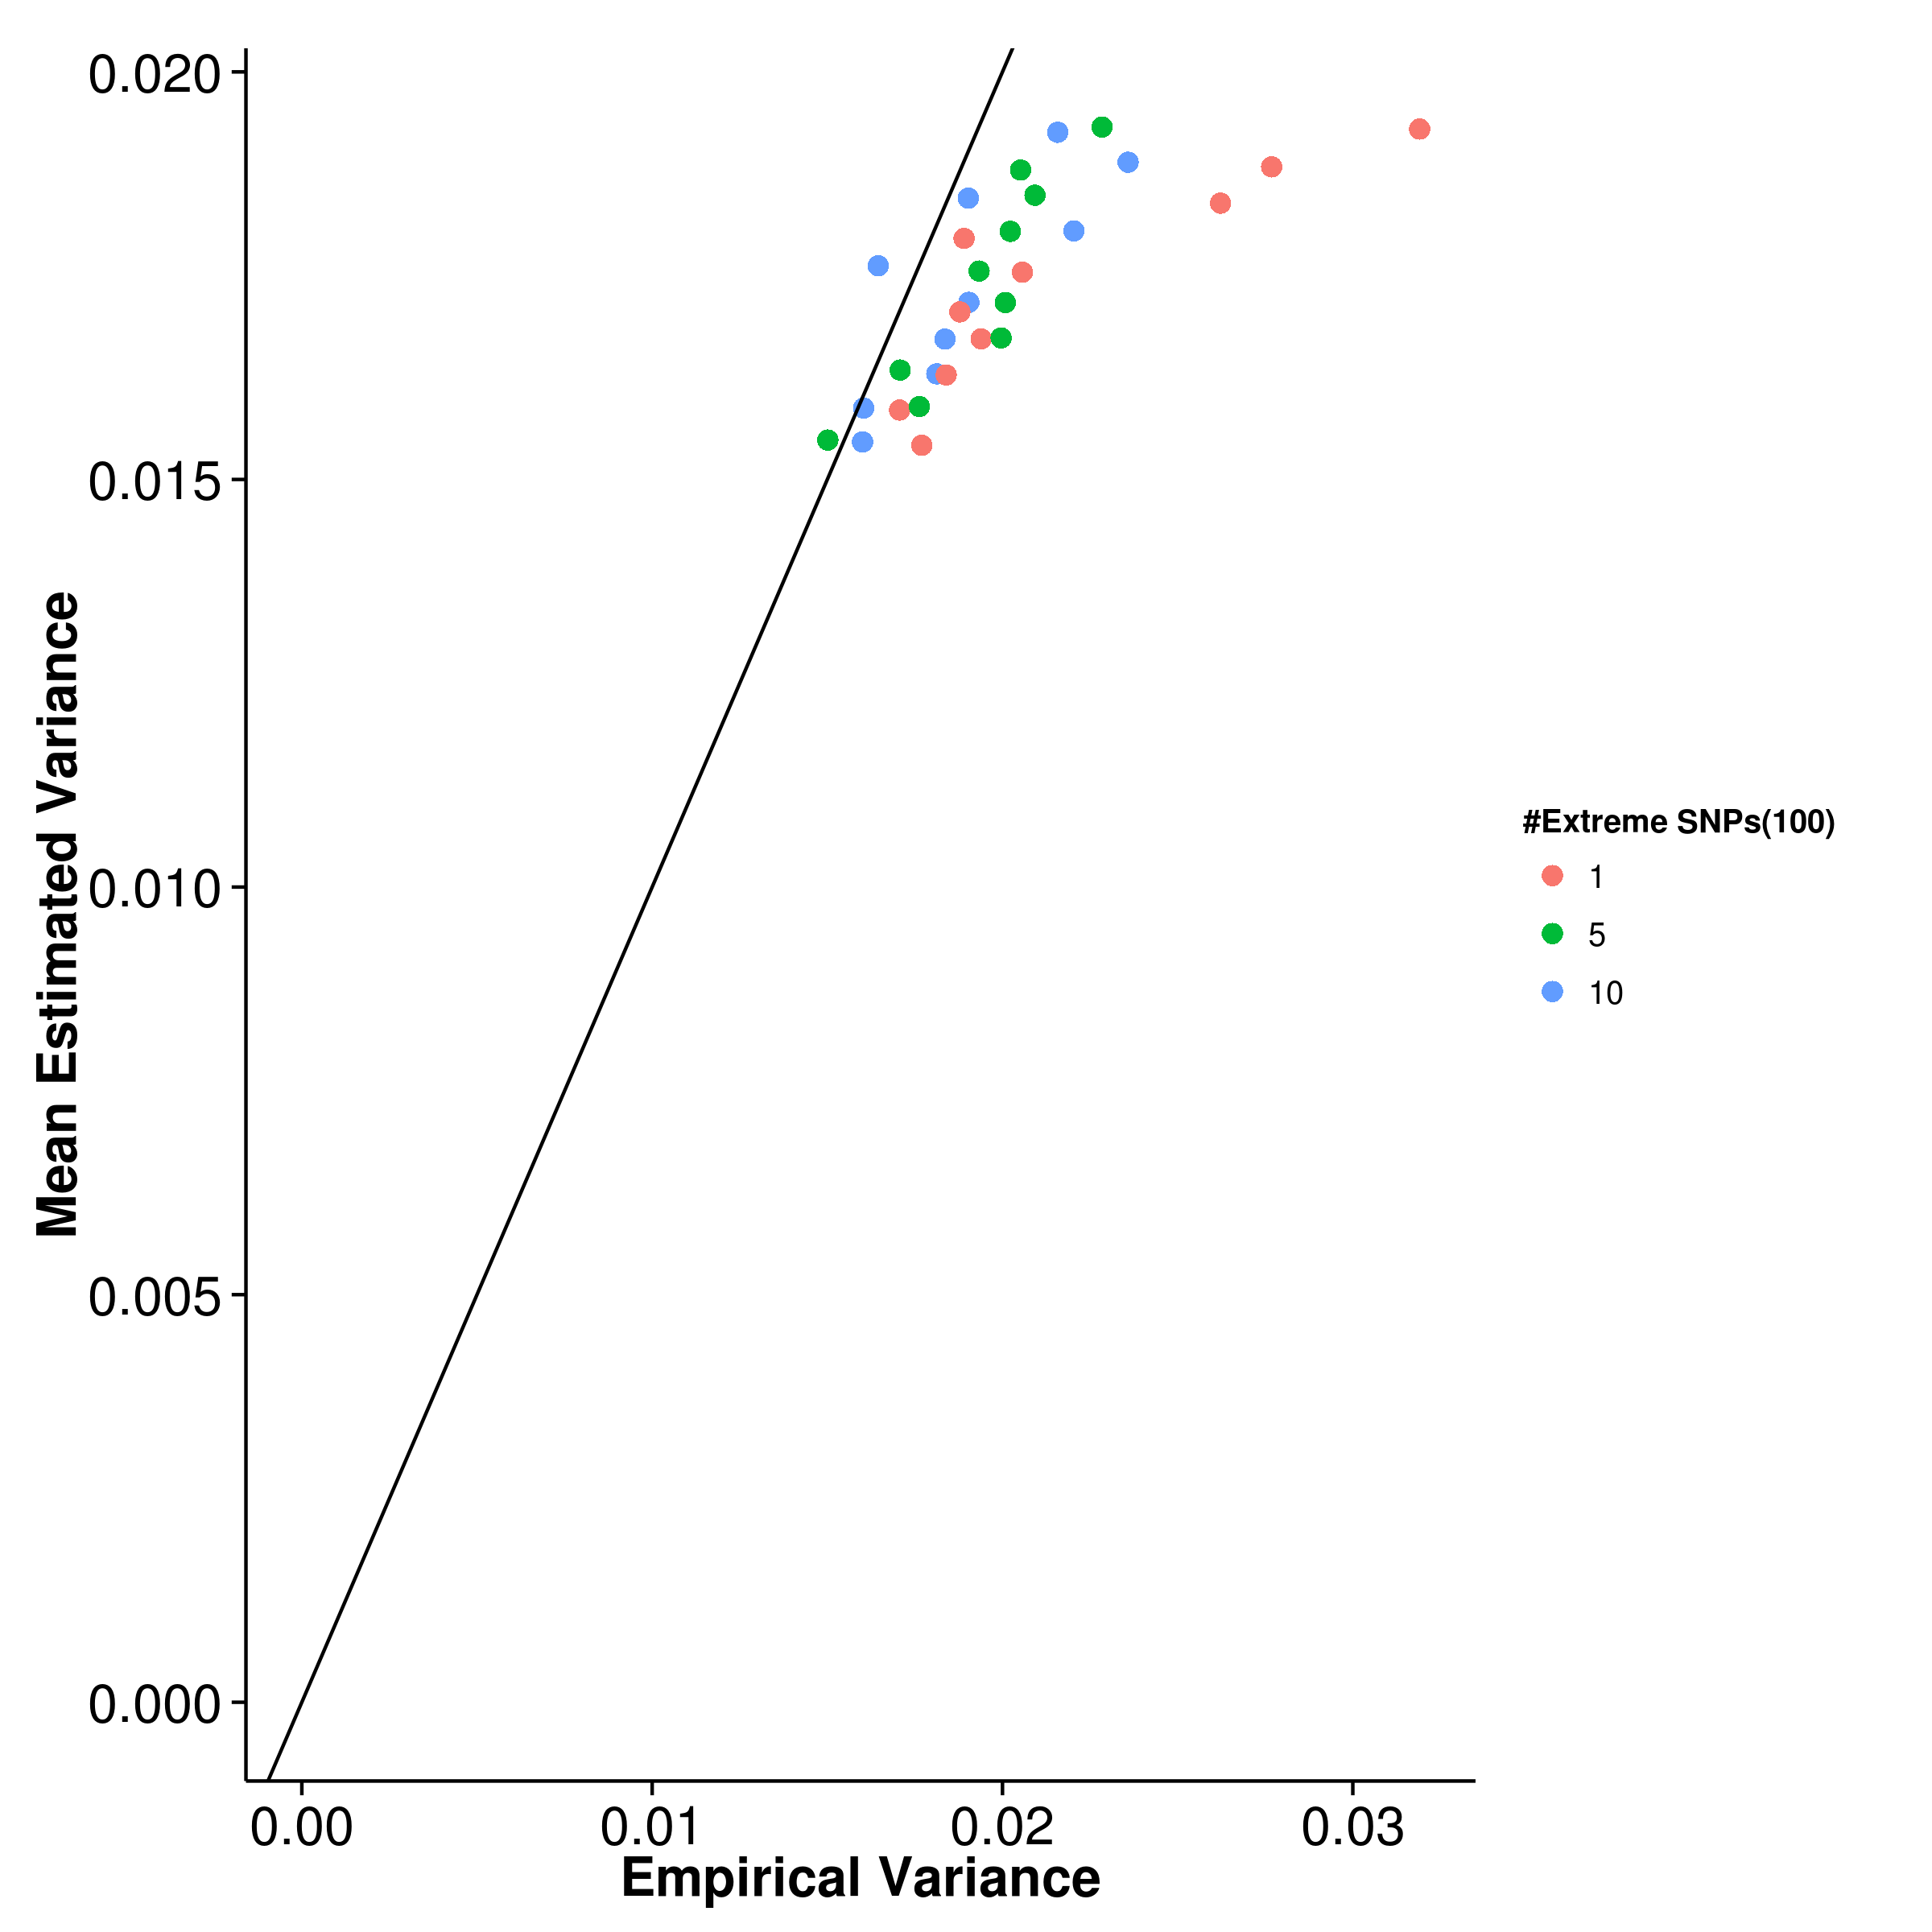
\includegraphics{figure/he_summary/extreme_100c/shrek_QtE_Rand_sdCom.png}}
		\label{fig:shrekQtEx100cVarCom}
	}
	\subfloat[GCTA]{
		\scalebox{.4}{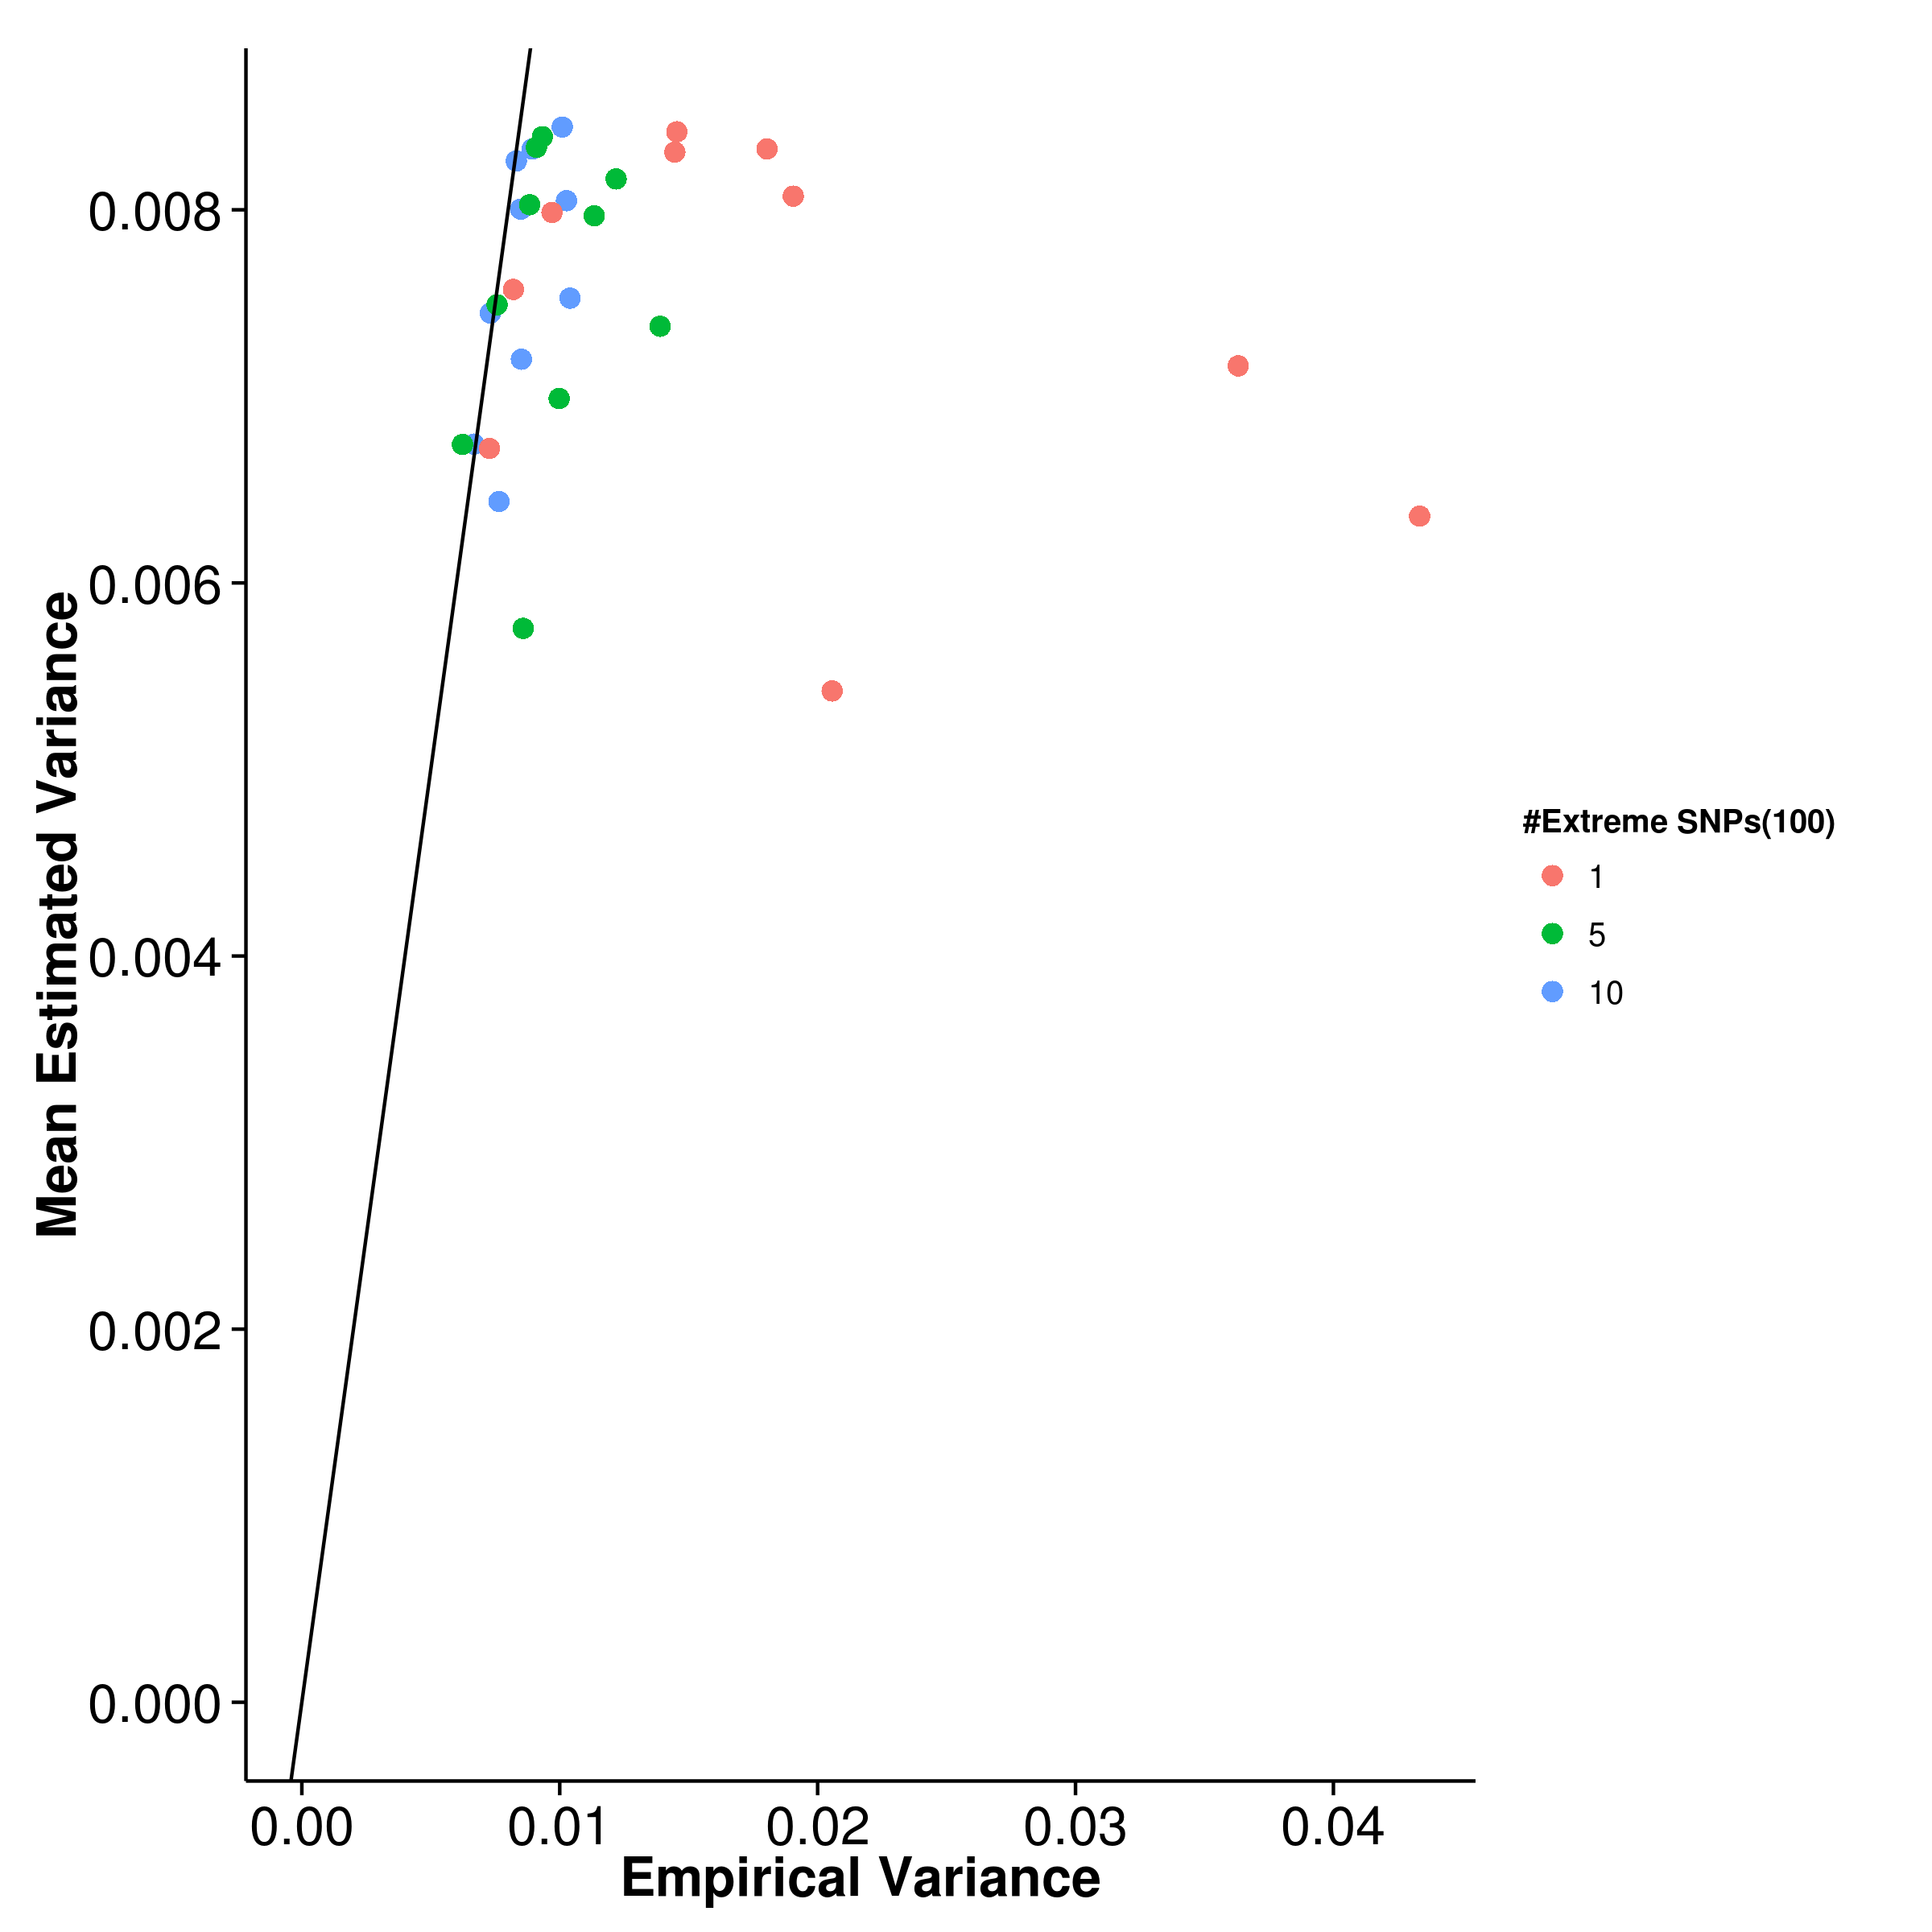
\includegraphics{figure/he_summary/extreme_100c/gcta_QtE_Rand_sdCom.png}}
		\label{fig:gctaQtEx100cVarCom}
	}\\
	\subfloat[LDSC with fix intercept]{
		\scalebox{.4}{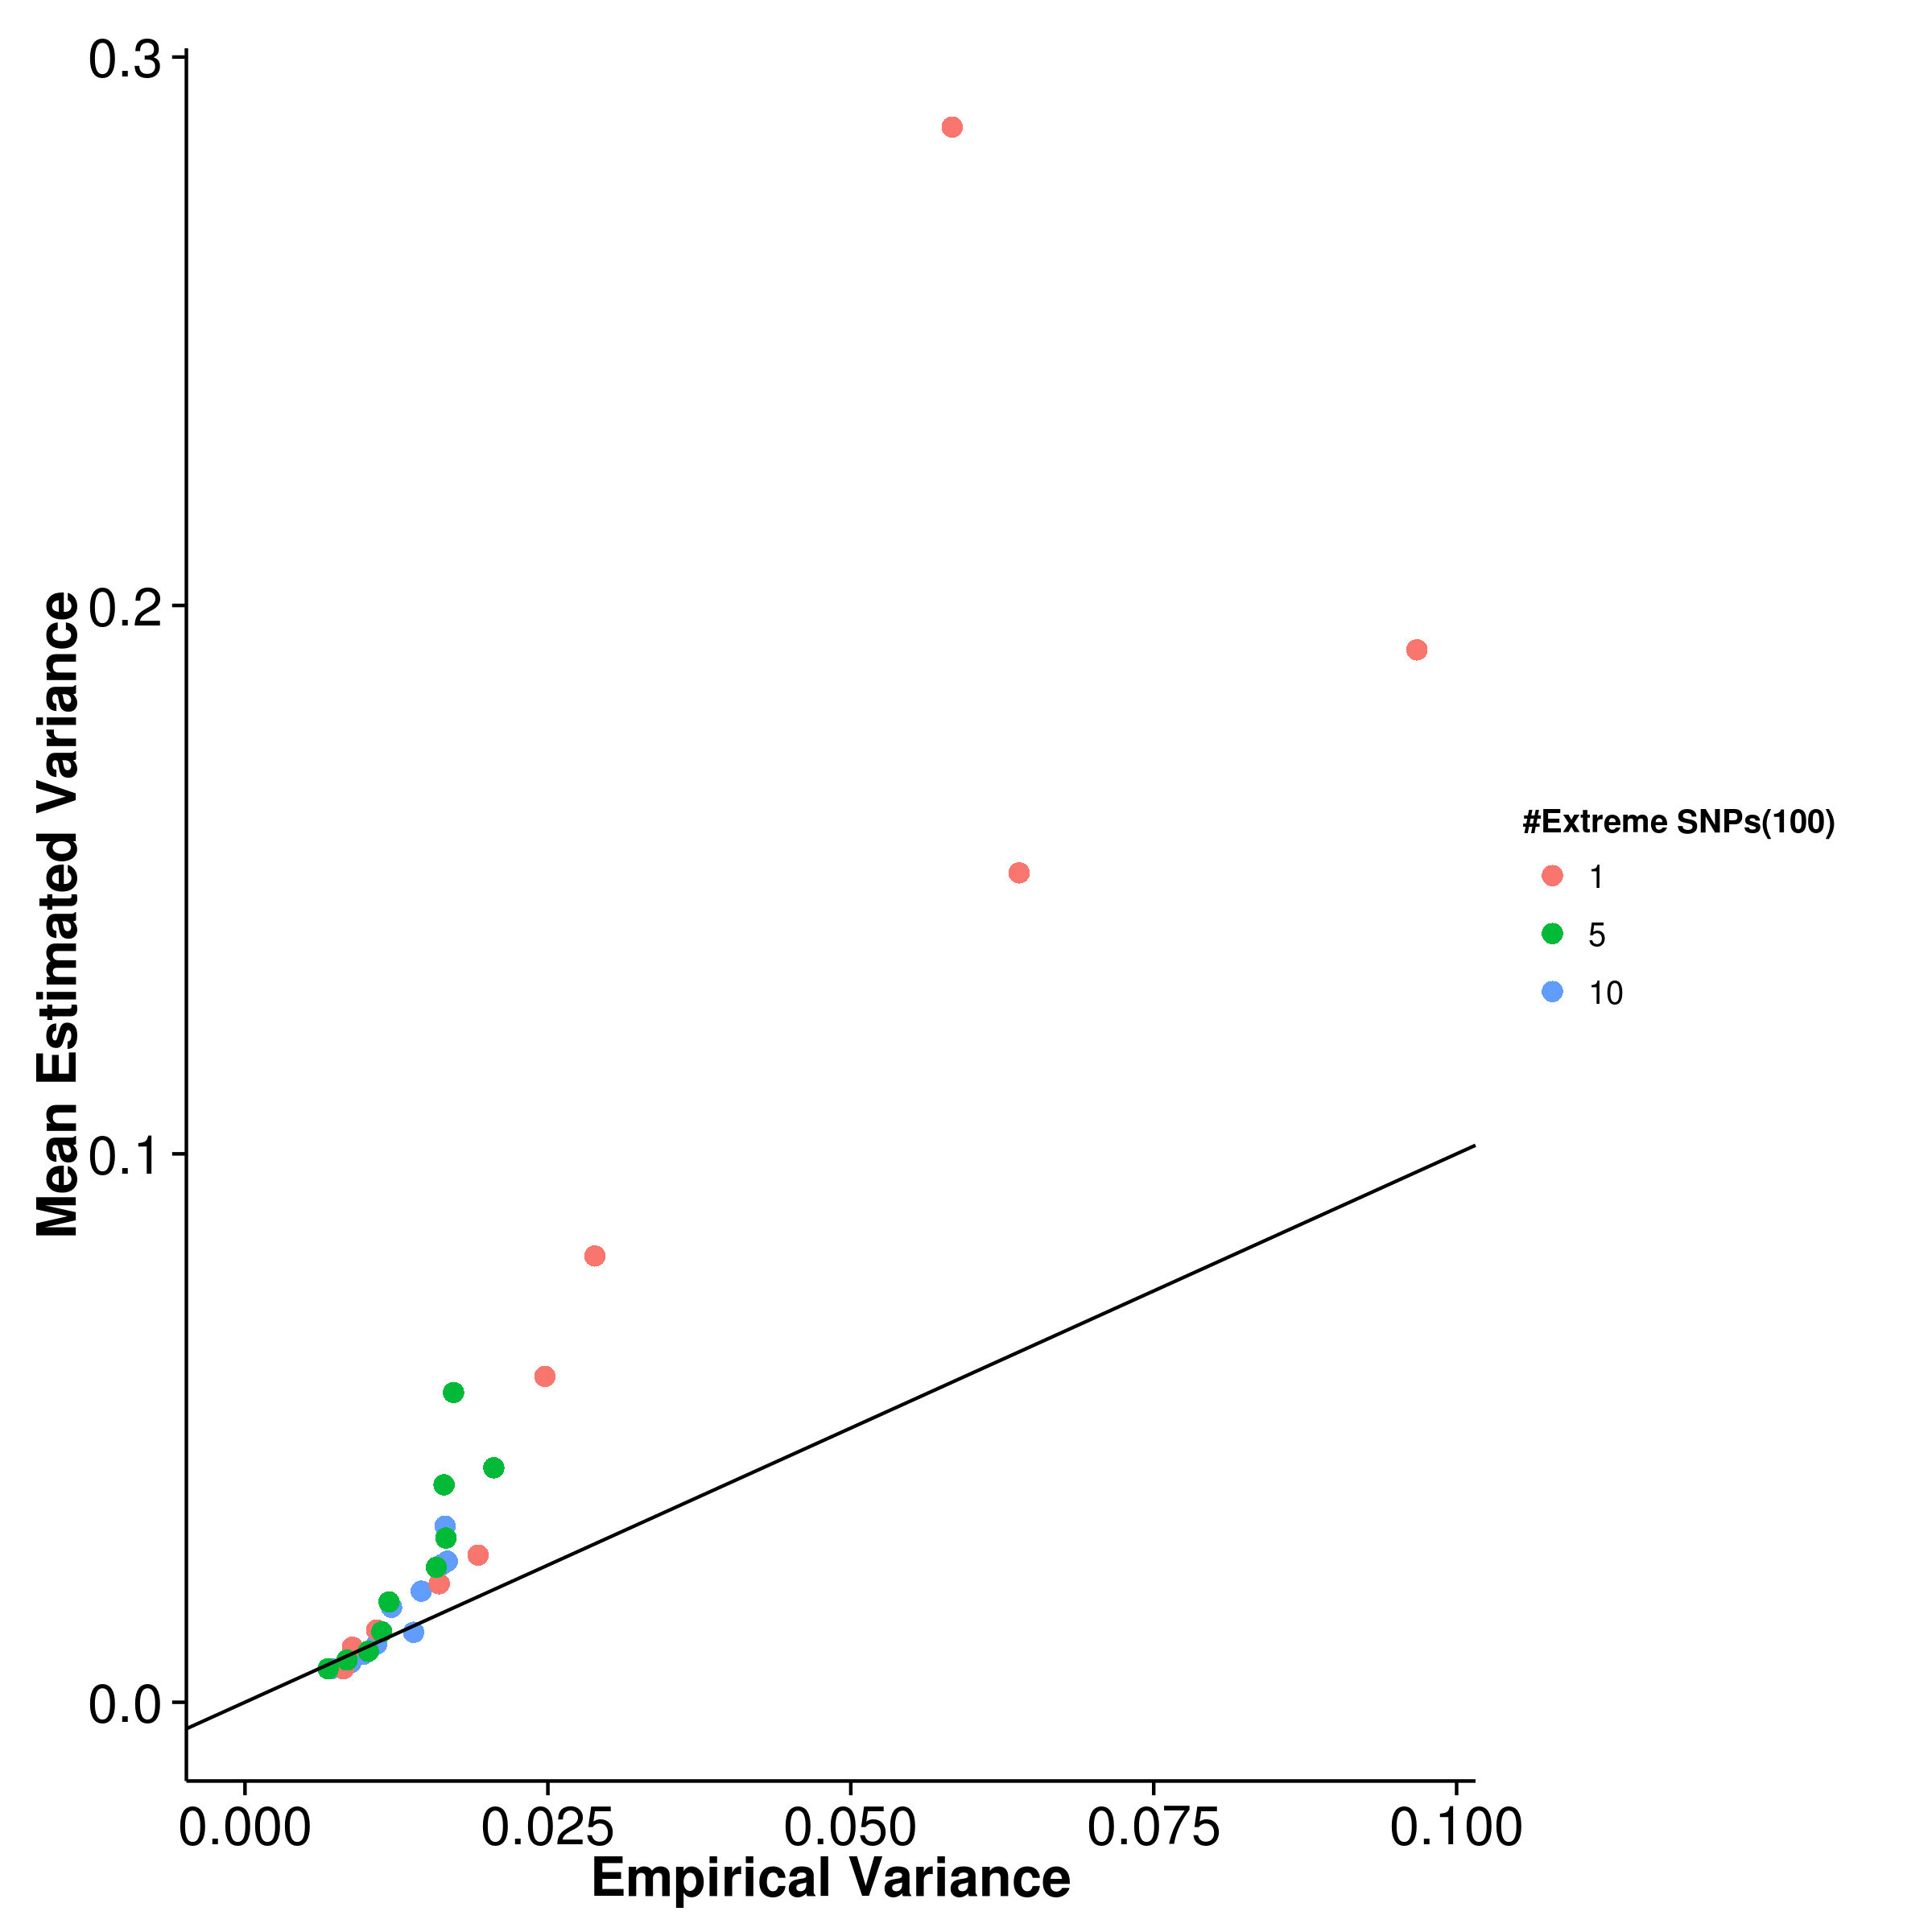
\includegraphics{figure/he_summary/extreme_100c/ldsc_QtE_Rand_sdCom.png}}
		\label{fig:ldscQtEx100cVarCom}
	}
	\subfloat[LDSC with intercept estimation]{
		
		\scalebox{.4}{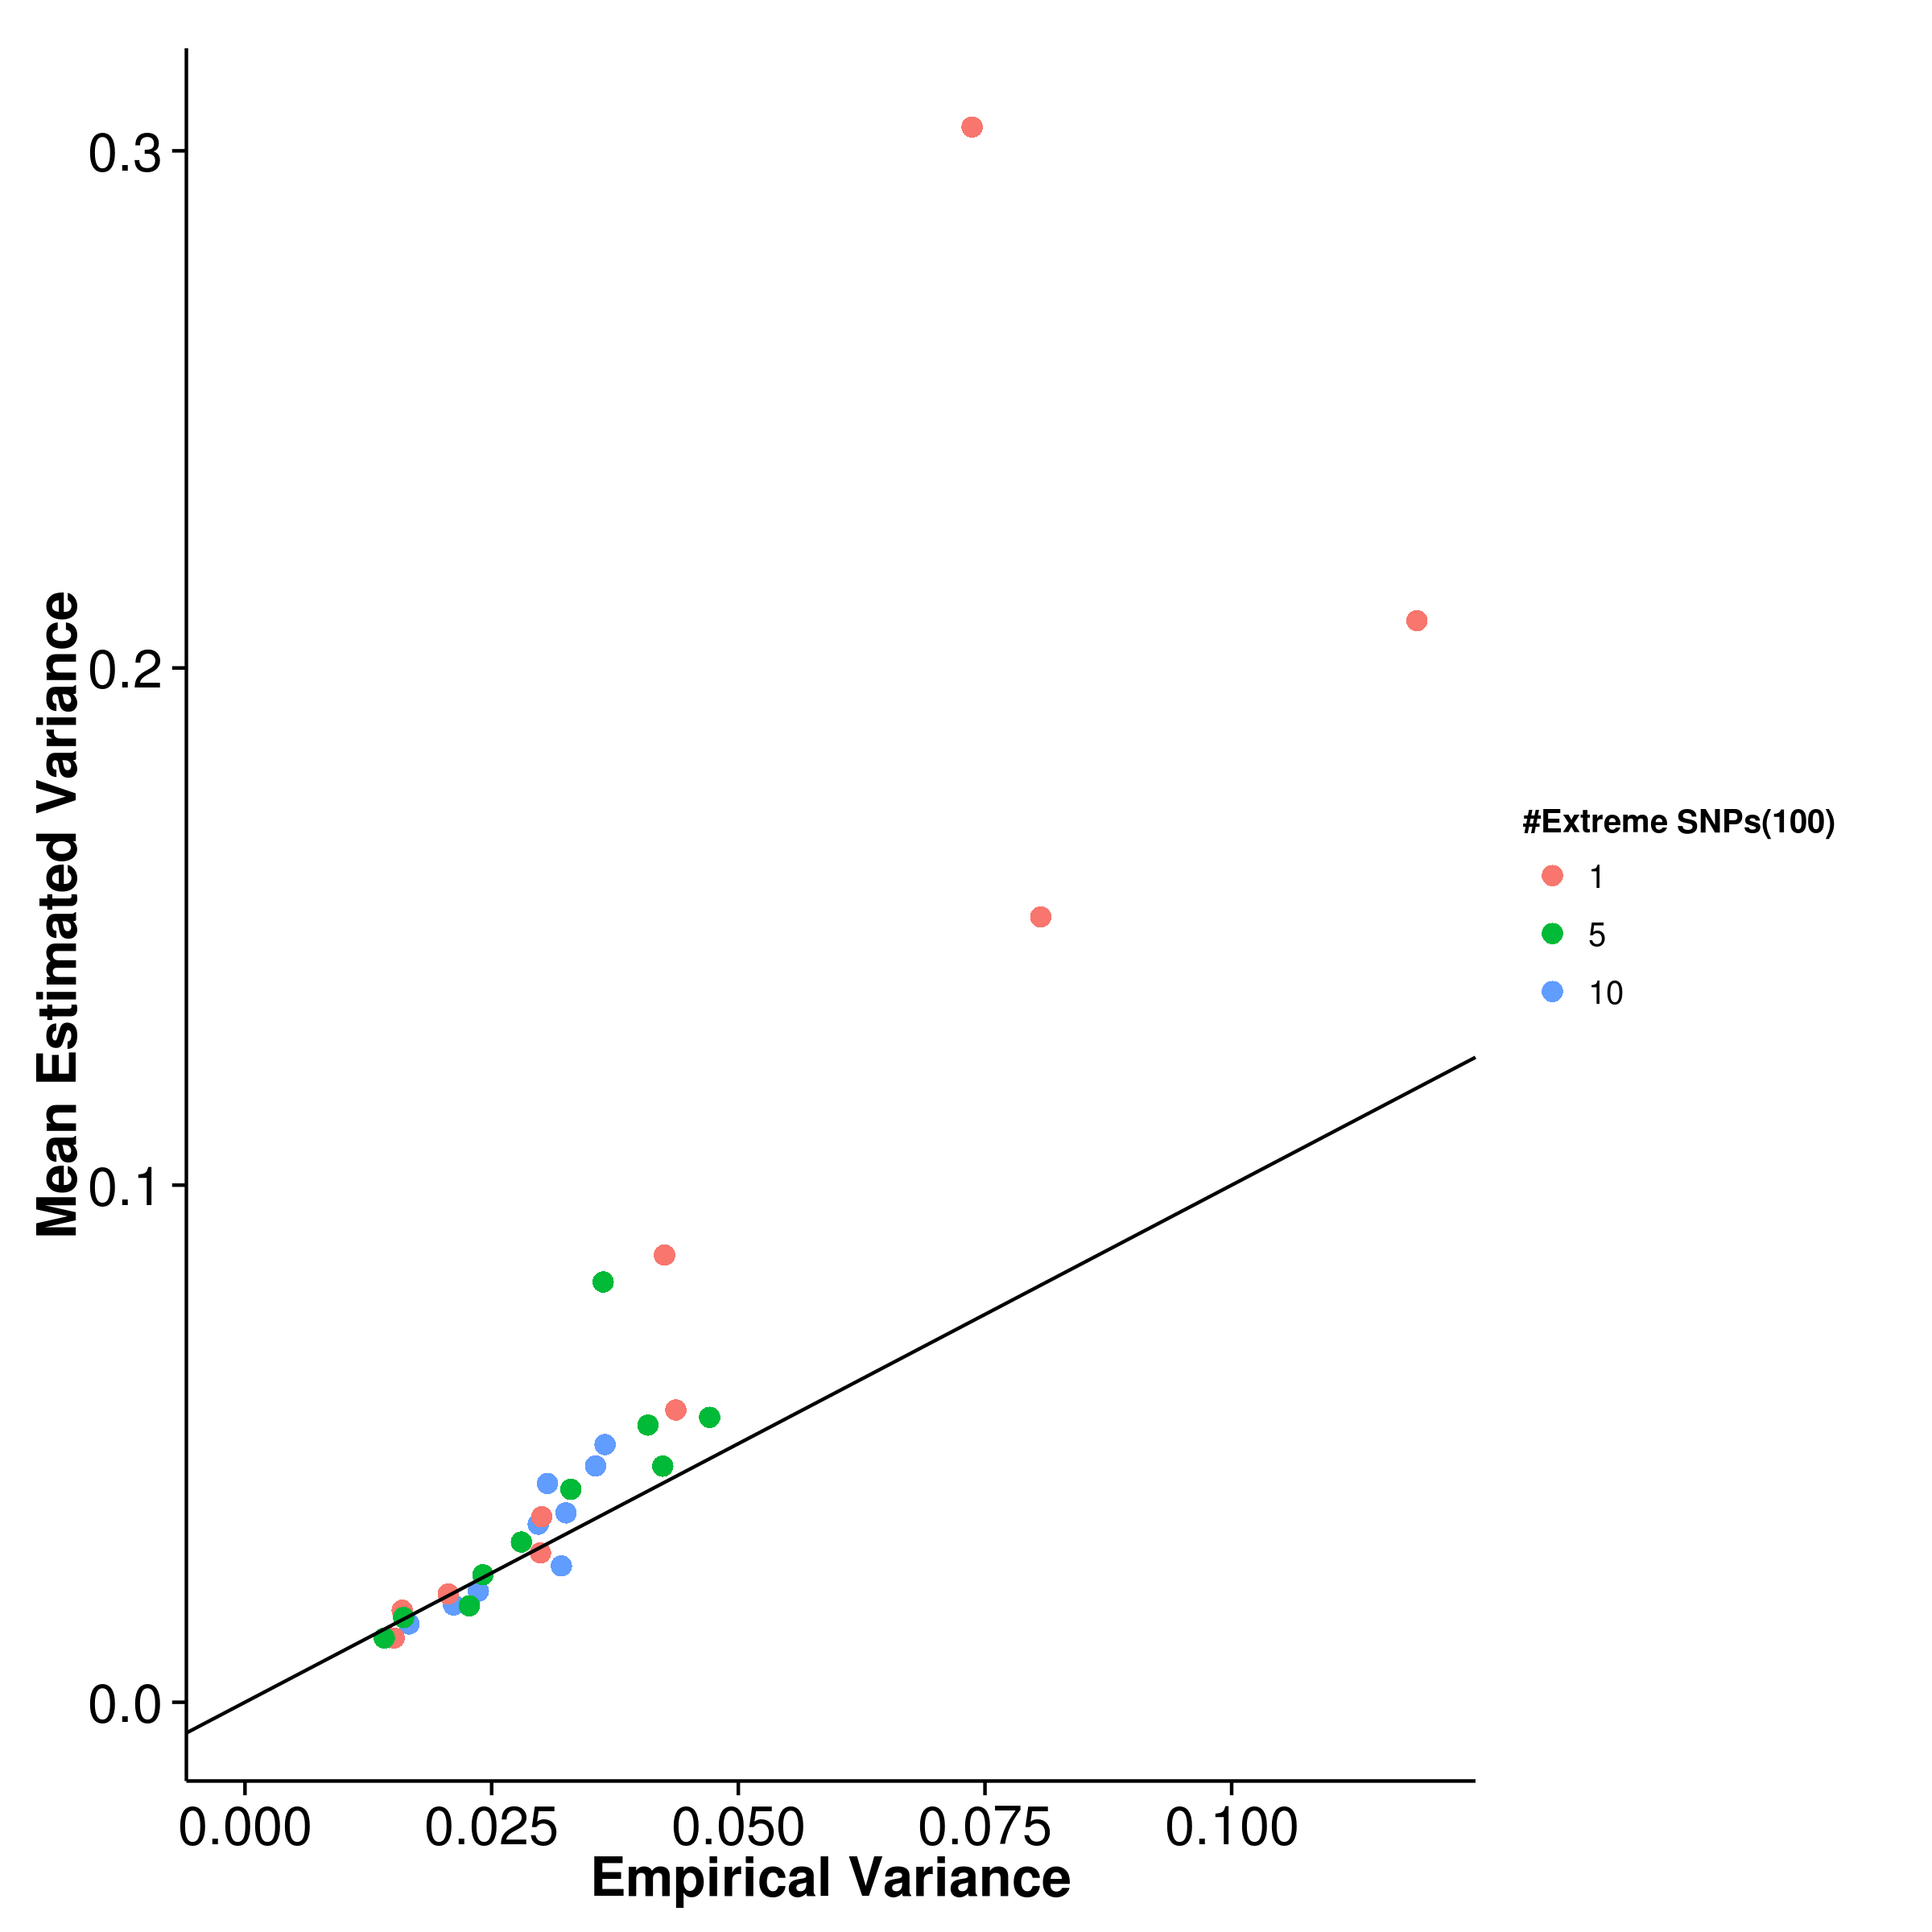
\includegraphics{figure/he_summary/extreme_100c/ldscIn_QtE_Rand_sdCom.png}}
		\label{fig:ldscInQtEx100cVarCom}
	}
	\caption[Estimation of Variance in Extreme Effect Size Simulation]
	{Estimated variance of results from quantitative trait simulation with extreme effect size simulation when compared to the empirical variance.
		100 causal \glspl{SNP} were simulated.
		\gls{shrek} and \gls{gcta} generally under-estimate the variance with the magnitude of bias being the highest when there is only 1 \gls{SNP} with extreme effect.
		On the other hand, \gls{ldsc} tends to over-estimate the variance and it can overestimate the variance by more than 3 folds when there is only 1 \gls{SNP} with extreme effect.
	} 
	\label{fig:QtEx100cVarCom}
\end{figure}

Sometimes, it is possible for a trait to have a small portion of causal variants with much larger effect size when compared to other causal variants.
To investigate how \gls{ldsc} and \gls{shrek} perform in such scenarios, simulations were performed with trait that has 100 causal \glspl{SNP} where 1,5 or 10 of those \gls{SNP}(s) has a large effect.

The overall performance of the algorithms are similar to the results observed in the quantitative trait simulation (\cref{fig:QtEx100cMean}).
However, when 1 of the causal \glspl{SNP} was simulated with large effect, the mean estimates from \gls{ldsc} and \gls{gcta} fluctuate (\cref{fig:gctaQtEx100cMean,fig:ldscQtEx100cMean,fig:ldscInQtEx100cMean}).
The same fluctuation is not observed in \gls{shrek} (\cref{fig:shrekQtEx100cMean}). 
Similarly, the empirical variance of the estimates (\cref{fig:QtEx100cVar}) from \gls{gcta} and \gls{ldsc} increase and fluctuate when only 1 of the causal \glspl{SNP} was simulated with large effect.
Again, the estimates from \gls{shrek} are robust to change in number of \gls{SNP} with large effect size.

When inspecting the variance estimation, it is observed that both \gls{shrek} and \gls{gcta} underestimate their empirical variance. 
As the number of \gls{SNP}(s) with large effect size decreases, the magnitude of bias increases.
On the other hand, it is observed that \gls{ldsc} tends to overestimate its empirical variance. 
When the intercept is fixed, the estimated variance from \gls{ldsc} can be as much as 3 fold larger than the empirical variance when only 1 of the causal \gls{SNP} with large effect size was simulated. 

To conclude, \gls{gcta} has the best performance among the algorithms tested (\cref{tab:mseEx100c}).
However, in the case where the individual genotypes are not available, \gls{shrek} has a better performance when compared to \gls{ldsc} when only 1 of the causal \glspl{SNP} carries a large effect size.
Moreover, it is also observed that \gls{shrek} is more robust to change in number of \glspl {SNP} with large effect size. 

\begin{table}
	\centering
	\begin{tabular}{rrrrr}
		\toprule
		Number of Extreme SNPs&	SHREK&	LDSC&	LDSC-In&	GCTA \\
		\midrule
		1	&	0.0227	&	0.0393	&	0.0508	&	0.0206\\
		5	&	0.0203	&	0.0145	&	0.0316	&	0.00985\\
		10	&	0.0205	&	0.0129	&	0.0329	&	0.00939\\
		\bottomrule
	\end{tabular}
	\caption[MSE of Quantitative Trait Simulation with Extreme Effect Size]{
		\gls{mse} of quantitative trait simulation with extreme effect size.
		Of all the algorithms, \gls{gcta} has the lowest \gls{mse}.
		When comparing the performance of \gls{shrek} and \gls{ldsc}, it is observed that \gls{ldsc} performs better unless only 1 of the causal \gls{SNP} has a large effect size.
		However, it is also observed that the performance of \gls{shrek} is robust to the change in number of \glspl{SNP} with extreme effect size.
	}
	\label{tab:mseEx100c}
\end{table}

\subsubsection{Binary Trait Simulation}
%Mean
\begin{figure}
	\centering
	\subfloat[SHREK]{
		\scalebox{.4}{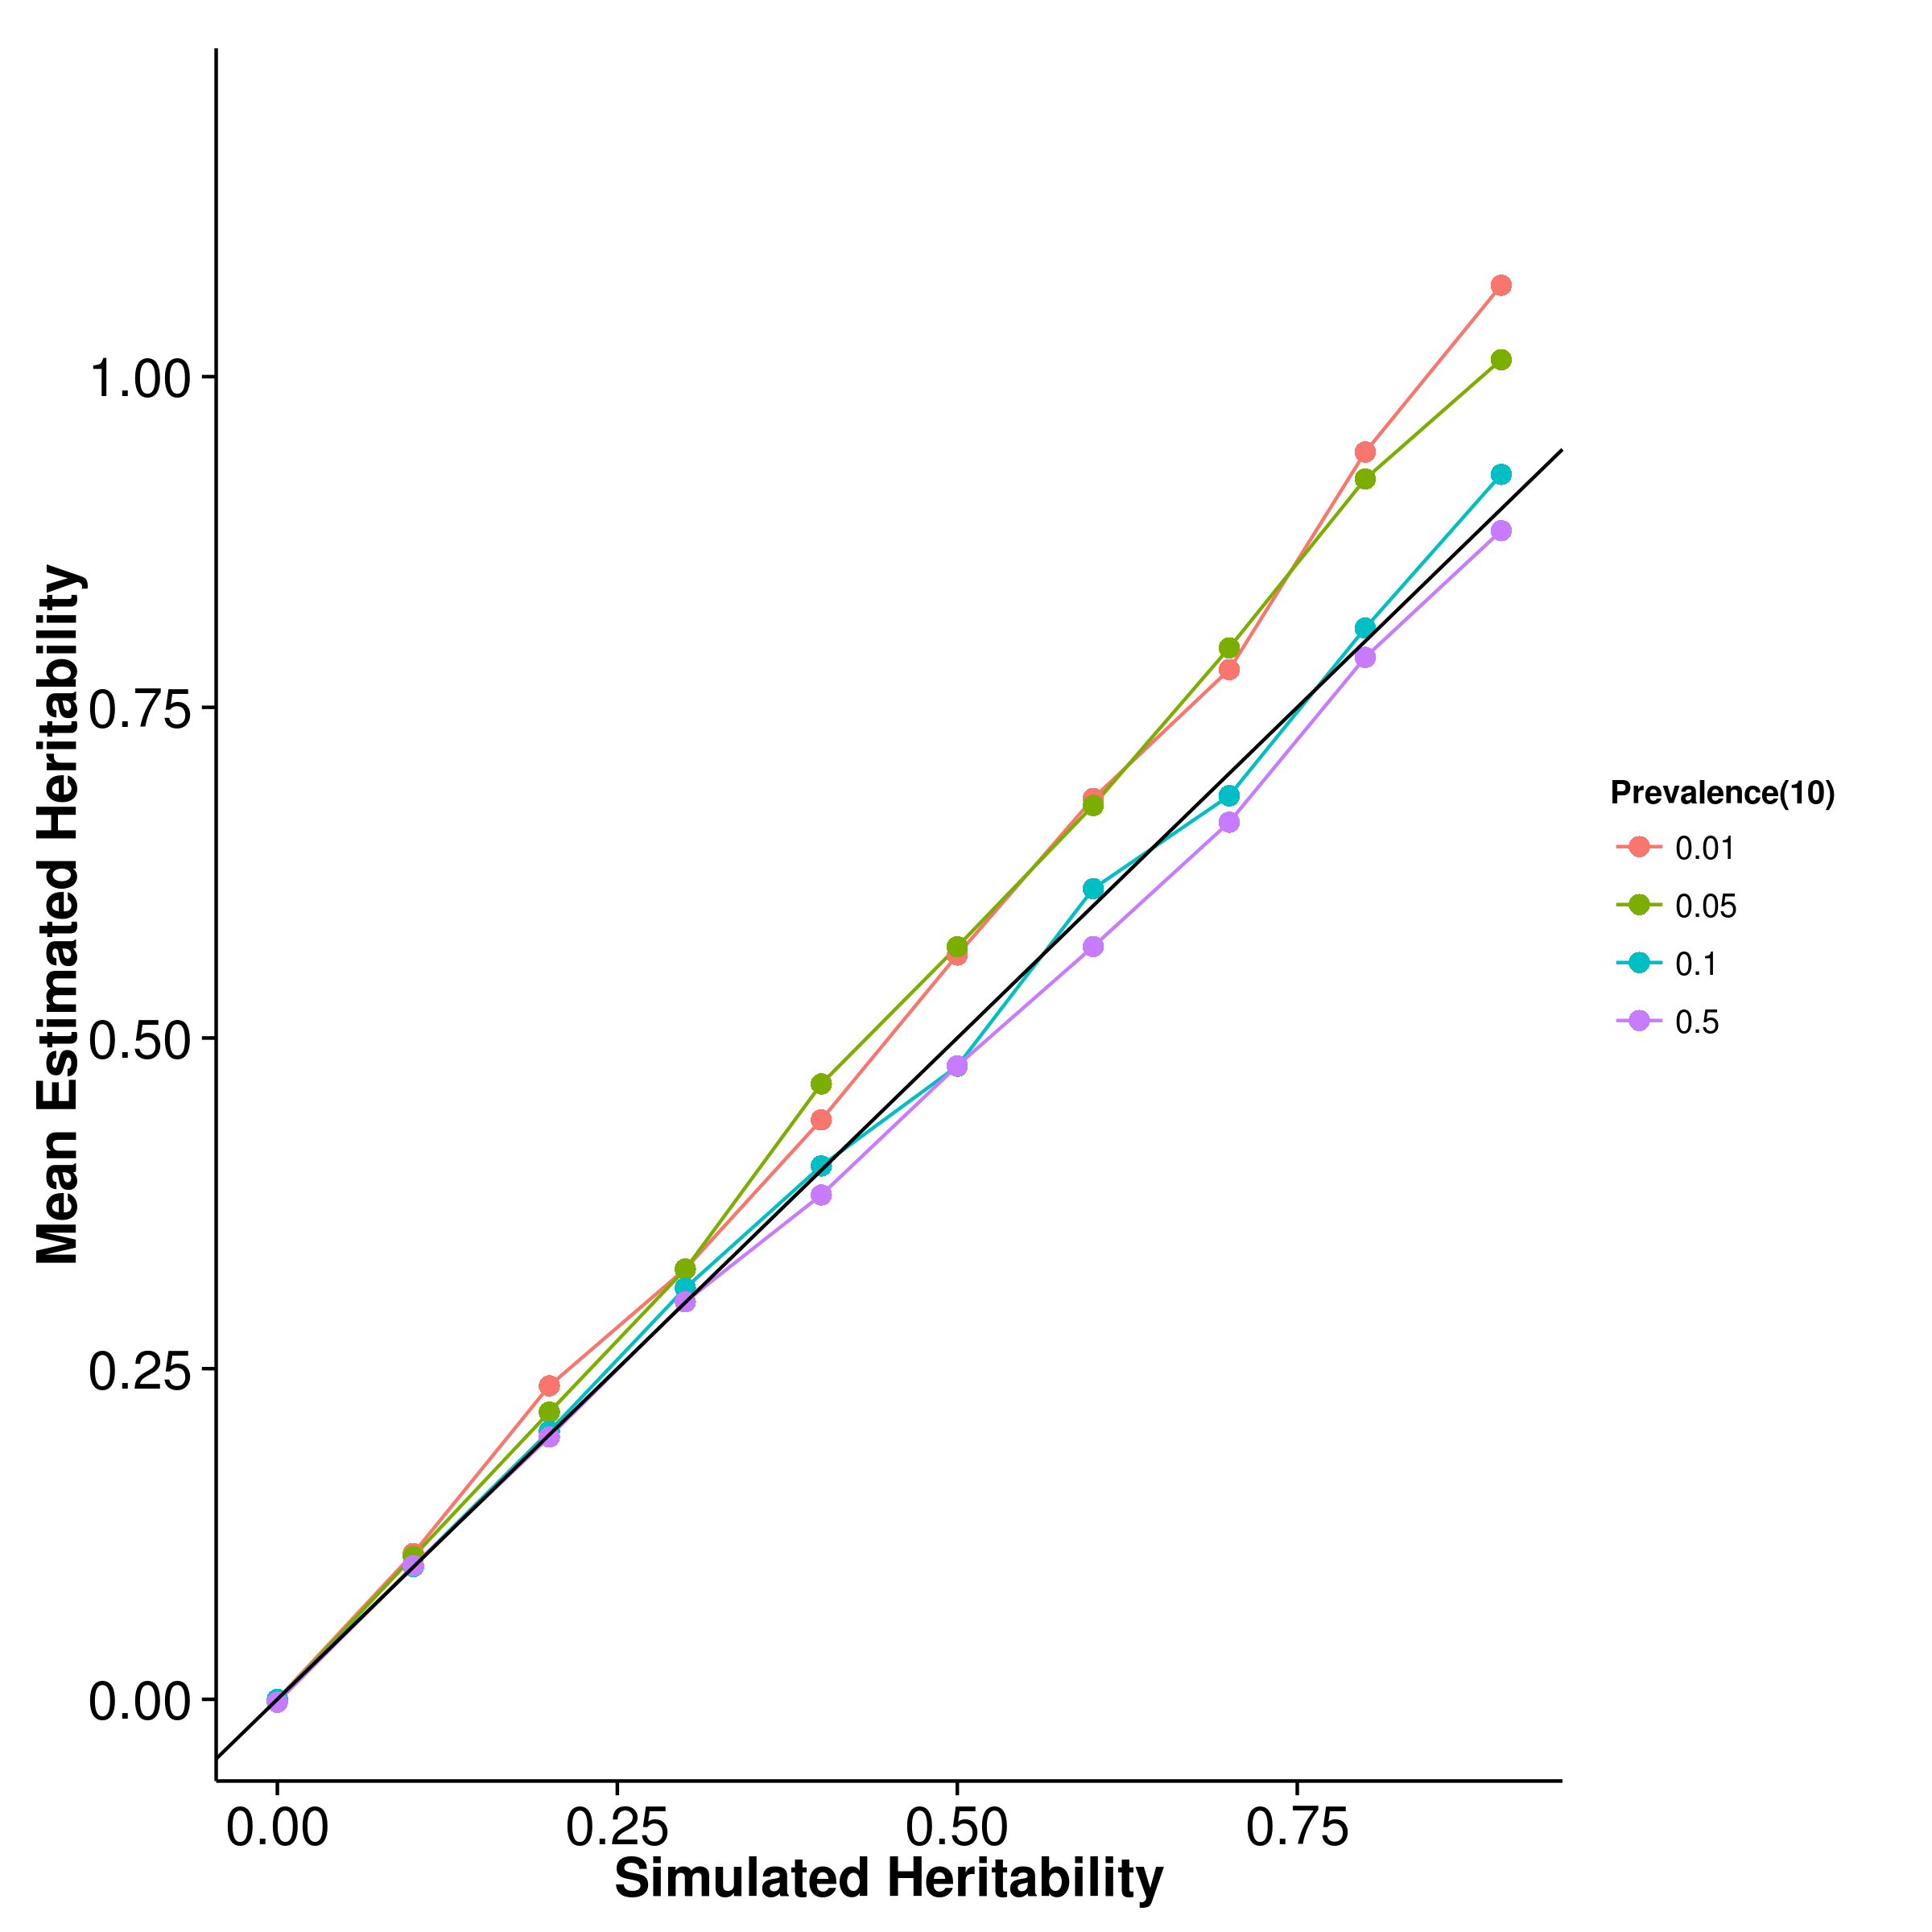
\includegraphics{figure/he_summary/cc_10c/shrek_CC_Rand_mean.png}}
		\label{fig:shrekCC10RandMean}
	}
	\subfloat[GCTA]{
		\scalebox{.4}{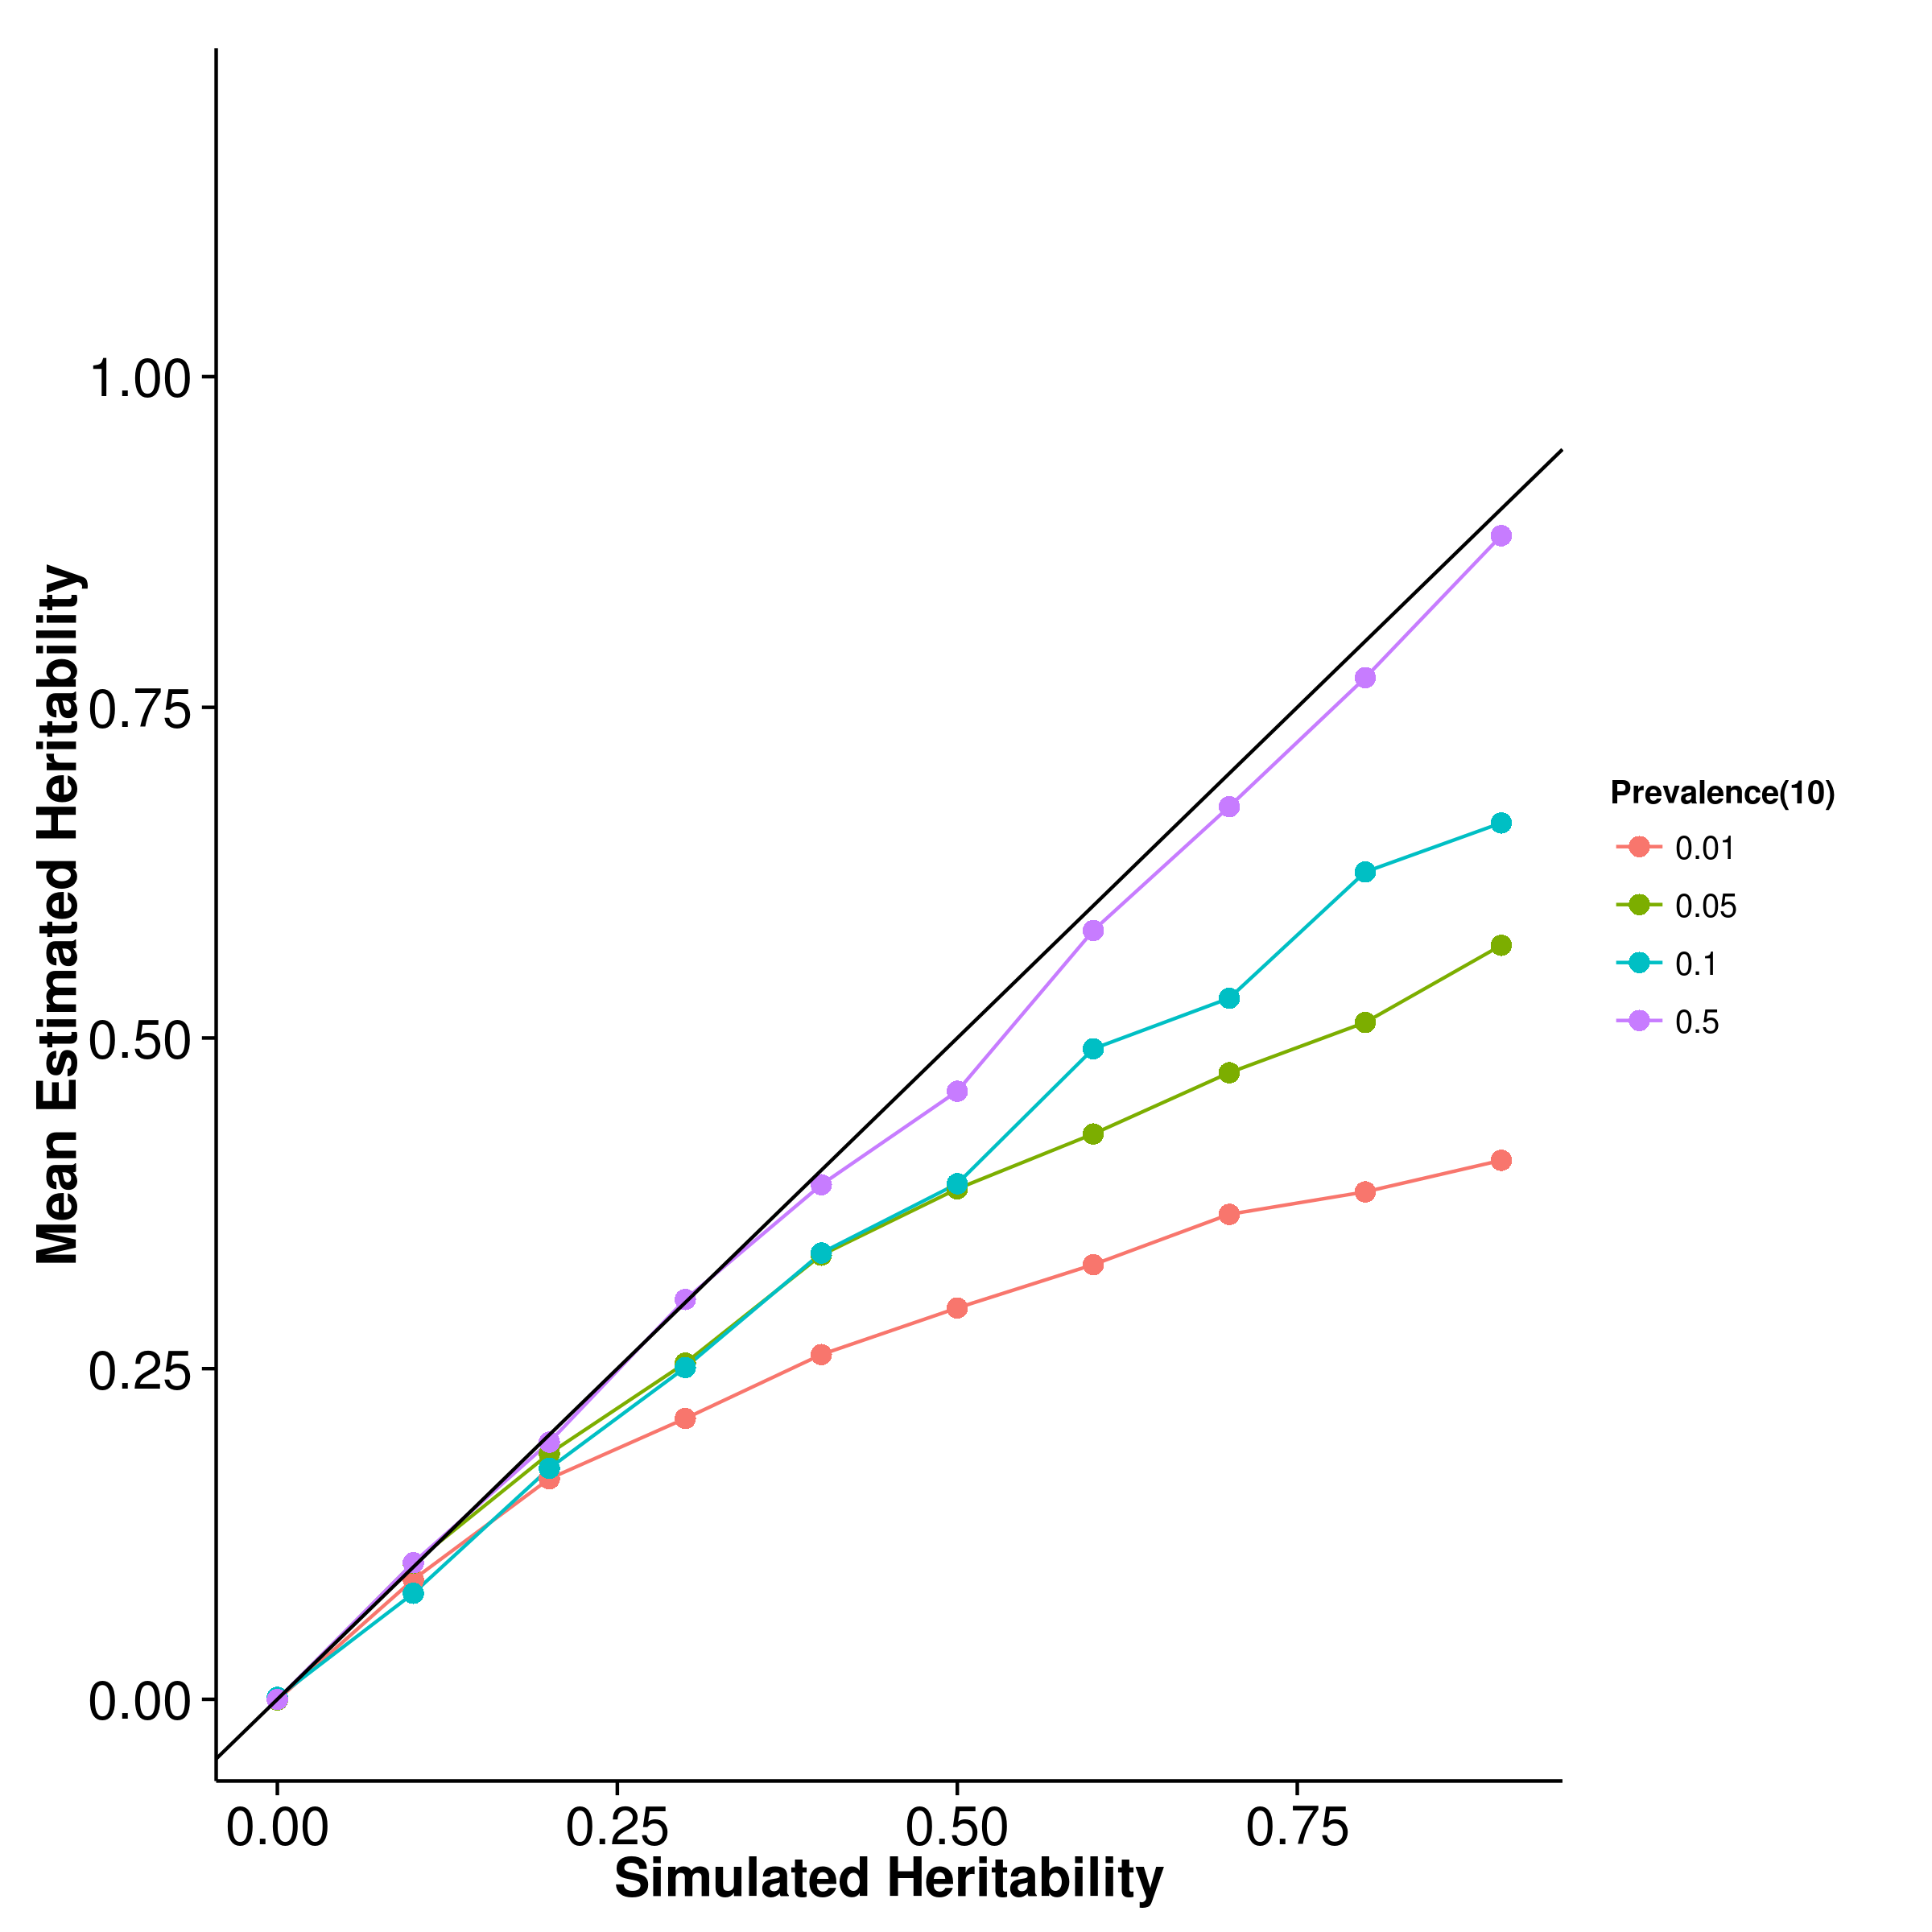
\includegraphics{figure/he_summary/cc_10c/gcta_CC_Rand_mean.png}}
		\label{fig:gctaCC10RandMean}
	}\\
	\subfloat[LDSC with fix intercept]{
		\scalebox{.4}{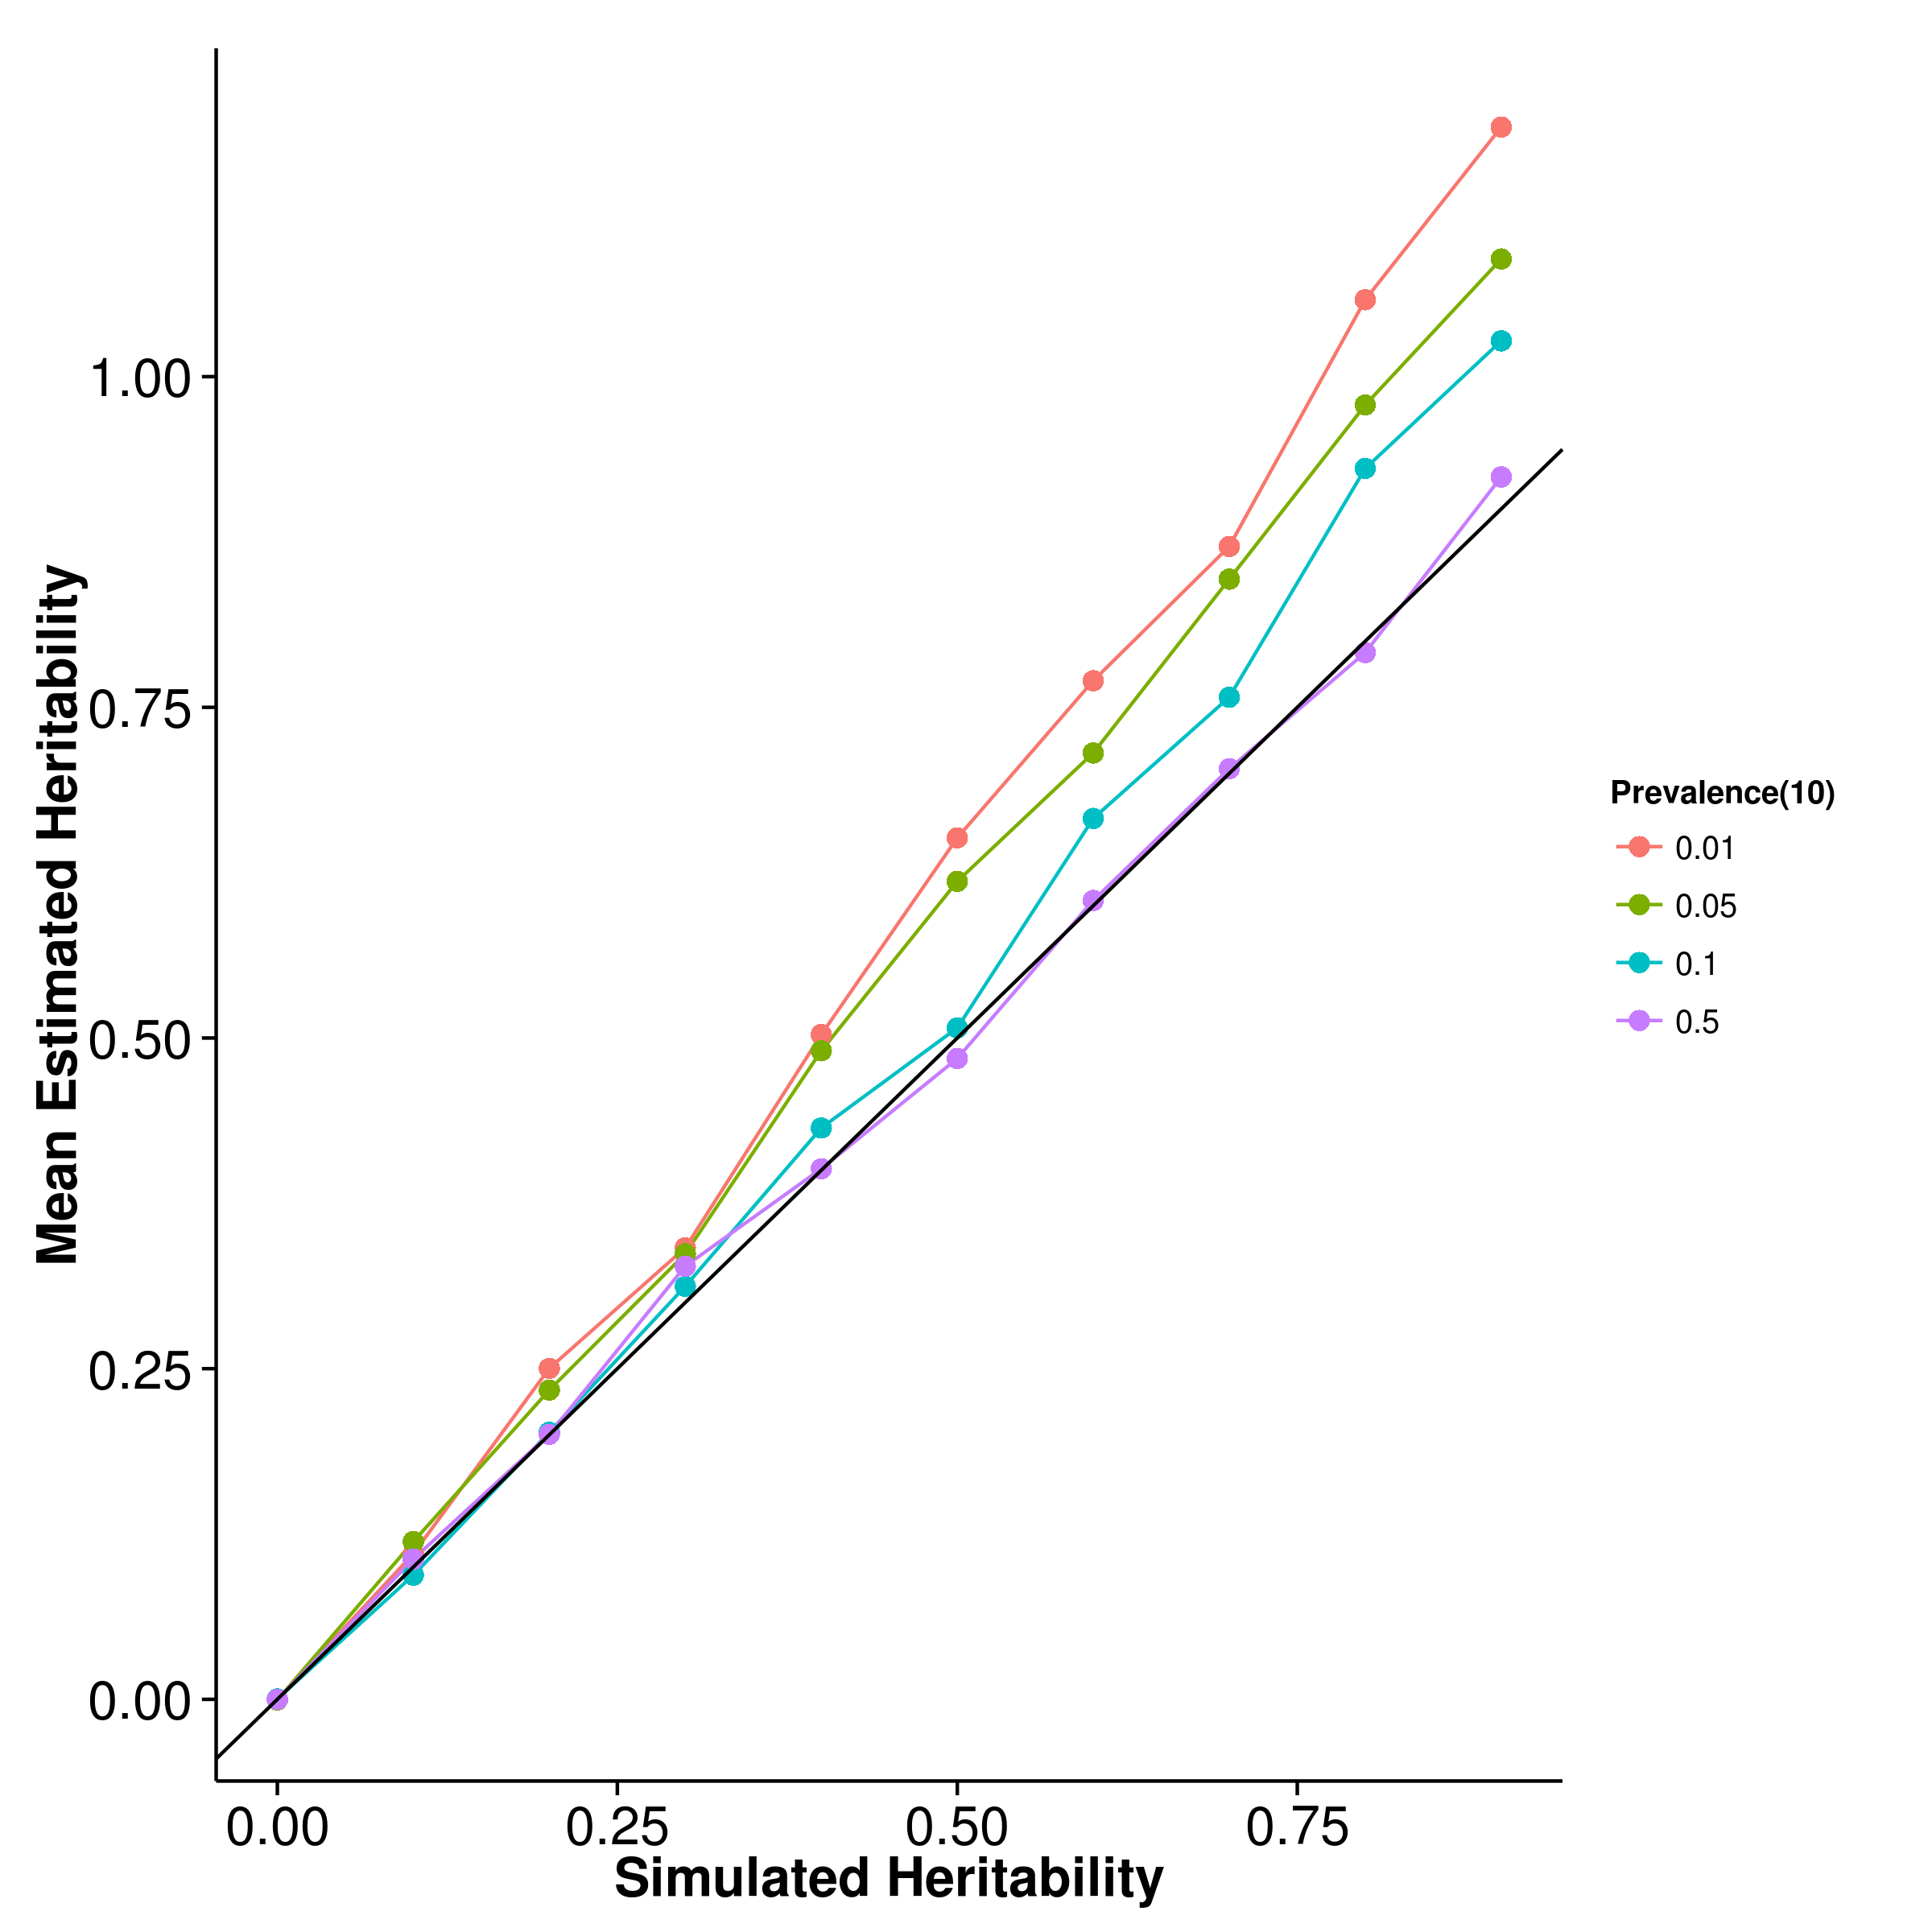
\includegraphics{figure/he_summary/cc_10c/ldsc_CC_Rand_mean.png}}
		\label{fig:ldscCC10RandMean}
	}
	\subfloat[LDSC with intercept estimation]{
		
		\scalebox{.4}{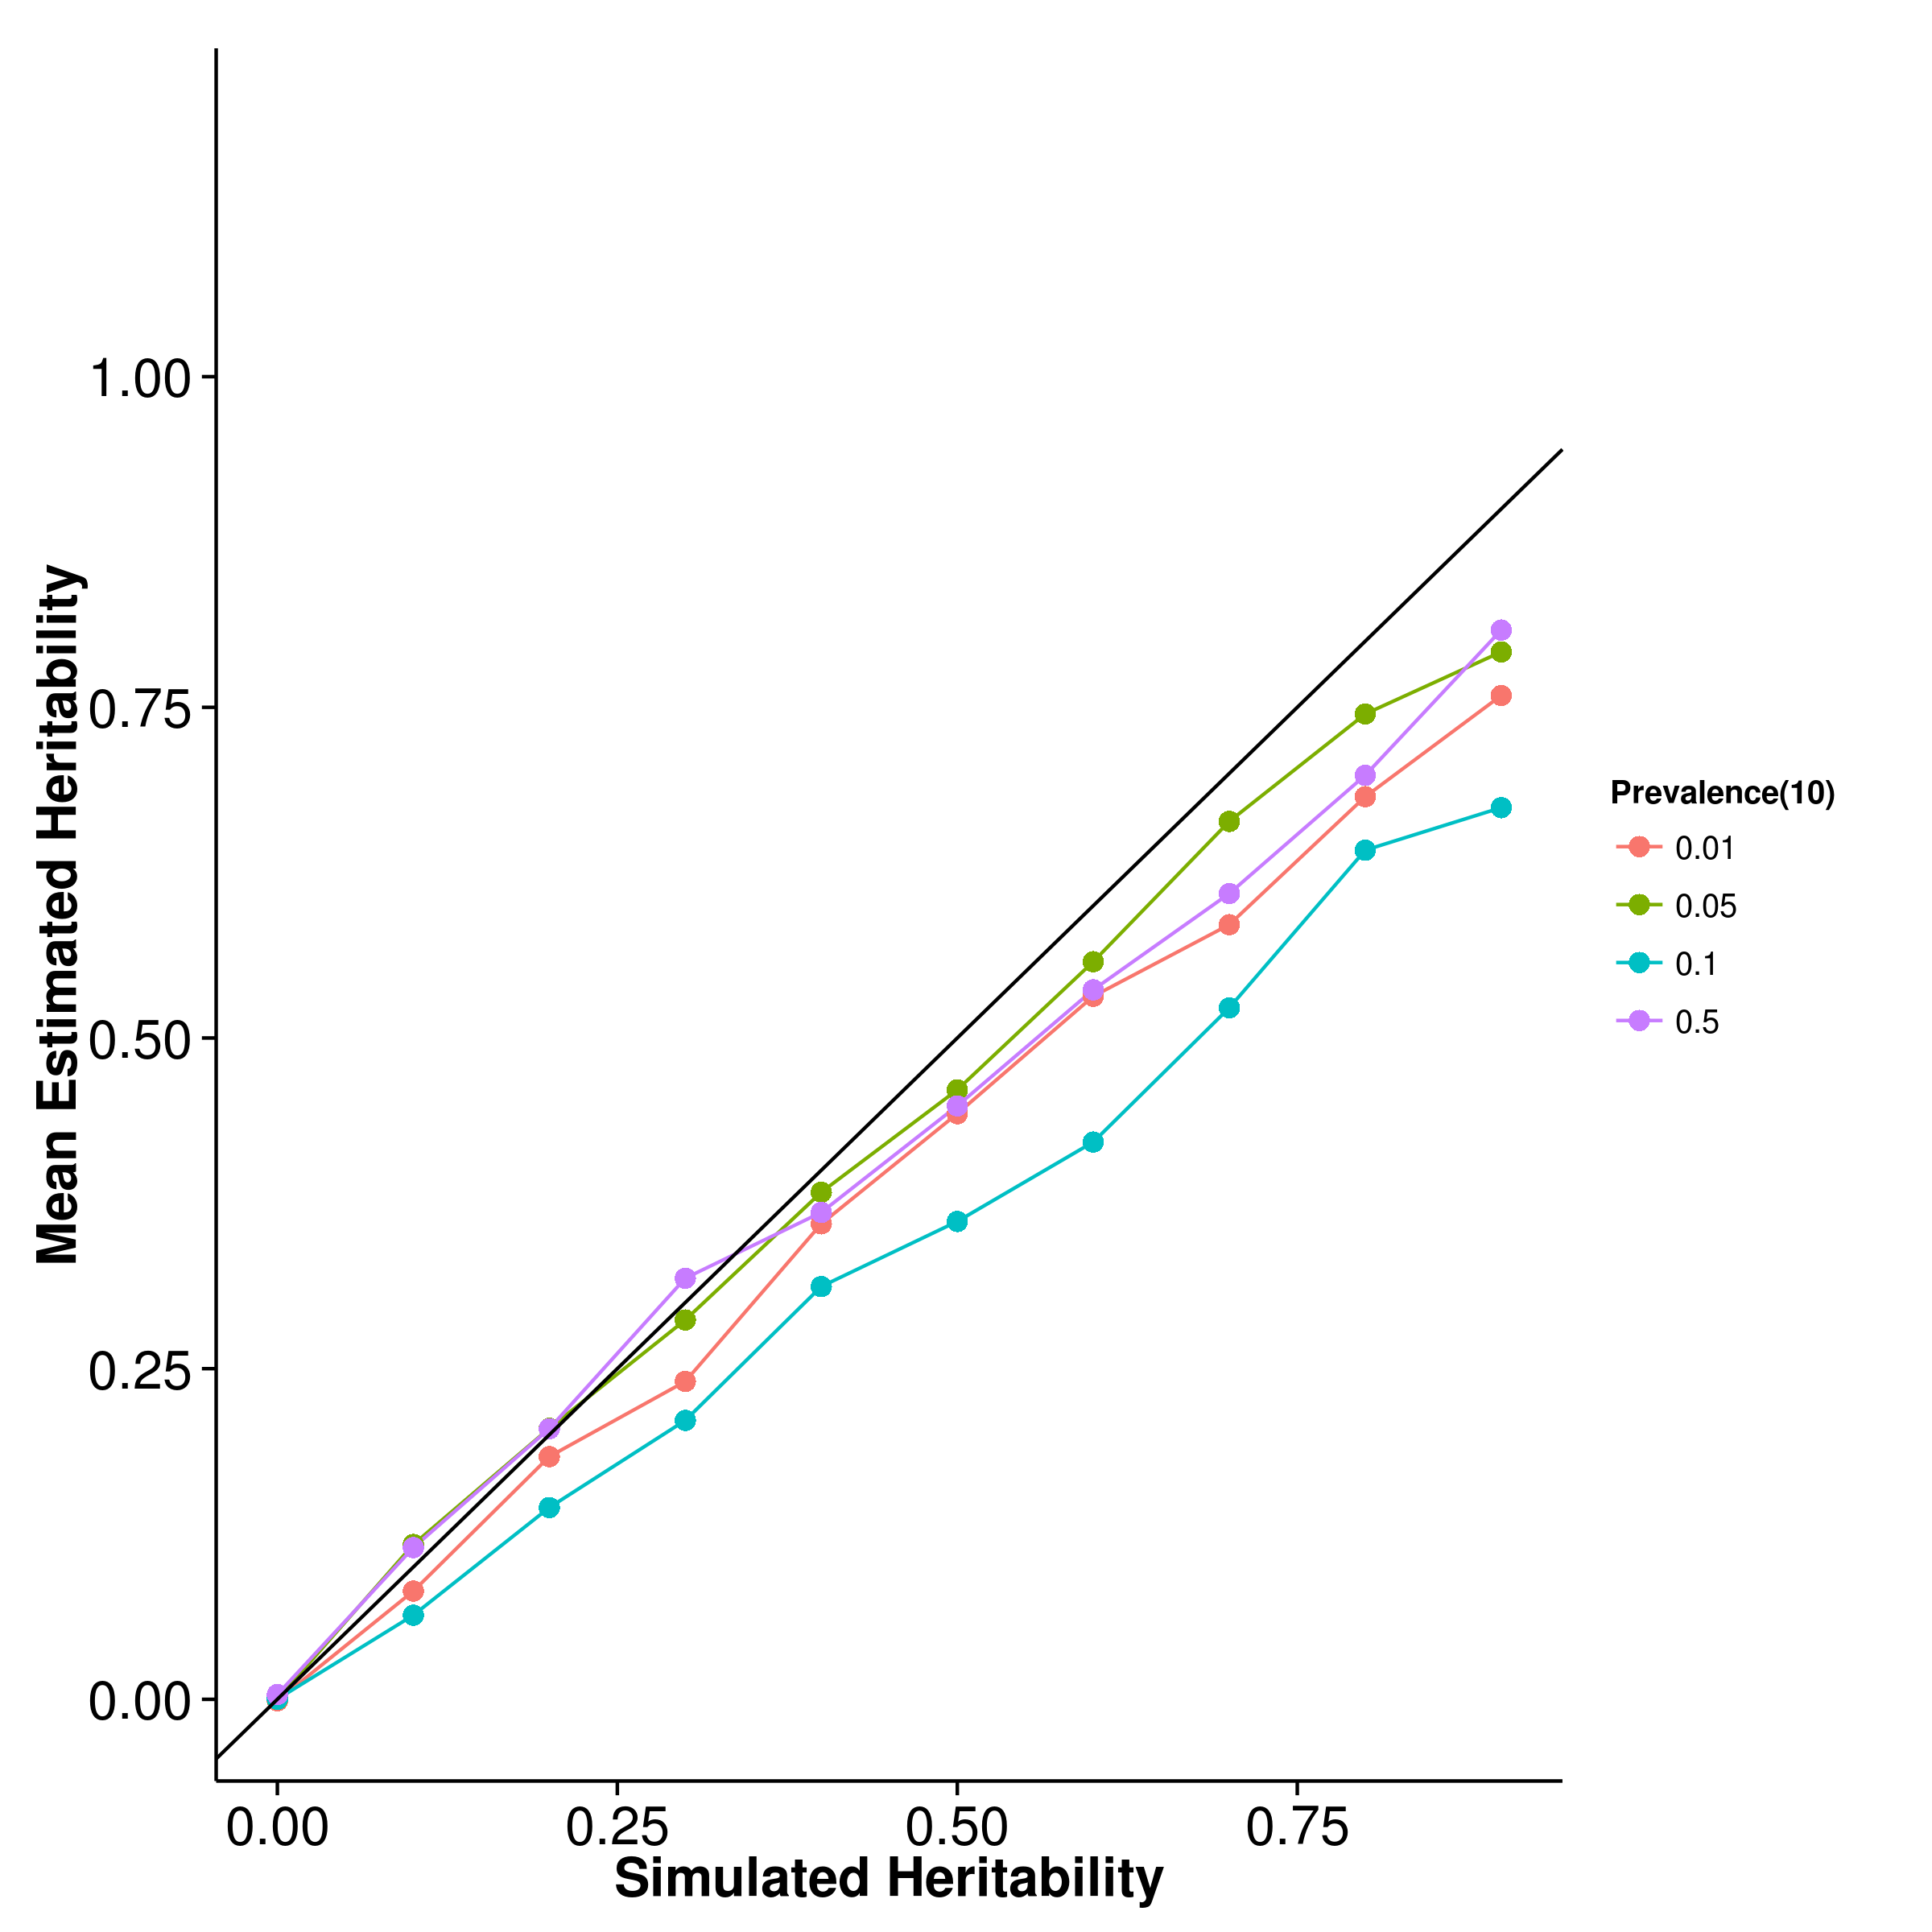
\includegraphics{figure/he_summary/cc_10c/ldscIn_CC_Rand_mean.png}}
		\label{fig:ldscInCC10RandMean}
	}
	\caption[Mean of Binary Trait Simulation Results (10 Causal)]
	{Mean of results from binary trait simulation with random effect size simulation with 10 causal \glspl{SNP}.
		The performance of \gls{gcta} was as suggested by \citet{Golan2014} where there was an underestimation as prevalence decreases.
		On the other hand, the upward bias of both \gls{ldsc} with fixed intercept and \gls{shrek} increases as the prevalence decreases whereas \gls{ldsc} with intercept estimation seems relatively robust to the change in prevalence.
	} 
	\label{fig:CC10RandMean}
\end{figure}
%Empirical Variance
\begin{figure}
	\centering
	\subfloat[SHREK]{
		\scalebox{.4}{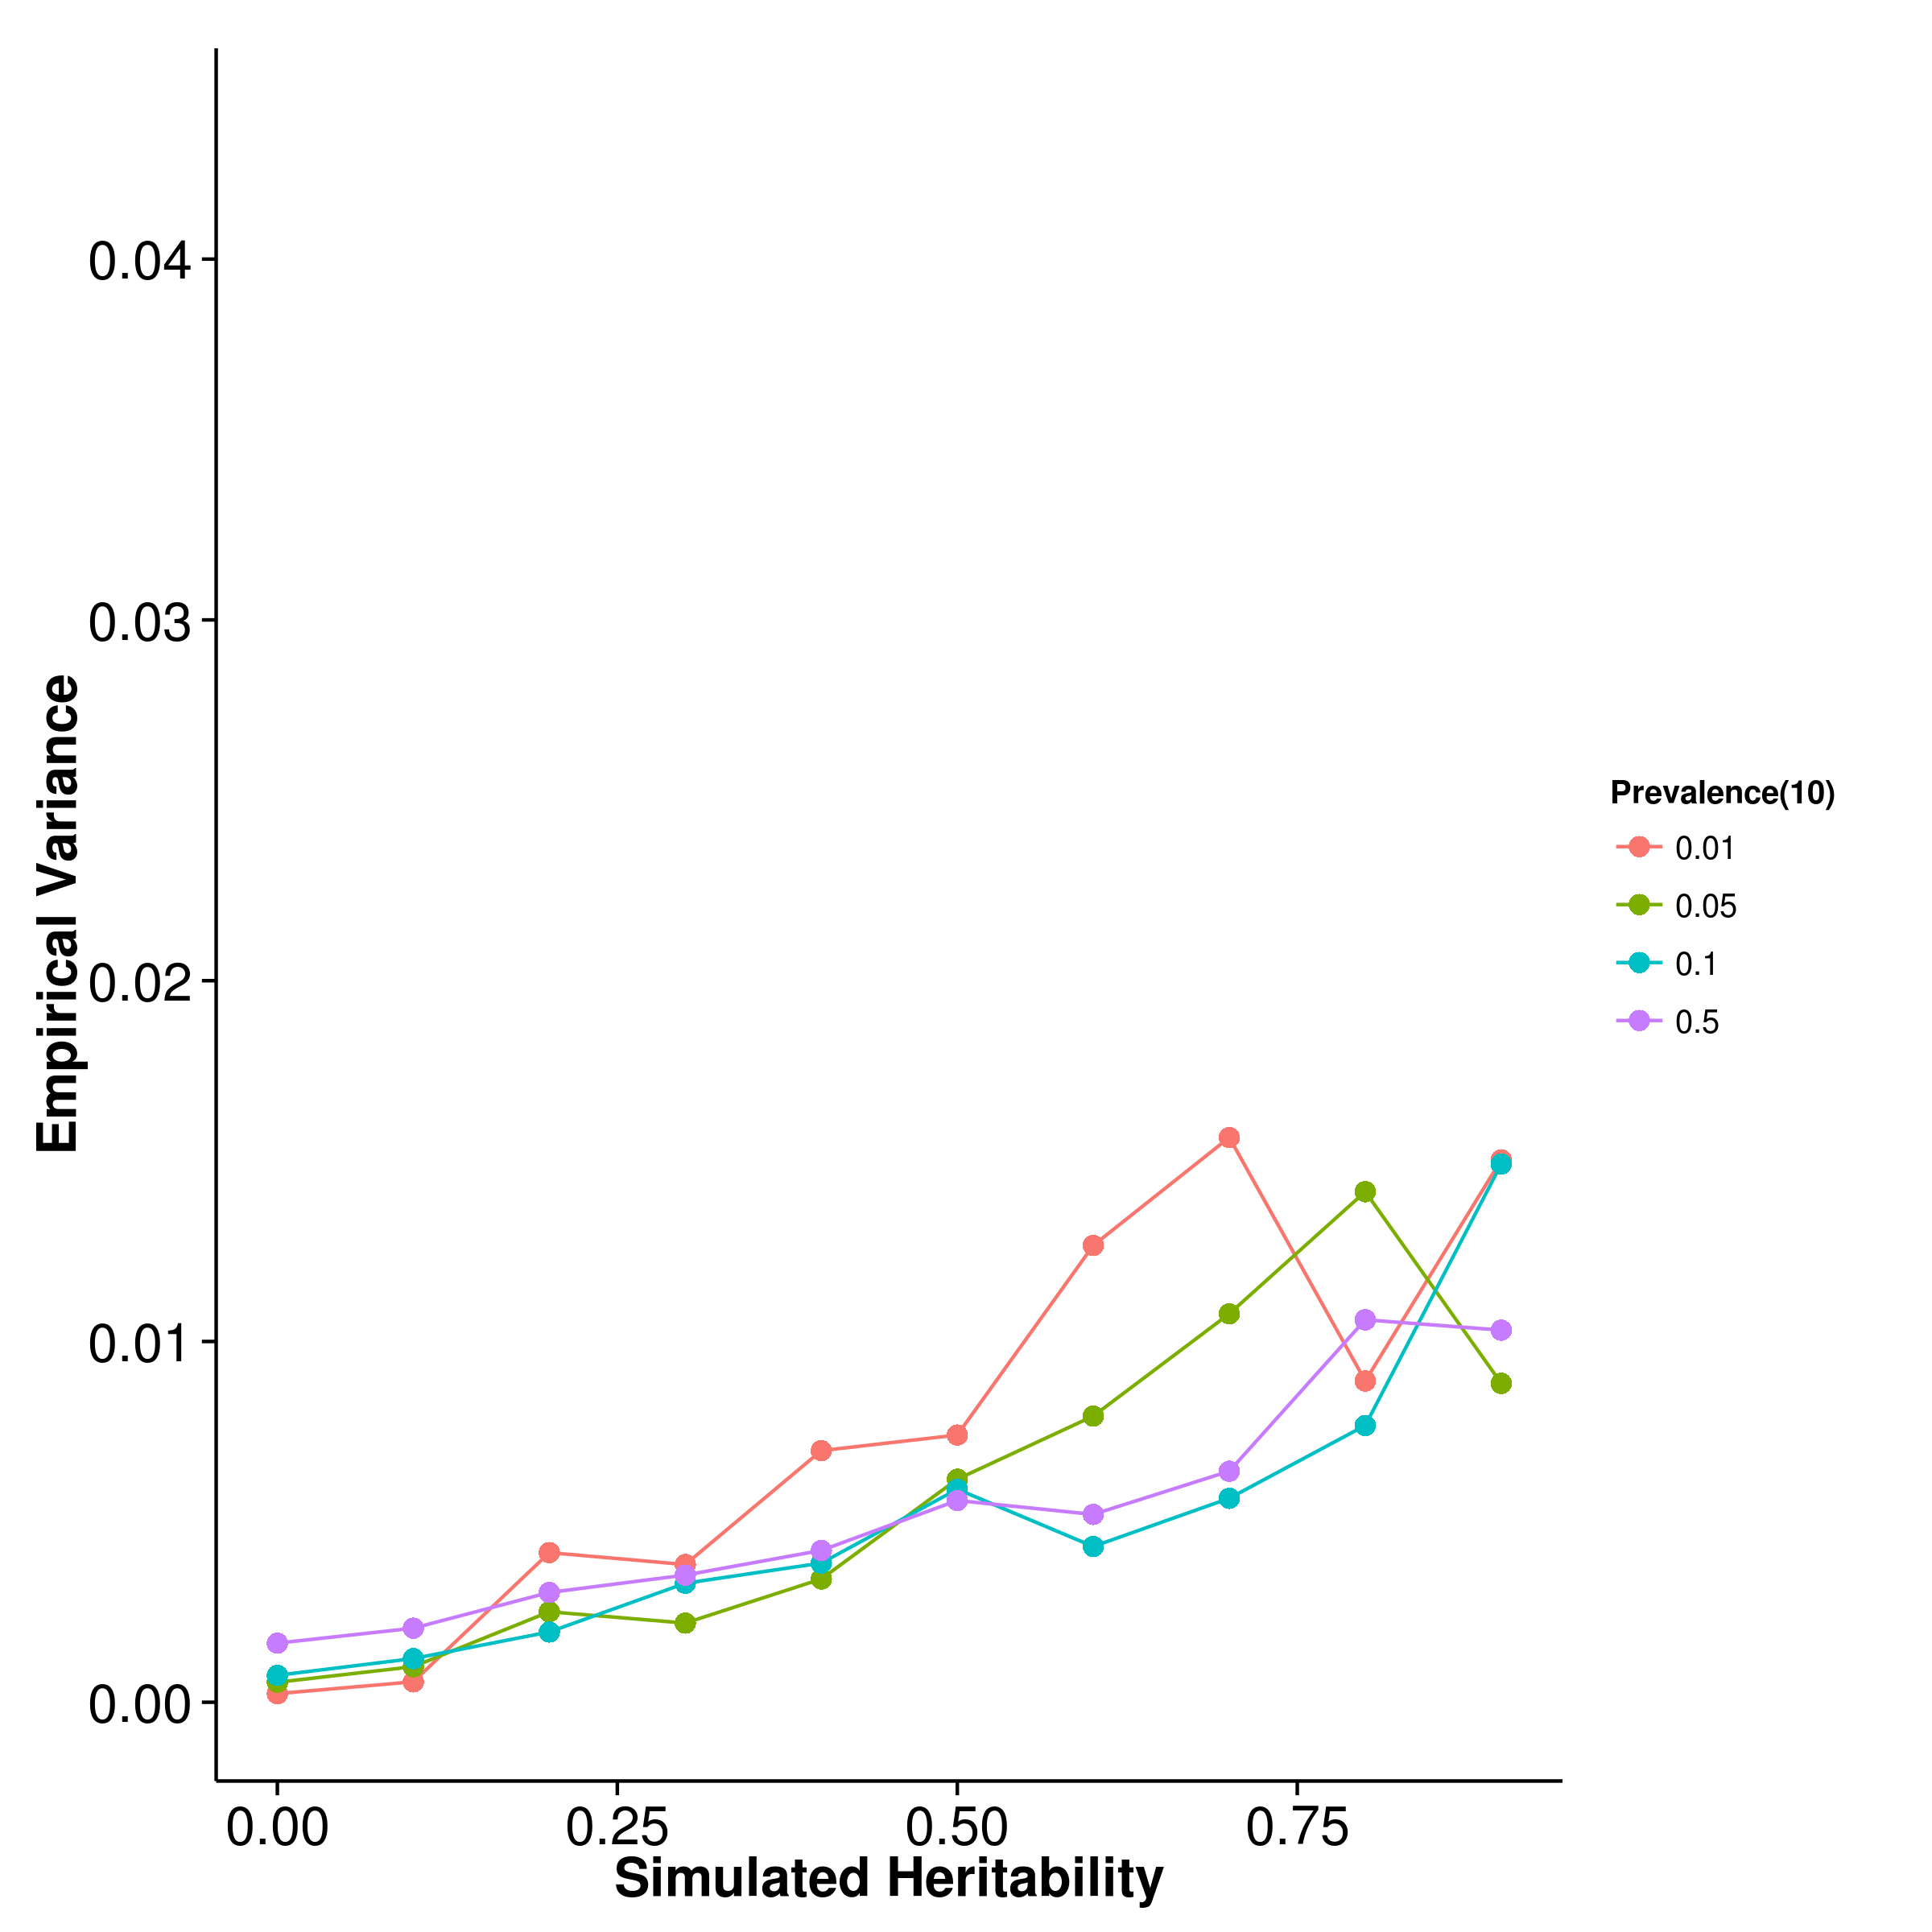
\includegraphics{figure/he_summary/cc_10c/shrek_CC_Rand_sd.png}}
		\label{fig:shrekCC10RandVar}
	}
	\subfloat[GCTA]{
		\scalebox{.4}{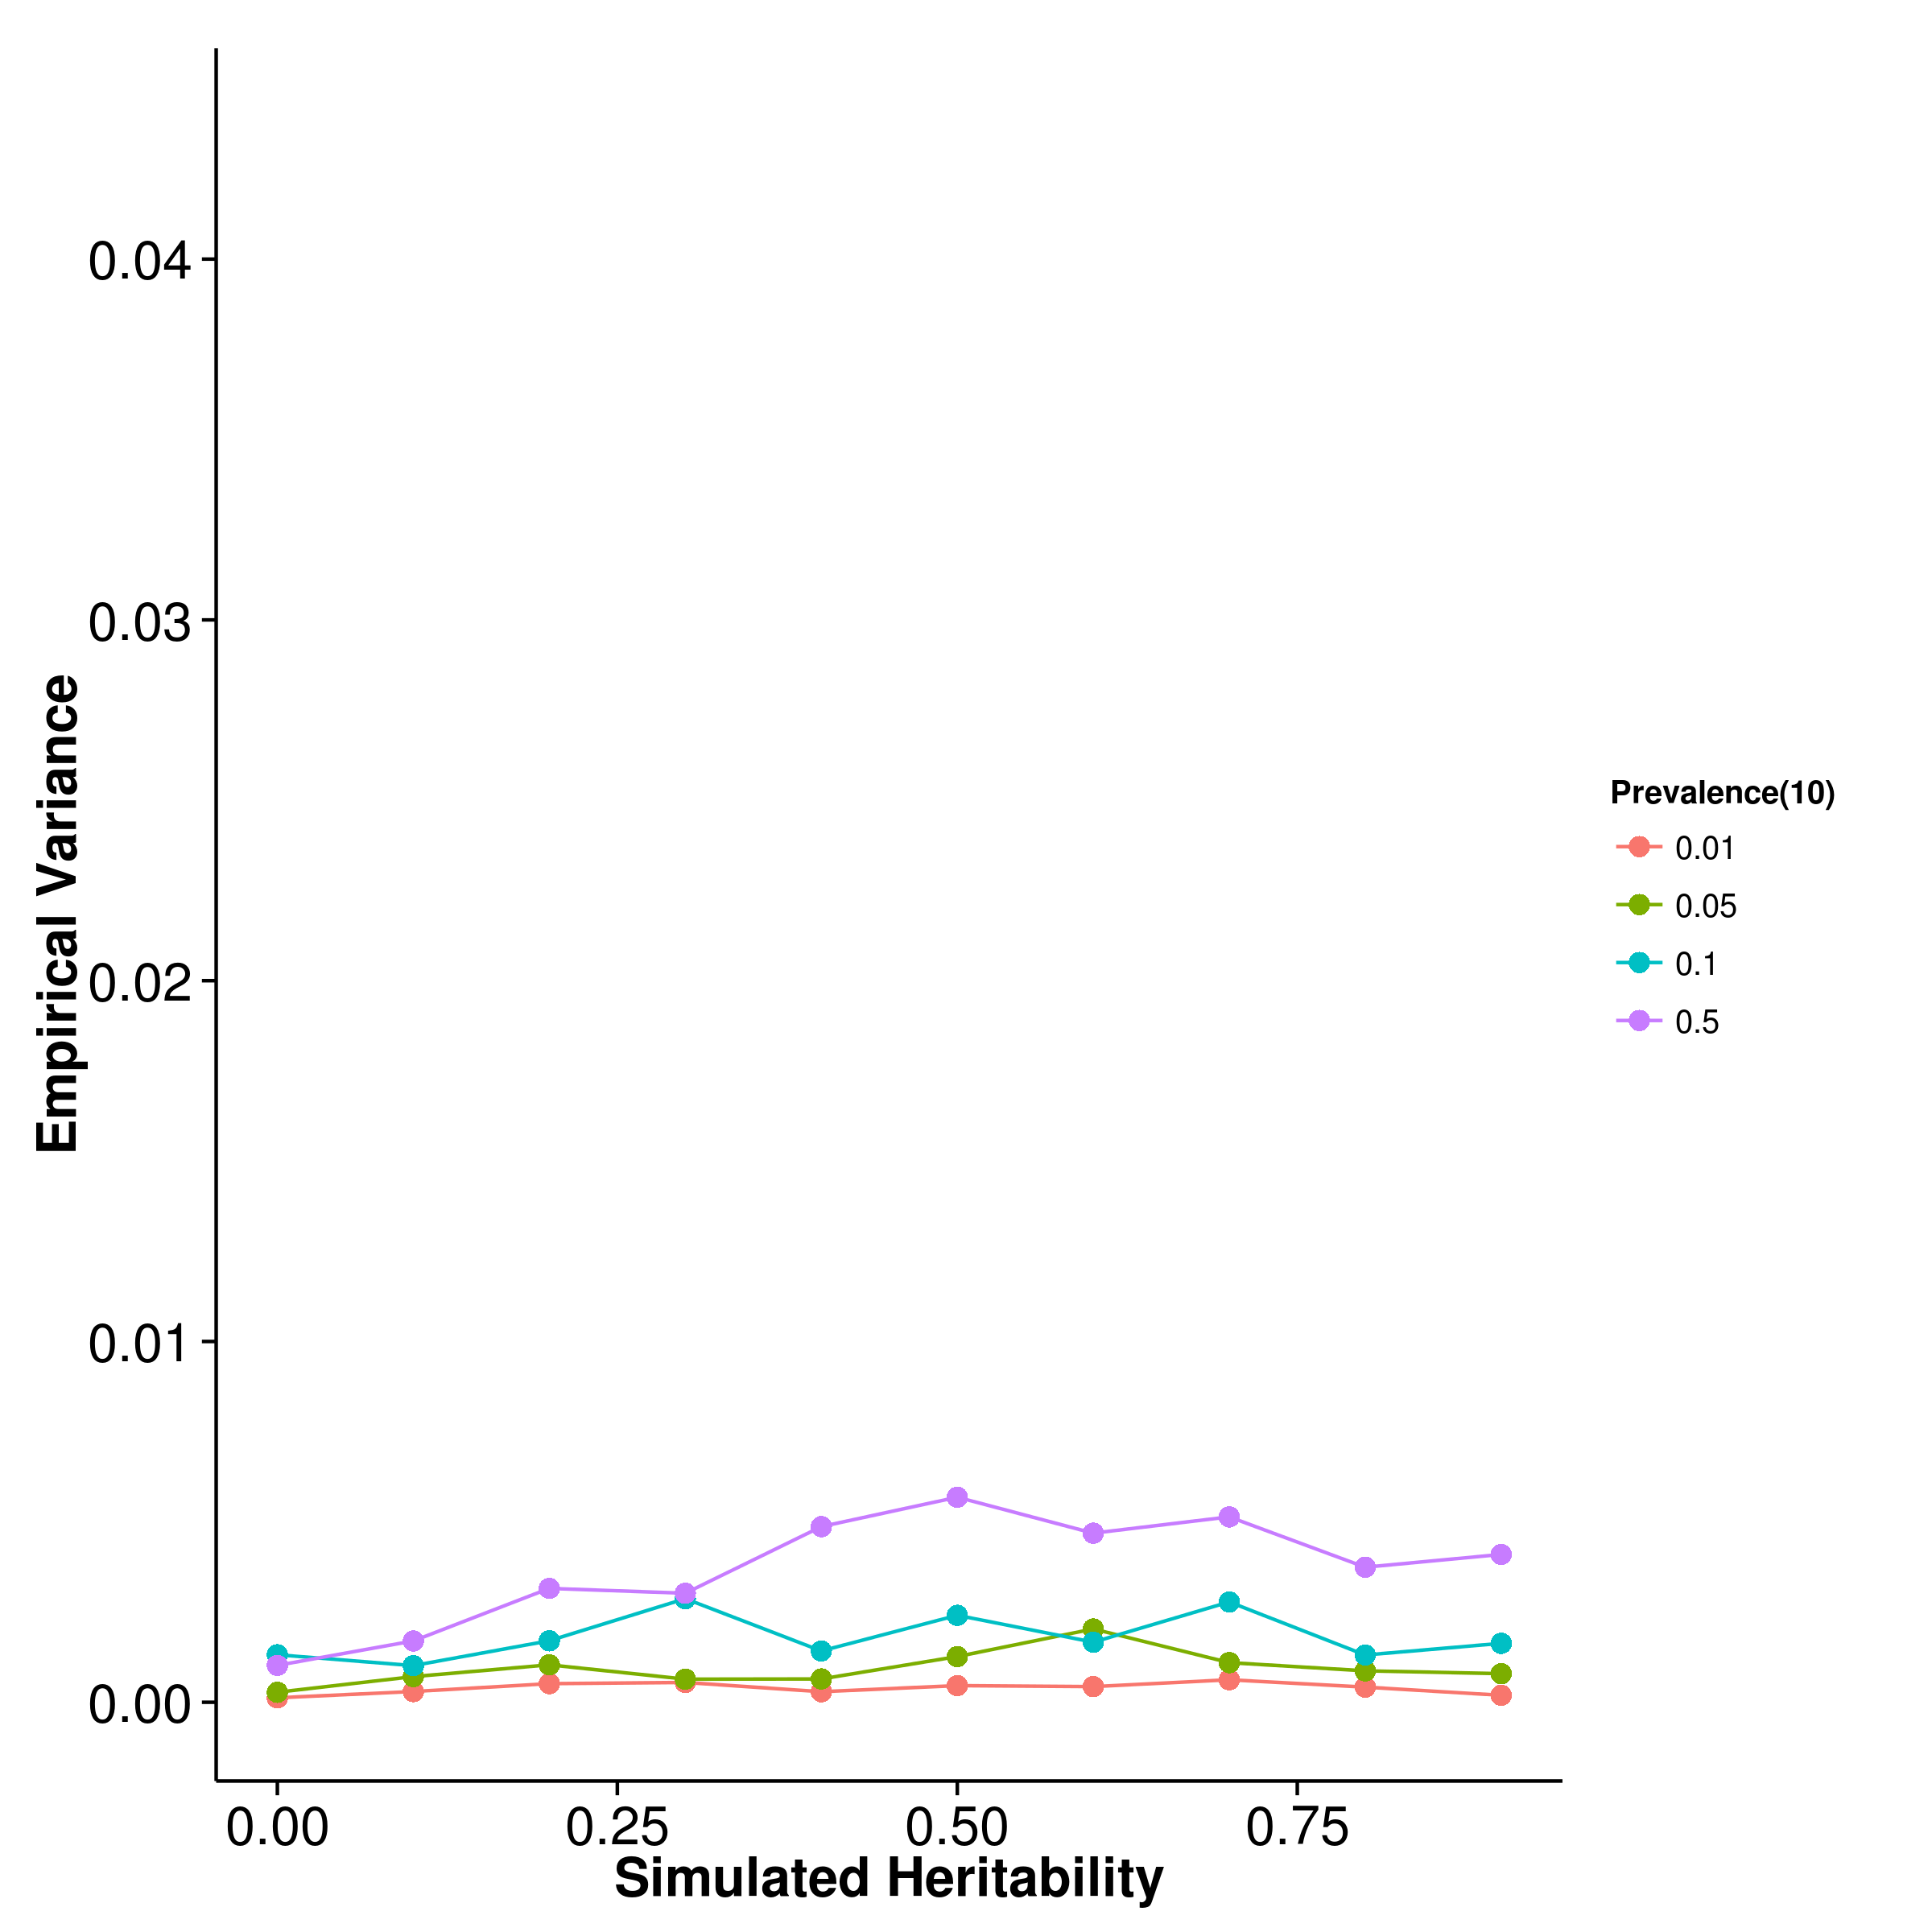
\includegraphics{figure/he_summary/cc_10c/gcta_CC_Rand_sd.png}}
		\label{fig:gctaCC10RandVar}
	}\\
	\subfloat[LDSC with fix intercept]{
		\scalebox{.4}{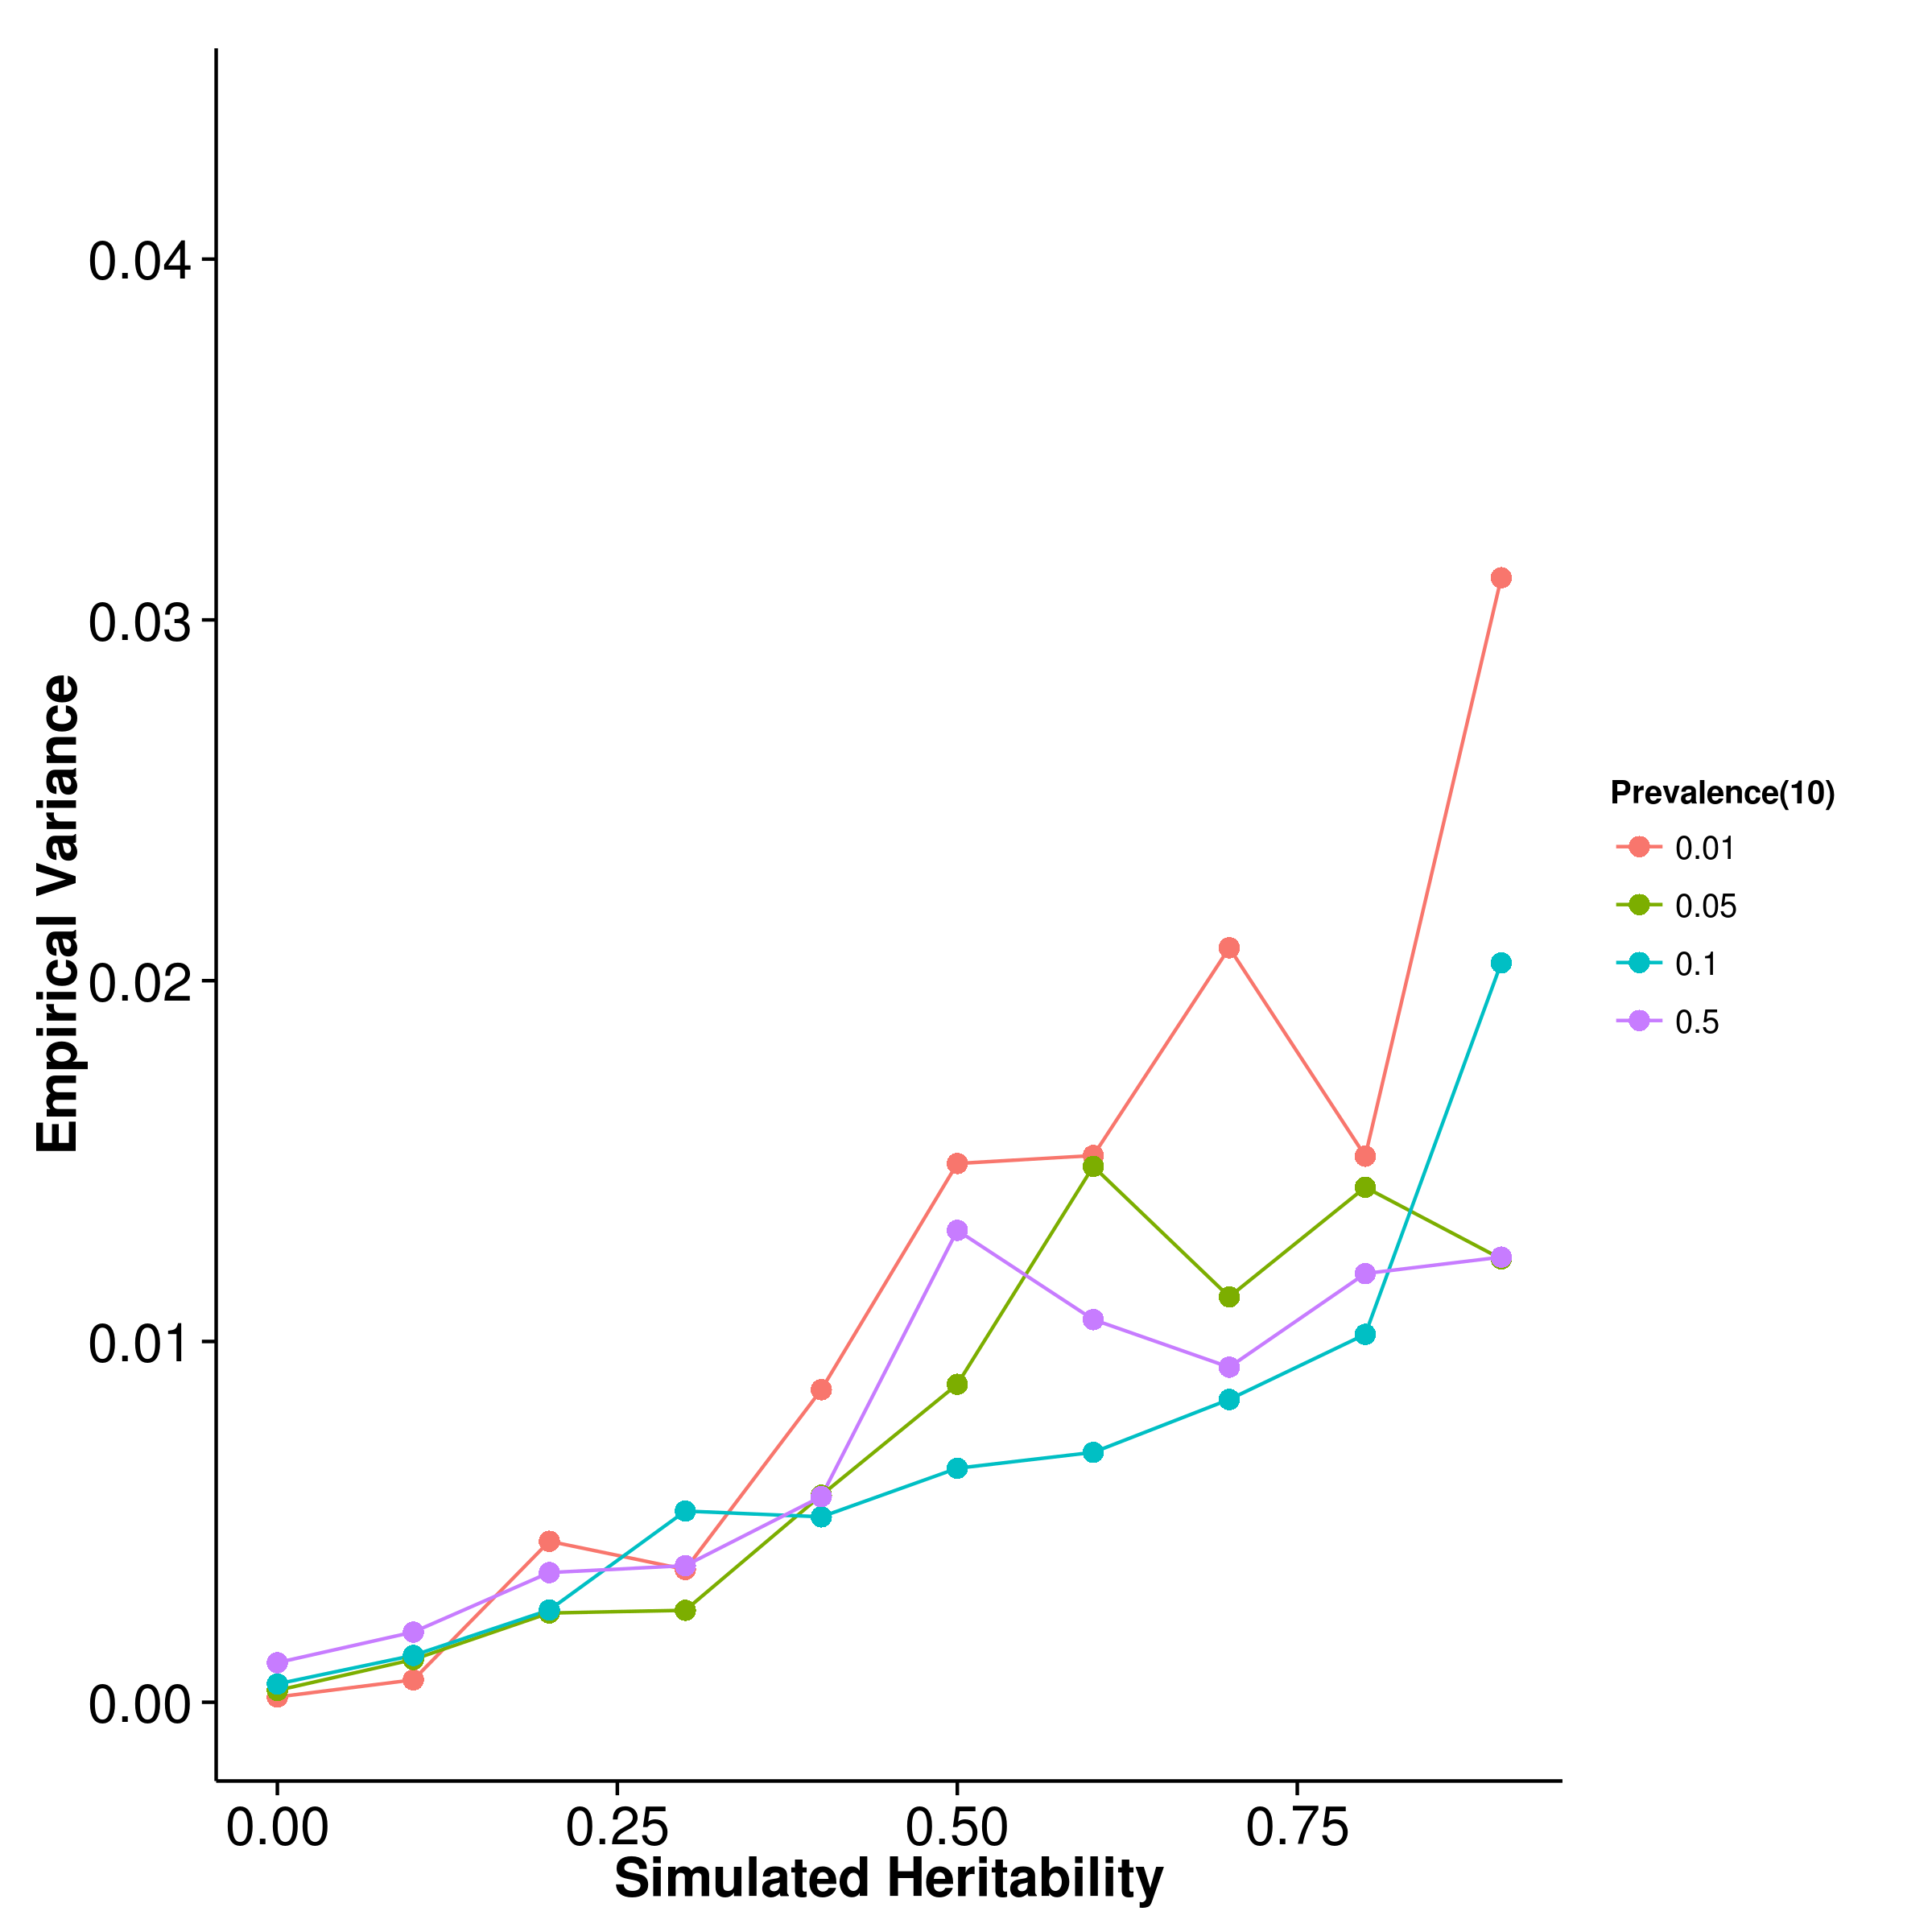
\includegraphics{figure/he_summary/cc_10c/ldsc_CC_Rand_sd.png}}
		\label{fig:ldscCC10RandVar}
	}
	\subfloat[LDSC with intercept estimation]{
		
		\scalebox{.4}{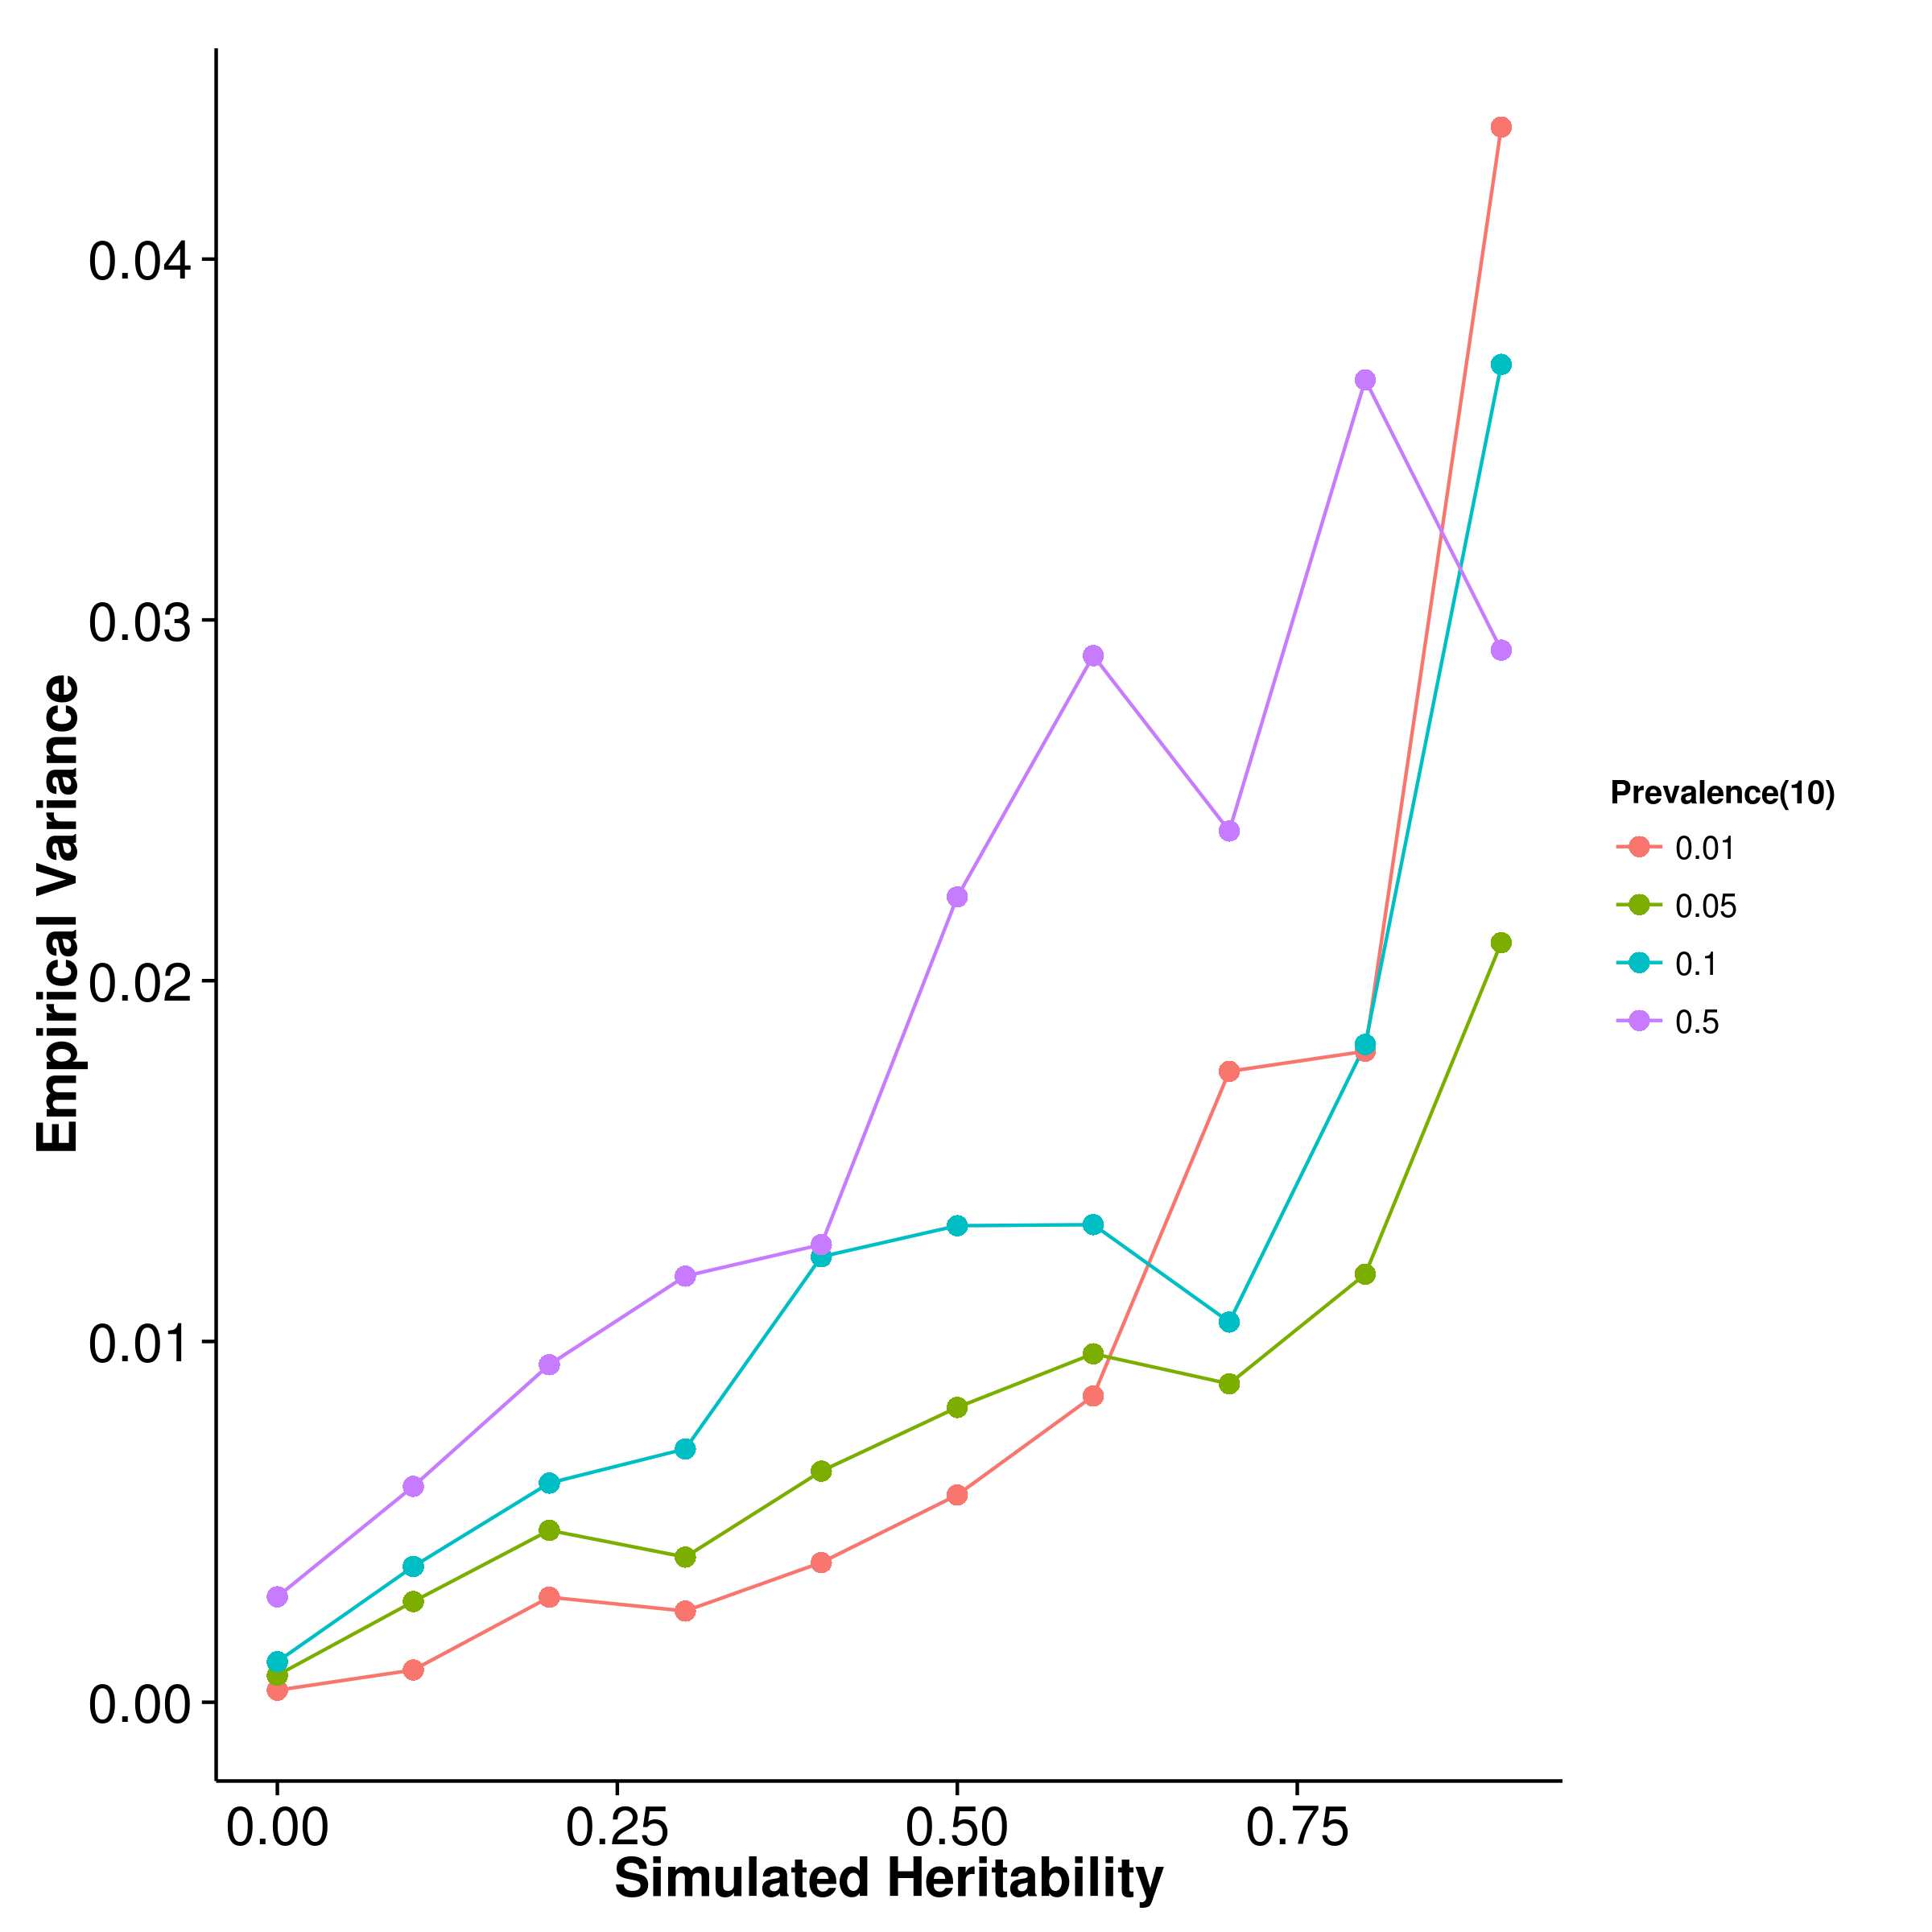
\includegraphics{figure/he_summary/cc_10c/ldscIn_CC_Rand_sd.png}}
		\label{fig:ldscInCC10RandVar}
	}
	\caption[Variance of Binary Trait Simulation Results (10 Causal)]
	{Variance of results from binary trait simulation with random effect size simulation with 10 causal \glspl{SNP}.
		There were no clear pattern as to how the prevalence affect the empirical variance of estimates from \gls{shrek} and \gls{ldsc}. 
		For \gls{gcta}, it seems like a larger prevalence tends to result in a larger empirical variance. 
		Again, \gls{gcta} has the lowest variance, follow by \gls{shrek} and \gls{ldsc} with fixed intercept.
		Nonetheless, it was important to remember that in binary trait simulation, a much smaller amount of \glspl{SNP} was used, thus the results was not directly comparable to results from the quantitative simulation.
	} 
	\label{fig:CC10RandVar}
\end{figure}
%Variance estimation			
\begin{figure}
	\centering
	\subfloat[SHREK]{
		\scalebox{.4}{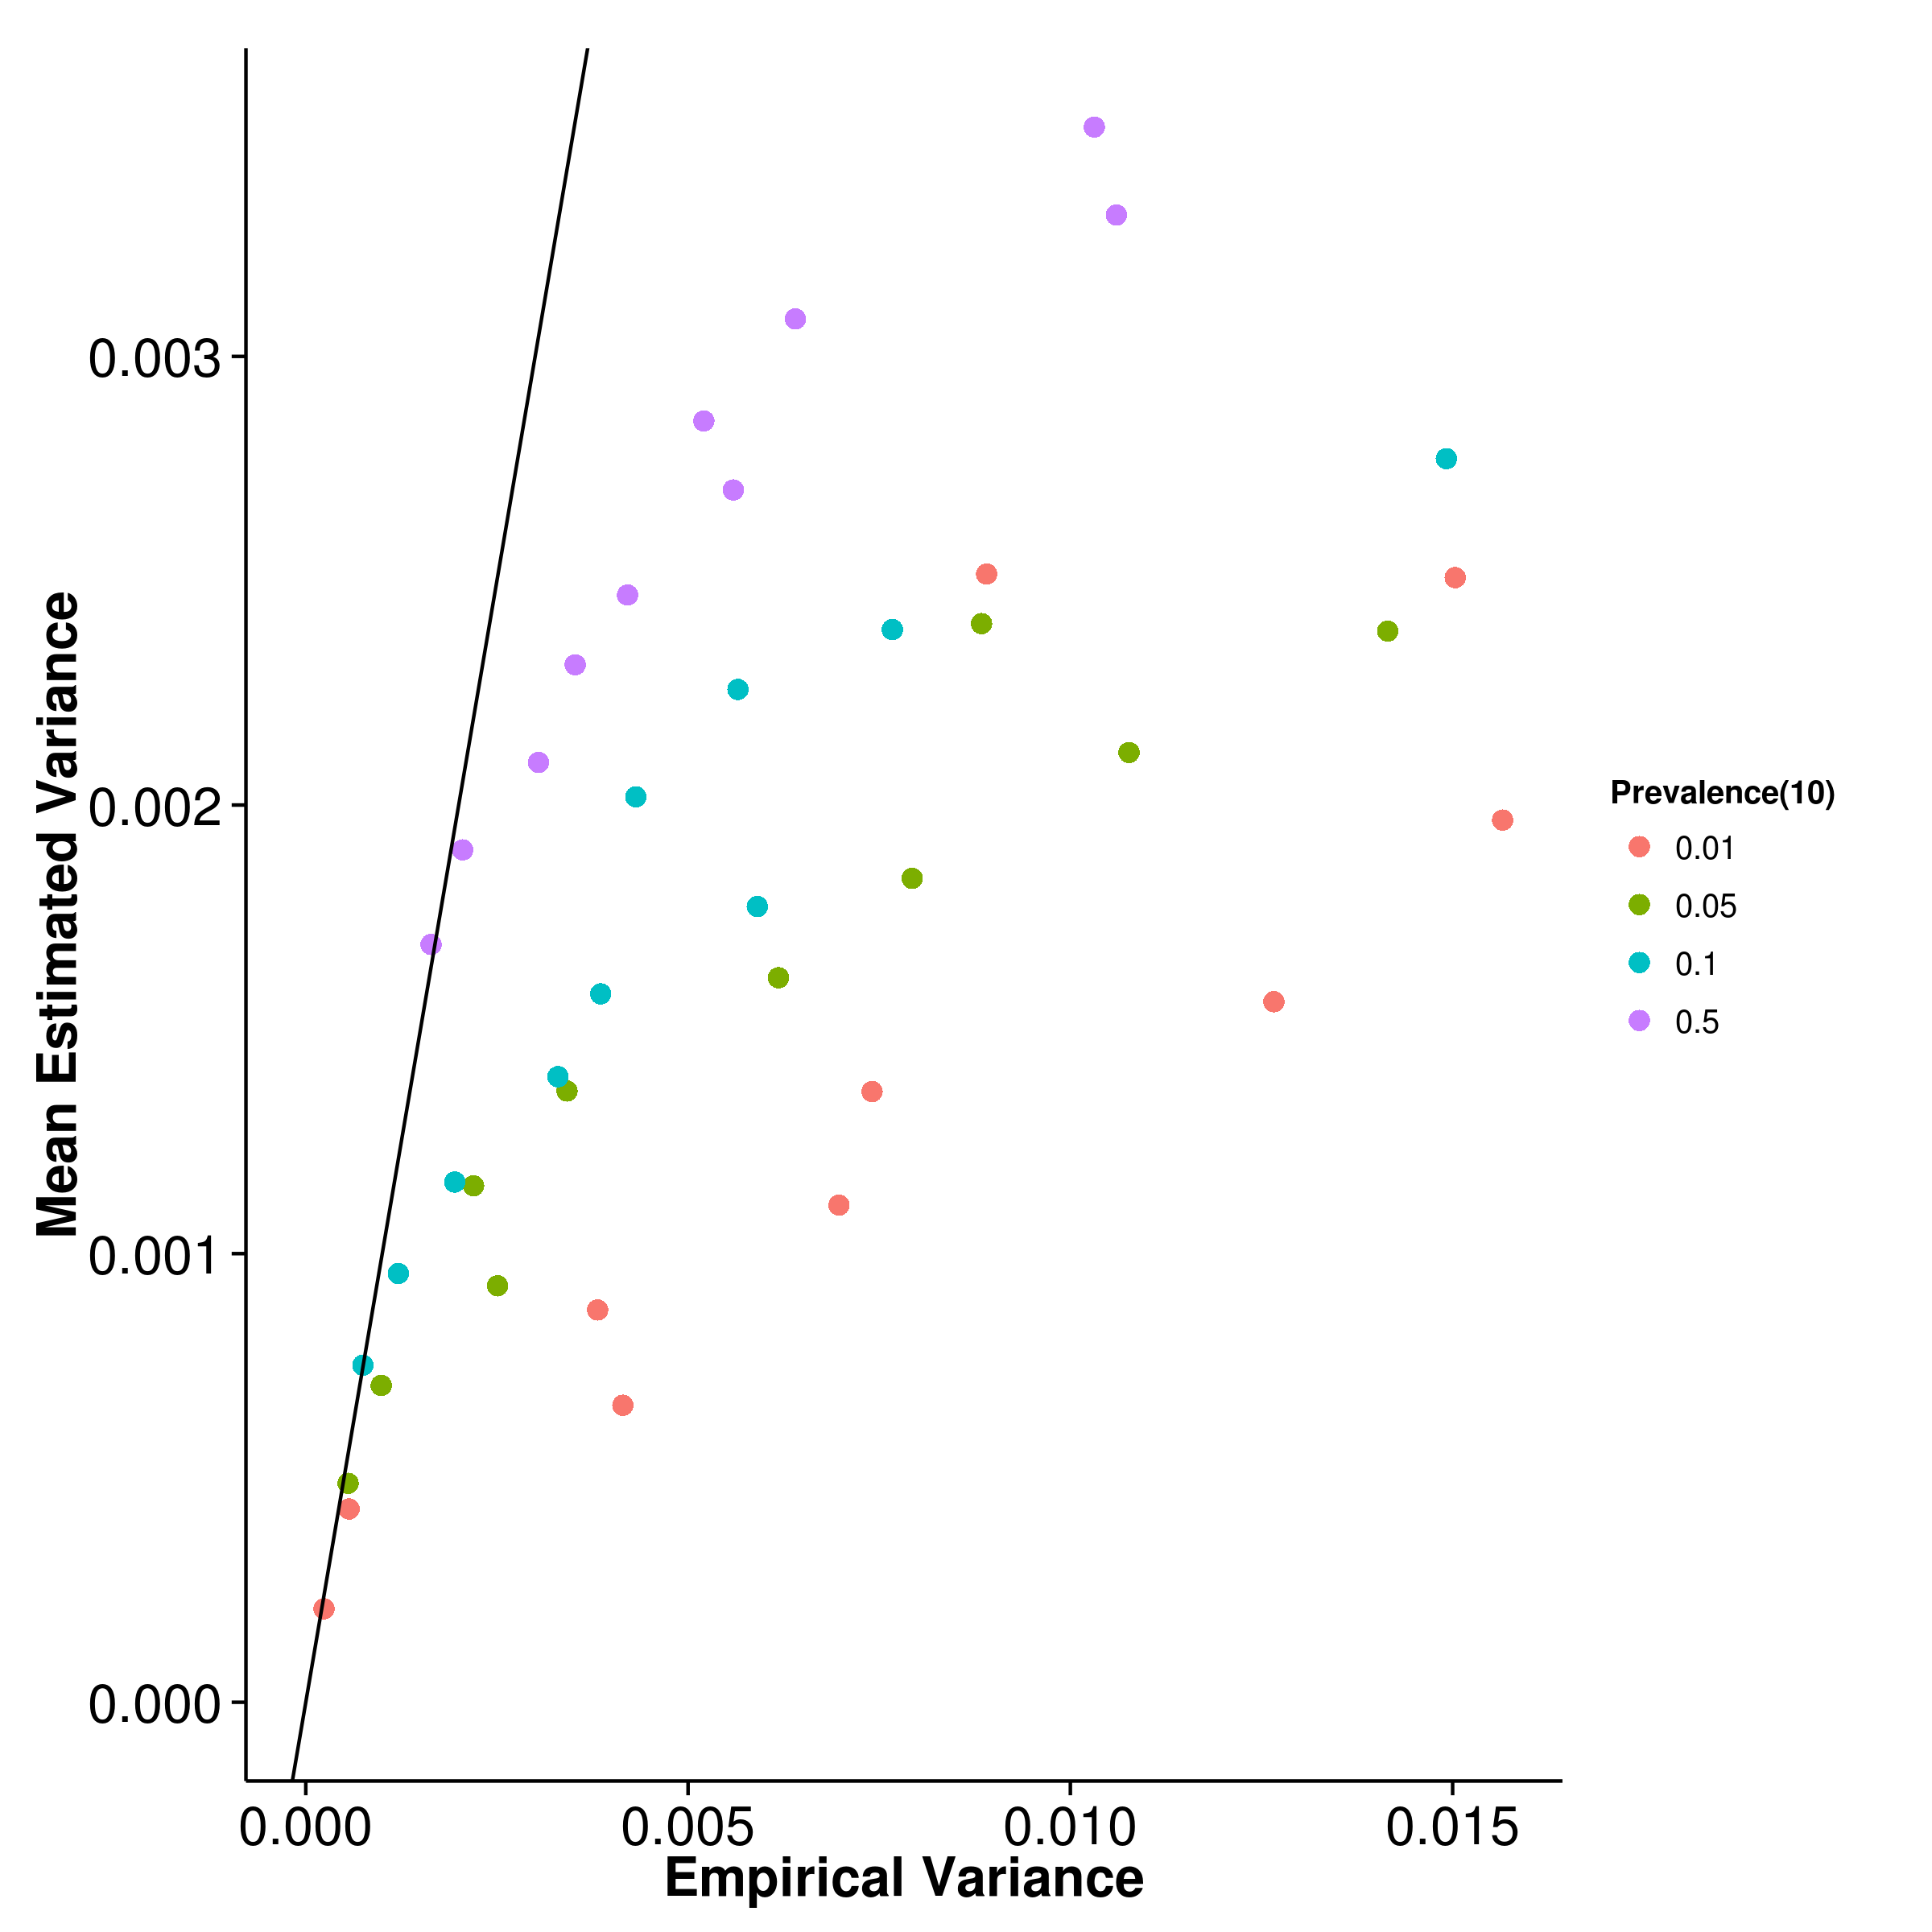
\includegraphics{figure/he_summary/cc_10c/shrek_CC_Rand_sdCom.png}}
		\label{fig:shrekCC10RandVarCom}
	}
	\subfloat[GCTA]{
		\scalebox{.4}{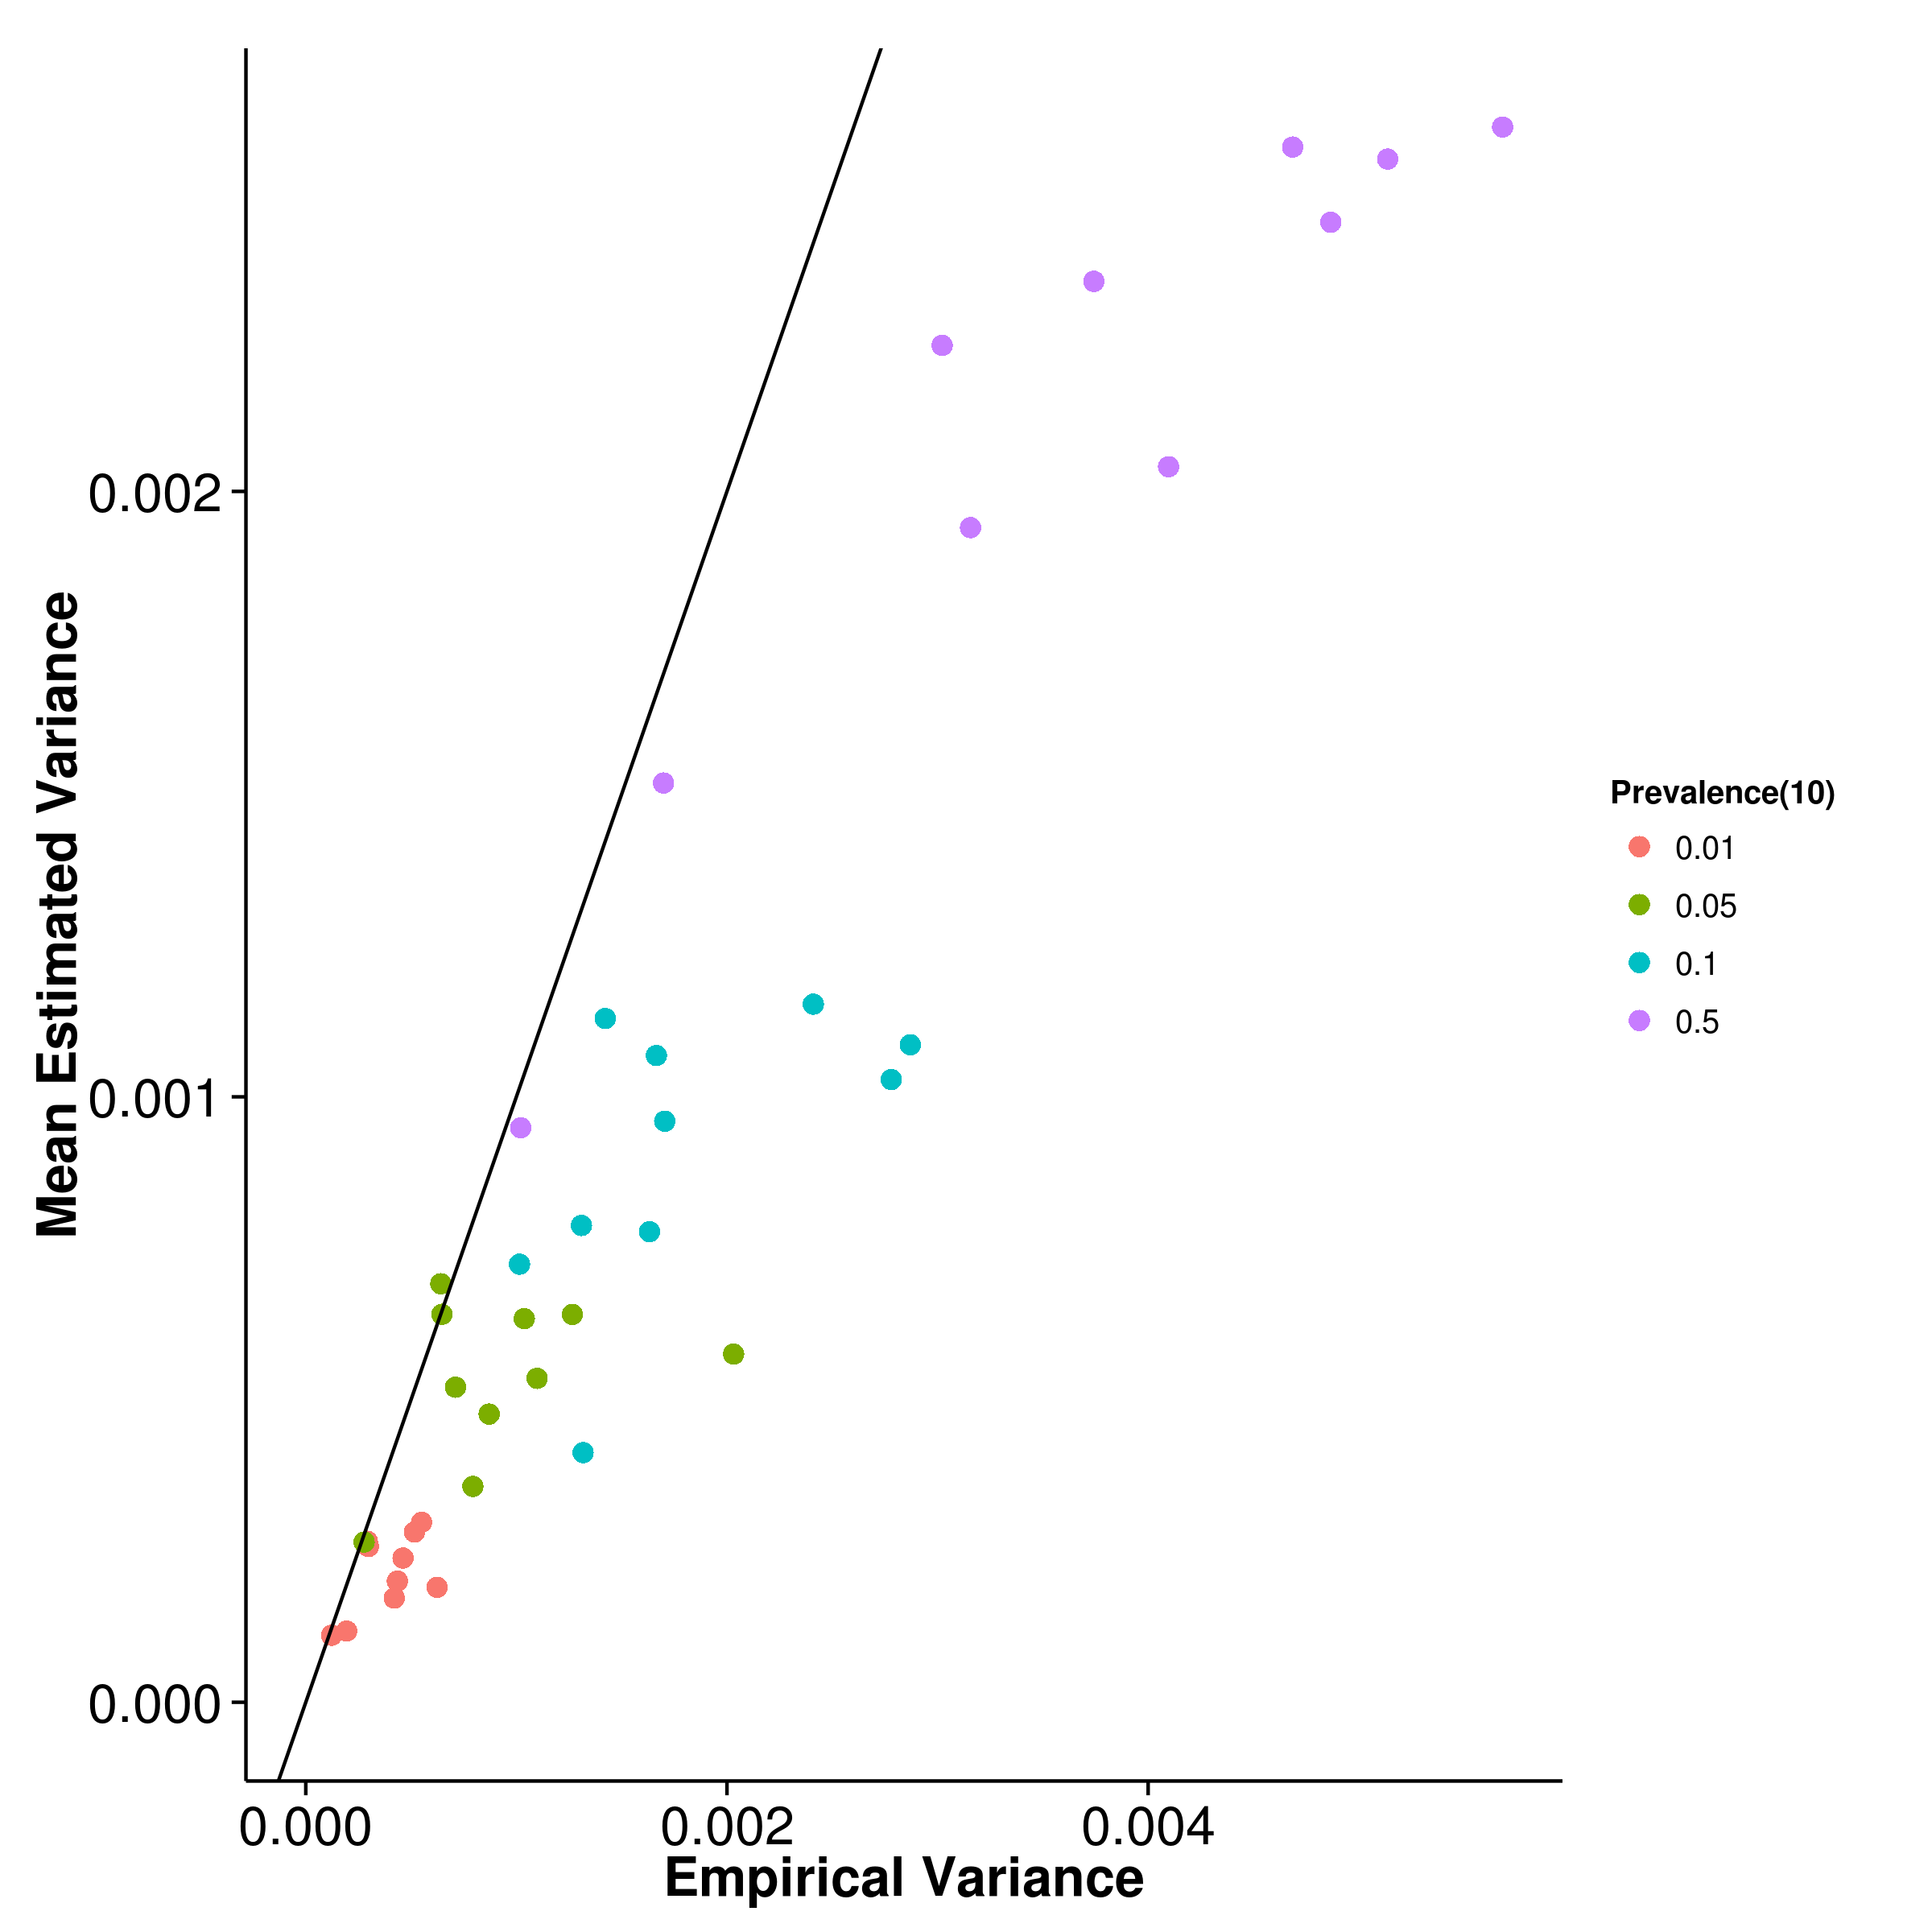
\includegraphics{figure/he_summary/cc_10c/gcta_CC_Rand_sdCom.png}}
		\label{fig:gctaCC10RandVarCom}
	}\\
	\subfloat[LDSC with fix intercept]{
		\scalebox{.4}{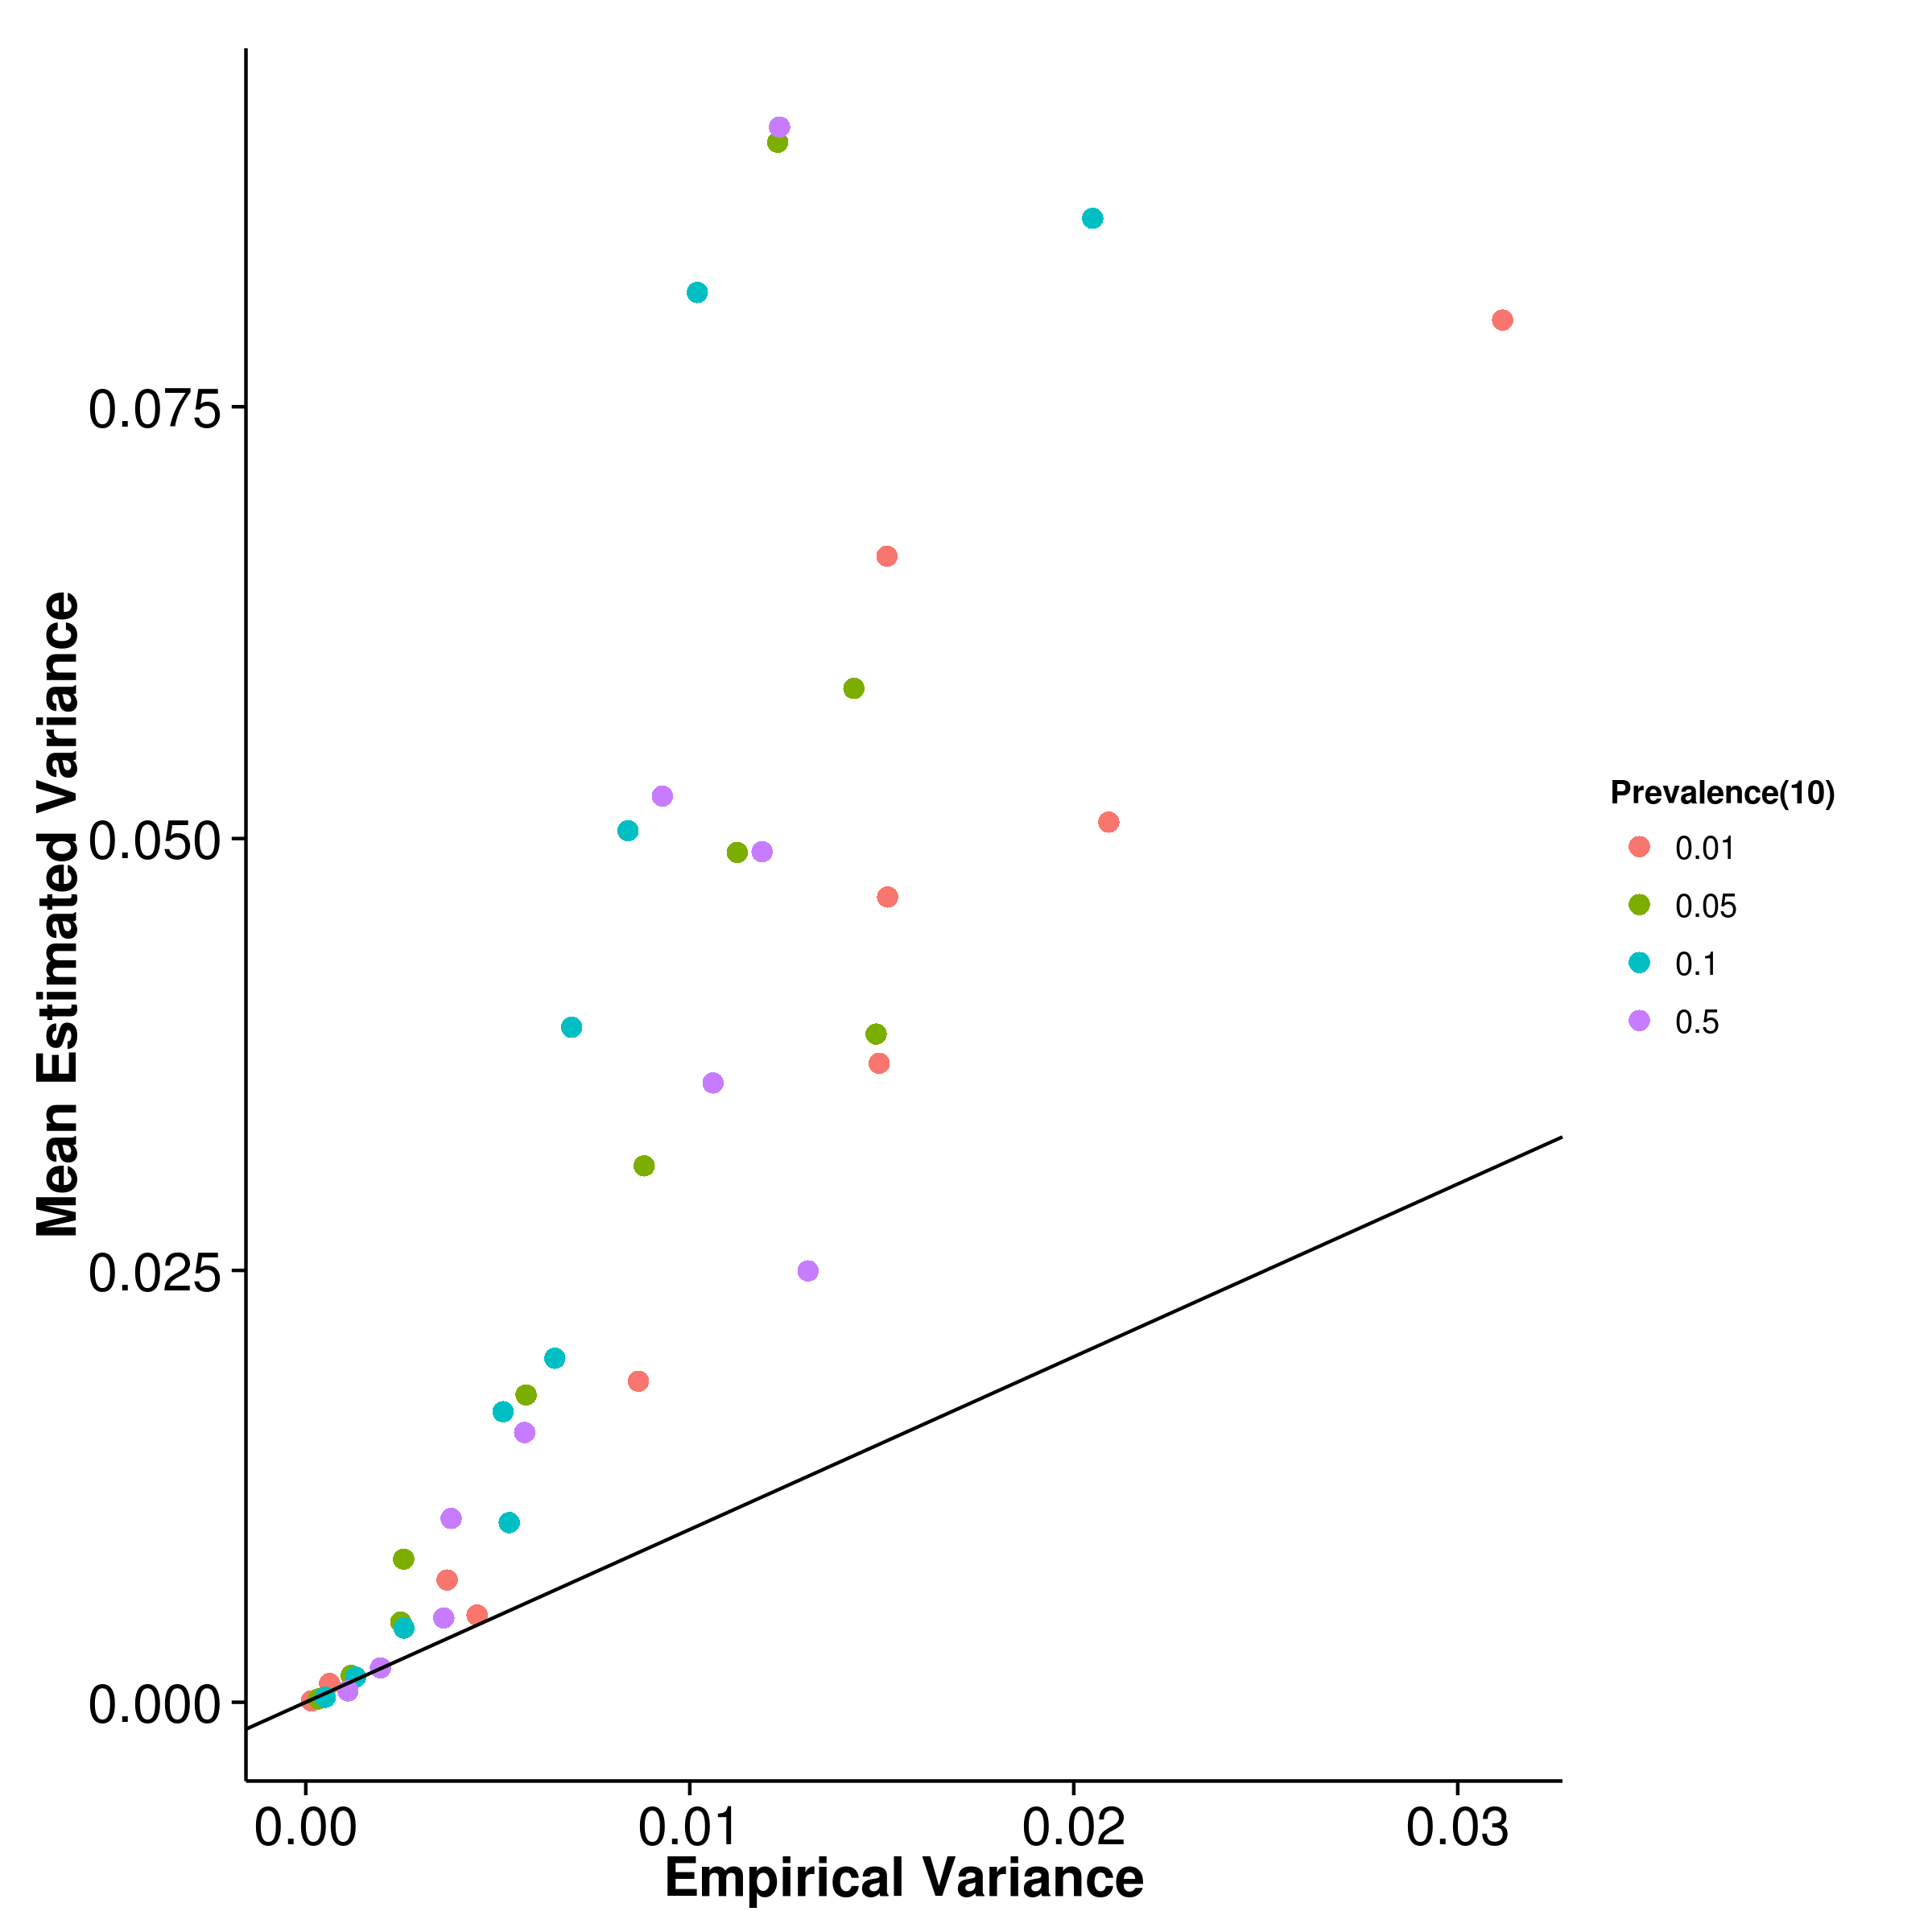
\includegraphics{figure/he_summary/cc_10c/ldsc_CC_Rand_sdCom.png}}
		\label{fig:ldscCC10RandVarCom}
	}
	\subfloat[LDSC with intercept estimation]{
		
		\scalebox{.4}{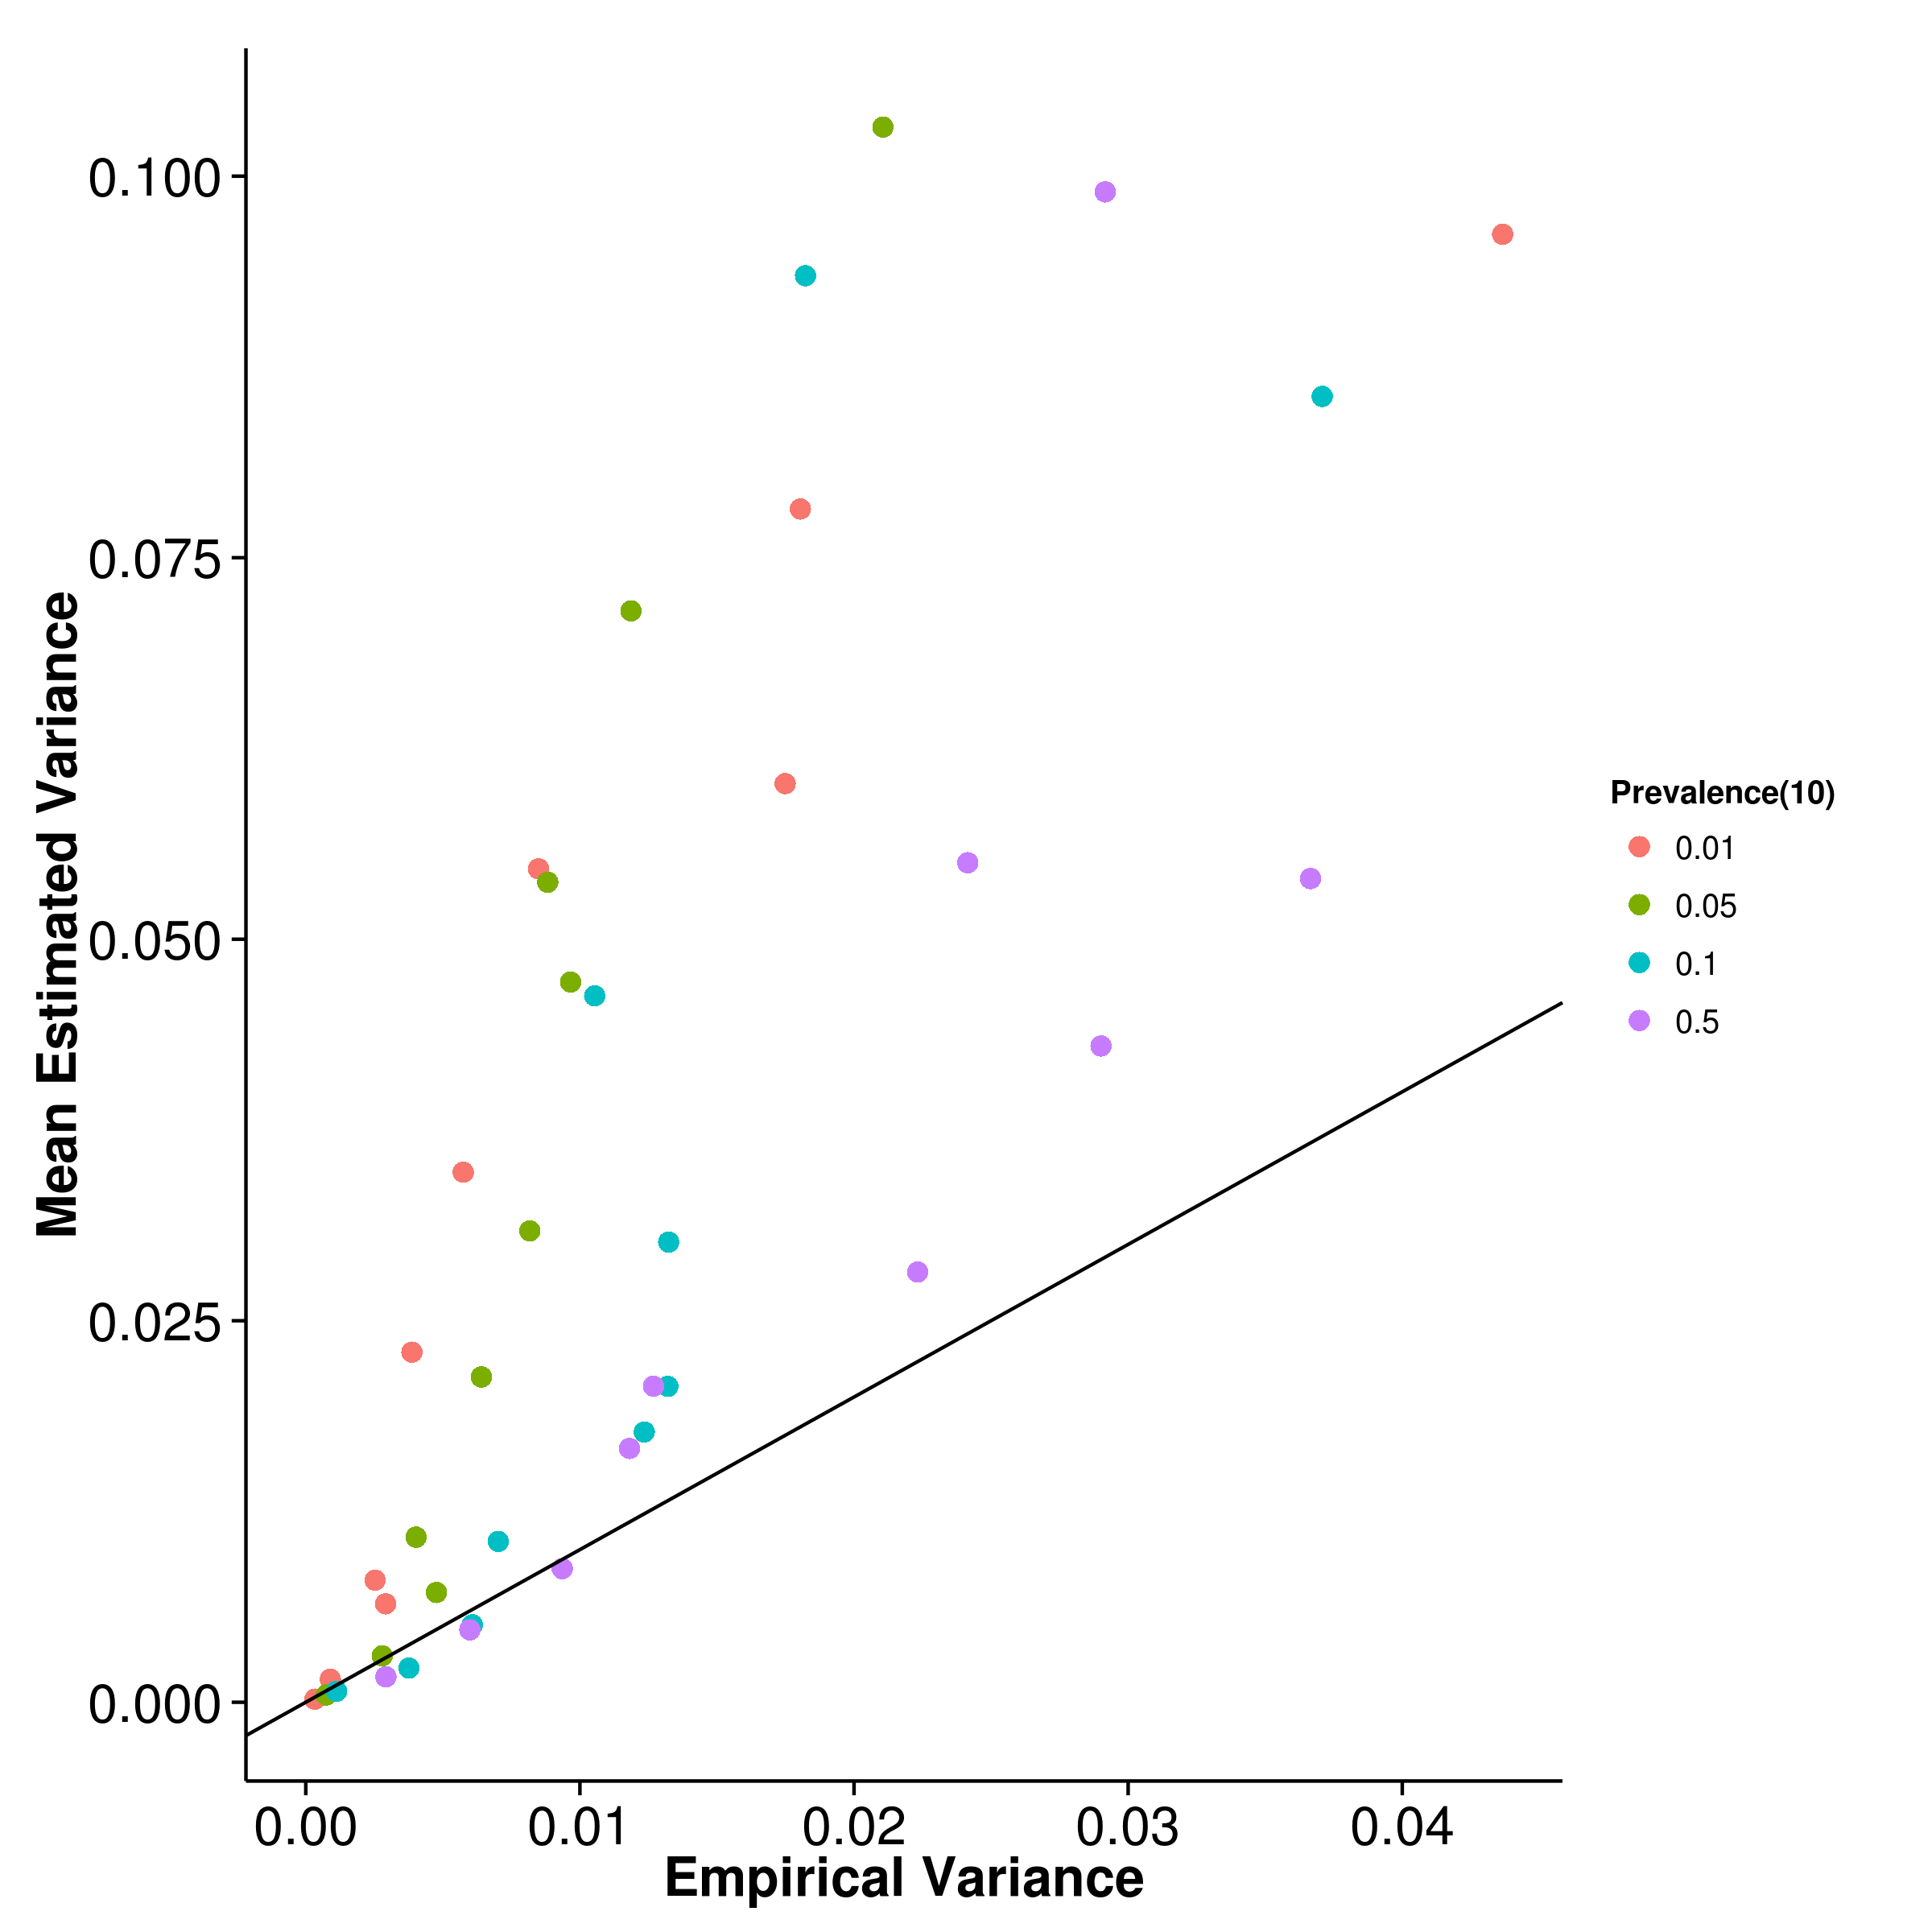
\includegraphics{figure/he_summary/cc_10c/ldscIn_CC_Rand_sdCom.png}}
		\label{fig:ldscInCC10RandVarCom}
	}
	\caption[Estimation of Variance in Binary Trait Simulation (10 Causal)]
	{Estimated variance of results from binary trait simulation with random effect size simulation when compared to empirical variance when 10 causal \glspl{SNP} was simulated.
		A general underestimation was observed for \gls{shrek} and \gls{gcta} whereas a larger upward bias was observed for \gls{ldsc}.} 
	\label{fig:CC10RandVarCom}
\end{figure}

To estimate the \gls{SNP}-heritability for binary traits, it is important to model the diseases status under a liability threshold model, which require knowledge of the population prevalence of the disease.
Due to the important influence of the population prevalence to the heritability, traits with different population prevalence were simulated such that the performance of \gls{ldsc} and \gls{shrek} can be assessed.

When only 10 causal \glspl{SNP} were simulated, it is clear that the population prevalence has a significant impact to the performance of the algorithms (\cref{fig:CC10RandMean}). 
Of all the algorithms tested, \gls{gcta} is the most affected by the population prevalence (\cref{fig:gctaCC10RandMean}), where the estimates are generally underestimated.
As the population prevalence decreases, the magnitude of bias increases, as reported by \citet{Golan2014}.
On the other hand, the estimates generated by \gls{ldsc} with fixed intercept and \gls{shrek} are upwardly biased with the magnitude of bias increases as the population prevalence decreases.
Surprisingly, when intercept estimation was performed, a downward bias is observed in the estimates from \gls{ldsc}.
The magnitude of bias is also relatively smaller when compared to \gls{ldsc} with fixed intercept.
The same pattern are observed when different number of causal \glspl{SNP} were simulated (\cref{fig:CC50RandMean,fig:CCRandMean,fig:CC500RandMean}).

Of all the algorithms, \gls{gcta} has the smallest average empirical variance (\cref{fig:gctaCC10RandVar}) and \gls{ldsc} with intercept estimation has the largest empirical variance.
On the other hand, it is observed that the estimates from \gls{shrek} (\cref{fig:shrekCC10RandVar}) and \gls{ldsc} (\cref{fig:ldscCC10RandVar}) with fixed intercept have similar empirical variance.
As the number of causal \glspl{SNP} increases, the empirical variance of all algorithms decreases (\cref{fig:CC50RandVar,fig:CCRandVar,fig:CC500RandVar}) similar to the results from the quantitative trait simulation.

It is observed that \gls{shrek} consistently underestimate its empirical variance where the magnitude of bias increases as population prevalence decreases (\cref{fig:shrekCC10RandVarCom}).
On the other hand, \gls{gcta} can provide a more accurate estimation for its empirical variance, only moderately underestimated the variance  (\cref{fig:gctaCC10RandVarCom}).
Again, it is observed that \gls{ldsc} consistently overestimate its empirical variance (\cref{fig:CC10RandVarCom}). 
However, as the number of causal \glspl{SNP} increases, the magnitude of bias observed in the estimation of variance decreases for \gls{ldsc} (\cref{fig:CC50RandVarCom,fig:CCRandVarCom,fig:CC500RandVarCom}). 
When 500 causal \glspl{SNP} were simulated, \gls{ldsc} can provide a relatively accurate estimates of its empirical variance (\cref{fig:ldscCC500RandVarCom}).

Overall, \gls{shrek} has the best average performance of all the algorithm tested (\cref{tab:mseCC}).
Interestingly, although no confounding factors were simulated, it is observed that \gls{ldsc} with intercept estimation has a better performance than \gls{ldsc} with fixed intercept when the prevalence is small.
Therefore, it is possible for the intercept estimation to help correcting for some of bias introduced by case control sampling.

\begin{table}
	\centering
	\begin{tabular}{p{2cm}p{2.4cm}rrrr}
		\toprule
		Population Prevalence&	Number of Causal SNPs&	SHREK&	LDSC&	LDSC-In&	GCTA \\
		\midrule
		0.01&	10&	\textbf{0.0145}&	0.0361&	0.0164&	0.0675\\
		0.01&	50&	0.0135&	0.0254&	\textbf{0.00791}&	0.0702\\
		0.01&	100&	0.0128&	0.0227&	\textbf{0.0102}&	0.0698\\
		0.01&	500&	\textbf{0.0126}&	0.0214&	0.0150&	0.0710\\
		0.05&	10&	0.0110&	0.0201&	\textbf{0.00983}&	0.0302\\
		0.05&	50&	\textbf{0.00453}&	0.00974&	0.0115&	0.0299\\
		0.05&	100&	\textbf{0.00569}&	0.0113&	0.00981&	0.0304\\
		0.05&	500&	\textbf{0.00540}&	0.00999&	0.0171&	0.0305\\
		0.1&	10&	\textbf{0.00512}&	0.0109&	0.0301&	0.0165\\
		0.1&	50&	\textbf{0.00381}&	0.00824&	0.0105&	0.0152\\
		0.1&	100&	\textbf{0.00418}&	0.00802&	0.0163&	0.0148\\
		0.1&	500&	\textbf{0.00400}&	0.00740&	0.0141&	0.0155\\
		0.5&	10&	0.00560&	0.00749&	0.0219&	\textbf{0.00410}\\
		0.5&	50&	0.00362&	0.00528&	0.0232&	\textbf{0.00244}\\
		0.5&	100&	0.00356&	0.00460&	0.0208&	\textbf{0.00225}\\
		0.5&	500&	0.00338&	0.00365&	0.0159&	\textbf{0.00200}\\
		\bottomrule
	\end{tabular}
	\caption[MSE of Binary Trait Simulation]{
		\Gls{mse} of Binary Trait simulation.
		Algorithm with the best performance under each condition were \textbf{bold-ed}.
		Of all the algorithms, \gls{shrek} has the best average performance.
		It is observed that as the number of causal \glspl{SNP} increases, the \gls{mse} tends to decrease for all algorithms, similar to the results from quantitative trait simulation.
	}
	\label{tab:mseCC}
\end{table}

It is noted that when compared to the quantitative trait simulation, a smaller number of \glspl{SNP} and larger sample size (2,000 samples with 1,000 cases and 1,000 controls) were simulated. 
Thus, the results from binary trait simulations are not directly comparable to the results from the quantitative trait simulations.

\subsubsection{Extreme Phenotype Simulation}
%Mean
\begin{figure}
	\centering
	\subfloat[SHREK]{
		\scalebox{.4}{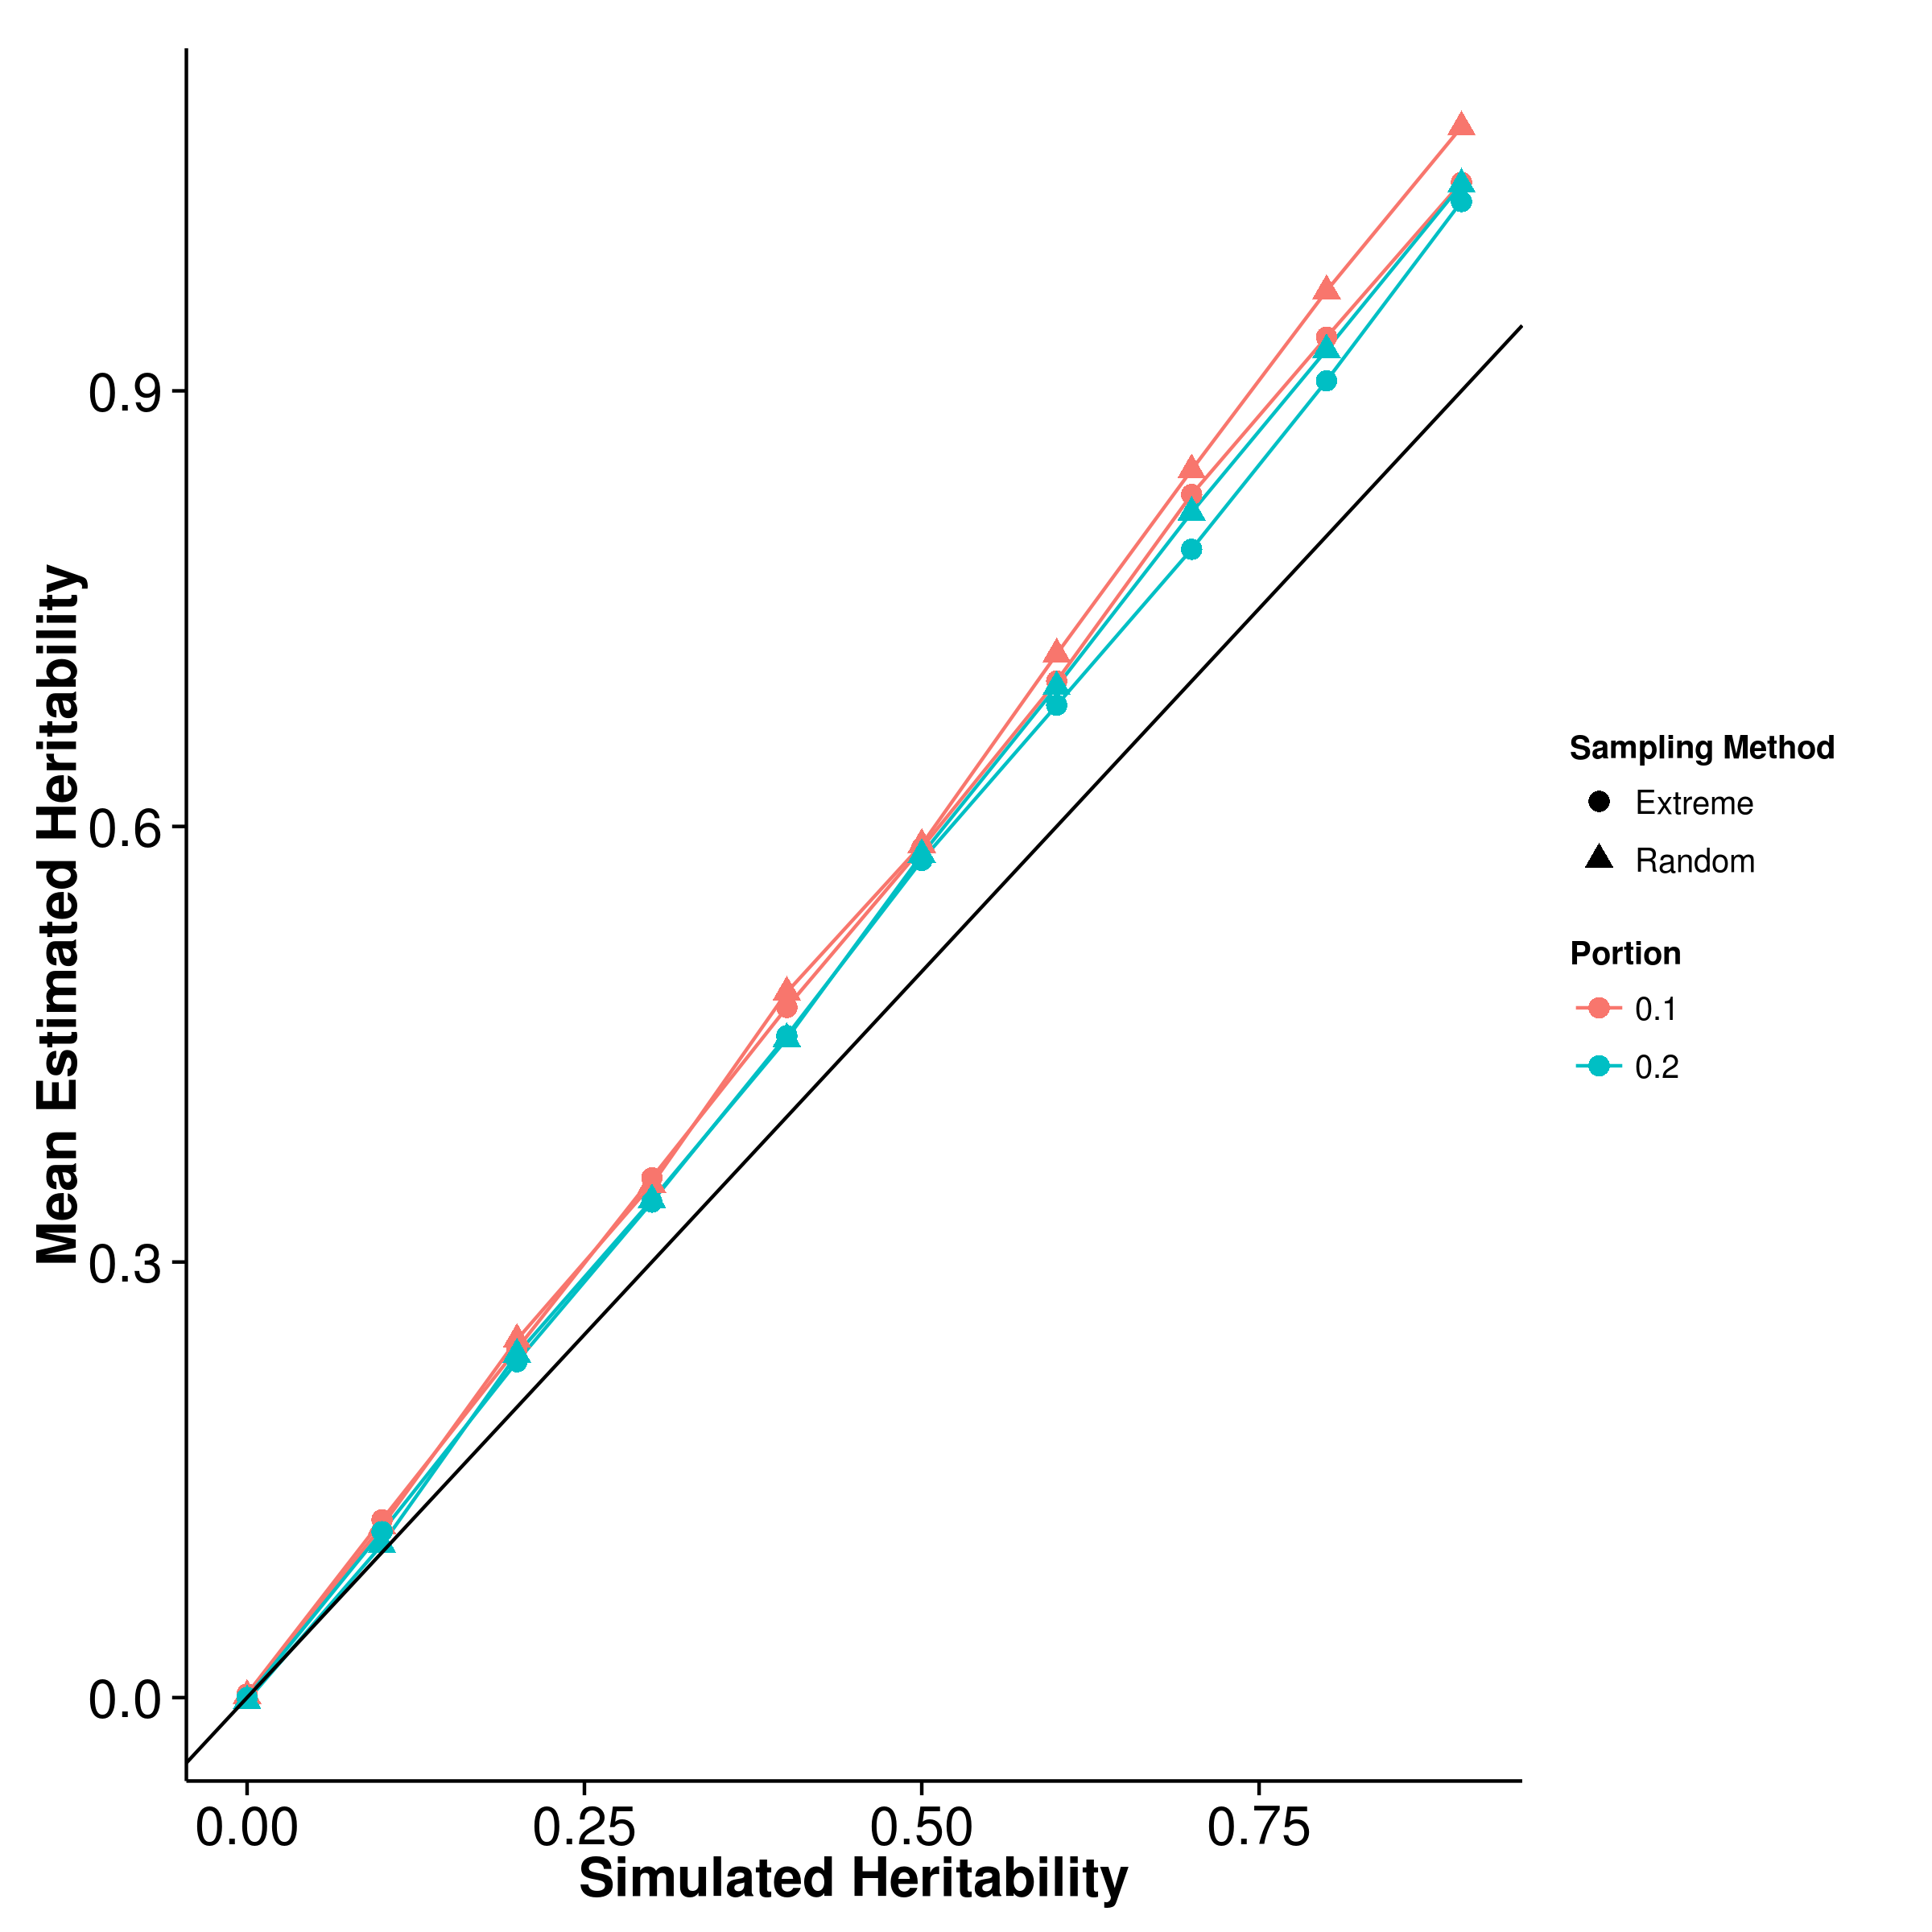
\includegraphics{figure/he_summary/pheno_extreme/shrek_extremeSelect_mean.png}}
		\label{fig:shrekExMean}
	}
	\subfloat[GCTA]{
		\scalebox{.4}{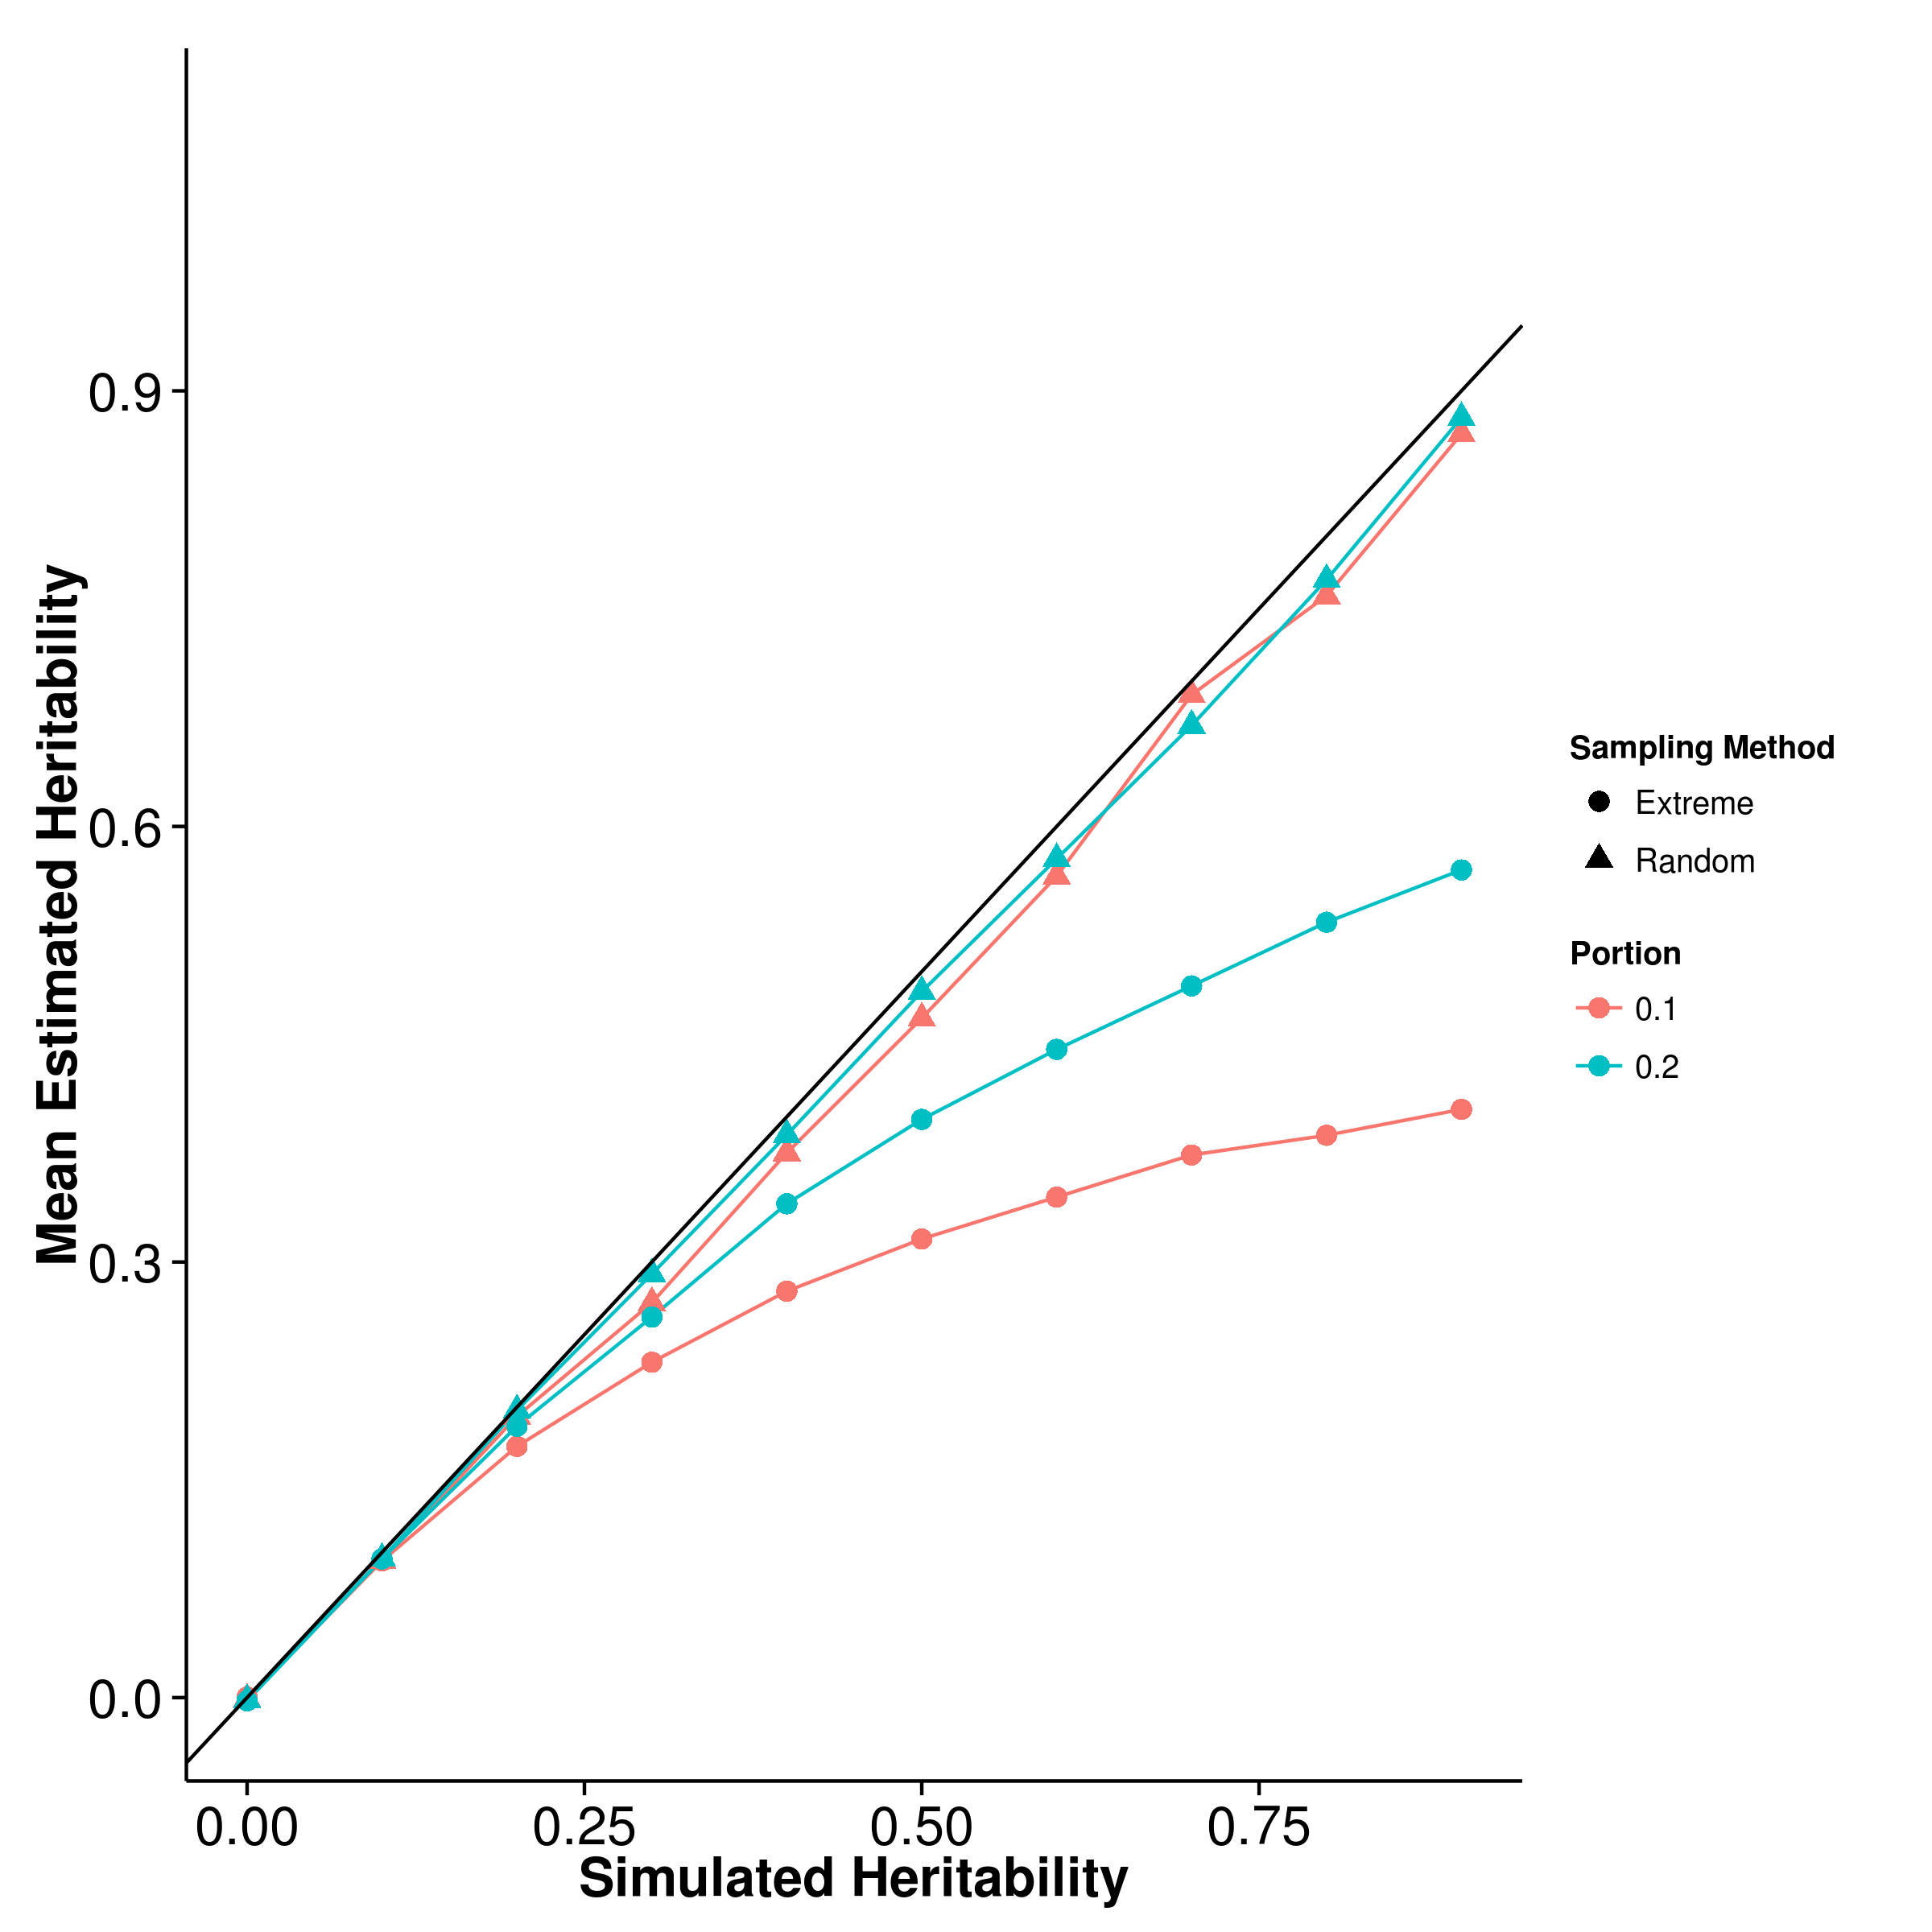
\includegraphics{figure/he_summary/pheno_extreme/gcta_extremeSelect_mean.png}}
		\label{fig:gctaExMean}
	}\\
	\subfloat[LDSC with fix intercept]{
		\scalebox{.4}{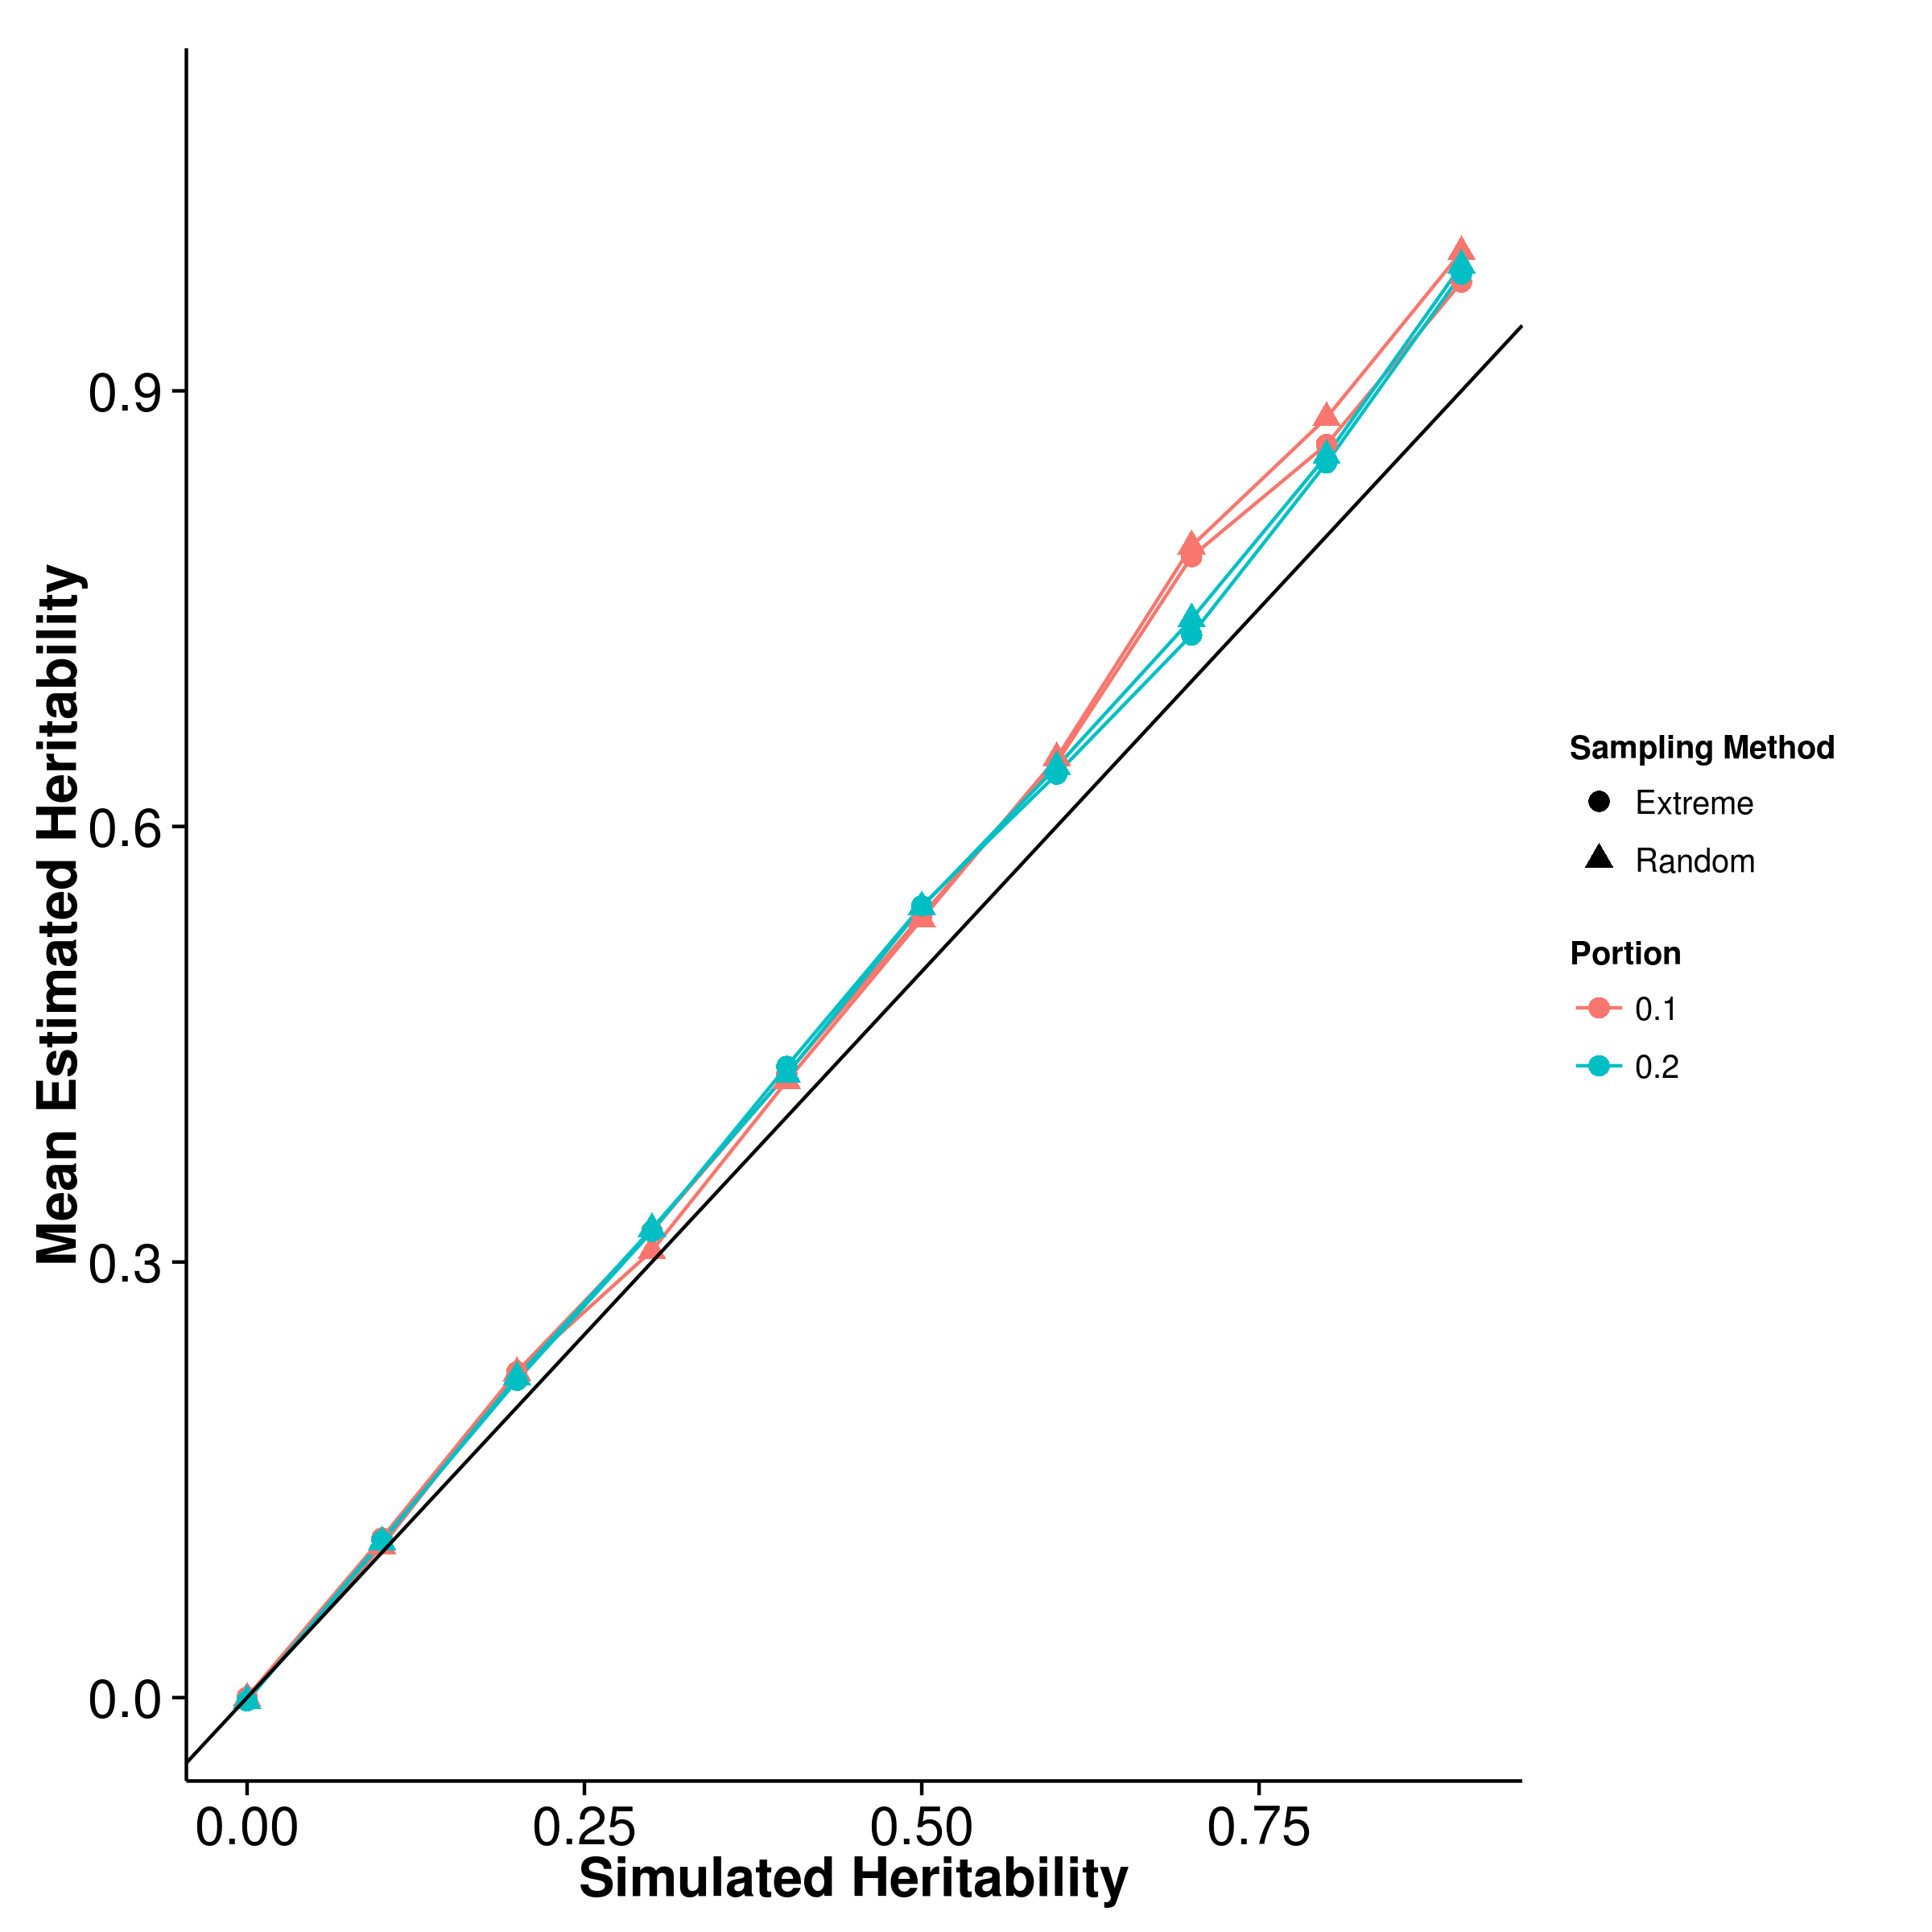
\includegraphics{figure/he_summary/pheno_extreme/ldsc_extremeSelect_mean.png}}
		\label{fig:ldscExMean}
	}
	\subfloat[LDSC with intercept estimation]{
		
		\scalebox{.4}{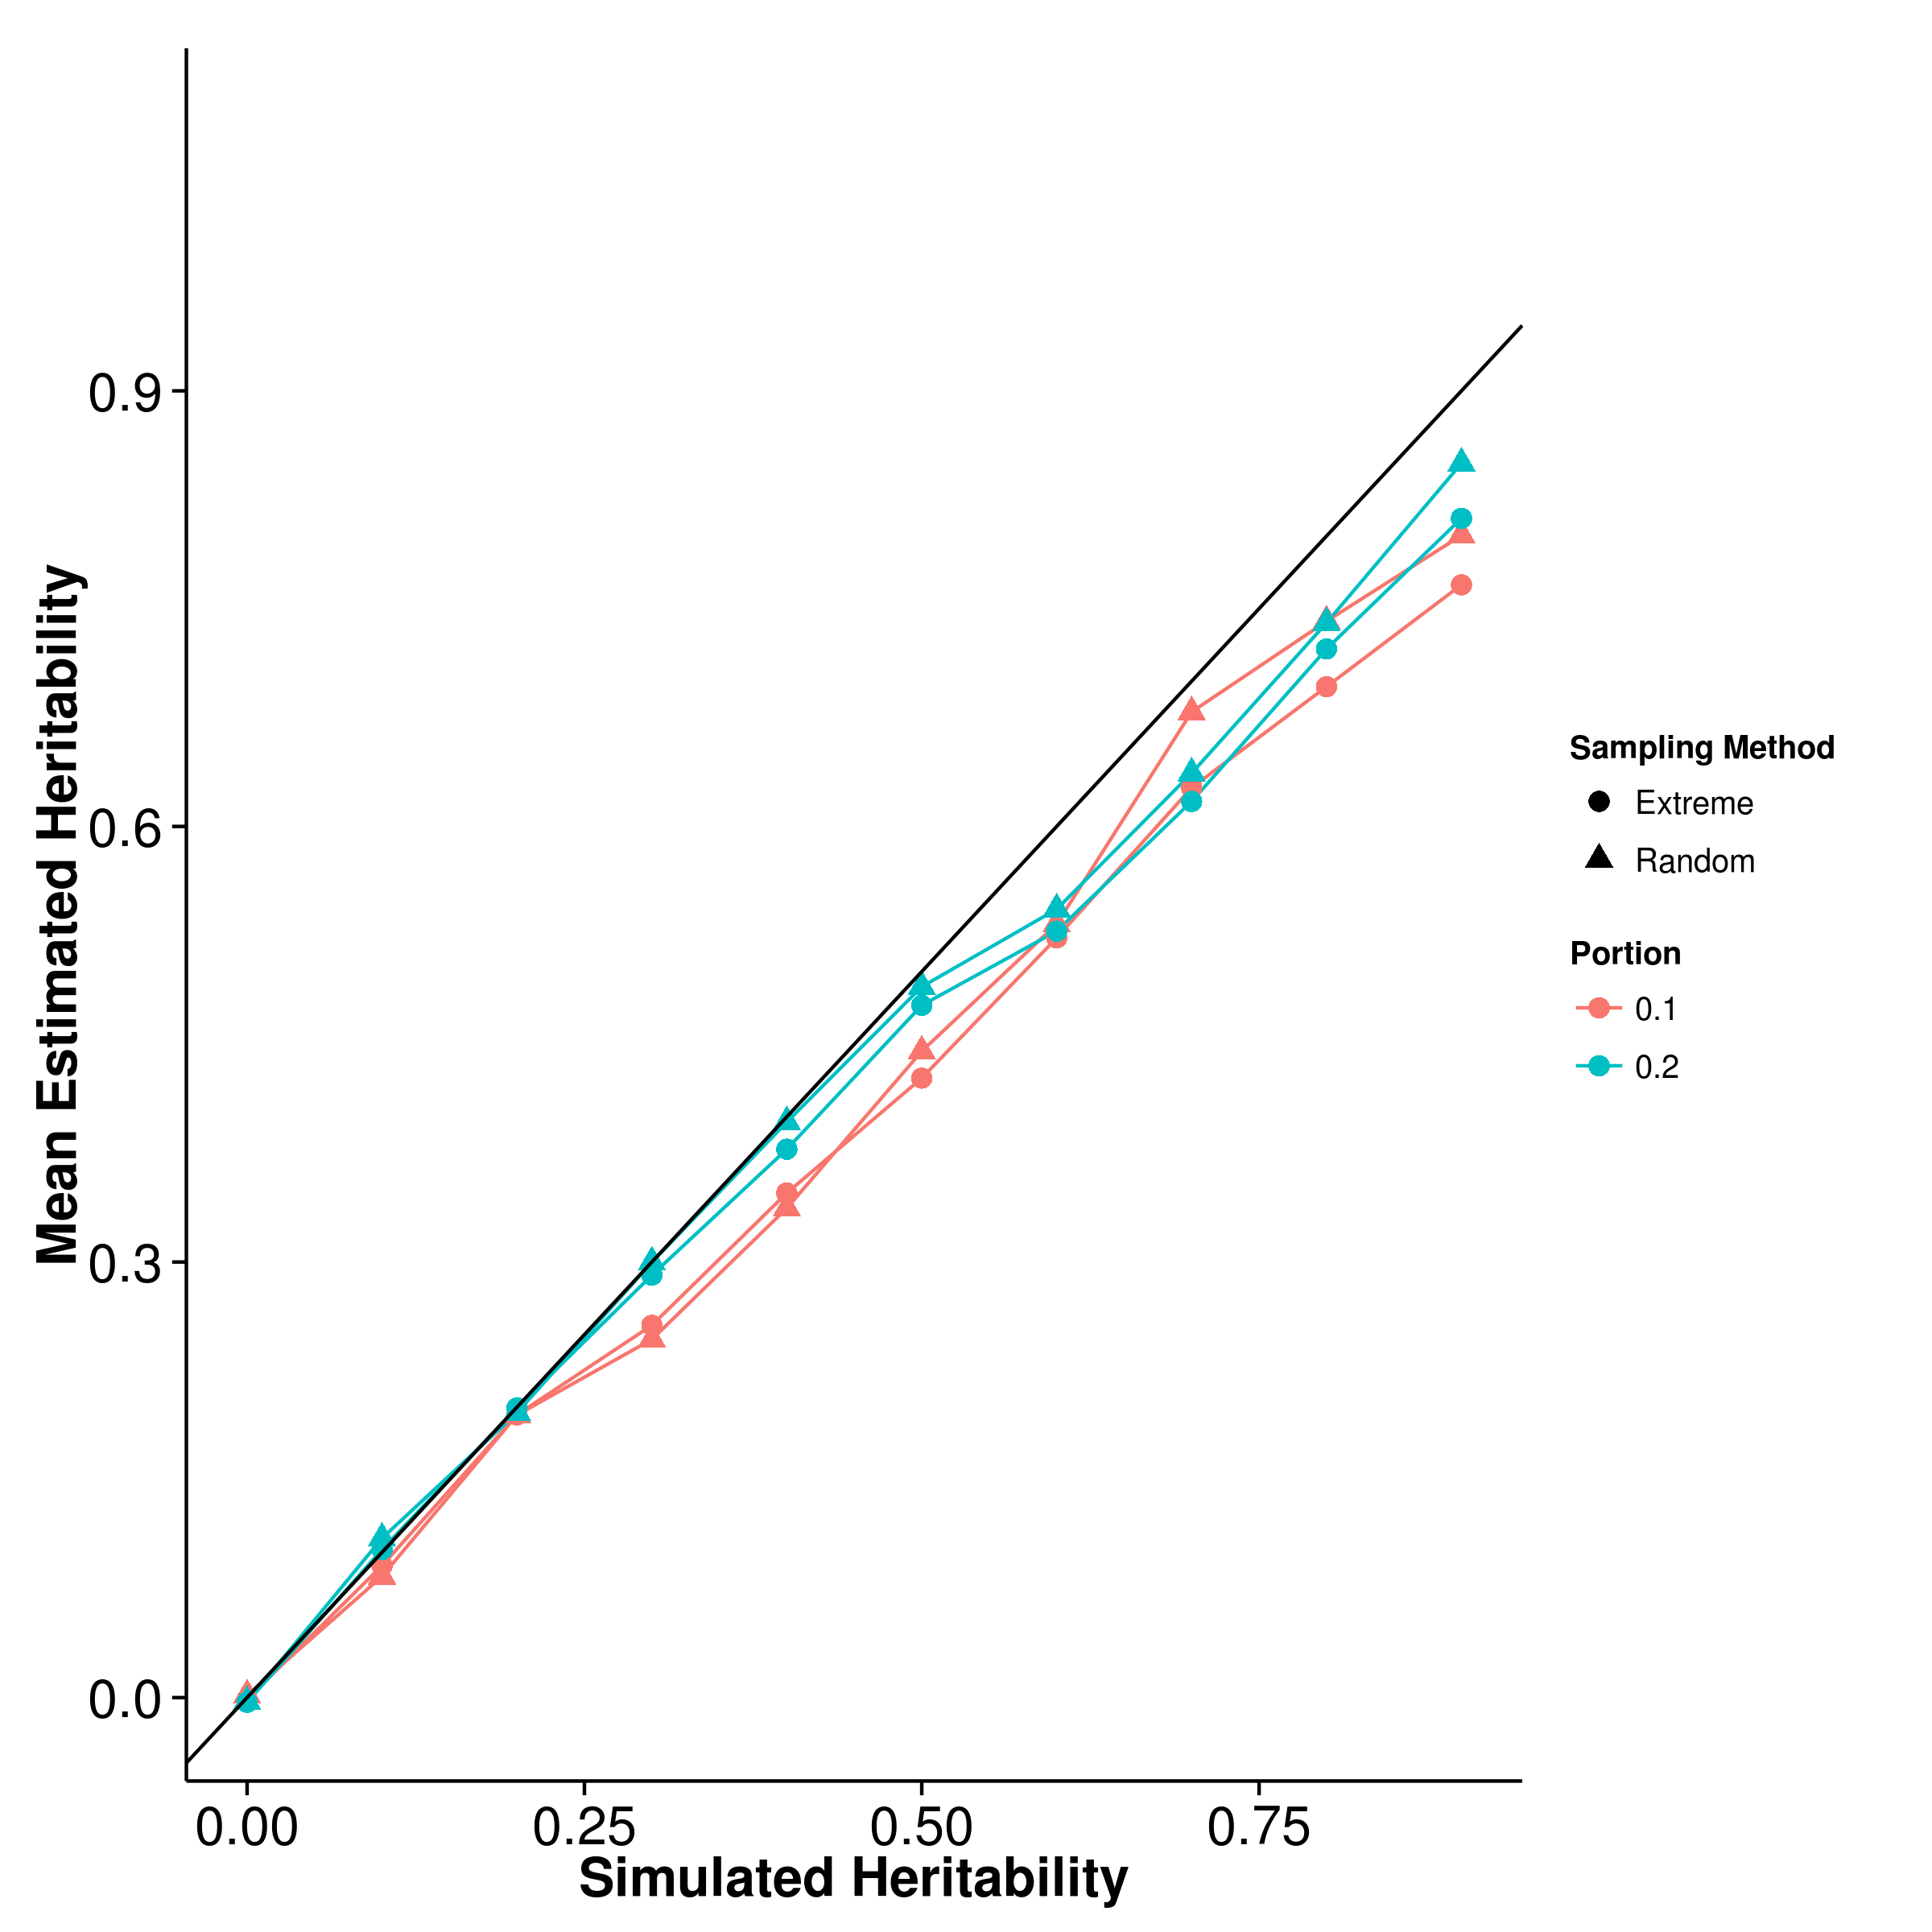
\includegraphics{figure/he_summary/pheno_extreme/ldscIn_extremeSelect_mean.png}}
		\label{fig:ldscInExMean}
	}
	\caption[Mean of Extreme Phenotype Selection Simulation Results]
	{Mean of results from extreme phenotype simulation.
		The performance of the algorithms when random sampling was performed were similar to what was observed in the quantitative trait simulation.
		However, when extreme phenotype was performed, a larger under estimation was observed for \gls{gcta} and it gets worst when the portion of sample selected decreases.
		On the other hand, the performance of \gls{shrek} and \gls{ldsc} under the extreme phenotype selection was similar to that from the random samplings.
	} 
	\label{fig:ExMean}
\end{figure}
%Empirical Variance
\begin{figure}
	\centering
	\subfloat[SHREK]{
		\scalebox{.4}{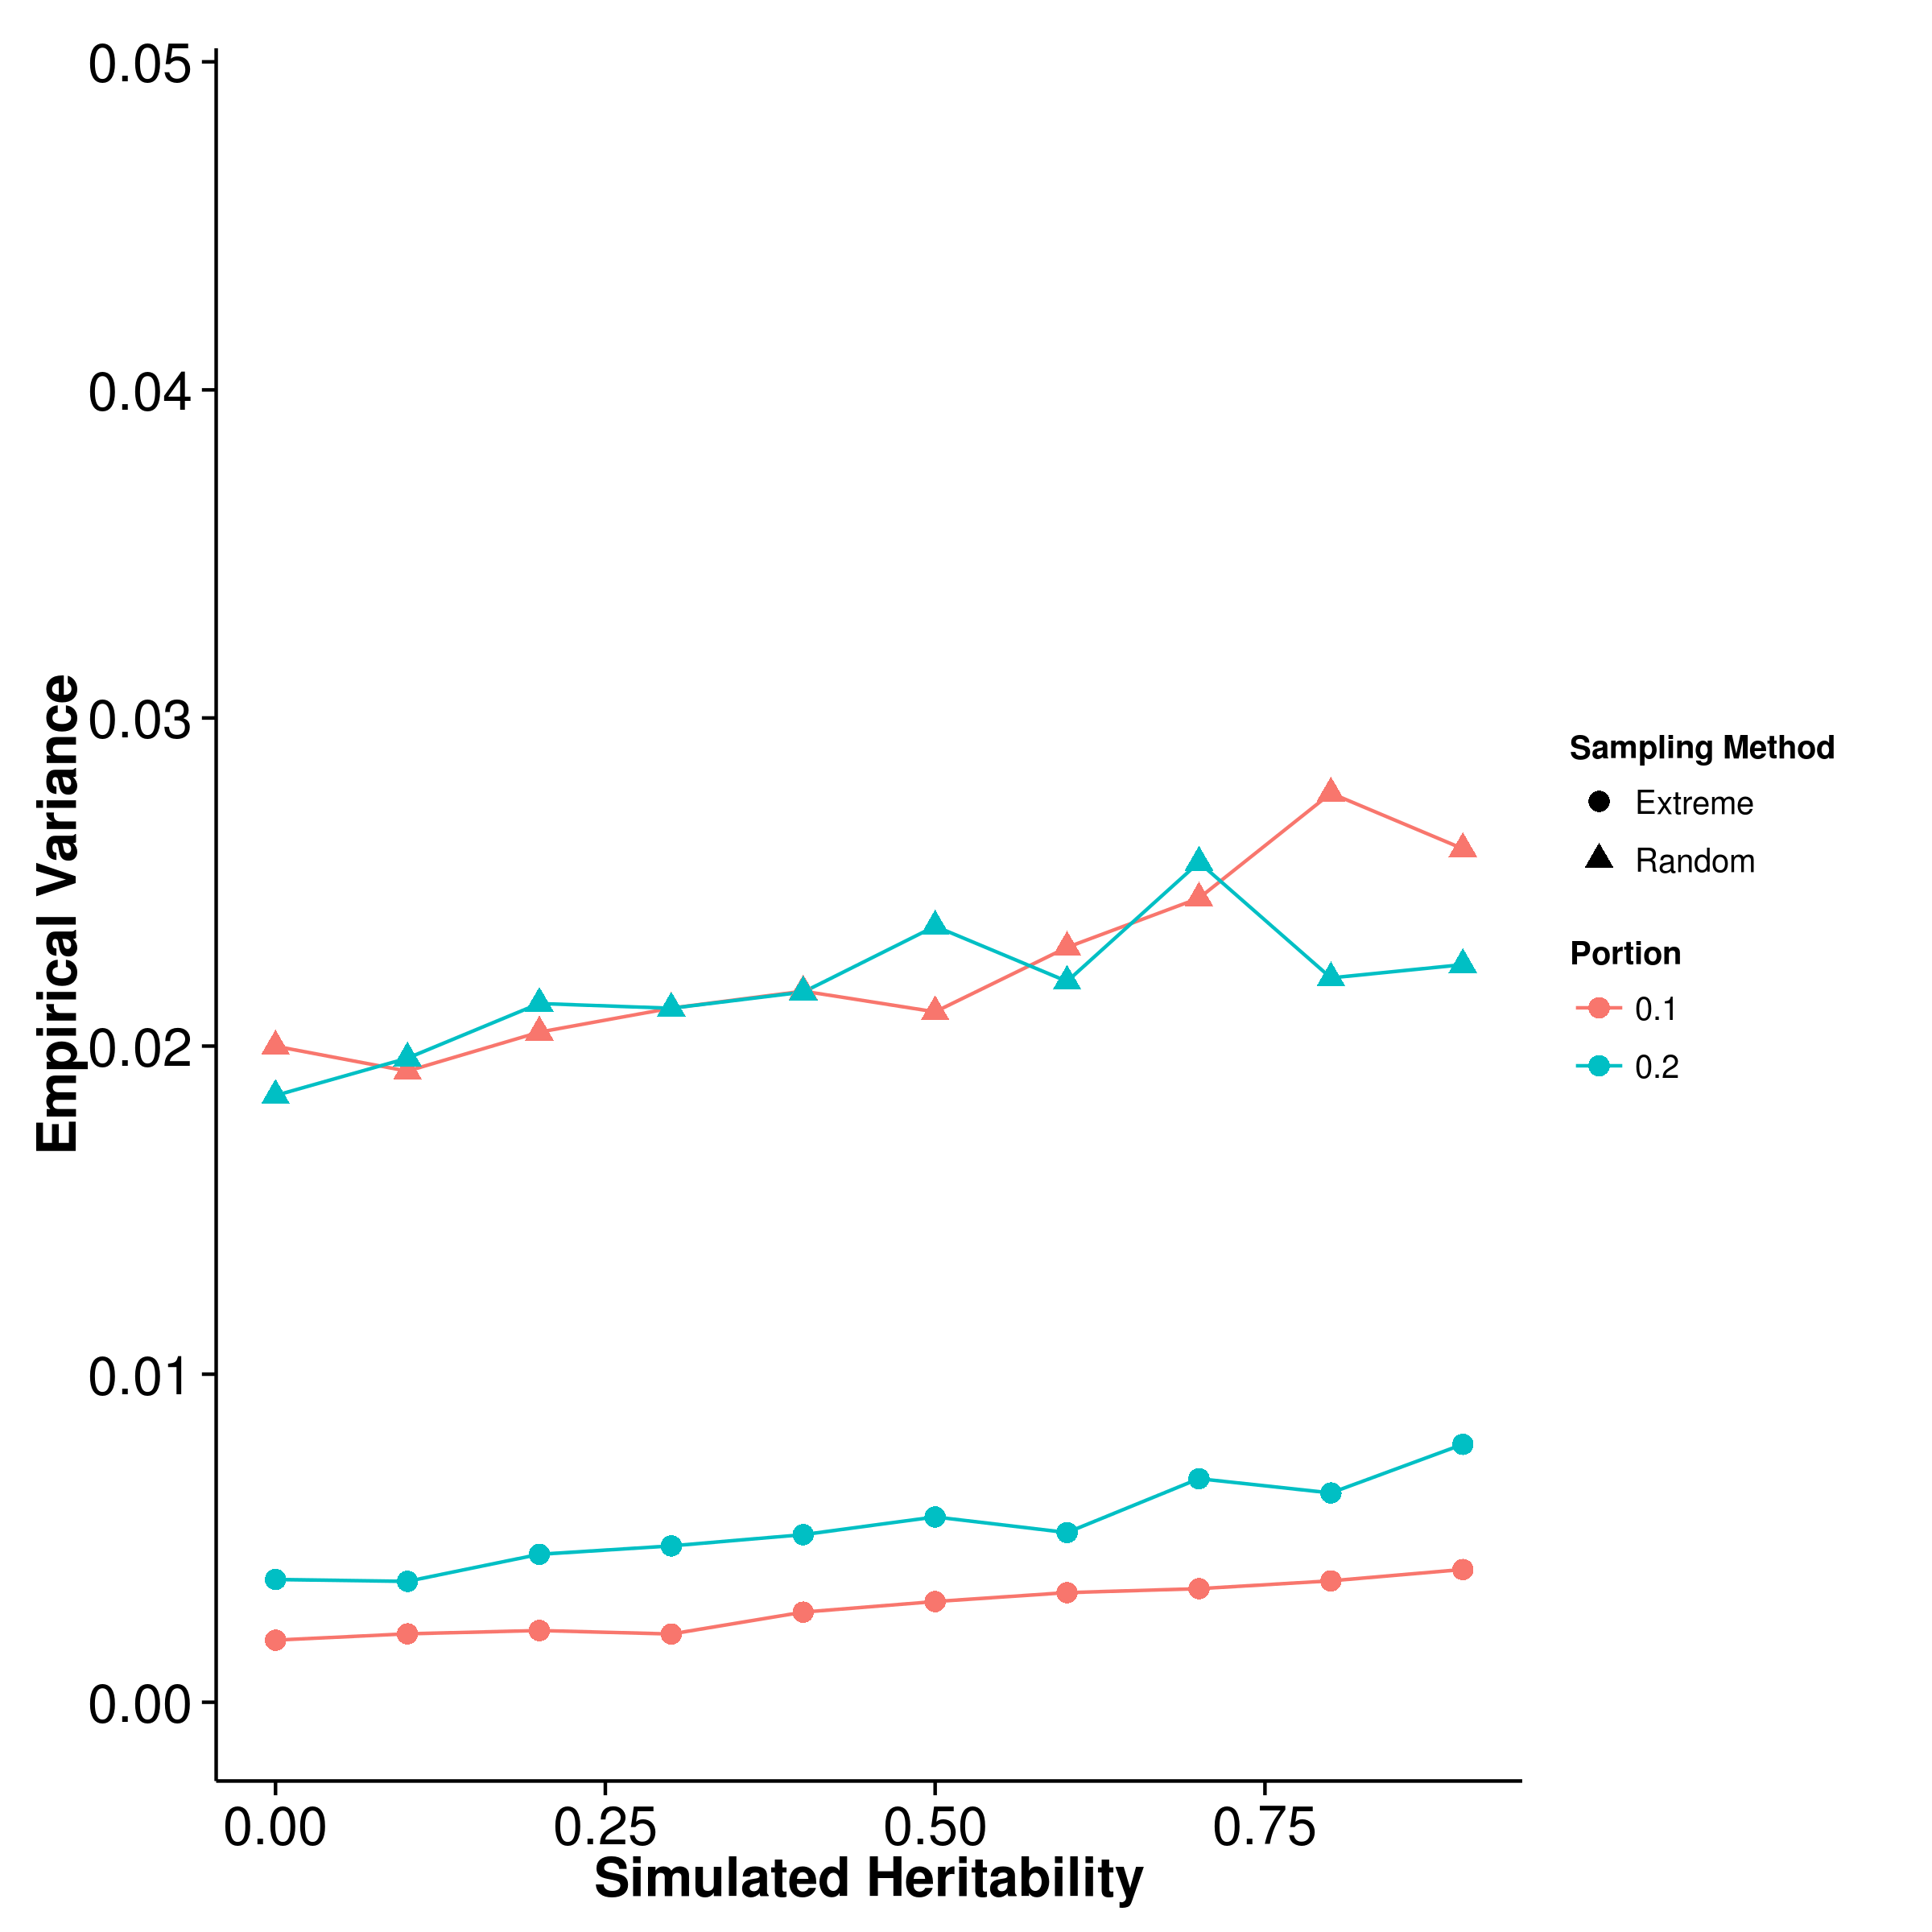
\includegraphics{figure/he_summary/pheno_extreme/shrek_extremeSelect_var.png}}
		\label{fig:shrekExVar}
	}
	\subfloat[GCTA]{
		\scalebox{.4}{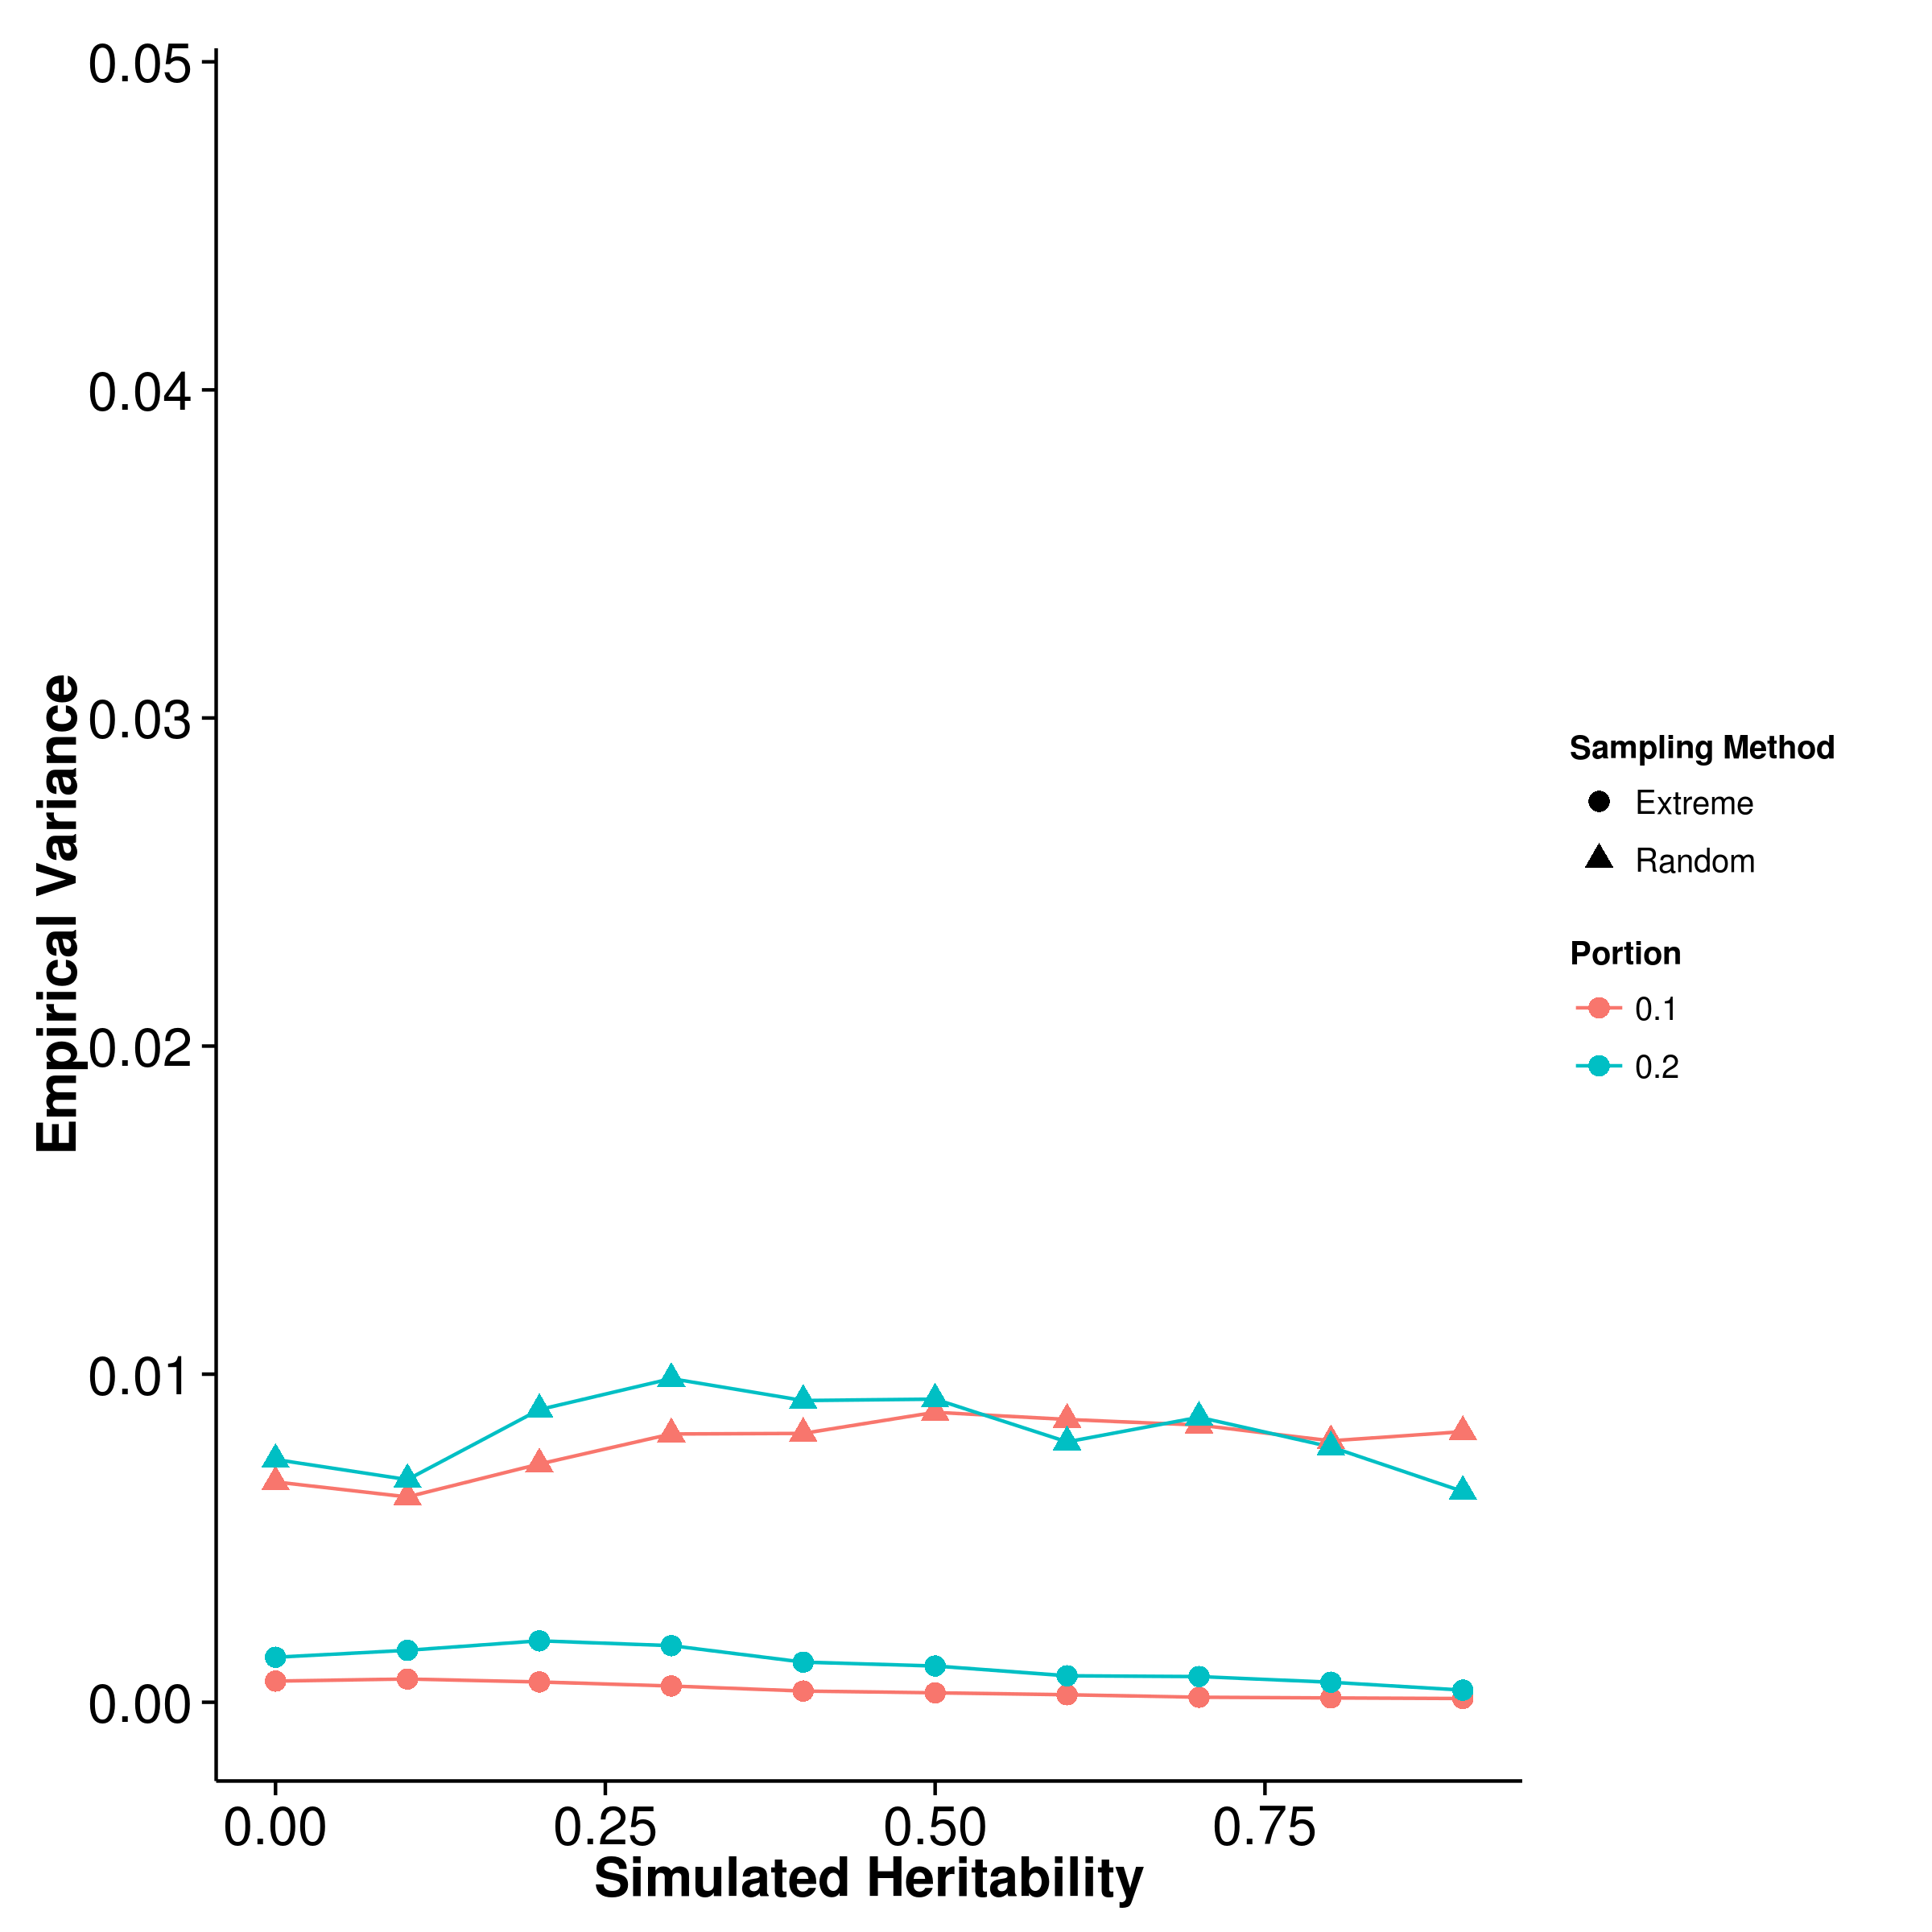
\includegraphics{figure/he_summary/pheno_extreme/gcta_extremeSelect_var.png}}
		\label{fig:gctaExVar}
	}\\
	\subfloat[LDSC with fix intercept]{
		\scalebox{.4}{\includegraphics{figure/he_summary/pheno_extreme/ldsc_extremeSelect_var.png}}
		\label{fig:ldscEx}
	}
	\subfloat[LDSC with intercept estimation]{
		
		\scalebox{.4}{\includegraphics{figure/he_summary/pheno_extreme/ldscIn_extremeSelect_var.png}}
		\label{fig:ldscInExVar}
	}
	\caption[Variance of Extreme Phenotype Selection Simulation Results]
	{Variance of results from extreme phenotype simulation.
		It is obvious that when the extreme phenotype selection was performed, the empirical variance of all the algorithm decreases and is much smaller than the empirical variance of the estimation when random sampling was performed.
		We also compared the empirical variance of random sampling with those from quantitative trait simulation with 100 causal \glspl{SNP} and they are highly similar. 
	} 
	\label{fig:ExVar}
\end{figure}
%Variance Estimation
\begin{figure}
	\centering
	\subfloat[SHREK]{
		\scalebox{.4}{\includegraphics{figure/he_summary/pheno_extreme/shrek_extremeSelect_varCom.png}}
		\label{fig:shrekExVarCom}
	}
	\subfloat[GCTA]{
		\scalebox{.4}{\includegraphics{figure/he_summary/pheno_extreme/gcta_extremeSelect_varCom.png}}
		\label{fig:gctaExVarCom}
	}\\
	\subfloat[LDSC with fix intercept]{
		\scalebox{.4}{\includegraphics{figure/he_summary/pheno_extreme/ldsc_extremeSelect_varCom.png}}
		\label{fig:ldscExVarCom}
	}
	\subfloat[LDSC with intercept estimation]{
		
		\scalebox{.4}{\includegraphics{figure/he_summary/pheno_extreme/ldscIn_extremeSelect_varCom.png}}
		\label{fig:ldscInExVarCom}
	}
	\caption[Estimation of Variance in Extreme Phenotype Selection]
	{Estimated variance of results from extreme phenotype selection when compared to empirical variance.
		Surprisingly, except for \gls{shrek}, the estimated variance from \gls{ldsc} and \gls{gcta} under the random sampling condition was much higher than the empirical variance. 
		It is much different from the estimated variance from the quantitative trait simulation and further investigations are required to understand this discrepancy.
	} 
	\label{fig:ExVarCom}
\end{figure}

By using appropriate sampling strategy, such as extreme phenotype sampling \citep{Peloso2015}, one can increase the power of the association study.
However, it is unclear how the extreme phenotype sampling will affect the performance of the \gls{SNP} heritability estimation.
Therefore, simulations were performed to investigate the effect of extreme phenotype sampling on \gls{SNP} heritability estimation compared to random sampling approach. 

It is observed that when the extreme phenotype sampling was performed, the estimates from \gls{gcta} biased downward in pattern similar to what was observed in the binary trait simulation (\cref{fig:gctaExMean}).
On the other hand, estimates from \gls{shrek} and \gls{ldsc} with fixed intercepts are slightly inflated whereas \gls{ldsc} with intercept estimation slightly underestimated the \gls{SNP} heritability (\cref{fig:ExMean}).

When comparing the empirical variance, the random sampling consistently results in a larger empirical variance in the estimates of the algorithms (\cref{tab:ratioEx}).	
It is observed that when random sampling were performed, the resulting empirical variance from the algorithms are similar to the results in the quantitative trait simulation. 
However, there is a large discrepancy in the estimated variance of \gls{ldsc} and \gls{gcta}, where there can be as much as a tenfold difference (\cref{fig:ExVarCom}). 
On the other hand, the estimated variance of \gls{shrek} is unaffected.
It is unclear what induces the inflation and further investigations are therefore required.

\begin{table}[H]
	\centering
	\begin{tabular}{rrrrrrrrr}
		\toprule
		\multirow{2}[4]{*}{Portion} & \multicolumn{2}{c}{Shrek} & \multicolumn{2}{c}{LDSC} & \multicolumn{2}{c}{LDSC-In} & \multicolumn{2}{c}{GCTA} \\
		& Extreme & Rand & Extreme & Rand & Extreme & Rand & Extreme & Rand\\
		\midrule
		0.1   & 0.0113 & 0.0341 & 0.00537 & 0.0167 & 0.0119 & 0.0329 & 0.0644 & 0.00849 \\
		0.2   & 0.0109 & 0.0290 & 0.00599 & 0.0152 & 0.0126 & 0.0299 & 0.0274 & 0.00852 \\
		\bottomrule
	\end{tabular}
	\caption[Comparing the MSE of Extreme Phenotype Sampling and Random Sampling]{
		Comparing the \gls{mse} of extreme phenotype sampling (Extreme) and random sampling (Rand).
		With the exception of \gls{gcta}, the extreme phenotype sampling will results in a smaller \gls{mse} given the same amount of samples.
	}
	\label{tab:ratioEx}
\end{table}

\subsection{Application to Real Data}
The main purpose of the current chapter is to test whether if the \gls{SNP}-heritability of \scz\ estimated by \citet{Bulik-Sullivan2015} is correct. 
Therefore, we estimated the heritability of \scz, together with major depression disorder and bipolar with \gls{shrek} and \gls{ldsc}.
Surprisingly, the estimated \gls{SNP}-heritability for all disorder investigated are very different from the estimated provided in the \citet{Bulik-Sullivan2015} paper (\cref{tab:realData}).
Contrary to the previous estimate, the common \glspl{SNP} accounts for no more than 20\% of the heritability of \scz, which suggest that other genetic factors such as rare variants and epigenetic changes might also contribute to the heritability of \scz.
\begin{table}[H]
	\centering
	\begin{tabular}{rrrr}
		\toprule
		\\
		& \begin{tabular}[x]{@{}c@{}}Major Depression\\ Disorder\end{tabular} & Bipolar & \Scz\\
		\midrule		
		\gls{shrek} & 0.252 (0.0273)& 0.308 (0.0167) & 0.185 (0.00450) \\ 
		\gls{ldsc} & 0.232 (0.0217) & 0.265 (0.0152) & 0.198 (0.0057) \\
		\gls{ldsc}-In & 0.154 (0.033) & 0.181 (0.0203) & 0.135 (0.0072) \\
		\citet{Bulik-Sullivan2015} & 0.409 (0.033) & 0.531 (0.022) & 0.555 (0.008)\\
		\bottomrule
	\end{tabular}
	\caption[Heritability Estimated for PGC Data Sets]{
		Heritability estimated for \gls{pgc} data sets.
		The heritability estimated from \gls{ldsc} when intercept estimation was performed (\gls{ldsc}-In) are lower than the estimates from \gls{shrek} and \gls{ldsc} with fixed intercept.
		As the intercept estimation was used for the correction of confounding effects such as population stratifications or cryptic relatedness, the larger estimates from \gls{shrek} and \gls{ldsc} might be a result of the confounding effects.
	}
	\label{tab:realData}
\end{table}

\section{Discussion}
\Scz\ is a devastating disorder which is of our greatest interest to understand its disease etiology. 
Recently, in the paper by \citet{Bulik-Sullivan2015}, the authors estimated that the \gls{SNP}-heritability of \scz\ accounts for majority of the heritability of the disease.
However, considering that other genetic variations such as rare mutations and \gls{cnv} are also associated with \scz, together with the possible presence of the gene-environment interaction, the \gls{SNP}-heritability of \scz\ estimated by \citet{Bulik-Sullivan2015} might be too high.
Therefore, we set off to develop an alternative algorithm, \gls{shrek} for the estimation of \gls{SNP}-heritability without requiring the individual genotypes, such that we can compare the estimates from the two programme and investigate whether if the estimates from \citet{Bulik-Sullivan2015} is correct.
Additionally, we also performed a comprehensive simulation to study the performance of both \gls{ldsc} and \gls{shrek} when handling traits with different genetic architectures. 

\subsection{LD Correction}
Similar to \gls{ldsc}, \gls{shrek} relies heavily on the \gls{LD} information for the estimation of the \gls{SNP}-heritability. 
Therefore, it is vital to obtain an accurate estimate of the \gls{LD} where any sampling errors should be adjusted. 

When comparing different bias correction algorithms from \cref{sec:ldSim}, it was observed that the equation from \citet{Weir1980} \cref{eq:weir} has the best performance. 
Therefore, it was selected as the default bias correction algorithm.

By applying the \gls{LD} correction algorithm, we hope to obtain a more accurate estimate.
However, in the subsequent simulations, an upward bias is consistently observed in the estimates from \gls{shrek}, which resemble to the inflation observed in the \gls{LD} correction simulation. 
Considering that a much smaller number of \glspl{SNP} were simulated in the \gls{LD} correction simulation, it is possible that the inflation was caused by an increased number of \glspl{SNP} in the genome.

It is also observed that although \gls{ldsc} also relies on the \gls{LD} information, the same overestimation is not observed.
Upon detail inspection of the algorithm of \gls{ldsc}, it was found that \gls{ldsc} employed a different \gls{LD} correction algorithm:
\begin{equation}
\text{LDSC}: \tilde{R^2}= \hat{R^2}-\frac{1-\hat{R^2}}{n-2}\label{eq:ldscR2} 
\end{equation}

To test our hypothesis and also inspect the performance of the \gls{LD} correction algorithm from \gls{ldsc} in \gls{shrek}, an additional simulation was performed where a larger number of \glspl{SNP} were simulated (e.g. 50,000 \glspl{SNP} on chromosome 1).

\begin{figure}[t]
	\centering
	\subfloat[Mean Estimation]{
		\scalebox{.4}{\includegraphics{figure/quantitative/ld_correct/ldCom_mean_b.png}}
		\label{fig:bigmeanLDCor}
	}
	\subfloat[Empirical Variance]{
		\scalebox{.4}{\includegraphics{figure/quantitative/ld_correct/ldCom_var_b.png}}
		\label{fig:bigvarLDCor}
	}
	\caption[Effect of LD correction to Heritability Estimation with 50,000 SNPs]
	{Effect of LD correction to Heritability Estimation when 50,000 \glspl{SNP} were simulated.
		It is observed that all \gls{LD} correction algorithms inflate the estimates when large number of \glspl{SNP} were simulated.
		Interestingly, least amount of bias is observed when no \gls{LD} correction was performed.
	} 
	\label{fig:ldCorBigCom}
\end{figure}

From \cref{fig:ldCorBigCom}, it is noted that all \gls{LD} correction algorithms inflate the estimates from \gls{shrek}, whereas only a small downward bias is observed in the estimates when no \gls{LD} correction was performed. 
When inspecting the \gls{mse} of the estimates, the \gls{mse} is the lowest when no \gls{LD} correction was performed. 
This results suggest that when the number of \glspl{SNP} included in the \gls{GWAS} increases, the \gls{LD} correction algorithm might start to have a negative impact to the performance of \gls{shrek}.

There are multiple possibilities to the problem. 
First, as \gls{shrek} estimates the \gls{SNP}-heritability by solving the matrix equation \cref{eq:shrekEq}, which requires the computation of the inverse of the \gls{LD} matrix.
Although in theory, the \gls{LD} correction algorithm can adjust for the sampling errors in the \gls{LD}, the adjustment was applied in a per element-wise fashion. 
It is unclear how this per element-wise correction affects the matrix equation nor is there any methods for the correction to be applied in a matrix form. 
In fact, of all the \gls{LD} correction algorithms tested, only \cref{eq:weir} can be expressed in a matrix form (e.g. $\boldsymbol{\hat{R_{sq}}}-\boldsymbol{N}$ where $\boldsymbol{N}$ is a matrix of $\frac{1}{2n}$) and it has the best performance.
Therefore, it is possible that the inflation caused by the \gls{LD} correction algorithm is because they are incompatible with the matrix formula. 
However, further researches are required to gain a better understanding of how the \gls{LD} sampling error can be corrected in the matrix formula.

Another possibility reason for the difference between the results form the two simulation might be because of the change in \gls{SNP} density.
In the \gls{LD} correction simulation in \cref{sec:ldSim}, the simulation was performed on chromosome 22, where 5,000 \glspl{SNP} were randomly selected. 
This correspond to roughly 1400 \glspl{SNP} in a 1 \gls{mb} region.
Whereas for the current simulation, where 50,000 \glspl{SNP} were randomly selected from chromosome 1, which roughly correspond to around 2,000 \glspl{SNP} in a 1 \gls{mb} region.
Although the difference is small, it is possible that the distribution of \gls{LD} might differ, where more \glspl{SNP} in higher \gls{LD} can be observed when the \glspl{SNP} are denser together. 
If the \gls{LD} algorithms only works for smaller \gls{LD}, then it is possible that the \gls{LD} correction might introduce bias into the final estimates.
Again, further study are required. 

Nonetheless, it seems that the \gls{LD} sampling bias are introducing a systematic bias to the estimate of \gls{shrek}.
By introduce a correct \gls{LD} correction algorithm, we expect that the systematic bias of \gls{shrek} can be corrected and will provide an accurate unbiased estimated of \gls{SNP}-heritability.
However, the complexity and difficulties of this is beyond the scope of this thesis and it should be considered as an important direction for further research. 

\subsection{Simulation Results}
One of the main purpose of the current study is to understand how different sampling strategies and different genetic architectures affect the performance of \gls{ldsc} and \gls{shrek}.
Therefore, a number of simulations were performed. 

\subsubsection{Quantitative Trait Simulation}
First, it is observed that \gls{gcta} has the best overall performance in estimating the \gls{SNP}-heritability for quantitative traits. 
However, it requires individual genotypes for its estimation. 
Therefore, when the individual genotypes are unavailable, \gls{gcta} cannot be performed. 
Here, \gls{gcta} serves as a reference point for \gls{shrek} and \gls{ldsc}, allowing us to assess whether if we have performed the simulation correctly. 

When comparing the performance of \gls{shrek} and \gls{ldsc}, it is observed that the performance of \gls{ldsc} decreases when the number of causal \glspl{SNP} decreases whereas \gls{shrek} remains relatively robust to the change in number of causal \glspl{SNP}. 
Our results agree with those in \citet{Bulik-Sullivan2015} where an increased standard error was observed for \gls{ldsc} when the number of causal \glspl{SNP} are small. 

Given that the main purpose of \gls{ldsc} is to delineate polygenicity from the confounding factors, it might not be able to handle the oligogenic traits. 
On the other hand, \gls{shrek} makes no assumption to the genetic architecture of the trait. 
Therefore, this might be the reason why \gls{shrek} has a better performance than \gls{ldsc} when oligogenic traits were provided. 

It is also noted that in the current simulation scheme, the intention of varying the number of causal \glspl{SNP} was to assess the performance of \gls{ldsc} and \gls{shrek} when traits with different genetic architectures are provided. 
However, this also unintentionally varied the ``density'' of the causal \glspl{SNP}, i.e. by changing the number of causal \glspl{SNP} without adjusting the overall genome size / \gls{SNP} distribution, the density of the causal \glspl{SNP} reduces as the number of causal \glspl{SNP} decrease.
Therefore, it is possible that the performance of \gls{ldsc} is affected by a reduced causal \glspl{SNP} density instead of the change in polygenicity. 
Additional simulation will have to be performed to test this hypothesis where instead of varying the number of causal \glspl{SNP}, one should varies the density of the causal \glspl{SNP}.
So for example, we can simulate 50,000 \glspl{SNP} from chromosome 1 where 5 of them are causal. 
In one scenario, the 5 causal \glspl{SNP} can all be within a 1 \gls{mb} region whereas in another scenario, the causal \glspl{SNP} can be evenly distributed among the 50,000 \glspl{SNP}. 
If indeed \gls{ldsc} is affected by the density of the causal \glspl{SNP}, we would expect \gls{ldsc} to have a better performance when the causal \glspl{SNP} are clustered together. 

\subsubsection{Extreme Effect Size}
In additional to the quantitative trait simulation, we have also simulated scenario where a small amount of causal \gls{SNP}(s) accounts for majority of the effect size. 
In such scenario, \gls{shrek} outperforms \gls{ldsc} only when 1 of the causal \gls{SNP} was simulated with large effect size. 
However, upon re-examination of \cref{eq:extremEffect}, which was used for the simulation of the effect sizes in this simulation, it is noted that an unnecessary upper bound of ($h^2$) was imposed.
Essentially, when the number of ``extreme'' causal \glspl{SNP} increases, the effect size of these ``extreme'' causal \glspl{SNP} decreases. 
When more an more ``extreme'' causal \glspl{SNP} were included in the simulation, the effect sizes of these causal \glspl{SNP} were no longer extreme. 
Therefore, to better examine the effect of causal \glspl{SNP} with extreme effect, the effect sizes of the causal \glspl{SNP} should first be simulated using \cref{eq:randomEffect}.
Then, for the $m$ ``extreme'' \gls{SNP}(s), their effect sizes should be multiplied with a large constant (e.g 100).
Therefore, the results of the current simulation does not represent the scenario where a number of causal \glspl{SNP} for a trait has extreme effect and the simulation should be repeated with the proper effect size simulation before we can draw any conclusion.

\subsubsection{Binary Trait Simulation}
In order to estimate the \gls{SNP}-heritability for binary traits, it is important to correct for the ascertainment bias.
Nevertheless, the correction of ascertainment bias are nontrivial and often introduce bias to the estimates. 
For example, \citet{Golan2014} observed that \gls{gcta} underestimates the heritability explained by common variants for binary traits.
The magnitude of this bias is affected by the population prevalence of the trait, the observed prevalence, the true underlying heritability and the number of genotyped \glspl{SNP} \citep{Golan2014}.	
According to \citet{Golan2014}, there is an oversampling of the cases relative to their prevalence in the population in binary trait studies.
The case control sampling induced a positive correlation between the genetic and environmental effects for the samples in the study even when there is no true genetic and environmental interaction in the population \citep{Golan2014}.
This leads to the estimates from \gls{gcta} to be strongly downward biased, where the magnitude of bias increases as the population prevalence decreases, when the heritability increases and when the proportion of cases is closer to half.

In our simulation, the same bias is observed for \gls{gcta}.
Interestingly, it is observed that the bias of the estimates from \gls{shrek} and \gls{ldsc} are also proportional to the population prevalence of the trait.
As the population prevalence decreases, the estimates from \gls{ldsc} and \gls{shrek} biased \emph{upwards}. 
The inflation of the estimates suggest that although the population prevalence also affects the estimates from \gls{shrek} and \gls{ldsc}, the bias might be introduced differently when compared to \gls{gcta}. 
Further investigation are required to understand how the population prevalence influence the estimates from \gls{shrek} and \gls{ldsc}.

On the other hand, a surprising observation is that by applying the intercept estimation, the estimates of \gls{ldsc} becomes more robust to the change in population prevalence (\cref{fig:ldscInCC10RandMean,fig:ldscInCC50RandMean,fig:ldscInCCRandMean,fig:ldscInCC500RandMean}).
As no confounding factors were simulated, it was expected that the intercept estimation function should be redundant.
However, results suggest that in the estimation of \gls{SNP} heritability for binary traits, the intercept estimation might be beneficial even when no confounding factors were presented, especially when the population prevalence is small (e.g. $<0.05$) \cref{tab:mseCC}.
Further investigation are required to understand how the intercept estimation improves the performance for binary traits. 
This might provide insight for the development of a better algorithm for the estimation of the \gls{SNP}-heritability of binary traits for both \gls{ldsc} and \gls{shrek}.

\subsubsection{Extreme Phenotype Sampling}
When budgets are limited, extreme phenotype sampling might help to increase the power of the association study given the same amount of samples. 
Compared with the same number of randomly selected individuals, the extreme selection design can increase the power by a factor of $\frac{V_{P'}}{V_P}$ where $V_{P'}$ is variance of the trait of the selected sample and $V_P$ is the trait variance of the general population.
So for example, if one only include the samples from the top 5\% and bottom 5\% of the phenotype distribution, one can achieve the same power as a study with random sampling design that has 4 times the sample size \citep{Sham2014}. 

\begin{figure}[t]
	\centering
	\subfloat[No Extreme sampling]{
		\scalebox{.4}{\includegraphics{figure/noSelection.png}}
		\label{fig:noselect}
	}
	\subfloat[Extreme Sampling]{
		\scalebox{.4}{\includegraphics{figure/select.png}}
		\label{fig:selected}
	}
	\caption[Effect of Extreme Sampling Design]
	{Effect of extreme sampling design.
		Although the genetic and environmental effect were simulated independently, an artificial correlation is observed when extreme phenotype sampling was performed. 
		This lead to a downward bias in the estimates from \gls{gcta} \citep{Golan2014}.
	} 
	\label{fig:extremeSampling}
\end{figure}

Interestingly, in the simulation of extreme phenotype sampling, the estimates from \gls{gcta} are also biased downward.
The pattern of bias is similar to what was observed in the binary trait simulation.
It is observed that when extreme phenotype sampling was performed, an artificial correlation between the genetic and environmental effects was also introduced (\cref{fig:extremeSampling}), similar to what was proposed by \citet{Golan2014}.
Therefore, it is possible that the bias observed in the estimates of \gls{gcta}, \gls{shrek} when extreme phenotype sampling was performed is the same as that observed in the binary trait simulation. 

However, in additional to the bias from the artificial correlation, as the phenotypes from the extreme phenotype sampling was coded in continuous scale instead of 0/1, it might lead to non-normality of residuals in the results of the linear regression, further complicating the problem.
Further investigation are therefore required to allow the algorithms to not only handle the correlated genetic and environmental effects, but also the non-normal residuals in the results of the linear regression of association.

Another important observation in the simulation of extreme phenotype sampling is to allow for the comparison between the random sampling and extreme phenotype sampling strategies. 
Overall, given the same number of samples, performance of \gls{ldsc} and \gls{shrek} are more than 3 fold better when extreme phenotype sampling was performed, suggesting that extreme phenotype sampling improves not only the power of association studies but also the performance in the estimation of \gls{SNP}-heritability.

Peculiarly, in the simulation of random sampling, although the empirical variance is the same as what was observed in the quantitative trait simulation, \gls{gcta} and \gls{ldsc} were unable to estimate their empirical variance. 
The estimated variance from \gls{gcta} and \gls{ldsc} can be more than 10 fold larger than the empirical variance yet the same bias was not observed in the quantitative trait simulation even though all parameters are the same. 

It is therefore unclear why a different estimated variance are obtained. 
One possible explanation is that in the extreme phenotype sampling simulations, a population of samples were first simulated.
Samples were than randomly selected from the population. 
As the normalization of the genotype and phenotypes (normalized according to population, instead of samples) are slightly different from what the quantitative trait simulations, this might be the reason why the two simulations provides a different results.
It might be useful for us to repeat the whole simulation to investigate whether if the differnece is indeed due to difference in the normalization of the genotypes/ phenotypes.

Nevertheless, as the sampling were only performed \emph{after} the simulation of phenotypes, any difference in performance should be a result of different sampling strategies. 
Thus it is safe to conclude that extreme phenotype sampling can provide more power for not only the association studies, but also the for \gls{SNP}-heritability estimation given the same amount of samples.

\subsection{Limitations of the Simulation}
In our simulation, we have tried to consider as much parameter as possible yet there are still some parameters that were not tested.
For example, in most simulations, only 1,000 samples were simulated (2,000 for binary trait simulation).
Although the sample size selected corresponds to the lower quantile of the published \gls{GWAS}, it is unclear whether if the performance of \gls{ldsc} and \gls{shrek} will linearly improve as the sample size increases.
Considering that the sample size of today's \gls{GWAS} can be as high as 150,000 (e.g. \gls{pgc}), it is important for us to also test the performance of the algorithms when a big sample size is provided. 
Unfortunately, to simulate a single data set with 50,000 \glspl{SNP} and 150,000 samples, 60 gigabyte data will have to be generated and we have not been successful in generating such a large set of data. 
Therefore, to investigate the effect sample size to the performance of \gls{ldsc} and \gls{shrek}, we can simulate \gls{GWAS} with a smaller number of \glspl{SNP} (e.g. 5,000 \glspl{SNP} on chromosome 22), where we varies the sample size. 
This should serves as an important follow up to the current study.

Another concern regarding our simulation is that the causal \glspl{SNP} were always included in the simulated \gls{GWAS}.
In reality, most causal \glspl{SNP} might be absent from the \gls{GWAS} and their signals were only detected due to \gls{LD}.
Therefore, it might be useful for us to repeat all of our simulations with all the causal \glspl{SNP} removed from the final \gls{GWAS}.

As mentioned in previous sections, when the number of causal variants were varied, the \emph{density} of the causal variants were unintentionally varied. 
Therefore, it is uncertain whether if the change in performance was due to the number or the density of the causal variants. 
A controlled simulation are therefore required to delineate the effect of the number and density of the causal variants to the performance of \gls{ldsc} and \gls{shrek}.

Additionally, in our simulations, we have only simulated \glspl{SNP} with \gls{maf} $\ge 0.05$. 
Although \gls{GWAS} lack power in detecting \glspl{SNP} with low \gls{maf}, it is still interesting to investigate how the \gls{maf} of the \gls{GWAS} \glspl{SNP} affect the performance of the algorithms.


\subsection{SNP-Heritability of Schizophrenia}
The main goal of the current study is to investigate whether if the \gls{SNP}-heritability of \scz\ estimated by \gls{ldsc} is accurate. 
Therefore, we repeated the analysis of \citet{Bulik-Sullivan2015} with \gls{shrek} and \gls{ldsc}.

Surprisingly, all \gls{SNP}-heritability estimated by \gls{ldsc} differ significantly to those estimated in the supplementary materials by \citet{Bulik-Sullivan2015} (\cref{tab:realData}).
After communicating with the corresponding author \citep{Bulik-Sullivan2015c}, it was confirmed that an older implementation of \gls{ldsc} was used to generate the estimates in the supplementary table.
Specifically, in the formula of \gls{ldsc}
\begin{align}
\mathrm{E}[\chi^2|l_j] &= Nl_j\frac{h^2}{M}+Na+1 \\
l_j &= \text{LD score of variant}\ j \notag\\
N &= \text{Sample Size}\notag\\
a &= \text{Contribution of confounding biases}\notag\\
h^2 &= \text{heritability}\notag 
\end{align}
$M$ was originally defined as the total number of \glspl{SNP} in the reference panel used to estimate \gls{LD} score.	
However, in the current version of \gls{ldsc}, $M$ was defined as the number of \glspl{SNP} with \gls{maf}$ >5\%$ in the reference panel used to estimate \gls{LD} score.
\citet{Bulik-Sullivan2015} suggested that it is more appropriate based on new data they observed after their original paper was published.
From the caption of the supplementary table, it was stated that ``\dots if the average rare \gls{SNP} explains less phenotypic variance than the average common \gls{SNP}, then a smaller value of $M$ would be more appropriate, and the estimates in the supplementary table will be biased upwards.'' \citep{Bulik-Sullivan2015}.
This explained the discrepancy between our estimates and the estimates observed in the supplementary table from \citet{Bulik-Sullivan2015}.

This result is rather worrying as with a change of $M$, more than 2 fold difference can be observed between the estimates.
As it is uncertain what the ``correct'' definition of $M$ for \gls{ldsc} should be, there is also a large uncertainty in the estimated \gls{SNP}-heritability from \gls{ldsc}.
On the other hand, \gls{shrek} doesn't suffer from this ambiguity as one will always only include \glspl{SNP} found on both the reference panel and the \gls{GWAS} chip when estimating the \gls{SNP}-heritability.
Therefore it might be more reliable to use \gls{shrek} for the estimation of \gls{SNP}-heritability when compared to \gls{ldsc} unless one can be certain the definition of $M$ is correct for \gls{ldsc}.

That said, \gls{shrek} is not without its own problem.
Because of its reliance on the \gls{tSVD} for solving the equation, it is generally slower when compared to \gls{ldsc}.
When the \gls{SNP} density is high $>6,000$ \glspl{SNP} in a 3 \gls{mb} region), \gls{shrek} will start to require a significant amount of time for the estimation of \gls{SNP}-heritability because of the $\mathrm{O}(n^3)$ time complexity of the algorithm.
So for example, when applying \gls{shrek} to the \gls{pgc} \scz\ \gls{GWAS} data, because of the exceptionally high density of the \glspl{SNP}, we have to lower the block size in order to complete the estimation. 
This will lead to a small inflation in the estimates of \gls{shrek}. 
To handle this problem, we have updated the implementation of \gls{shrek} to utilize the Armadillo library \citep{Sanderson2010}.
Armadillo library can be 3 times faster than EIGEN C++ library by utilizing the multi-threading high performance OpenBLAS library for the computation of \gls{SVD}.
We also remove \glspl{SNP} with low imputation info score and \glspl{SNP} in perfect \gls{LD} with each other in the new implementation.
This is expected to not only increase the speed of \gls{shrek}, but also allow for a more accurate and robust estimate.

Another observation is that the estimates from \gls{shrek} and \gls{ldsc} with fixed intercept are generally higher than those provided by \gls{ldsc} with intercept estimation (\gls{ldsc}-In). 
Based on the results from our binary trait simulation, for traits with a population prevalence less than 0.5, the estimates from \gls{ldsc}-In biased downward whereas estimates from \gls{ldsc} and \gls{shrek} were biased upward.
Therefore estimates from \gls{ldsc}-In and \gls{shrek} can be served as the lower and upper bound of the true \gls{SNP}-heritability respectively. 

Although our simulations do provide some insight as to how to interpret the estimates, it is important to remember that no confounding effects were simulated.
In the presence of confounding factors, spurious associations might be observed, leading to an inflated summary statistics \citep{Zheng2006}, which might inflates the estimates from \gls{shrek} and \gls{ldsc}. 
Therefore it is possible that the \gls{SNP}-heritability of \scz\ estimated by \gls{shrek} and \gls{ldsc} are overestimated. 

For \gls{ldsc}, \citet{Bulik-Sullivan2015} argues that by estimating the intercept of the \gls{LD} score regression model, one can separate the confounding effects from the polygenicity.
Most importantly, \citet{Bulik-Sullivan2015} hypothesized that by adjusting for the principal components in the association testing, the remaining population stratification might be small.
They further hypothesized that after the adjustment of the population stratification in the association of the non-admixed population, the \gls{LD} score between the populations should be approximately equal, which leads to \cref{eq:fullLDSC}.
Thus, in theory, by performing \gls{ldsc} with the intercept estimation function, one can estimate the \gls{SNP}-heritability of a trait without worrying about the confounding factors.

On the other hand, in the derivation of \gls{shrek}, it was assumed that the correlation between a \gls{SNP} and the phenotype is close to 0 (\cref{eq:assump}), which leads to the $-1$ in \cref{eq:defineF}.
Therefore, if the summary statistics are inflated by confounding factors, the estimates from \gls{shrek} might be inflated.
However, we argue if the association were performed with the population stratification and other covariates adjusted, the resulting summary statistics might be only mildly affected by the confounding effects. 
Also, if the presence of confounding factors leads to difference of \gls{LD} score between the samples, which violates the assumption of \gls{ldsc}, then both \gls{shrek} and \gls{ldsc} might suffer. 
Given the superior performance of \gls{shrek} in the estimation of the \gls{SNP}-heritability for binary traits when compared to \gls{ldsc}, it might still be preferable to use \gls{shrek} for the estimation of \gls{SNP}-heritability for binary traits.
In order to investigate how different confounding factors affect the performance of \gls{shrek} and \gls{ldsc}, additional simulations must be performed.
 
Additionally, when admixed population is used for the estimation of \gls{SNP}-heritability, we hypothesized that both \gls{ldsc} and \gls{shrek} might be underperformed. 
This is because when working with admixed population, the \gls{LD} within the samples might not be accurately represented by the reference panel. 
Because \gls{shrek} and \gls{ldsc} both relies heavily on the \gls{LD} information to estimate the \gls{SNP}-heritability, it might not be possible to accurately estimate the \gls{SNP}-heritability for admixed population unless there is a reference panel that is representative of the sample population.

Given the new estimates from \gls{shrek} and \gls{ldsc}, the \gls{SNP}-heritability of \scz\ can be no more than 20\%.
When compared to the heritability estimated from twin studies, $40\%\sim60\%$ of the heritability remains unaccounted for. 
One possible source of the ``missing heritability'' might be residing on the sex chromosome. 
When estimating the \gls{SNP}-heritability, \glspl{SNP} on the sex chromosomes were discard. 
This is because when performing the association analysis on the sex chromosomes, different association test can be performed, which might result in a different summary statistics \citep{Wong2014} (Supplementary materials).
Therefore, it is difficult to estimate the \gls{SNP}-heritability from the sex chromosomes with on the summary statistics.  
Further investigation are required before \gls{ldsc} and \gls{shrek} can be applied to the estimation of the contribution of \glspl{SNP} resides on the sex chromosomes.

The relatively small \gls{SNP}-heritability of \scz\ might also suggest that other genetic variants such as the rare variants and epigenetic changes might be another possible source of heritability.
However, as \gls{LD} calculated from rare variants usually have a large standard error, \gls{shrek} and \gls{ldsc} might not perform as well when handling rare variants. 
For example, \citet{Bulik-Sullivan2015} reported that when all causal variants of a trait are rare (\gls{maf} $<1\%$), \gls{ldsc} will often generate a negative slope, with the intercept exceeding the mean $\chi^2$ statistic.
It is unclear whether if \gls{shrek} and \gls{gcta} will also suffer in the same way when most causal variants are rare. 
Therefore, it might be beneficial to perform additional simulations to study the effect of rare causal variants to the performance of the tools in the estimation of \gls{SNP}-heritability. 

To conclude, as the \gls{SNP}-heritability of \scz\ less than 20\%, it might be better for the field to invest more time into the identification of rare variants that are associated with \scz\ using methods such as the next generation sequencing technology. 
Additionally, it might also be interesting to investigate the contribution of epigenetic factors, such as methylation, to the etiology of \scz.
Only then can we gain better understanding of how genetics contribute to the risk of \scz, and hopefully allow us to develop better treatment for \scz.

\newpage
\begin{singlespace}
	\section{Supplementary}
	

	\begin{figure}[H]
			\centering
			\subfloat[SHREK]{
				\scalebox{.4}{\includegraphics{figure/he_summary/cc_50c/shrek_CC_Rand_mean.png}}
				\label{fig:shrekCC50RandMean}
			}
			\subfloat[GCTA]{
				\scalebox{.4}{\includegraphics{figure/he_summary/cc_50c/gcta_CC_Rand_mean.png}}
				\label{fig:gctaCC50RandMean}
			}\\
			\subfloat[LDSC with fix intercept]{
				\scalebox{.4}{\includegraphics{figure/he_summary/cc_50c/ldsc_CC_Rand_mean.png}}
				\label{fig:ldscCC50RandMean}
			}
			\subfloat[LDSC with intercept estimation]{
				
				\scalebox{.4}{\includegraphics{figure/he_summary/cc_50c/ldscIn_CC_Rand_mean.png}}
				\label{fig:ldscInCC50RandMean}
			}
			\caption[Mean of Case Control Simulation Results (50 Causal)]
			{Mean of results from case control simulation with random effect size simulation with 50 causal \glspl{SNP}.
				In general, the results were similar to the scenario with 10 causal \glspl{SNP} with the only exception that the estimates from \gls{ldsc} with intercept estimates seems to be less affected by the change in prevalence of the trait.
				} 
			\label{fig:CC50RandMean}
		\end{figure}
		
		\begin{figure}
			\centering
			\subfloat[SHREK]{
				\scalebox{.4}{\includegraphics{figure/he_summary/cc_50c/shrek_CC_Rand_sd.png}}
				\label{fig:shrekCC50RandVar}
			}
			\subfloat[GCTA]{
				\scalebox{.4}{\includegraphics{figure/he_summary/cc_50c/gcta_CC_Rand_sd.png}}
				\label{fig:gctaCC50RandVar}
			}\\
			\subfloat[LDSC with fix intercept]{
				\scalebox{.4}{\includegraphics{figure/he_summary/cc_50c/ldsc_CC_Rand_sd.png}}
				\label{fig:ldscCC50RandVar}
			}
			\subfloat[LDSC with intercept estimation]{
				
				\scalebox{.4}{\includegraphics{figure/he_summary/cc_50c/ldscIn_CC_Rand_sd.png}}
				\label{fig:ldscInCC50RandVar}
			}
			\caption[Variance of Case Control Simulation Results (50 Causal)]
			{Variance of results from case control simulation with random effect size simulation with 50 causal \glspl{SNP}.
				For most algorithm except that of \gls{ldsc} with fixed intercept, the empirical variance of the estimates increases as the population prevalence of the trait increases, with the estimations from \gls{ldsc} with intercept estimation display the largest variance.
			} 
			\label{fig:CC50RandVar}
		\end{figure}
		
		
		\begin{figure}
			\centering
			\subfloat[SHREK]{
				\scalebox{.4}{\includegraphics{figure/he_summary/cc_50c/shrek_CC_Rand_sdCom.png}}
				\label{fig:shrekCC50RandVarCom}
			}
			\subfloat[GCTA]{
				\scalebox{.4}{\includegraphics{figure/he_summary/cc_50c/gcta_CC_Rand_sdCom.png}}
				\label{fig:gctaCC50RandVarCom}
			}\\
			\subfloat[LDSC with fix intercept]{
				\scalebox{.4}{\includegraphics{figure/he_summary/cc_50c/ldsc_CC_Rand_sdCom.png}}
				\label{fig:ldscCC50RandVarCom}
			}
			\subfloat[LDSC with intercept estimation]{
				
				\scalebox{.4}{\includegraphics{figure/he_summary/cc_50c/ldscIn_CC_Rand_sdCom.png}}
				\label{fig:ldscInCC50RandVarCom}
			}
			\caption[Estimation of Variance in Case Control Simulation (50 Causal)]
			{Estimated variance of results from case control simulation with random effect size simulation when compared to empirical variance when 50 causal \glspl{SNP} was simulated.
				Again, the estimation of variance from \gls{shrek} tends to be downwardly biased and \gls{ldsc} with fixed intercept tends to be upwardly biased. 
				However, when intercept estimation was performed, the estimation of variance of \gls{ldsc} improved.
			} 
			\label{fig:CC50RandVarCom}
		\end{figure}
	\begin{figure}
			\centering
			\subfloat[SHREK]{
				\scalebox{.4}{\includegraphics{figure/he_summary/cc_100c/shrek_CC_Random_mean.png}}
				\label{fig:shrekCCRandMean}
			}
			\subfloat[GCTA]{
				\scalebox{.4}{\includegraphics{figure/he_summary/cc_100c/gcta_CC_Random_mean.png}}
				\label{fig:gctaCCRandMean}
			}\\
			\subfloat[LDSC with fix intercept]{
				\scalebox{.4}{\includegraphics{figure/he_summary/cc_100c/ldsc_CC_Random_mean.png}}
				\label{fig:ldscCCRandMean}
			}
			\subfloat[LDSC with intercept estimation]{
				
				\scalebox{.4}{\includegraphics{figure/he_summary/cc_100c/ldscIn_CC_Random_mean.png}}
				\label{fig:ldscInCCRandMean}
			}
			\caption[Case Control with Random Effect Size Simulation Result(Mean)]
			{Mean of results from case control simulation with random effect size simulation.
				The performance of \gls{gcta} was as suggested by \citet{Golan2014} where there was an underestimation as prevalence decreases.
				On the other hand, \gls{ldsc} were upwardly biased when a fixed intercept was used and this bias was corrected when an estimation of intercept was allowed.
				\gls{shrek} does not seems to as sensitive to change in prevalence and the estimation were relatively robust.
				} 
			\label{fig:CCRandMean}
		\end{figure}
		
		\begin{figure}
			\centering
			\subfloat[SHREK]{
				\scalebox{.4}{\includegraphics{figure/he_summary/cc_100c/shrek_CC_Random_sd.png}}
				\label{fig:shrekCCRandVar}
			}
			\subfloat[GCTA]{
				\scalebox{.4}{\includegraphics{figure/he_summary/cc_100c/gcta_CC_Random_sd.png}}
				\label{fig:gctaCCRandVar}
			}\\
			\subfloat[LDSC with fix intercept]{
				\scalebox{.4}{\includegraphics{figure/he_summary/cc_100c/ldsc_CC_Random_sd.png}}
				\label{fig:ldscCCRandVar}
			}
			\subfloat[LDSC with intercept estimation]{
				
				\scalebox{.4}{\includegraphics{figure/he_summary/cc_100c/ldscIn_CC_Random_sd.png}}
				\label{fig:ldscInCCRandVar}
			}
			\caption[Case Control with Random Effect Size Simulation Result(Variance)]
			{Variance of results from case control simulation with random effect size simulation.
				It was clear that the prevalence affects the variance of estimation where a larger variance tends to increase the variance of estimation.
				Again, \gls{gcta} has the lowest variance, however, unlike in the quantitative trait simulation, \gls{shrek} has a lower average variance when compared to \gls{ldsc} with fixed intercept.
				Nonetheless, it was important to remember that in case control simulation, a much smaller amount of \glspl{SNP} was used, thus the results was not directly comparable to results from the quantitative simulation.
			} 
			\label{fig:CCRandVar}
		\end{figure}
		
		
		\begin{figure}
			\centering
			\subfloat[SHREK]{
				\scalebox{.4}{\includegraphics{figure/he_summary/cc_100c/shrek_CC_Random_sdCom.png}}
				\label{fig:shrekCCRandVarCom}
			}
			\subfloat[GCTA]{
				\scalebox{.4}{\includegraphics{figure/he_summary/cc_100c/gcta_CC_Random_sdCom.png}}
				\label{fig:gctaCCRandVarCom}
			}\\
			\subfloat[LDSC with fix intercept]{
				\scalebox{.4}{\includegraphics{figure/he_summary/cc_100c/ldsc_CC_Random_sdCom.png}}
				\label{fig:ldscCCRandVarCom}
			}
			\subfloat[LDSC with intercept estimation]{
				
				\scalebox{.4}{\includegraphics{figure/he_summary/cc_100c/ldscIn_CC_Random_sdCom.png}}
				\label{fig:ldscInCCRandVarCom}
			}
			\caption[Case Control with Random Effect Size Simulation Result(Estimated Variance)]
			{Estimated variance of results from case control simulation with random effect size simulation when compared to empirical variance.
				From the quantitative trait simulation with random effect size(\cref{fig:QtRandVarCom}), it was observed that the variance estimation of \gls{shrek} and \gls{gcta} were rater accurate.
				Similarly, in the case control simulation with 100 causal \glspl{SNP}, it was observed that the variance estimation of \gls{shrek} and \gls{gcta} were close to the empirical variance with slight bias.
				A large up-ward bias was observed for \gls{ldsc} with fixed intercept estimation but the bias was less when \gls{ldsc} was allowed to estimate the intercept.s
			} 
			\label{fig:CCRandVarCom}
		\end{figure}
		\begin{figure}
			\centering
			\subfloat[SHREK]{
				\scalebox{.4}{\includegraphics{figure/he_summary/cc_500c/shrek_CC_Rand_mean.png}}
				\label{fig:shrekCC500RandMean}
			}
			\subfloat[GCTA]{
				\scalebox{.4}{\includegraphics{figure/he_summary/cc_500c/gcta_CC_Rand_mean.png}}
				\label{fig:gctaCC500RandMean}
			}\\
			\subfloat[LDSC with fix intercept]{
				\scalebox{.4}{\includegraphics{figure/he_summary/cc_500c/ldsc_CC_Rand_mean.png}}
				\label{fig:ldscCC500RandMean}
			}
			\subfloat[LDSC with intercept estimation]{
				
				\scalebox{.4}{\includegraphics{figure/he_summary/cc_500c/ldscIn_CC_Rand_mean.png}}
				\label{fig:ldscInCC500RandMean}
			}
			\caption[Mean of Case Control Simulation Results (500 Causal)]
			{Mean of results from case control simulation with random effect size simulation with 500 causal \glspl{SNP}.
				Again, a clear pattern of underestimation was observed for \gls{gcta} and \gls{ldsc} with intercept estimation whereas estimations from \gls{shrek} and \gls{ldsc} with fixed intercepts tends to be upwardly biased, with the magnitude of bias increases as the population prevalence decreases.
				} 
			\label{fig:CC500RandMean}
		\end{figure}
		
		\begin{figure}
			\centering
			\subfloat[SHREK]{
				\scalebox{.4}{\includegraphics{figure/he_summary/cc_500c/shrek_CC_Rand_sd.png}}
				\label{fig:shrekCC500RandVar}
			}
			\subfloat[GCTA]{
				\scalebox{.4}{\includegraphics{figure/he_summary/cc_500c/gcta_CC_Rand_sd.png}}
				\label{fig:gctaCC500RandVar}
			}\\
			\subfloat[LDSC with fix intercept]{
				\scalebox{.4}{\includegraphics{figure/he_summary/cc_500c/ldsc_CC_Rand_sd.png}}
				\label{fig:ldscCC500RandVar}
			}
			\subfloat[LDSC with intercept estimation]{
				
				\scalebox{.4}{\includegraphics{figure/he_summary/cc_500c/ldscIn_CC_Rand_sd.png}}
				\label{fig:ldscInCC500RandVar}
			}
			\caption[Variance of Case Control Simulation Results (500 Causal)]
			{Variance of results from case control simulation with random effect size simulation with 500 causal \glspl{SNP}.
				As the number of causal \glspl{SNP} increased to 500, the empirical variance of \gls{shrek} and \gls{ldsc} with fixed intercept converges. 
				However, the empirical variance of \gls{ldsc} with intercept estimations remains high. 
			} 
			\label{fig:CC500RandVar}
		\end{figure}
		
		
		\begin{figure}
			\centering
			\subfloat[SHREK]{
				\scalebox{.4}{\includegraphics{figure/he_summary/cc_500c/shrek_CC_Rand_sdCom.png}}
				\label{fig:shrekCC500RandVarCom}
			}
			\subfloat[GCTA]{
				\scalebox{.4}{\includegraphics{figure/he_summary/cc_500c/gcta_CC_Rand_sdCom.png}}
				\label{fig:gctaCC500RandVarCom}
			}\\
			\subfloat[LDSC with fix intercept]{
				\scalebox{.4}{\includegraphics{figure/he_summary/cc_500c/ldsc_CC_Rand_sdCom.png}}
				\label{fig:ldscCC500RandVarCom}
			}
			\subfloat[LDSC with intercept estimation]{
				
				\scalebox{.4}{\includegraphics{figure/he_summary/cc_500c/ldscIn_CC_Rand_sdCom.png}}
				\label{fig:ldscInCC500RandVarCom}
			}
			\caption[Estimation of Variance in Case Control Simulation (500 Causal)]
			{Estimated variance of results from case control simulation with random effect size simulation when compared to empirical variance when 500 causal \glspl{SNP} was simulated.
				When the trait contains 500 causal \glspl{SNP}, \gls{ldsc} begins to provide a good estimation of its own empirical variance both with and without intercept estimation. 
				On the other hand, \gls{shrek}'s estimation of its own empirical variance remains consistently lower than the true empirical variance.
			} 
			\label{fig:CC500RandVarCom}
		\end{figure}
\end{singlespace}

\chapter{n-3 Polyunsaturated Fatty Acid Rich Diet in Schizophrenia}
\label{omegaProject}
\section{Introduction}
\glsreset{mia}
\glsreset{pufa}
\glsreset{polyic}
\glsreset{gd}
Because \scz\ is a genetic disorder with heritability of $\sim80\%$, much of the research efforts have been spend on the genetic studies of \scz.
However, environmental factors also have some influence to \scz.
From the meta-analysis of the twin studies, \citet{Sullivan2003} estimated that the shared or common environmental influences on liability to \scz\ is around 11\% with a confidence interval ranging from 3\%-19\%.
In addition, it was observed that there are some genetic-environmental interaction influencing \scz\ \citep{Tienari2004,Clarke2009},  which may lead to overestimation of the heritability \citet{zuk2012mystery}. 
Therefore, environmental factors might also be an important target for the study of \scz.

Among all possible environmental influence, we are most interested to investigate the effect of prenatal infection to \scz\ because of previous identification of interaction between prenatal infection and genetic variations \citep{Clarke2009}.

Slowly but steadily, progress has been made in the study of the effect of prenatal infection in \scz\ using the rodent models \citep{Oskvig2012,Smith2007,Garbett2012a}.
Current evidences suggest that \gls{mia} as the main mechanisms that leads to the increased risk of \scz\ in individual whose mother were exposed to infection during pregnancy.
It is suggested that \gls{mia} serves as a ``disease primer'' that increase the offspring's vulnerability to subsequent insults \citep{Giovanoli2013} or are causing a developmental ``lag'' in the nervous system \citep{Meyer2007a,Garbett2012a}.

However, most of these studies have been focusing on the effect of \gls{mia} during the mid-gestation period, yet it was suggested that \gls{mia} during early gestation have a larger impact when compared to \gls{mia} during mid/late-gestation \citep{Meyer2007a,Li2010a}

Furthermore, it has been suggested that n-3 \gls{pufa} diet might have potential in alleviating the symptoms of \scz\ \citep{Li2015,Trebble2003}. 
In mouse, it was found that n-3 \gls{pufa} can inhibits the production of \gls{il6} \citep{Trebble2003} - a major mediator in \gls{mia} model \citep{Smith2007}.
Apart from its anti-inflammatory property, n-3 \gls{pufa} such as docosahexaenoic acid (DHA) also plays a critical role in the development of central nervous system \citep{Clandinin1999,Kitajka2002}.
Given its strong implication in neuronal functioning, it is possible that n-3 \gls{pufa} rich diet may reduce the symptoms of \scz, as reported by a recent study \citep{Li2015}.

Given these information, we are interested to not only investigate the effect of \gls{mia} during early gestation, but also the effect of n-3 \gls{pufa} rich diet to the adult offspring exposed to early \gls{mia} insults. 
Herein, we perform a RNA Sequencing study to investigate the gene expression changes induced by early \gls{mia} exposure in the brain of the adult offspring, and also expression changes induced by n-3 \gls{pufa} rich diet, using the \gls{polyic} mouse model.

Additionally, it is interesting to investigate whether if gene sets found to be associated with \scz\ are also enriched by genes differentially expressed in the \gls{mia} condition. 
It is also interesting to investigate the relative contribution of these gene sets to the liability risk of \scz. 
Therefore, \gls{ldsc} analysis was performed to investigate the relative contribution of these candidate gene sets to the heritability of \scz.
\gls{shrek} was not used for this analysis because we have not tested for its performance in the partitioning of heritability, whereas \citet{Finucane2015} has conducted simulations to show that \gls{ldsc} can perform the partitioning of heritability.

The work in this chapter were done in collaboration with my colleagues who have kindly provide their support and knowledges to make this piece of work possible.
Dr Li Qi and Dr Basil Paul were responsible for generating the animal model and providing the sample for our study;
Dr Li Qi and Dr Desmond Campbell helped with the experimental design;
Vicki Lin has helped with the RNA extraction; 
Tikky Leung for her high quality sequencing service;
Nick Lin for his help in tackling problems encountered during sequencing quality control; 
Dr Johnny Kwan, Dr Desmond Campbell, Dr Timothy Mak and Professor Sham for their guidance in the statistical analysis.

\section{Methodology}
\subsection{Sample Preparation}
Female and male C57BL6/N mice were bred and mated by The University of Hong Kong, Laboratory Animal Unit. 
Timed-pregnant mice were held in a normal light–dark cycle (light on at 0700 hours), and temperature and humidity-controlled animal vivarium. 
All animal procedures were approved by the Committee on the Use of Live Animals in Teaching and Research (CULATR) at The University of Hong Kong.

The \gls{mia} model was generated following procedures previously reported \citep{Li2009c}. 
A dose of 5mg kg$^{-1}$ \gls{polyic} in an injection volume 5ml kg$^{-1}$, prepared on the day of injection was administered to pregnant mice on \gls{gd} 9 via the tail vein under mild physical constraint. 
\gls{gd} 9 is when the neural tube close and previous studies suggested that this is the critical period where \gls{mia} during this period have a larger effect than \gls{mia} in mid-gestation period \citep{Meyer2007a,Li2010a}.
Therefore it was selected as the \gls{mia} time point in our study.

Control animals received an injection of 5ml kg$^{-1}$ 0.9\% saline. 
The animals were returned to the home cage after the injection and were not disturbed, except for weekly cage cleaning.
The resulting offspring were weaned and sexed at postnatal day 21. 
The pups were weighed and littermates of the same sex were caged separately, with three to four animal per cage.
Half of the animal were fed on diets enriched with n-3 \glspl{pufa} and half were fed a standard  lab diet until the end of the study.
The latter `n-6 \gls{pufa}' control diet had the same calorific value and total fat content as the n-3 \gls{pufa} diet. 
The diets were custom prepared and supplied by Harlan Laboratories (Madison, WI, USA). 
The n-6 and n-3 \gls{pufa} were derived from corn oil or menhaden fish oil, respectively. 
The n-6 \gls{pufa} control diet, was based on the standard AIN-93G rodent laboratory diet \citep{Reeves1993}, and contained 65 g kg$^{-1}$ corn oil and 5 g kg$^{-1}$ fish oil with an approximate (n6)/(n3) ratio of 13:1. 
The n-3 \gls{pufa} diet contained 35 g kg$^{-1}$ corn oil and 35 g kg$^{-1}$ fish oil with an approximate (n6)/(n3) ratio of 1:1 \citep{Olivo2005}.
To avoid being confounded by sex difference, we only use the male offspring for our analysis.
The male offspring were sacrificed by cervical dislocation on postnatal week 12, which roughly correspond to adulthood in human, and the cerebellum was extracted and stored in -80$^{\circ}$C until RNA extraction.

Although generally, hippocampus \citep{Velakoulis2006,Nugent2007} and prefrontal cortex \citep{Knable1997,Perlstein2001} are the two most interesting brain regions to study in \scz, cerebellum dysfunction has also been reported in \scz\ \citep{Yeganeh-Doost2011,Andreasen2008}.
Specifically, \gls{pet} studies have shown that a dysfunction in the cortico-cerebellar-thalamic-cortical neuronal circuit, which contributes to ``cognitive dysmetria'', e.g. impaired cognition, and other symptoms of \scz\ \citep{Yeganeh-Doost2011}.
Taken together, cerebellum might plays an important part in the etiology of \scz\ and are therefore suitable for the current study. 

\subsection{RNA Extraction, Quality Control and Sequencing}
Total RNA was extracted from each cerebellum tissue using RNeasy midi kit (Qiagen) following the manufacturer's instructions.
RNA quality was assayed using the Agilent 2100 Bioanalyzer and RNA was quantified using Qubit 1.0 Flurometer.
Samples with \gls{rin} $<7$ were not included in our study as the RNA are most likely degraded.
As a hypothesis generation study, we select a minimum of 3 samples per group and each samples must come from a different litter to control for littering effect.
The RNA Sequencing library was performed at the Centre for Genomic Sciences, the University of Hong Kong, using the KAPA Stranded mRNA-Seq Kit. 
All samples were sequenced using Illumina HiSeq 1500 at 2 lanes (2$\times$101 \gls{bp} paired end reads).
We distribute the samples such that each lane contain roughly the same amount of samples from different conditions.
\begin{table}
	\centering
	\begin{tabular}{rrrrrrr}
		\toprule
		SampleID & Litter & Diet & Condition & Lane & Batch & Rin\\
		\midrule
		B1&	3&	O3&	POL&	1&	B&	7.7\\
		B2&	6&	O3&	POL&	2&	B&	7.7\\
		F1&	4&	O3&	POL&	1&	F&	7.6\\
		F4&	1&	O3&	SAL&	2&	F&	8.1\\
		B4&	5&	O3&	SAL&	1&	B&	7.8\\
		B5&	14&	O3&	SAL&	2&	B&	7.7\\
		F2&	2&	O6&	POL&	1&	F&	7.5\\
		E3&	11&	O6&	POL&	2&	E&	7.8\\
		C2&	7&	O6&	POL&	2&	C&	7.9\\
		B6&	13&	O6&	SAL&	2&	B&	7.4\\
		E6&	14&	O6&	SAL&	1&	E&	8\\
		C6&	1&	O6&	SAL&	1&	C&	7.8\\
		\bottomrule
	\end{tabular}
	\caption[Sample Information]{
		Sample information.
		O3 = n-3 \gls{pufa} diet; O6 = n-6 \gls{pufa} diet; POL = \gls{polyic} exposed; SAL = Saline exposed.
		We have tried to separate the samples into different lane and batch to control for the lane and batch effect. 
		Samples from different litters were also used with the exception of F4 and C6 which came from the same litter but were given a different diet.
		\label{tab:sampleInfo}
	}
\end{table}
\subsection{Sequencing Quality Control}
\Gls{qc} of the RNA Sequencing read data was assessed by FastQC \citep{Andrews2010}, which reports the overall quality of the high throughput sequence, and allow the identification of any potential problems and biases.

From the FastQC report, it was noted that some adapter sequences remained in the final sequence.
By using trim\_glore, a wrapper for cutadapt (version 1.9.1) \citep{Martin2011}, the adapter sequences were removed from the sequence reads and only reads that were at least 75 \gls{bp} long were retained for subsequent alignment. 

\subsection{Alignment}
In a recent review by \citet{Engstrom2013}, it was demonstrated that STAR \citep{Dobin2013} has the best performance in term of accuracy and speed among all the aligners investigated.
Thus STAR aligner was used in our study.
The RNA sequencing reads were mapped to the \textit{Mus musculus} reference genome (mm10, Ensembl GRCm38.82) using the STAR aligner (version 2.5.0a) \citep{Dobin2013}.
And the quantification of the gene expression levels were conducted using featureCounts (version 1.5.0) \citep{Liao2014}.

\subsection{Data Quality Assessment}
Data quality assessment and quality control are essential steps of any data analysis. 
In order to assess the quality of the count data, unsupervised clustering was performed using the functions provided by the DESeq2 (version 2.1.4.5) package.
Sample with abnormal count data was removed from the analysis. 

\subsection{Differential Expression Analysis}
There are many statistical tools available for the differential gene expression analysis.
Based on the review of \citet{Seyednasrollah2015}, it was suggested that DESeq2 and limma are the most robust statistical packages for analyzing RNA Sequencing data. 
As the authors of DESeq2 are very active in providing supports for the package, DESeq2 (version 2.1.4.5) \citep{Love2014} was used as the statistic package for the differential gene expression analysis.

One of the most controversial RNA sequencing study  in RNA Sequencing was the mouse ENCODE study by \citet{Yue2014}, where most of the findings reported were found to be confounded by lane and batch effect \citet{Gilad2015}.
This highlights the importance of lane and batch effect in the design of RNA Sequencing.
To avoid batch and lane effect, the whole sampling collection procedure and sequencing was performed in a way where we minimize the batch and lane difference between conditions (\cref{tab:sampleInfo}). 
However, because of the sample quality differed across different batches, we were unable to fully balance out the batch effect. 
Therefore, it was necessary to control for batch effect in the analyzes.

The following statistical comparisons were performed:
\begin{enumerate}
	\item Saline exposed samples with n-3 \gls{pufa} rich diet vs Saline exposed samples with n-6 \gls{pufa} rich diet 
	\item PolyI:C exposed samples with n-3 \gls{pufa} rich diet vs PolyI:C exposed samples with n-6 \gls{pufa} rich diet 
	\item Saline exposed samples with n-6 \gls{pufa} rich diet vs PolyI:C exposed samples with n-6 \gls{pufa} rich diet 
\end{enumerate}
We used $\sim Batch+Condition+Diet+Condition:Diet$ as our model of statistical analysis where Condition is the \gls{mia} exposure status.
\Gls{rin} was not included in the statistical model as suggested by the author.

In our analysis, genes with base mean count $<$ 10 were removed to reduce noise associated with low expression and the Benjamini and Hochberg method was then used to correct for multiple testing.

\subsection{Gene Set Analysis}
\label{sec:function}
The main goal of the current study is to investigate whether the effect of MIA or diet act upon the same functional gene sets as the genetic variants associated with schizophrenia in the development of the disease. 
Specifically, as genes related to \gls{psd} \citep{purcell2014polygenic,Consortium2015a} and calcium ion channel \citep{purcell2014polygenic,Ripke2014,Szatkiewicz2014} has been implicated to be involved in the etiology of \scz, it is interesting to investigate whether these gene sets were also enriched by genes perturbed by \gls{mia} or diet.

To compile a list of relevant gene-sets, significant gene sets from \citet{purcell2014polygenic,Consortium2015a} were retrieved, which include gene set related to calcium ion channel and \gls{psd}.
Gene sets and pathway related to \gls{psd} and calcium ion channel were also retrieved from \gls{kegg} \citep{Kanehisa2000} and \gls{go} \citep{Consortium2015b}, both have been widely used for systematic genetic analysis.
In addition, the \scz\ \gls{GWAS} gene set, constructed based on associated \gls{GWAS} \gls{LD}-intervals from \citet{Ripke2013} by \citet{purcell2014polygenic} was also included.

The Wilcoxon Rank Sum test was performed to assess whether the gene sets were enriched by genes affected by either \gls{mia} or diet.
Pathways with adjusted p-value $<0.05$ (using Benjamini and Hochberg adjustment) were considered as significant.
To ensure the same significance are not observed in neutral gene sets, we also performed permutation analysis where 1,000 pseudo gene sets with the same number of genes as the candidate gene sets were created at random. 
We then performed the same gene set enrichment analysis on these gene sets to obtain an empirical distribution of the null.
Based on the empirical distribution, we were able to derive the empirical p-value of the gene sets. 

\subsection{Partitioning of Heritability}
In order to identify the relative contribution of the significant gene sets to the heritability of \scz, partitioning of heritability of \scz\ was performed using \gls{ldsc}.

Firstly, \glspl{SNP} were assigned to genes based on human genome hg19 positions if they lay within 35 \gls{kb} upstream or 10 \gls{kb} downstream of the gene.
If \glspl{SNP} mapped within more than one gene, they were assigned to all such genes, following the procedure employed by \citet{Consortium2015a}

Then, the partitioning of heritability was performed using \gls{ldsc} \citep{Bulik-Sullivan2015} -{}-annot and -{}-overlap-annot options, with window size of 1000\gls{kb} window size and the \gls{LD} score generated in \cref{sec:realData}.
The \gls{mhc} region (chr6:25,000,000-35,000,000) was removed from the analysis due to its unusual \gls{LD} and genetic architecture \citep{Finucane2015}.

\subsection{Designing the Replication Study}
The sample size of the current study is relatively small and therefore only serves as a pilot study.
It is therefore important to utilize the information from the current study to design a more powerful follow-up study.

In order to estimate the required sample size for the follow-up studies, power estimation was performed using Scotty \citep{Busby2013}.
Based on the current count data, Scotty can estimate the required sample size of the follow up study in order to detect at least 90\% of the differentially expressed genes with least 2$\times$ difference, and for at least 80\% of genes to reach 80\% of the maximum power.

\section{Results} 
\subsection{Sample Quality}
On average, 87 million reads were generated for each sample of which more than 90\% of the read bases has quality score $>30$.
More than 97\% of the sequence reads remains after adapter trimming was performed. 
Over 90\% of the trimmed reads were uniquely mapped to the \textit{Mus musculus} reference genome (mm10, Ensembl GRCm38.82) using the STAR aligner (version 2.5.0a) \citep{Dobin2013}.

Unsupervised clustering was performed to assess the count data quality. 
It is observed that none of the samples are clustered by lane or by batch (\cref{fig:distMatrix}).
However, one of the sample in the n3-\gls{polyic} group is found to be substantially different from all other samples. 
It is unclear whether the difference was a result of sample contamination from other sources, or was a result of sample mis-label.
The sample was therefore excluded from subsequent analyses.
\begin{figure}
	\centering
	\includegraphics[width=0.7\textwidth]{figure/DistanceMatrix.png}
	\caption[Sample Clustering]{Sample Clustering results.
		Samples were labeled as $<$Diet$>$-$<$Condition$>$-$<$Lane$>$-$<$Batch$>$ where O3 = n-3 \gls{pufa} rich diet; O6 = n-6 \gls{pufa} rich diet; POL =  \gls{polyic}; SAL = Saline.
		
		No clear clustering for lane or batch effects are observed.
		However, one sample from the n3-\gls{pufa}-\gls{polyic} group is found to be substantially different from all other samples.
		It is unclear whether the difference is due to sample contaminations or sample mis-label.
		To avoid problems in down-stream analysis, we excluded this sample from subsequent analyses }
	\label{fig:distMatrix}
\end{figure}

\subsection{Differential Expression Analysis}
\begin{figure}
	\centering
	\subfloat[O6-Saline mice vs O6-PolyI:C mice]{
		\scalebox{.4}{\includegraphics{figure/omega/miaO6_wald_qq.png}}
		\label{fig:miaO6Wald}
	}
	\subfloat[O6-Saline mice vs O3-Saline mice]{
		\scalebox{.4}{\includegraphics{figure/omega/omegaSAL_wald_qq.png}}
		\label{fig:omegaSALWald}
	}\\
	\subfloat[O6-PolyI:C mice vs O3-PolyI:C mice]{
		\scalebox{.4}{\includegraphics{figure/omega/omegaPOL_wald_qq.png}}
		\label{fig:omegaPOLWald}
	}	\caption[QQ Plot Statistic Results]
	{QQ Plot of statistic results.
		From the \gls{qqplot}, it is observed that most of the observed p-values are less than expected. 
		Because the sample size is relatively small, it is likely for the current study to lack detection power, therefore leads to an deflation in p-values.
	} 
	\label{fig:waldQQ}
\end{figure}
DESeq2 analysis was performed after excluding the problematic sample.
Of the 16,747 genes that passed through quality control, only \textit{Sgk1} (p-adjusted=0.00186) was found to be significantly differentially when comparing the effect of n-3 \gls{pufa} rich diet in \gls{polyic} exposed mice (\cref{fig:omegaPOLWald}).
On the other hand, no significant differentiation is observed in all other comparisons (\cref{fig:miaO6Wald,fig:omegaSALWald}).
	

\subsection{Gene Set Analysis}
In total, 7 gene sets were included for the gene set analysis (\cref{tab:genesetRes}).
Of the 7 gene sets tested, 6 are significantly enriched in \gls{mia}, whereas only the \gls{psd} gene set from \gls{go} are significantly enriched in \gls{polyic} exposed mice given the n-3 \gls{pufa} rich diet.
None of the gene sets are significant in Saline exposed mice given the n-3 \gls{pufa} rich diet. 
All significant gene sets remain significant after performing the permutation analysis. 

For all the gene sets related to \gls{psd}, the \gls{psd} gene set from \citet{purcell2014polygenic} is the only one that is not found to be significant in all conditions.
Upon further investigation, the \gls{psd} gene set from \citet{purcell2014polygenic} is found to be based on the work of \citet{Kirov2012} which includes not only the \gls{psd}, but also \gls{arc}, \gls{nmda} receptor complex and metabotropic glutamate receptor 5 (mGluR5) subsets.

\begin{landscape}
	\begin{table}
		\centering
		\caption[Results of Gene Set Analysis]{Results of gene set analysis. 
			In total, 7 gene sets were retrieved from \citet{purcell2014polygenic}, \gls{kegg} and \gls{go}. 
			Firstly, Wilcoxon Rank sum test was performed. 
			Except for the \gls{psd} gene set obtained from \citet{purcell2014polygenic}, all pathways are enriched in \gls{mia}.
			On the other hand, the \gls{psd} gene set obtained from \gls{go} is the only gene set that are significantly enriched in \gls{polyic} exposed mice receiving the n-3 \gls{pufa} rich diet, whereas none of the gene sets are significantly enriched in Saline exposed mice receiving the n-3 \gls{pufa} rich diet. 
			Upon further investigation, the \gls{psd} gene set from \citet{purcell2014polygenic} was found to be based on the work of \citet{Kirov2012} which includes not only the \gls{psd}, but also \gls{arc}, \gls{nmda} receptor complex and metabotropic glutamate receptor 5 (mGluR5) subsets.
			The broader definition of the \gls{psd} gene set form \citet{purcell2014polygenic} might explain the difference observed between the \gls{psd} set from \citet{purcell2014polygenic} and \gls{psd} set from \gls{go}.
			
		}
		\label{tab:genesetRes}%
		%\rowcolors{2}{gray!25}{white}
		\begin{tabular}{lllllllll}
			\toprule
			Gene Set & Source & Size    & Category & \begin{tabular}[t]{@{}c@{}}Diet in \\PolyIC \\Mice\end{tabular}  & MIA Effect   & \begin{tabular}[t]{@{}c@{}}Diet in \\Saline \\Mice\end{tabular} & \begin{tabular}[t]{@{}c@{}}Proportion \\of $h^2$ \\explained\end{tabular} \\%& \begin{tabular}[t]{@{}c@{}}Enrichment \\P-value \end{tabular} \\
			\midrule
			\begin{tabular}[t]{@{}l@{}}Calcium Ion \\Signaling Pathway\end{tabular} & \begin{tabular}[t]{@{}l@{}}KEGG\\(hsa04020)\end{tabular} & 180 & Calcium Ion & 0.0402 & $4.40\times10^{-7}$ & 0.231 & 0.0135 \\%& 0.421 \\
			\rowcolor{gray!25}
			Glutamatergic synapse & \begin{tabular}[t]{@{}l@{}}KEGG\\(hsa04724)\end{tabular} & 114 & PSD   & 0.118 & 0.00490 & 0.123 & 0.0134 \\%& 0.382 \\
			\rowcolor{white}
			\begin{tabular}[t]{@{}l@{}}Voltage-Gated Calcium \\Channel Activity\end{tabular} & \begin{tabular}[t]{@{}l@{}}GO\\(GO:05245)\end{tabular}    & 44 & Calcium Ion & 0.0262 & $3.45\times10^{-6}$ & 0.137 & 0.00771 \\%& 0.313 \\
			\rowcolor{gray!25}
			Calcium Channel Activity & \begin{tabular}[t]{@{}l@{}}GO\\(GO:05262)\end{tabular}   & 111 & Calcium Ion & 0.0942 & 0.00209 & 0.0880 & 0.0119 \\%& 0.593 \\
			\rowcolor{white}
			PSD   & \begin{tabular}[t]{@{}l@{}}GO\\(GO:14069)\end{tabular}   & 194 & PSD   & $4.86\times10^{-3}$ & $6.31\times10^{-9}$ & 0.0383 & 0.0352 \\%& 0.00624 \\
			\rowcolor{gray!25}
			PSD   & Purcell &   685    & PSD   & 0.113 & 0.328 & 0.977 & 0.0486 \\%& 0.131 \\
			\rowcolor{white}
			\Scz\ GWAS  & Purcell &  479     & GWAS  & 0.3048 & $6.91\times10^{-3}$ & 0.551 & 0.0998 \\%& $7.42\times10^{-8}$ \\
			\bottomrule
		\end{tabular}%
	\end{table}%
\end{landscape}


\subsection{Partitioning of Heritability}
It is observed that all calcium ion channel gene sets accounts for around 0.77-1.35\% of the \gls{SNP} heritability of \scz, whereas the \gls{psd} gene sets contribute 1.34\% to 4.86\%.

Finally, the \scz\ \gls{GWAS} gene set contribute most to the \gls{SNP} heritability of \scz, contributing 9.9\% of the \gls{SNP} heritability.


\subsection{Designing the Replication Study}
Using Scotty \citep{Busby2013}, it is estimated that a minimal of 10 samples per group are required for the follow-up study in order to obtain the desirable power. 


\section{Discussion}
\subsection{Serine/threonine-protein kinase}
Our results demonstrated that the expression of Serine/threonine-protein kinase \textit{Sgk1} in the cerebellum of \gls{polyic} exposed mice might have been affected by n-3 \gls{pufa} rich diet.
\textit{Sgk1} is a serine/threonine kinase activated by \gls{pi3k}/Akt signaling.
Studies have reported that the expression of \textit{Sgk1} is associated with spatial learning, fear-conditioning learning and recognition learning in rat \citep{Tsai2002,Lee2003}.
For example, \citet{Tsai2002} observed a 4 fold increase of \textit{Sgk1} in the hippocampus of fast learners when compared to slow learners.
Furthermore, the transfection of \textit{Sgk1} mutant DNA impairs the water maze performance in rat \citep{Tsai2002}.

On the other hand, it was found that \textit{Sgk1} can regulates the AMPA and kainate glutamate receptors, especially GluR6, which is encoded by \textit{Grik2} \citep{Lang2006,Lang2010}.
The kainate receptors contribute to the excitatory postsynaptic current and are important to the synaptic transmission and plasticity in the hippocampus \citep{Lang2006}.
The upregulation of AMPA and kainate receptors are therefore expected to enhance the excitatory effects of glutamate \citep{Lang2010}.

Furthermore, \textit{Sgk1} can up-regulates the glutamate transporters such as EAAT4 \citep{Bohmer2004}, which are vital for the clearance of glutamate from the synaptic cleft.
This prevents excessive glutamate accumulation, thus help to prevent the neurotoxic effects of glutamate \citep{Lang2010}.
In addition, \citet{Schoenebeck2005} demonstrated that \textit{Sgk1} has a neuroprotective role in oxidative stress situations. 
Together, the evidences suggest that \textit{Sgk1} has an important role in the regulation of the glutamatergic system.
An increase in expression of \textit{Sgk1} might help to improve normal functioning of the glutamatergic system.

\begin{figure}
	\centering
	\includegraphics[width=0.6\textwidth]{figure/omega/Sgk1_expression.png}
	\caption[Normalized Expression of \textit{Sgk1}]{
		Normalized Expression of \textit{Sgk1}.
		It was observed that the expression level of \textit{Sgk1} increases after the mice was given a n3-\gls{pufa} rich diet where a significant increase was observed in mice exposed to \gls{polyic}.
	}\label{fig:sgk1Express}
\end{figure}

Interestingly although the expression of \textit{Sgk1} is lower in the \gls{polyic} exposed samples when compared to the Saline exposed samples (\cref{fig:sgk1Express}), the difference is insignificant (unadjusted p-value=0.0254, q-value = 0.999). 
A significant difference is only observed when comparing the effect of n-3 \gls{pufa} rich diet and the control diet in \gls{polyic} exposed mice.
The expression of \textit{Sgk1} is significantly higher in \gls{polyic} exposed samples who received the n-3 \gls{pufa} rich diet. 
Although there is no direct evidence linking n-3 \gls{pufa} diet with the expression of \textit{Sgk1}, \citet{Zhang2015} demonstrated that n-3 \gls{pufa} diet can activates the Akt prosurvival pathway, therefore protecting the neurons from brain damage.
Most importantly, the Akt signaling pathway is responsible for the activation of \textit{Skg1} \citep{Lang2010}.

Therefore, we speculate that the n-3 \gls{pufa} rich diet might have indirectly enhanced the expression of \textit{Sgk1} in \gls{polyic} exposed mice, therefore reduces the \scz-like behaviours.
Consider the important role of \textit{Sgk1} in the regulation of the glutamatergic system, the role of \textit{Sgk1} in the effects of n-3 \gls{pufa} rich diet on behaviour in the \gls{mia} mouse model will be an interesting line of further investigation.

However, previous studies have been focusing on the effect of \textit{Sgk1} in the hippocampus instead of the cerebellum. 
It is uncertain whether \textit{Sgk1} has the same function in the cerebellum.
Therefore, further researches are required to investigate the role of \textit{Sgk1} in the regulation of development of cerebellum.

Additionally, although none of the genes passed the bonferroni threshold in other comparison, it is noted that there are a number of genes that are more significant than all other genes (\cref{fig:miaO6Wald,fig:omegaSALWald}).
Upon further investigation, it was found that when comparing the effect of \gls{mia} to mouse receiving the control diet, two genes, \textit{Ptgds} and \textit{Capn11}, have higher significance when compared to others.
Interestingly, \textit{Ptdgds} catalyzes the conversion of prostaglandin H2 (PGH2) to postaglandin D2 (PGD2), a neuromodulator in the central nervous system, whereas \textit{Capn11}, which encodes for intracellular calcium-dependent cysteine proteases, which are both related to \scz. 
Given the interesting function of these genes, it is possible that when more samples are included into the study, there will be sufficient power of association that these genes will pass the significant threshold.

On the other hand, when inspecting the effect of n-3 \gls{pufa} rich diet in the saline mouse, it was observed that of the top 10 most significant genes, only 2, \textit{Bub1} and \textit{Sgk1} were also among the top 10 most significant genes when comparing the effect of n-3 \gls{pufa} rich diet in the \gls{polyic} samples. 
It is therefore possible that the significance of \textit{Bub1} and \textit{Sgk1} are additive effect of the difference in diet and cautions must be taken in the interpretation of the significance of \textit{Sgk1} in the \gls{polyic} samples.

\subsection{Gene Set Analysis}
In total, 7 gene sets were included in the analysis (\cref{tab:genesetRes}). 
All gene sets related to calcium ion channel are found to be significant when comparing the gene expression in \gls{mia} samples. 
Previous studies in \scz\ have reported the association of genes participating in the calcium ion channel signaling with \scz\ \citep{Lidow2003,purcell2014polygenic,Ripke2014}.
For example, in exome sequencing study of \scz\ conducted by \citet{purcell2014polygenic}, an enrichment of non-synonymous variants within the voltage gate calcium ion channel genes was observed in the \scz\ cases.
Similar findings were also obtained in the \gls{pgc} \scz\ \gls{GWAS} \citep{Ripke2014}.

Calcium ion channel signaling is a key component for normal neural functioning.
For example, calcium ion signaling can regulates neuronal gene transcription, neuronal excitability, synaptic plasticity responsible for learning and memory, as well as the release of neurotransmitters from presynaptic endings \citep{Berridge2014}.
Although it is unclear the exact role of the calcium signaling pathway in the etiology of \scz, it is likely for the disruption of expression or structures of proteins related to the calcium signaling pathway can affect the normal functioning of the neuronal system.

On the other hand, gene sets related to \gls{psd} are also found to be significant when comparing the gene expression in \gls{mia} samples. 
\gls{psd} genes are highly conserved and have critical roles in excitatory neural signalling components, as well as dendrite and spine plasticity.
\gls{psd} abnormalities are therefore thought to alter the balance of excitation and inhibition, and variations in this balance might change, not only local circuit function, but also connectivity patterns between brain regions, leading to developmental and behavioral deficits \citep{Cline2005}.

Most importantly, it is observed that the \scz\ \gls{GWAS} gene set, constructed based on associated \gls{GWAS} \gls{LD}-intervals from \citet{Ripke2013} by \citet{purcell2014polygenic}, is also found to be significant in \gls{mia}.
This indicates that the genes contain genetic variants associated with \scz\ are also likely to be affected by early \gls{mia} events in the cerebellum. 
Thus, genetic variants associated with \scz\ and differential expression induced by early \gls{mia} might be affecting similar genetic pathways.

Last but not least, it is observed that a significant difference in \gls{polyic} exposed mice receiving different diet is only observed in the \gls{psd} gene set from \gls{go}.

It has been reported that a n-3 \gls{pufa} deficiency has a negative impact to normal brain functioning \citep{Bazinet2014,Calon2005}.
Subsequent research shown that the expression of \gls{psd} proteins are significantly down-regulated in n-3 \gls{pufa} depleted mouse brains \citep{Sidhu2011}.
\citet{Sidhu2011} therefore speculated that the reduction of \gls{psd} proteins might be an important mechanism for the suboptimal brain functioning associated with n-3 \gls{pufa} deficiency.

Given the interaction between the n-3 \gls{pufa} diet and expression of the \gls{psd} proteins, it is possible that the n-3 \gls{pufa} rich diet can increase the expression of the \gls{psd} proteins in the \gls{polyic} exposed mice, therefore compensating for the reduced neural functioning, leading to reduction of \scz-like behaviours. 
Further investigation are required in order to obtain direct evidence of how n-3 \gls{pufa} diet reduce the \scz-like behaviour.
However, it is likely that the \gls{psd} and the \textit{Sgk1} gene will play an important role in the underlaying mechanism.

\subsection{Partitioning of Heritability}
To estimate the relative contribution of common variants in the gene sets to the heritability of \scz, partitioning of heritability was performed using \gls{ldsc} \citet{Bulik-Sullivan2015}.

Not surprisingly, the \scz \gls{GWAS} gene set contributes most to the \gls{SNP} heritability of \scz, accounting for 9.98\% of the \gls{SNP} heritability.

On the other hand, the relative contribution of the calcium ion channel to the \gls{SNP} heritability is much smaller, contributing only 0.77\% to 1.35\% of the heritability.
Similarly, the \gls{psd} gene sets also only contribute to 5\% of the \gls{SNP} heritability.
The relatively smaller contribution only suggest that the contribution of \emph{common} variants in these gene sets contribute for a small portion to the heritability of \scz.
Considering these gene sets were also found to be differentially expressed in \gls{mia}, it is plausible for $G\times E$ interaction to act upon these gene sets.
If $G\times E$ interaction exists between the \gls{mia} and common variants observed in these gene sets, the total contribution of these common variants to the heritability of \scz may be higher.

Nonetheless, our results suggest that the differential expression induced by early \gls{mia} events in the mouse cerebellum might be affecting the same functional gene sets as genetic variants associated with \scz in the etiology of \scz.
Consider the converging evidence of the involvement of the calcium ion channel signalling and \gls{psd}, disruption of the calcium ion channel signalling or the \gls{psd} complex might have an important role in the disease etiology of \scz.
Therefore, calcium ion channel signalling and the \gls{psd} should be served as the focus of further research in \scz.

\subsection{Future Perspective}
Despite the small sample size of the current study, it serves as an important starting point for further studies. 
Given the current data, it is estimated that a minimum of 10 samples are needed per group in order to have adequate power in the replication study. 
If there are sufficient resources and time, there are also a number of factors that can be incorporated into the study.

First and foremost, it might be interesting to investigate the sex difference in response to different diet and \gls{mia}.
Changes common to both male and female might provide important insight to the disease etiology of \scz.
Additionally, to our knowledge, no one has studied the effect of n-3 \gls{pufa} rich diet in \gls{mia} condition other than \citet{Li2015}.
Therefore, it is uncertain whether if the n-3 \gls{pufa} rich diet has any effect to samples exposed to \gls{mia} in mid-gestation.
Given the different effect of \gls{mia} in different gestation, it might be interesting to investigate the effect of n-3 \gls{pufa} rich diet to samples exposed to \gls{mia} during different gestation day.

Finally, we have been focusing on the diet of the offspring, however, it is possible that the maternal diet during pregnancy might also have an effect.
In view of this, one might want to study the effect of maternal diet in combination of \gls{mia} to the risk of \scz.

\subsection{Limitations}
We first acknowledge that the sample size of the current study is moderate and might be underpowered.
This is reflected in the \glspl{qqplot} (\cref{fig:waldQQ}) where the observed p-values are generally smaller than expected.
An increased sample size is therefore required in order to obtain a larger detection power. 

Secondly, only the male brains were examined in the current study. 
The decision to direct experimental resources to males was made because there are evidences that the male fetus is more vulnerable to environmental exposures such as inflammation in prenatal life \citep{Bergeron2013,Lein2007}. 
An interesting follow up study would be to investigate the gender difference in response to \gls{mia} and dietary change.

Thirdly, although RNA Sequencing was performed, analysis on alternative splicing or de-novo transcript assembly were not performed.
It is because with the current sample size, there are insufficient information for de-novo transcript assembly to be performed. 
Most importantly, as we lack the resource for the functional analysis of de-novo transcripts, we cannot verify our findings, therefore the de-novo transcript assembly was not performed. 

On the other hand, to investigate possible alternative splicing events, analysis has to be performed on transcript level instead of gene level. 
This increases the possible candidates from 47,400 genes to 114,083 transcripts.
Therefore, a much larger detection power is required. 
Furthermore, the functional annotation of transcripts is difficult.
While there are a lot of information for the annotation of genes, information on functional difference between isoforms of the same gene are generally lacking. 
It is therefore difficult to understand the functional impact of the differential expression of different isoforms. 

In view of this, although alternative splicing and de-novo transcripts might play an important role in response to \gls{mia} or dietary changes, de-novo transcript assembly and alternative splicing analysis were not performed. 
Nevertheless, as RNA Sequencing was performed, de-novo transcript assembly and alternative splicing analysis can be performed when sufficient samples are collected in the future. 

Fourthly, a high RNA expression level does not guarantee a high protein concentration \citep{Vogel2012}.
Post transcriptional, translational and degradation regulation can all affect the rates of protein production and turnover, therefore contributes to the determination of protein concentrations, at least as much as transcription itself \citep{Vogel2012}.
The RNA Sequencing thus only provide an approximation to the concentration of a particular protein in the samples.
Results from the RNA Sequencing study should serve as a candidates for further functional analysis protein assays in order to obtain a better understanding of the condition.

Finally, at the time of this thesis, \gls{rtpcr} and functional studies have not been performed to  validate our findings.
As RNA Sequencing does not provide any causal linkage between the phenotype and the differential expression functional studies must be carried out in order to validate the functional impact of the differential expression. 
Moreover, it is also important to validate the expression counts from RNA Sequencing using \gls{rtpcr}.
Currently, the \gls{rtpcr} on \textit{Sgk1} are in progress. 
Shall the results be validated, subsequent functional studies can be performed. 

\newpage
\section{Supplementary}
% Table generated by Excel2LaTeX from sheet 'Sheet1'
\begin{center}
	\begin{longtable}[H]{rrrrrr}
		\toprule
		Litter & Condition & Diet  & Cage  & Batch & Lane \\
		\midrule
		\endhead
		\hline
		\multicolumn{6}{c}{Continued}\\
		\bottomrule
		\endfoot
		\bottomrule
		\endlastfoot
		1     & PolyIC & n-3 PUFA & 1     & 1     & 1 \\
		1     & PolyIC & n-6 PUFA & 2     & 5     & 1 \\
		2     & PolyIC & n-3 PUFA & 3     & 4     & 2 \\
		2     & PolyIC & n-6 PUFA & 4     & 3     & 3 \\
		3     & PolyIC & n-3 PUFA & 5     & 2     & 4 \\
		3     & PolyIC & n-6 PUFA & 6     & 1     & 1 \\
		4     & PolyIC & n-3 PUFA & 7     & 5     & 1 \\
		4     & PolyIC & n-6 PUFA & 8     & 4     & 2 \\
		5     & PolyIC & n-3 PUFA & 9     & 3     & 3 \\
		5     & PolyIC & n-6 PUFA & 10    & 2     & 4 \\
		6     & PolyIC & n-3 PUFA & 1     & 2     & 1 \\
		6     & PolyIC & n-6 PUFA & 2     & 1     & 2 \\
		7     & PolyIC & n-3 PUFA & 3     & 5     & 2 \\
		7     & PolyIC & n-6 PUFA & 4     & 4     & 3 \\
		8     & PolyIC & n-3 PUFA & 5     & 3     & 4 \\
		8     & PolyIC & n-6 PUFA & 6     & 2     & 1 \\
		9     & PolyIC & n-3 PUFA & 7     & 1     & 2 \\
		9     & PolyIC & n-6 PUFA & 8     & 5     & 2 \\
		10    & PolyIC & n-3 PUFA & 9     & 4     & 3 \\
		10    & PolyIC & n-6 PUFA & 10    & 3     & 4 \\
		11    & Saline & n-3 PUFA & 1     & 3     & 1 \\
		11    & Saline & n-6 PUFA & 2     & 2     & 2 \\
		12    & Saline & n-3 PUFA & 3     & 1     & 3 \\
		12    & Saline & n-6 PUFA & 4     & 5     & 3 \\
		13    & Saline & n-3 PUFA & 5     & 4     & 4 \\
		13    & Saline & n-6 PUFA & 6     & 3     & 1 \\
		14    & Saline & n-3 PUFA & 7     & 2     & 2 \\
		14    & Saline & n-6 PUFA & 8     & 1     & 3 \\
		15    & Saline & n-3 PUFA & 9     & 5     & 3 \\
		15    & Saline & n-6 PUFA & 10    & 4     & 4 \\
		16    & Saline & n-3 PUFA & 1     & 4     & 1 \\
		16    & Saline & n-6 PUFA & 2     & 3     & 2 \\
		17    & Saline & n-3 PUFA & 3     & 2     & 3 \\
		17    & Saline & n-6 PUFA & 4     & 1     & 4 \\
		18    & Saline & n-3 PUFA & 5     & 5     & 4 \\
		18    & Saline & n-6 PUFA & 6     & 4     & 1 \\
		19    & Saline & n-3 PUFA & 7     & 3     & 2 \\
		19    & Saline & n-6 PUFA & 8     & 2     & 3 \\
		20    & Saline & n-3 PUFA & 9     & 1     & 4 \\
		20    & Saline & n-6 PUFA & 10    & 5     & 4 \\
		\bottomrule
		\caption[Design for Follow Up Study]{
			Design for follow up study.
			This design will allow one to balanced out litter effect, cage effect, batch effect and lane effects such that the confounding effects were minimized.
			One can also include the \gls{ercc} spike in control to serves as an internal standard for additional level of control \citep{Jiang2011a}.
		}
		\label{tab:bestdesign}%
	\end{longtable}%ssss
\end{center}

\chapter{Conclusion}
\label{conclusionChapter}
\glsresetall
\Scz\ has long been recognized as a genetic disorder. 
With the recent advancement in technology, 108 independent genetic loci associated with \scz\ has finally been identified by the \Scz\ Working group of \gls{pgc} \citep{Ripke2014}.
Based on these results, \citet{Bulik-Sullivan2015} estimated that the common \glspl{SNP} account for 55.5\% of the risk of \scz, which is closed to the estimate from twins and family studies ($\sim64-81\%$) \citep{Sullivan2003,Lichtenstein2009}.
However, in the presence of genetic-environment interaction, the heritability of \scz\ might be overestimated \citep{zuk2012mystery}, which might suggest that the \gls{SNP}-heritability estimated by \citet{Bulik-Sullivan2015} might be too high. 
Additionally, as rare mutations \citep{purcell2014polygenic}, \gls{cnv} \citep{Szatkiewicz2014} and structural variants \citep{Walsh2008} all seems to contribute to risk of \scz,  it is more likely that \citet{Bulik-Sullivan2015} has overestimated the \gls{SNP}-heritability of \scz.

Considering that \citet{Bulik-Sullivan2015} only considered a limit number of condition in their binary trait simulation, it is critical to perform a comprehensive simulation to investigate the performance of \gls{ldsc}.
It will also be beneficial to have another \gls{SNP}-heritability estimation tool to see if the same estimation can be reached. 

Herein, we have developed \gls{shrek}, a programme to estimate the \gls{SNP}-heritability from summary statistics of \gls{GWAS}.
Our simulation results suggest that \gls{shrek} provided a more robust estimate for oligogenic traits and for binary traits when no confounding variables was present.
Most importantly, when applying \gls{shrek} and \gls{ldsc} to estimate the \gls{SNP}-heritability of \scz, much smaller estimates (\cref{tab:realData}) are obtained.
The \gls{ldsc} estimation is more than 2 fold smaller than the one reported by \citet{Bulik-Sullivan2015}.
Upon contacting the author \citep{Bulik-Sullivan2015c}, it is found that there is change in definition for one of the parameter in \gls{ldsc}, which caused a drastic difference in the estimates produced by the two different version of \gls{ldsc}.

First and foremost, this suggested that without the ``correct'' definition for the parameters, the \gls{ldsc} estimates might be relatively volatile.
In comparison, there is no such ambiguity for \gls{shrek}.
However, if there are unadjusted confounding factors within the data, then the performance of \gls{shrek}, which does not have a function to handle confounding factors, might also be affected.
Therefore, further development for both \gls{ldsc} and \gls{shrek} are required before an accurate and robust estimates of \gls{SNP}-heritability can be obtained when individual genotypes are unavailable. 
Meanwhile, if the confounding effect are adjusted, then \gls{shrek} might be superior to \gls{ldsc} in the estimation of \gls{SNP}-heritability for binary traits or oligogenic traits. 

Finally, the new estimates from \gls{ldsc} and \gls{shrek} indicate that the common \glspl{SNP} included in the \gls{pgc} \gls{GWAS} can account for no more than 20\% of the liability risk of \scz.
Hence, to fully understand the genetic influence in the etiology of \scz, the field should invest more in sequencing and epigenetic studies for the identification of rare mutations and epigenetic changes associated with \scz\ instead of increasing the sample size of \scz\ \gls{GWAS} studies. 

Although \scz\ is a genetic disorder, it was estimated that the shared or common environmental influences on liability to \scz\ is around 11\% with a confidence interval ranging from 3\%-19\%  \citep{Sullivan2003}, suggesting that they also have an important role in the etiology of \scz.
In view of this, we performed a RNA Sequencing analysis to study the effect of \gls{mia}, an environmental influence that is associated with \scz, and the effect of n-3 \gls{pufa} rich diet in the gene expression pattern of mouse cerebellum.

Although no significant gene is detected when comparing the effect of \gls{mia} in mouse receiving the control diet, it is observed that \gls{mia} can also affect candidate gene sets that were reported to be associated with \scz.
The converging evidence suggest that both the genetic and environmental factors might be acting upon the same functional pathway.
Given this information, the study of environmental factors might also provide insight to how genetic influence the risk of \scz. 
Therefore, it might also be beneficial for one to not only focus on the genetic studies of \scz, but also to study the effect of environmental influence in \scz.

Finally, although we have identified \textit{Sgk1} as a possible mediator of the effect of n-3 \gls{pufa} rich diet in the reduction of \scz-like phenotype, more functional analysis and additional samples are required before we be certain of the role of \textit{Sgk1} in the reduction of \scz-like behavior.
However, the current study do serves as an important stepping stone for future studies. 

\section{Schizophrenia: Future Perspectives}
We are now entering a new era of sequencing, where a wide variety of tools are at our disposal to identify different genetic variations associating with a disease. 
It is foresaw that the ability to investigate the whole genome/exome at a per base resolution will allow for the identification of more genetic variations such as the rare mutations, that are associated with \scz.
	
With the sophistication of technologies, whole genome sequencing can now be performed with the HiSeq \RN{10} Ten system, costing less than \$1,000, allowing for more data to be generated. 
While the technology advancement have allowed a massive increase in available sequencing data, the bioinformatic analysis are now becoming the bottleneck of genetic research.
For example, the alignment of sequence read to low complexity sequence or low-degeneracy repeats remains challenging and error prone, having a negative impact to the quality of the results \citep{Sims2014}. 
New sequencing technology such as Oxford Nanopore, which can provide extra long-reads, might help to make alignment easier by providing extra information for each individual reads.
However, the Oxford Nanopore is still under development and has a relatively high error rate \citep{Mikheyev2014}. 
Only until the error rate is dramatically decreased can the use of Oxford Nanopore system become feasible. 
	
Even if the reads can be perfectly aligned to the genome, the functional annotation of variants remains challenging.
For complex disease such as \scz, a large amount of susceptibility loci can be observed throughout the genome, yet estimation of the functional impact can only be performed on variants located within the exomic regions.
The development of ENCODE project \citep{ENCODEProjectConsortium2012} and Genotype-Tissue Expression (GTEx) project \citep{Consortium2015} have helped to provide reference point for the annotation of genetic variations in the intergenic regions.
However, the functional impact of many genetic variation in the genome remains unknown. 
Only through the tireless effort of the molecular biologist can sufficient information be gained to allow for the detail annotation of the data.
	
Moreover, epigenetic studies in \scz\ \citep{Wockner2014,Nishioka2012} have identified genes with differential DNA methylation patterns associated with \scz, whereas etiology studies have reported the possibility of interaction between prenatal infection and genetic variation in risk of developing \scz\ \citep{Tienari2004,Clarke2009}, suggesting the possible involvement of epigenetics and $G\times E$ interaction in the etiology of \scz.
Therefore, it is important to combine information of multiple dimensions -- including genetic, \gls{cnv}, epigenetic changes, genetic and environmental interaction, expression, structural properties and spatial organization of chromosomes --  can we understand the etiology of \scz.
	
	\backmatter
	\printbibliography[heading=bibintoc,title={Bibliography}]
	
	%% Table generated by Excel2LaTeX from sheet 'Sheet1'
\begin{table}[htbp]
  \centering
  \caption{Primer Sequences used in real time PCR}
    \begin{tabular}{rr}
    \toprule
    Gene Name & Primer Sequence \\
    \midrule
    \gene{Actb}  & ACTGAGCTGCGTTTTACACCCTTTC \\
    \gene{Akt3}  & CTTCTCAGTGGCAAAATGTCAGTTA \\
    \gene{Eomes} & AATAACATGCAGGGCAATAAGATGT \\
    \gene{Lama5} & ACACGAGCGAGACCAGTGAGAAGAT \\
    \gene{Robo3} & AAGGGAGTCAAGTCCTGCTTTTCCC \\
    \bottomrule
    \end{tabular}%
  \label{suppleTab:rtPCR}%
\end{table}%

\end{document}